%% KT: June 9, 2020
\documentclass{aastex63} 
\usepackage{amssymb,amsmath}
\usepackage{url}
\usepackage{hyperref}
 \usepackage{xcolor}

%%%%%%%%%%%%%%%%%%%%%%
\received{\today}
\revised{Feb 30, 2022}
\accepted{Feb 31, 2022}
\submitjournal{AJ}
\shorttitle{SDSS Stripe 82 Standard Stars Catalog: New and Improved}
\shortauthors{Thanjavur et al.}
\graphicspath{{./}{figures/}}

% user defined
%%%%%%%%%%%%%%%%%
% HIGHLIGHT COMMENTS
\newcommand{\tbd}[1]{\textcolor{red}{#1}} % indicate TBDs
\newcommand{\KT}[1]{\textcolor{magenta}{#1}} % KT
\newcommand{\ZI}[1]{\textcolor{blue}{#1}} % KT
\newcommand{\AS}[1]{\textcolor{purple}{#1}} % KT
%%%%%%%%%%%%%%%%%

\def\eq#1{\begin{equation} #1 \end{equation}}
\def\mic              {\hbox{$\mu\mathrm{m}$}}
% paper 1
\def\pO               {\hbox{I007}}
\def\pOc               {\hbox{I007 catalog}}

\begin{document}
\title{Photometric Cross-Calibration and Comparison of the SDSS Stripe 82 Standard Stars Catalog with Gaia DR2, Pan-STARRS1, DES and CFIS Catalogs}

\correspondingauthor{Karun Thanjavur}
\email{karun@uvic.ca}

\author[0000-0003-1187-2544]{Karun Thanjavur}
\affiliation{Department of Physics \& Astronomy, University of Victoria, 3800 Finnerty Road, Victoria, BC V8P 5C2, Canada}

\author[0000-0001-5250-2633]{\v{Z}eljko Ivezi\'{c}}
\affiliation{Department of Astronomy and the DiRAC Institute, University of Washington, 3910 15th Avenue NE, Seattle, WA 98195, USA}

\author[0000-0002-7069-7857]{Sahar S. Allam}
\affiliation{Fermi National Accelerator Laboratory, Batavia, Il 60510, USA}

\author[0000-0001-7211-5729]{Douglas L. Tucker}
\affiliation{Fermi National Accelerator Laboratory, Batavia, Il 60510, USA}

\author[0000-0002-6261-4601]{J. Allyn Smith}
\affiliation{Dept. of Physics, Engineering \& Astronomy, Austin Peay State University, 601 College St., Clarksville, TN 37044, USA}
  
%% Note that the \and command from previous versions of AASTeX is now
%% depreciated in this version as it is no longer necessary. AASTeX 
%% automatically takes care of all commas and "and"s between authors names.

%% Mark off the abstract in the ``abstract'' environment. 
%%%%%%%%%%%%%%%%%%%%%%%%%%%%%%%%%%%%%%%
\begin{abstract}
We extend the SDSS Stripe 82 Standard Stars Catalog reported in \citet{Ivez07} with
post-2007 SDSS imaging data. Our catalog lists averaged SDSS $ugriz$ photometry
for nearly a million stars brighter than $r\sim22$ matched with the earlier version of the catalog. 
However, this new version is based on 2-3 times more measurements per star, resulting in 1.4-1.7 
times smaller random errors than in the original catalog, and about three times smaller than those 
for individual SDSS runs. Random errors in the new catalog are below 0.01 mag for stars brighter 
than 20.0, 21.0, 21.0, 20.5, and 19.0 in $ugriz$, respectively. We achieve this error threshold by 
using Gaia DR2 Gmag photometry to derive gray photometric zeropoint corrections, as functions 
of R.A. and Declination, for the SDSS catalog, and Gaia's BP-RP colors to derive corrections in the 
$ugiz$ bands, relative to the $r$ band. We test the quality of recalibrated SDSS photometry by 
comparing it to Pan-STARRS1, DES and CFIS photometry for the same stars. This multi-survey 
comparison indicates that the spatial variation of photometric zero points in the updated SDSS 
catalog is well below 0.01 mag (rms), with typical values of 3-7 millimag in the R.A. direction and 
1-2 millimag in the Declination direction, except for the $u$ band with a scatter of about 6 millimag.
By comparing updated SDSS photometry with synthetic SDSS photometry for three white dwarfs
with the HST CalSpec absolute photometry data, we found statistically significant ($>3\sigma$) 
AB zeropoint offsets in the $riz$ bands, ranging from 0.015 mag to 0.035 mag, while in the $u$ 
and $g$ bands we only placed upper limits (at $2\sigma$: 0.038 mag and 0.028 mag, respectively).  
We also report a few minor photometric problems with all the surveys considered here, including 
Gaia DR2. Due to its large size and cross-checks with other surveys, this updated SDSS catalog can 
be used to robustly calibrate or test $ugriz$ photometry below 1\% level, for example, as needed 
for the commissioning phase of the Rubin Observatory Legacy Survey of Space and Time. 
\end{abstract}

%% Keywords from 2007 ZI
\keywords{catalogs -- instrumentation: photometers -- methods: data analysis -- standards -- surveys --
techniques: photometric}


\section{Introduction} \label{sec:intro}


Modern multi-band photometric sky surveys aim to deliver measurements accurate\footnote{Except for zeropoint offsets from the AB magnitude scale, discussed in Section~\ref{sec:AB}.} at the 1\% (0.01 mag) level, to 
enable cosmological and other high-precision measurements \cite[e.g., the Vera Rubin Observatory Legacy Survey of Space and Time,][]{LSSToverview}. 
Photometric data are usually calibrated using sets of standard stars whose brightness is known from previous work.
One of the largest catalogs with sub-percent measurement precision and optical multi-band $ugriz$ photometry
was constructed by averaging multi-epoch data for about a million stars collected by the Sloan Digital Sky Survey \citep[SDSS,][]{York2000}  in a 300 deg$^2$ region known as SDSS Stripe 82 \citep[][hereafter \pO]{Ivez07}. 
The SDSS $ugriz$ photometric system is now in use at many observatories worldwide and this catalog\footnote{Available from http://faculty.washington.edu/ivezic/sdss/catalogs/stripe82.html}
(hereafter \pOc) has been used both for calibration and testing of other surveys. 

After the completion of \pOc, SDSS has obtained additional imaging data, about 2-3 times more measurements 
per star depending on its sky position within Stripe 82. This increased number of data points can result in averaged photometry with
1.4-1.7 times smaller random errors (precision) than in the original catalog (and about three times as small as for individual 
SDSS runs). In addition, the availability of photometric data from recent wide-field surveys such as the 
Dark Energy Survey \citep[DES,][]{2016MNRAS.460.1270D}, Pan-STARRS \citep[PS1,][]{2010SPIE.7733E..0EK} and Gaia \citep{2018A&A...616A...1G}, enables a much more detailed and robust cross-calibration, including
correcting for residual photometric zeropoint errors in SDSS flat-fielding. For example, \cite{2013A&A...552A.124B}
reported a saw-tooth pattern in photometric residuals between the SDSS and DES catalogs, as a function of Declination
(see their Fig.~23). Such a pattern is most likely due to errors in SDSS zeropoint calibration because
flat-field correction for Stripe 82 is only a function of Declination (due to drift-scanning in R.A. direction). 
Given that systematic errors in other catalogs are much smaller (Gaia), or are expected to display different 
spatial patterns (DES and PS1), it is likely that a cross-comparison of several catalogs can result in
significant improvements. These are the main reasons that motivated us to construct an updated version of the 
SDSS Standard Star Catalog. 

We describe datasets used in our analysis in \S2, and the construction of the new catalog and its analysis in \S3. 
Our results are summarized and discussed in \S4. 

\section{Datasets} \label{sec:data}

\subsection{SDSS Stripe 82 Imaging Data} \label{ssec:s82}

In the SDSS survey, Stripe 82 is a contiguous, 300 deg$^2$ equatorial region, which stretches between $-60^{\circ}\;\leq\;RA\;\leq\;60^{\circ}$ [20h to 4h], and $-1.266^{\circ}\;\leq\;Dec\;\leq\;1.266^{\circ}$. Following the initial concerted effort by the SDSS collaboration between 2001 and 2008 to map this region repeatedly to a forecast imaging depth, $r \leq 22$, several other surveys in various wavebands too have targeted this same patch of sky to provide a rich multi-wavelength dataset suitable for a variety of investigations. SDSS observations too have continued in this region \citep[e.g., the SDSS-II search for supernovae,][]{2008AJ....135..338F},
resulting in an imaging depth deeper than what was initially planned.  

Data from the SDSS imaging camera \citep{1998AJ....116.3040G} are collected in drift-scan mode. The images that correspond to the same sky location in each of the five photometric bandpasses (these five images are collected over $\sim$5 minutes, with an exposure time of 54 seconds for each band) are grouped together for simultaneous processing as a field. A field is defined as a 36 seconds (1361 pixels)  stretch of drift-scanning data from a single column of CCDs (sometimes called a ‘‘scan line’’; for more details, see \pO\ and references therein). 

\subsubsection{The 2007 SDSS Standard Star Catalog}

The SDSS standard star catalog published by \pO\ (version 2.6) was constructed by averaging multiple SDSS photometric observations (at least four per band, with a median of 10) in the $ugriz$ system. The catalog includes 1.01 million non-variable unresolved objects. The measurements for individual sources have random photometric errors below 0.01 mag for stars brighter than 19.5, 20.5, 20.5, 20, and 18.5 in $ugriz$, respectively (about twice as good as for individual SDSS runs). Several independent tests of the internal consistency suggested that the spatial variation of photometric zero points is not larger than $\sim$0.01 mag (rms).  

\subsubsection{Post-2007 SDSS data \label{ssec:DR15}}

In this work, we have used the SDSS Data Release 15 (DR15) as available in April 2019 \citep{Blan17}. In DR15, the Stripe 82 region is covered by 118 {\it runs}, which include 32,292 fields, each with observations in the five   $ugriz$ SDSS filters. Using our programmatic query tool, we obtained the processed data for all these runs from the DR15 public database. In the database, the data are presented as individual FITS tables, named \verb photoObj_<run>_<camcol>_<field>.fits. From each fits table, we extracted photometric and astrometric quantities, time of observation, and several ancillary data for all the objects into a formatted, 107-column wide ascii master file for further processing.

The objects in each of these data files were then matched with the standard stars in the \pO\ catalog using their mean sky positions (R.A. and Declination) and a matching radius of 0.5 arcsec. For matching, only deblended objects ({\it nchild}=0), lying between rows $64 < objc\_rowc < 1424$ in each field, were selected to avoid poor photometry due to blending or lying close to edges of the CCD. From these matched objects, only those with photometric error $<$0.1 mag were selected to compute photometric zeropoint offsets between the \pO\ catalog and DR15. These offsets were obtained independently for all runs and fields, and in all five filters, and applied to bring our DR15 based catalog to the same photometric scale as the \pO\ catalog -- in essence, we have re-calibrated photometry for all Stripe 82 runs in DR15 using the \pO\ catalog. In addition, the MJD and fractional MJD of observation were computed using the median of the TAI values (the GPS based time reported by the SDSS Apache Point Observatory) for these matched objects. In the final step, the photometric, astrometric and other details for each of these matched standard stars were written to independent (one per star) light curve files. Further processing of these light curves is described in Section~\ref{sec:averaging}. 

All these processing steps were completed on a single quad-core desktop needing several days of processing. The final dataset, consisting of all the light curves in the five $ugriz$ filters for the 1,006,849 standard stars in the \pO\ catalog resulted in $\sim$20 GB of tabular data. To make file search and access fast, the data have been chunked into sub-directories, each spanning 1 $\deg$ in RA, and 0.1 $\deg$ in Dec (a ``poor-man's'' two-dimensional tree structure). These light curve data files can be made available as a single tarball by emailing the contact author. 


\subsection{Gaia Data Release 2 (DR2) Data} \label{ssec:gaia}
 
The second Gaia Data Release, Gaia DR2, includes astrometry, photometry, radial velocities, and information on astrophysical parameters and variability, for approximately 1.7 billion sources \citep{2018A&A...616A...1G}. This dataset is based on the first 22 months of the mission and includes celestial positions and the apparent brightness in the broad-band G (Gmag hereafter) for sources brighter than Gmag$\sim$21.  This data release also contains two additional broad-band magnitudes, the BP (330-680 nm) and RP (630-1050 nm).

% DLT, 10 Dec 2020:  Added the hedge-word ``generally'' in the following sentence (I know folks who would migth quibble otherwise(!))...
Gaia DR2 photometry is generally superior to ground-based photometry for sources with sufficient signal-to-noise ratio, and we use 
it to derive zeropoint corrections for SDSS photometry, as described in Section~\ref{sec:v34}. 

%%%%%%%%%%%%%%%%%%%%%%%%%%%%%%%%%%%%%%%%%%%

\subsection{Dark Energy Survey (DES) Data} \label{ssec:des}

% DLT/SA update:  10 Dec 2020:

The Dark Energy Survey (DES; \citealt{2016MNRAS.460.1270D}) is an
imaging survey of the Southern Galactic Cap in 5 filter passbands
($grizY_{DES}$) that was conducted from 2013 to 2019 with the 570
mega-pixel Dark Energy Camera (DECam;
\citealt{2008arXiv0810.3600H,2015AJ....150..150F}) on the Victor
M.\ Blanco 4-m telescope at the Cerro Tololo Interamerican
Observatory.

For this paper, we made use of the DES Data Release 1 (DES DR1;
\citealt{2018ApJS..239...18A}) public data set, which is based on the
first 3 years of DES observations.  The DES DR1 object catalog
consists of $\sim$ 400 million objects to a depth of 24.33, 24.08,
23.44, 22.69, 21.44 mag in $ugrizY_{DES}$ ($S/N=10\sigma$).  The DES
DR1's photometric calibration is estimated to be be uniform at the
sub-percent level (RMS) for each of the five filter passbands over the
entirety of the survey footprint.  Its astrometric precision is quoted
to be 151~milli-arcsec (RMS).  We downloaded DES DR1 data via the NOAO
Data Lab\footnote{\url{http://datalab.noao.edu}} Table Access Protocol
(TAP) service, selecting stars in the general area of the SDSS
Stripe~82 region of the DES footprint.  For the purposes of our
analysis, we downloaded the catalog-coadd weighted mean PSF magnitude
({\tt WAVG\_MAG\_PSF}) and magnitude error ({\tt WAVG\_MAGERR\_PSF} )
as well as the number of observations that went into the weighted
catalog-coadd weighted mean PSF magnitude ({\tt N\_EPOCHS}) in each
filter band for each downloaded DES object.  In total, 3\,585\,229
stars were downloaded in the region (RA $>$ $270^{\circ}$ or $<$
$105^{\circ}$; DEC $=$ $-3.5^{\circ}$ to $+3.5^{\circ}$), of which
619\,741 were matched to our SDSS catalog using a match radius of
0.5~arcsec.

%We made use of the DES DR1 access through the NOAO Data Lab () via
%Table Access Protocol (TAP) service, and downloaded the overlapping
%area with S82.

%We selected stars via SPREAD\_MODEL and SPREADERR\_MODEL (in the
%i-bands; in particular EXTENDED\_COADD $\leq$1 as described in eq.~2
%of Abbott et al.\ 2018), with WAVG\_MAG\_PSF in AB mag keeping all
%good data with IMAFLAGS\_ISO==0 (in the i-band).

%%%%%%%%%%%%%%%%%%%%%%%%%%%%%%%%%%%%%%%%%%%

\subsection{Pan-STARRS (PS1) Data} \label{ssec:ps1}
 
The Panoramic Survey Telescope And Rapid Response System, Telescope 1 (Pan-STARRS-1, or PS1), commissioned 
in 2010, is the first of planned four 1.8m telescopes designed to map three quarters of the entire sky visible from 
Hawaii \citep{2010SPIE.7733E..0EK}. This panchromatic, synoptic survey, called the 3$\pi$ Steradian Survey is 
carried out in five bands, $grizy_{P1}$, with limiting magnitudes of 23.3, 23.2, 23.1, 22.3, and 21.4 mag. 
\citet{2016arXiv161205560C}  provide full details about the PS1 observatory, the surveys carried out and the 
resulting data products, while complete details about the processing and calibrations of the survey are 
provided in a series of three papers \cite{Euge20a, Euge20b, Euge20c}. 
 
Here we used the 2019 data release PS1-DR2 from $MAST$. The catalog overlapping the Stripe 82 region contains 
over 7 million point sources taken from the stacked 3$\pi$ Steradian Survey. From the large set of measured and 
derived quantities available for these objects, we downloaded $grizy_{P1}$ PSF photometry and various quality flags. 
For this region, the mean positional uncertainties are 12 and 11 milli-arcsec in the RA and Dec directions. Based 
on this positional precision and that of our SDSS standard stars catalog, we matched both catalogs using a matching 
radius of 0.5 arcsec. The resulting matched catalog used in our analysis presented in \S \ref{sec:DESPS1} contains 
909,000 objects. Taking the $r$ band as being representative, the mean number of visits used to obtain the mean 
PSF magnitudes for these matched stars is 14. 
        

\subsection{Canada-France Imaging Survey (CFIS) Data} \label{ssec:cfis}

The Canada-France Imaging Survey (CFIS) is a large observing program being carried out at the Canada-France-Hawaii 
Telescope (CFHT) to map the northern sky in the MegaCam $u$ and $r$ bands. With a broad range of science goals, 
including providing ground-based optical photometry to complement the Euclid space mission, CFIS aims to cover 
10,000 deg$^2$ in the $u$ band to a depth of 24.4 mag. For our analysis, we were provided the $u$ band data which 
overlaps the Stripe 82 footprint from the CFIS Data Release 2 (DR2, January 2020). In this region, CFIS data are available
only for Declination $>+0.45$ degree, thus covering only about a quarter of the Stripe 82 survey footprint. 

The available CFIS DR2-Stripe 82 catalog contains close to 965,000 sources, of which $\sim$315,000 matched within 
a match radius of 0.5 arcsec with stars in our SDSS standard stars catalog. The astrometry over the complete CFIS survey 
region has been calibrated against $Gaia$ DR1, and has positional uncertainties to $<$ 0'.034 arcsec 
\citep{2017ApJ...848..128I}.  From the matched objects, we select only bright stars, $r \leq 20$ mag,  with colors  
$\leq (u-g)_{SDSS} \leq 2.1$, following \cite{2017ApJ...848..128I}. This color-magnitude cut yields 150,114 stars, which 
are used in the comparison described in \S \ref{sec:CFIStest}.  We note that that the transmission curve of the MegaCam 
$u$ band filter used for the CFIS survey differs noticeably from that of the SDSS $u$ band filter (see Figure 2 in \citealt{2017ApJ...848..128I}).  
   
%   MAG_AUTO vs MAG_COG: That's pretty standard. While MAG_AUTO works well for galaxies, but not stars. For fainter stars, it systematically underestimates the Kron-radius.

% - I'd be interested in seeing which transformation you derived. I use the one described on this page: \url{https://www.cadc-ccda.hia-iha.nrc-cnrc.gc.ca/en/megapipe/docs/filt.html}

% - The SDSS and CFIS filters are different enough that u_SDSS-u_CFIS should start to be thought of as a colour, rather than a shift in filter. Metalicity will have non-negliable effect. I'm not surprised at all that there is 0.03 scatter.

% - On the subject of metalicity, I would view any attempt use GAIA to predict u-magnitudes as quixotic. Dust will also cause problems.

% - My error analysis for the u-band zero-point derived from Pan-STARRS plus GAIA results in an RMS scatter of 0.02 mags in the zero-points. 0.03 (from your Dec plot) seems a little high. However that was measured over the whole survey, so it maybe that the STRIPE-82 part of CFIS is slightly worse than average.

% - Following from that last point, have you considered extending your analsis to the rest of the sky? I find the coloured, all-sky plots very revealing.

% {\bf Zeljko 6/19/2020}

% - MAG_AUTO vs MAG_COG: That's pretty standard. While MAG_AUTO works well for galaxies, but not stars. For fainter stars, it systematically underestimates the Kron-radius.

% OK, I didn?t know that - it?s great that there is an explanation! 

% - I'd be interested in seeing which transformation you derived. I use the one described on this page:
% \url{https://www.cadc-ccda.hia-iha.nrc-cnrc.gc.ca/en/megapipe/docs/filt.html}

% We don?t use analytic transformations (too many band and color combinations with multiple surveys/catalogs). Given that we have ~1 million stars, we simply use binned medians, with  very narrow bins (a few hundredths of mag) and then use linear interpolation. Given that the color terms typically have small dynamic ranges and are fairly linear, this numerical approach works fine (the contribution of numerical noise to the final zeropoint scatter is well below 1 milimag). 

% For the SDSS vs. CFIS comparison, we tried to regress uSDSS-uCFIS vs. both g-i color and u-g color, with similar results. We adopted the u-g color for the final analysis, and only blue  stars. The attached plot shows individual stars as blue dots and the binned median as larger yellow dots. As you can see, the relationship is fairly linear across the entire color range, and certainly linear between the successive bins. 

% Should you wish so, we can easily make the SDSS-CFIS matched star catalog available to you.

% - The SDSS and CFIS filters are different enough that u_SDSS-u_CFIS should start to be thought of as a colour, rather than a shift in filter. Metalicity will have non-negliable effect. I'm not surprised at all that there is 0.03 scatter.

% Yes, exactly, we treat the delta(u) it as a color. But metallicity would play a role in our comparison only if there is a substantial metallicity variation across the analyzed region. We know from other work that the variations are small enough not to play a significant role. Thus, the impact of metallicity  on the uSDSS-uCFIS difference is calibrated out in our approach and the scatter in magnitude  difference is dominated by random errors (due to limited photon statistics, background noise and  plausibly readout noise), and by zero point errors, which are likely functions of both R.A. and Dec.  The fact that the scatter of 0.03 mag does not depend on color, magnitude nor position argues that  it?s due to random errors from either CFIS, SDSS or from both. But since the SDSS multi-epoch observations limit the SDSS contribution to <0.01 mag, the scatter of 0.03 mag must be dominated by CFIS.

% Now, you could easily prove me wrong if you have multiple epochs with CFIS u band data. You can simply compare two independent measurements and see what is the empirical rms scatter vs. magnitude.  


% - On the subject of metalicity, I would view any attempt use GAIA to predict u-magnitudes as quixotic. Dust will also cause problems.

% We consider the u-r vs. BP-RP color-color diagram and fit the stellar locus in that diagram empirically. This method is essentially the same approach as used for the so-called ?s? color in this paper
% \url{http://faculty.washington.edu/ivezic/Publications/AN2004.pdf}
% which we used to assess photometric zero point error in SDSS photometry.

% As you said, for a given value of BP-RP color the corresponding u-r color will also depend on metallicity and dust, but *as long as they don?t change much*, their effects will get absorbed into the empirical locus description. For relative measures, such as variation of the zero points with R.A. and Dec, it works without major systematics (partially because Stripe 82 never gets close to the Galactic plane and lots of dust, and the halo metallicity distribution is fairly smooth). 

% - My error analysis for the u-band zero-point derived from Pan-STARRS plus GAIA results in an RMS scatter of 0.02 mags in the zero-points. 0.03 (from your Dec plot) seems a little high. However that was measured over the whole survey, so it maybe that the STRIPE-82 part of CFIS is slightly worse than average.

% I am assuming here that you meant R.A. plot - not Dec plot - because discrepancies in Dec plot are due to SDSS problems! 

% It?s certainly possible that Stripe 82 is worse. How large were your pixels? Larger pixels will tend the smooth ZP error variation. Our pixels for RA variation are about 2 deg by 2.5 deg. 

% - Following from that last point, have you considered extending your analsis to the rest of the sky? I find the coloured, all-sky plots very revealing.

% It?d be great to do so, but our catalog extends only over Stripe 82 because that?s the only  region on the sky where SDSS obtained ~20 epochs. The main point of our catalog is to  average those multiple epochs to reduce random and systematic errors, with an extra step of correcting a posteriori for obvious zero point errors.

 
%  The data you requested is available here:

 %\url{https://www.cadc-ccda.hia-iha.nrc-cnrc.gc.ca/files/vault/sgwyn/stripe82/cfis_stripe82.dat}

% The last column is a indicator of star/galaxy separation, as discussed in the Evernote. Values between 0.9 and 1.1 are mostly like stars. Values below are mostly likely cosmic rays (Strip82 includes patches where we only have a single image) and values above are most likely galaxies. There is no r-band coverage.

% I've given you MAG_COG = Curve of Growth (again, documented in the Evernote) and MAG_AUTO = Kron-type magnitude.
        
%%%%%%%%%%%%%%%%%%%%%%%%%%%%%%%%%%%%%%%%%%%

\subsection{{\it GALEX} Data} \label{ssec:galex}

The Galaxy Evolution Explorer ($GALEX$) all-sky survey catalog in the NUV (1771-2831 \AA) and FUV (1344-1786 \AA) bands provides a unique photometric dataset to constrain the u-band of a multiband survey such as the SDSS. Processed and calibrated archival data from the eight year, All-sky Imaging (AIS) and Medium depth Imaging (MIS) surveys are available at $MAST$\footnote{\url{https://galex.stsci.edu/GR6/}}. Due to the failure of the FUV detector midway through the survey, the available imaging depth in this band is shallower by nearly 1 ABmag than the NUV depth of 20.8 ABmag in the AIS. Overall, the source number count in the FUV is, on average, only a tenth of that in the NUV. Given these limitations in the FUV survey, we extracted only sources in the NUV catalog corresponding to the Stripe 82 footprint.  
 
\citet{2017ApJS..230...24B} provide full details of the GALEX survey, and we summarize only the NUV details, which are pertinent to our analysis here. The survey area had a fairly uniform coverage, leading to total exposure times of $\sim$150s in the AIS, and $\sim$1500s in the MIS. The corresponding NUV survey depths are 20.8 and 22.7 ABmag in the two surveys respectively. Objects in the S82 region were extracted and matched with our SDSS catalog using a matching aperture radius of 3'', which corresponds to the matching radius used internally by GALEX to match their NUV and FUV sources. The GALEX catalogs do not list the RA, Dec positional errors for their sources, and we found their listed sky positions generally carry a greater uncertainty than the other catalogs used in this work.

Our matched GALEX catalog consists of 150945 NUV sources in the S82 footprint for which we obtained NUV aperture magnitudes and uncertainties, as well as various fitted geometric measures for each of them. The astrometry has greater uncertainty than that of SDSS, with mean positional uncertainties of ??''. We also find that the available depth in the S82 region is not very deep, with $>$80\% of the matched sample brighter than r=18 mag. {\bf Add a few more details, eg mean positional uncertainty, from the matched SDSS-Galex catalog}
  

%% From {\bf Doug's email on 10/22} To make the process simpler, we first transformed the GALEX NUV to an estimated u-band using the transformation equation we sent yesterday.  That gets things a lot closer than just starting directly from GALEX NUV.  The E(B-V) tweak has not yet been included; using some sort of median binning like was done to improve the $u_{est}$ to $u_{sdss}$ transformation may be in order.  The results look like they may be qualitatively similar in scope to the CFIS u-band comparison (but sometimes opposite in sign!)  The RA,DEC positions from GALEX seem a bit worse than some of the other catalogs; so we used a match radius of 3 arcsec instead of 1 arcsec in the python notebook (matching SDSS coordinates to GALEX coordinates).
 
%% The GALEX catalog in the Stripe82 area can be found here:
%% \url{https://data.darkenergysurvey.org/public_calib/SDSS_Stripe82_stuff/index.html}

%% It was originally matched to SDSS DR13 by Sahar a couple years ago.  The GALEX catalog is indeed from the Bianchi et al. (2017) \citep{2017ApJS..230...24B}.  As it turns out, it does not go very deep (c. 80\% of the sample is brighter than r=18.0) and  -- as alluded above ? the astrometry seems to be noticeably noisier than that of SDSS.
 
 %%%%%%%%%%%%%%%%%%%%%%%%%%%%%%%%%%%%%%%%%%%%%%%%%
 
\section{The Construction and Analysis of the New v3.4 Catalog \label{sec:v34}}
%% % \section{The Construction and Analysis of the New v3.4 Catalog \label{sec:v34}}


%%%% COPY BELOW TO OVERLEAF as zeljko2.tex 

We first describe the construction of the new SDSS catalog and derivation of photometric
zeropoint corrections using Gaia DR2 data, and then compare the resulting photometry to 
Gaia DR2, DES, Pan-STARRS and CFIS catalogs. 

 
\subsection{The construction of raw SDSS catalog from light curves \label{sec:averaging}} 

Given light curve data files described in Section~\ref{ssec:DR15}, we computed the median 
and mean magnitudes, their formal uncertainties and $\chi^2$ (assuming constant brightness)
for all stars, in all five bands. Due to more observational epochs in DR15, the new data are more 
sensitive to variability; following \pO, we applied $\chi^2>3$ in the $gri$ bands, as well as  
requirements for at least 4 epochs in the same three bands and the formal uncertainty of the 
mean $r$ band magnitude below 0.05 mag. These selection criteria recovered 98.5\% stars from
the original catalog, resulting in a new catalog with 991,472 stars. 

Figure~\ref{fig:rerr_nvso} compares the numbers of epochs for matched stars and their formal
uncertainties of the mean $r$ band magnitude. The new 2020 catalog has about 2-3 times more 
measurements per star, depending on its sky position within Stripe 82. Consequently,  formal 
photometric uncertainties (``random errors'') are about 1.4-1.7 times smaller. This raw catalog
is labeled version v3.1, and is publicly available from the same
website\footnote{http://faculty.washington.edu/ivezic/sdss/catalogs/stripe82.html} 
as the original 2007 catalog. 

A star-by-star comparison of the photometry between the old and new catalogs is discussed
in Section~\ref{sec:v26v34}. 

\begin{figure}[th!]
\centering
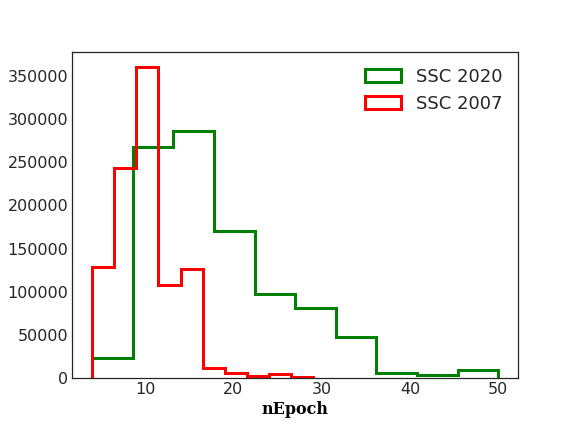
\includegraphics[width=0.4\textwidth, keepaspectratio]{figures/nepoch_compOvsN.png}
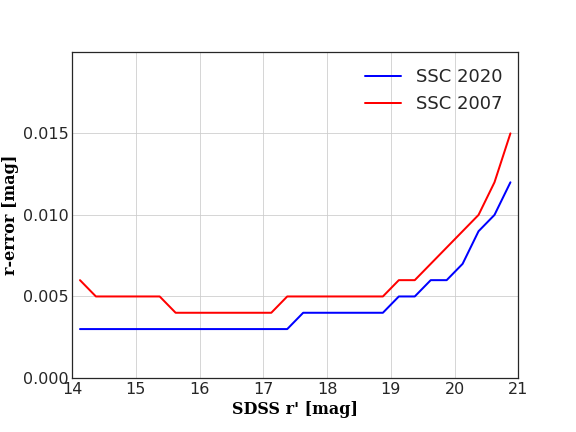
\includegraphics[width=0.4\textwidth, keepaspectratio]{figures/rerr_compOvsN.png}
\caption{{\it Left:} A comparison of the number of observational epochs for matched stars in the 2020 versus 2007 Standard Star Catalog (SSC). {\it Right:} A comparison of the median formal $r$ band photometric uncertainties of matched objects in the 2020 versus 2007 SSC, as a function of their mean $r$ magnitudes.
\label{fig:rerr_nvso}}
\end{figure}


\subsection{The derivation of  photometric zeropoint corrections using Gaia DR2 data\label{sec:GaiaCorr}} 

The variation of photometric zeropoints with position on the sky in the \pOc\ (see their eq.~4) was 
constrained using a combination of stellar colors \citep[the principal axes in color-color diagrams, for details 
see][]{2004AN....325..583I} and a standard star network \citep{2002AJ....123.2121S,2006AN....327..821T}. 
It is likely that residual errors in zeropoint calibration (e.g., a saw-tooth pattern, as a function of Declination,
was reported by \citealt{2013A&A...552A.124B}; see their Fig.~23) can be further minimized using 
uniformly calibrated space-based photometry from Gaia Data Release 2 (DR2). 

\subsubsection{Positional matching of the SDSS and Gaia catalogs}
Naively, one would positionally match the SDSS and Gaia DR2 catalogs using a matching radius of 
about 0.3 arcsec because SDSS positions are accurate to better than 0.1 arcsec per coordinate (rms) 
for sources with $r < 20.5$ mag \citep{2003AJ....125.1559P}.  However, observational epochs are
sufficiently different that stellar proper motions need to be accounted for; indeed, we find a very 
strong correlation between the SDSS-Gaia positional differences and proper motions published in 
the Gaia DR2 catalog (see the left panel in  Figure~\ref{fig:GaiaRApm}). After accounting for proper
motions,  the positions agree at the level of $\sim28$ milliarcsec (robust\footnote{We use robust estimator 
of standard deviation computed as $\sigma_G = 0.741*(q_{75}-q_{25})$, where $q_{25}$ and $q_{75}$ are 
the 25\% and 75\% quantiles, and the normalization factor 0.741 assures that $\sigma_G$ is equal to 
standard deviation for normal (Gaussian) distribution.}
rms, per coordinate). The 
residual differences are dominated by systematic errors in SDSS astrometry because there is
no increase of this rms with magnitude (see the right panel in Figure~\ref{fig:GaiaRApm}), and
because the contribution of Gaia's astrometric measurement uncertainties is negligible. 
The implied SDSS astrometric accuracy of $\sim28$ milliarcsec is substantially better than 
``$<0.1$ arcsec reported by \cite{2003AJ....125.1559P}, but note that here we used 
positions ``averaged'' over typically $\sim20$ SDSS runs (see the left panel in Figure~\ref{fig:rerr_nvso}). 

\begin{figure}[th!]
\centering 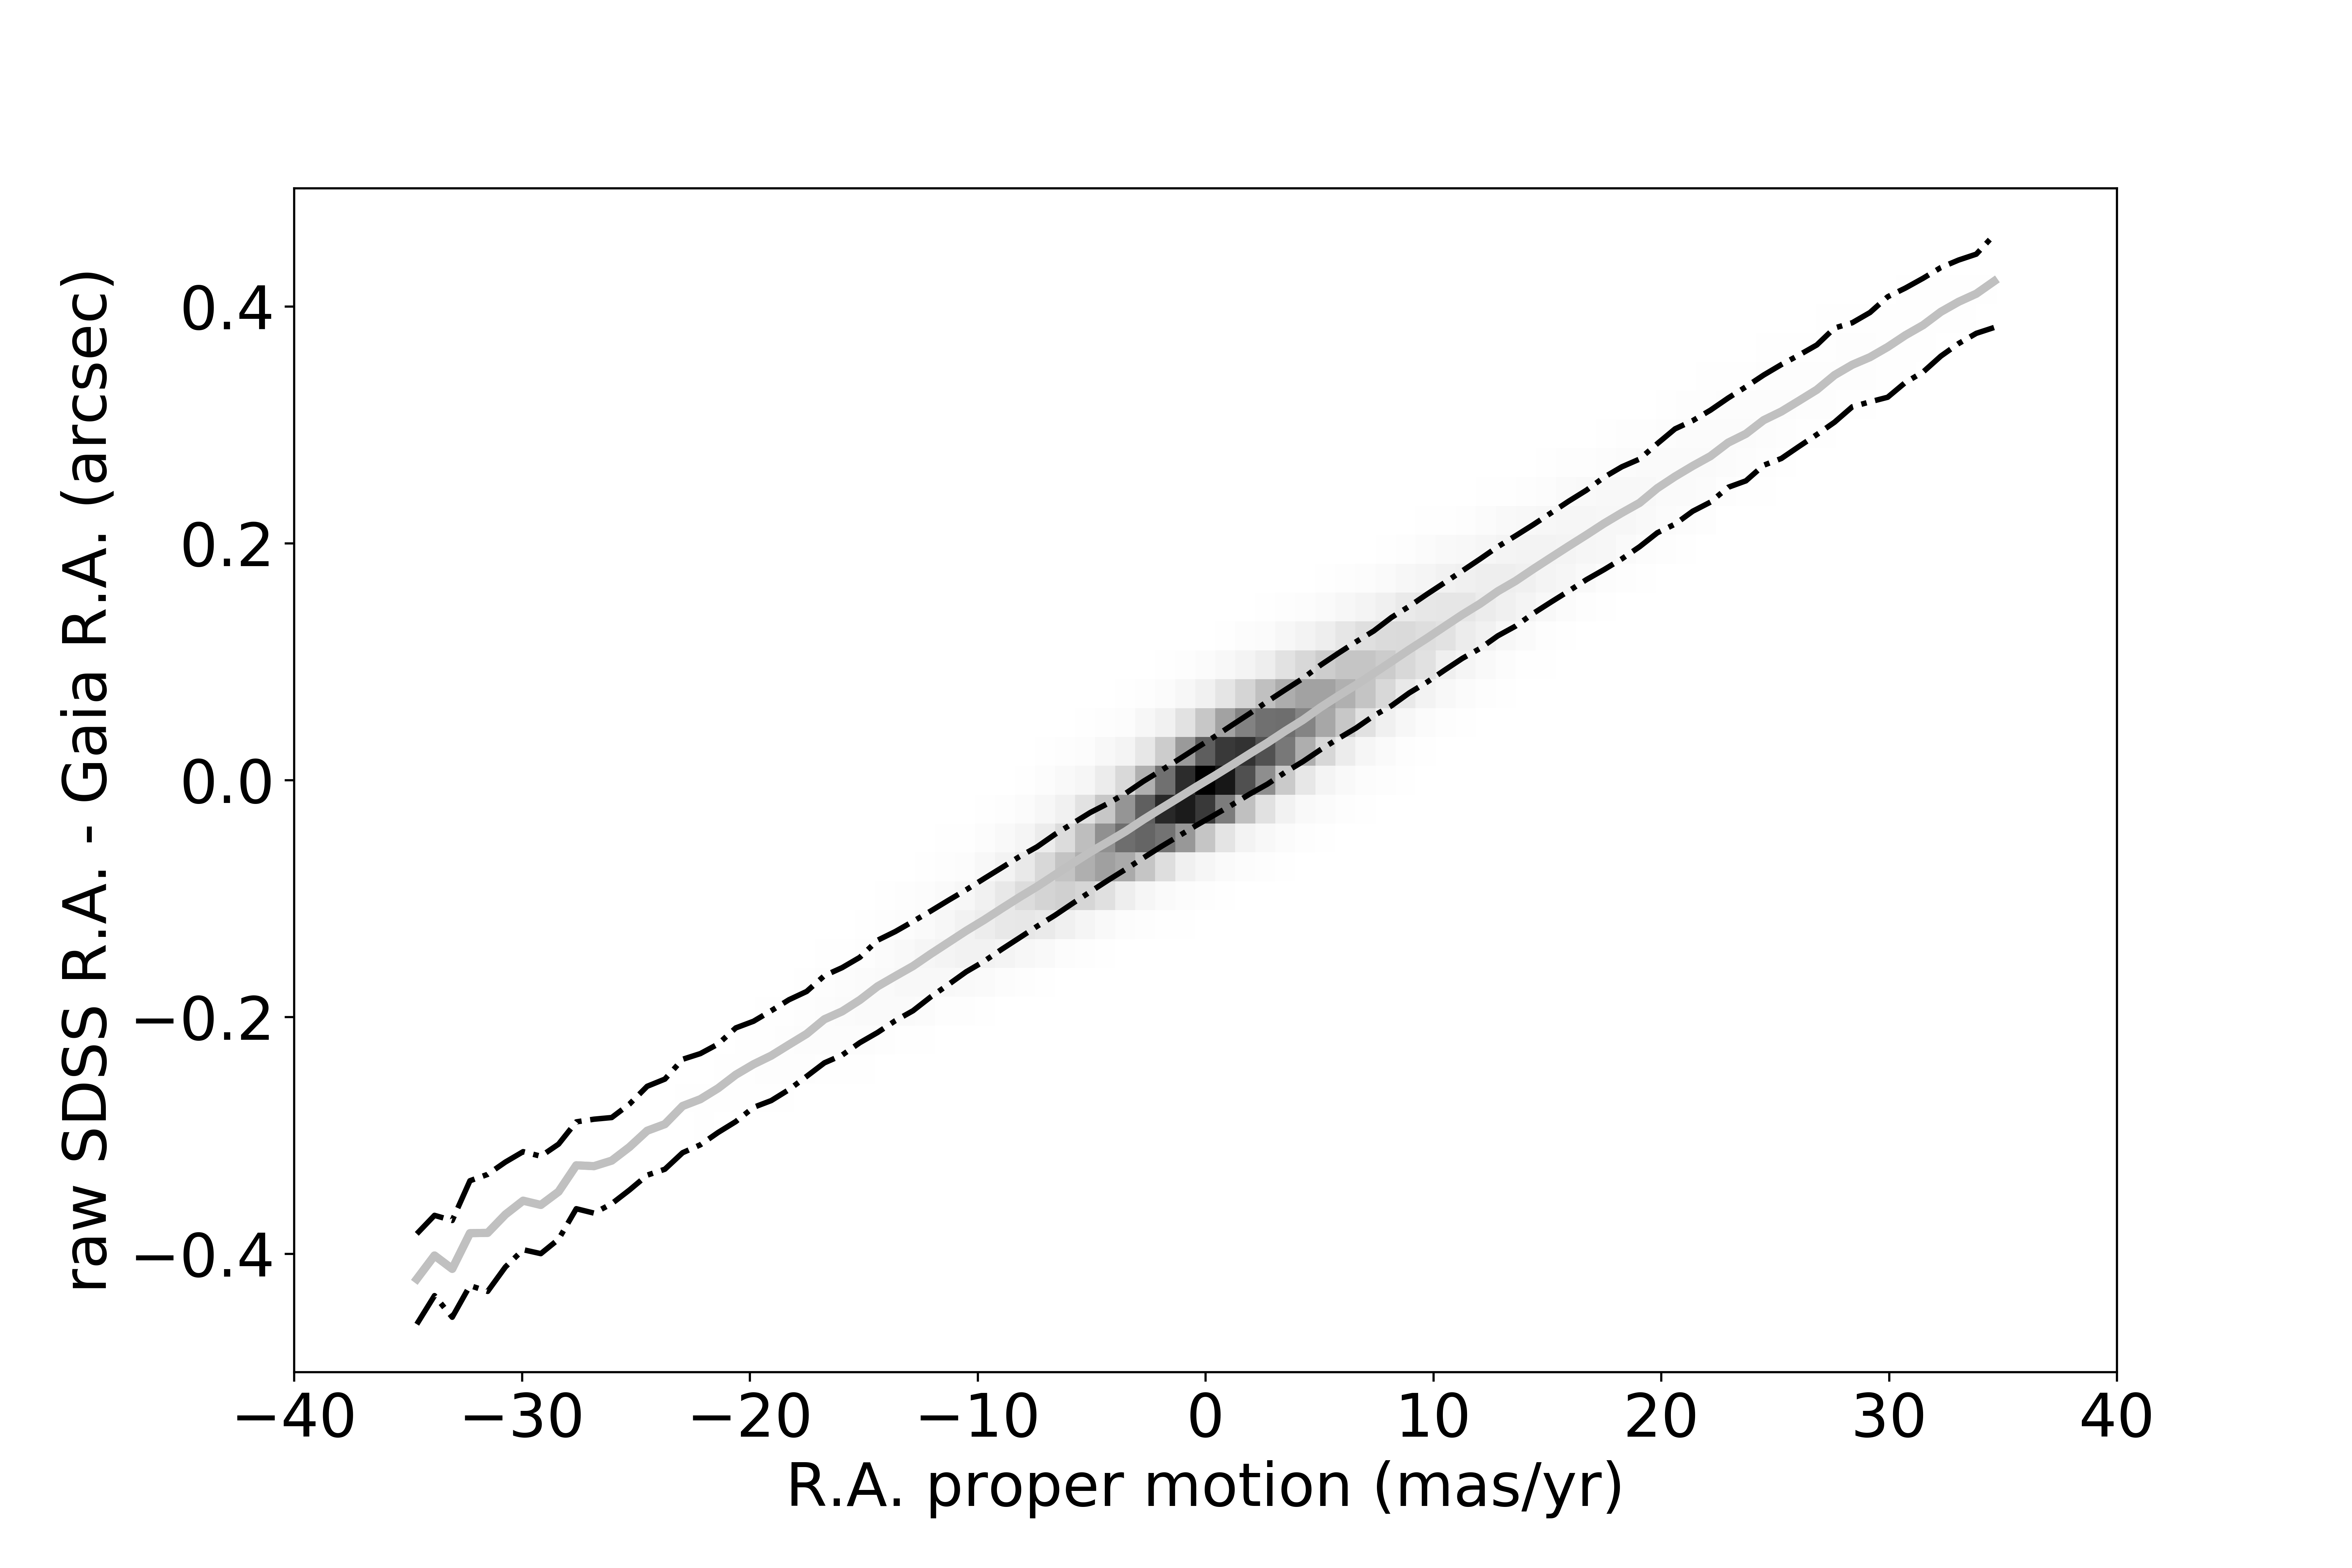
\includegraphics[width=0.4\textwidth, keepaspectratio]{figures/astroVSpm_RA_pm.png}
\centering 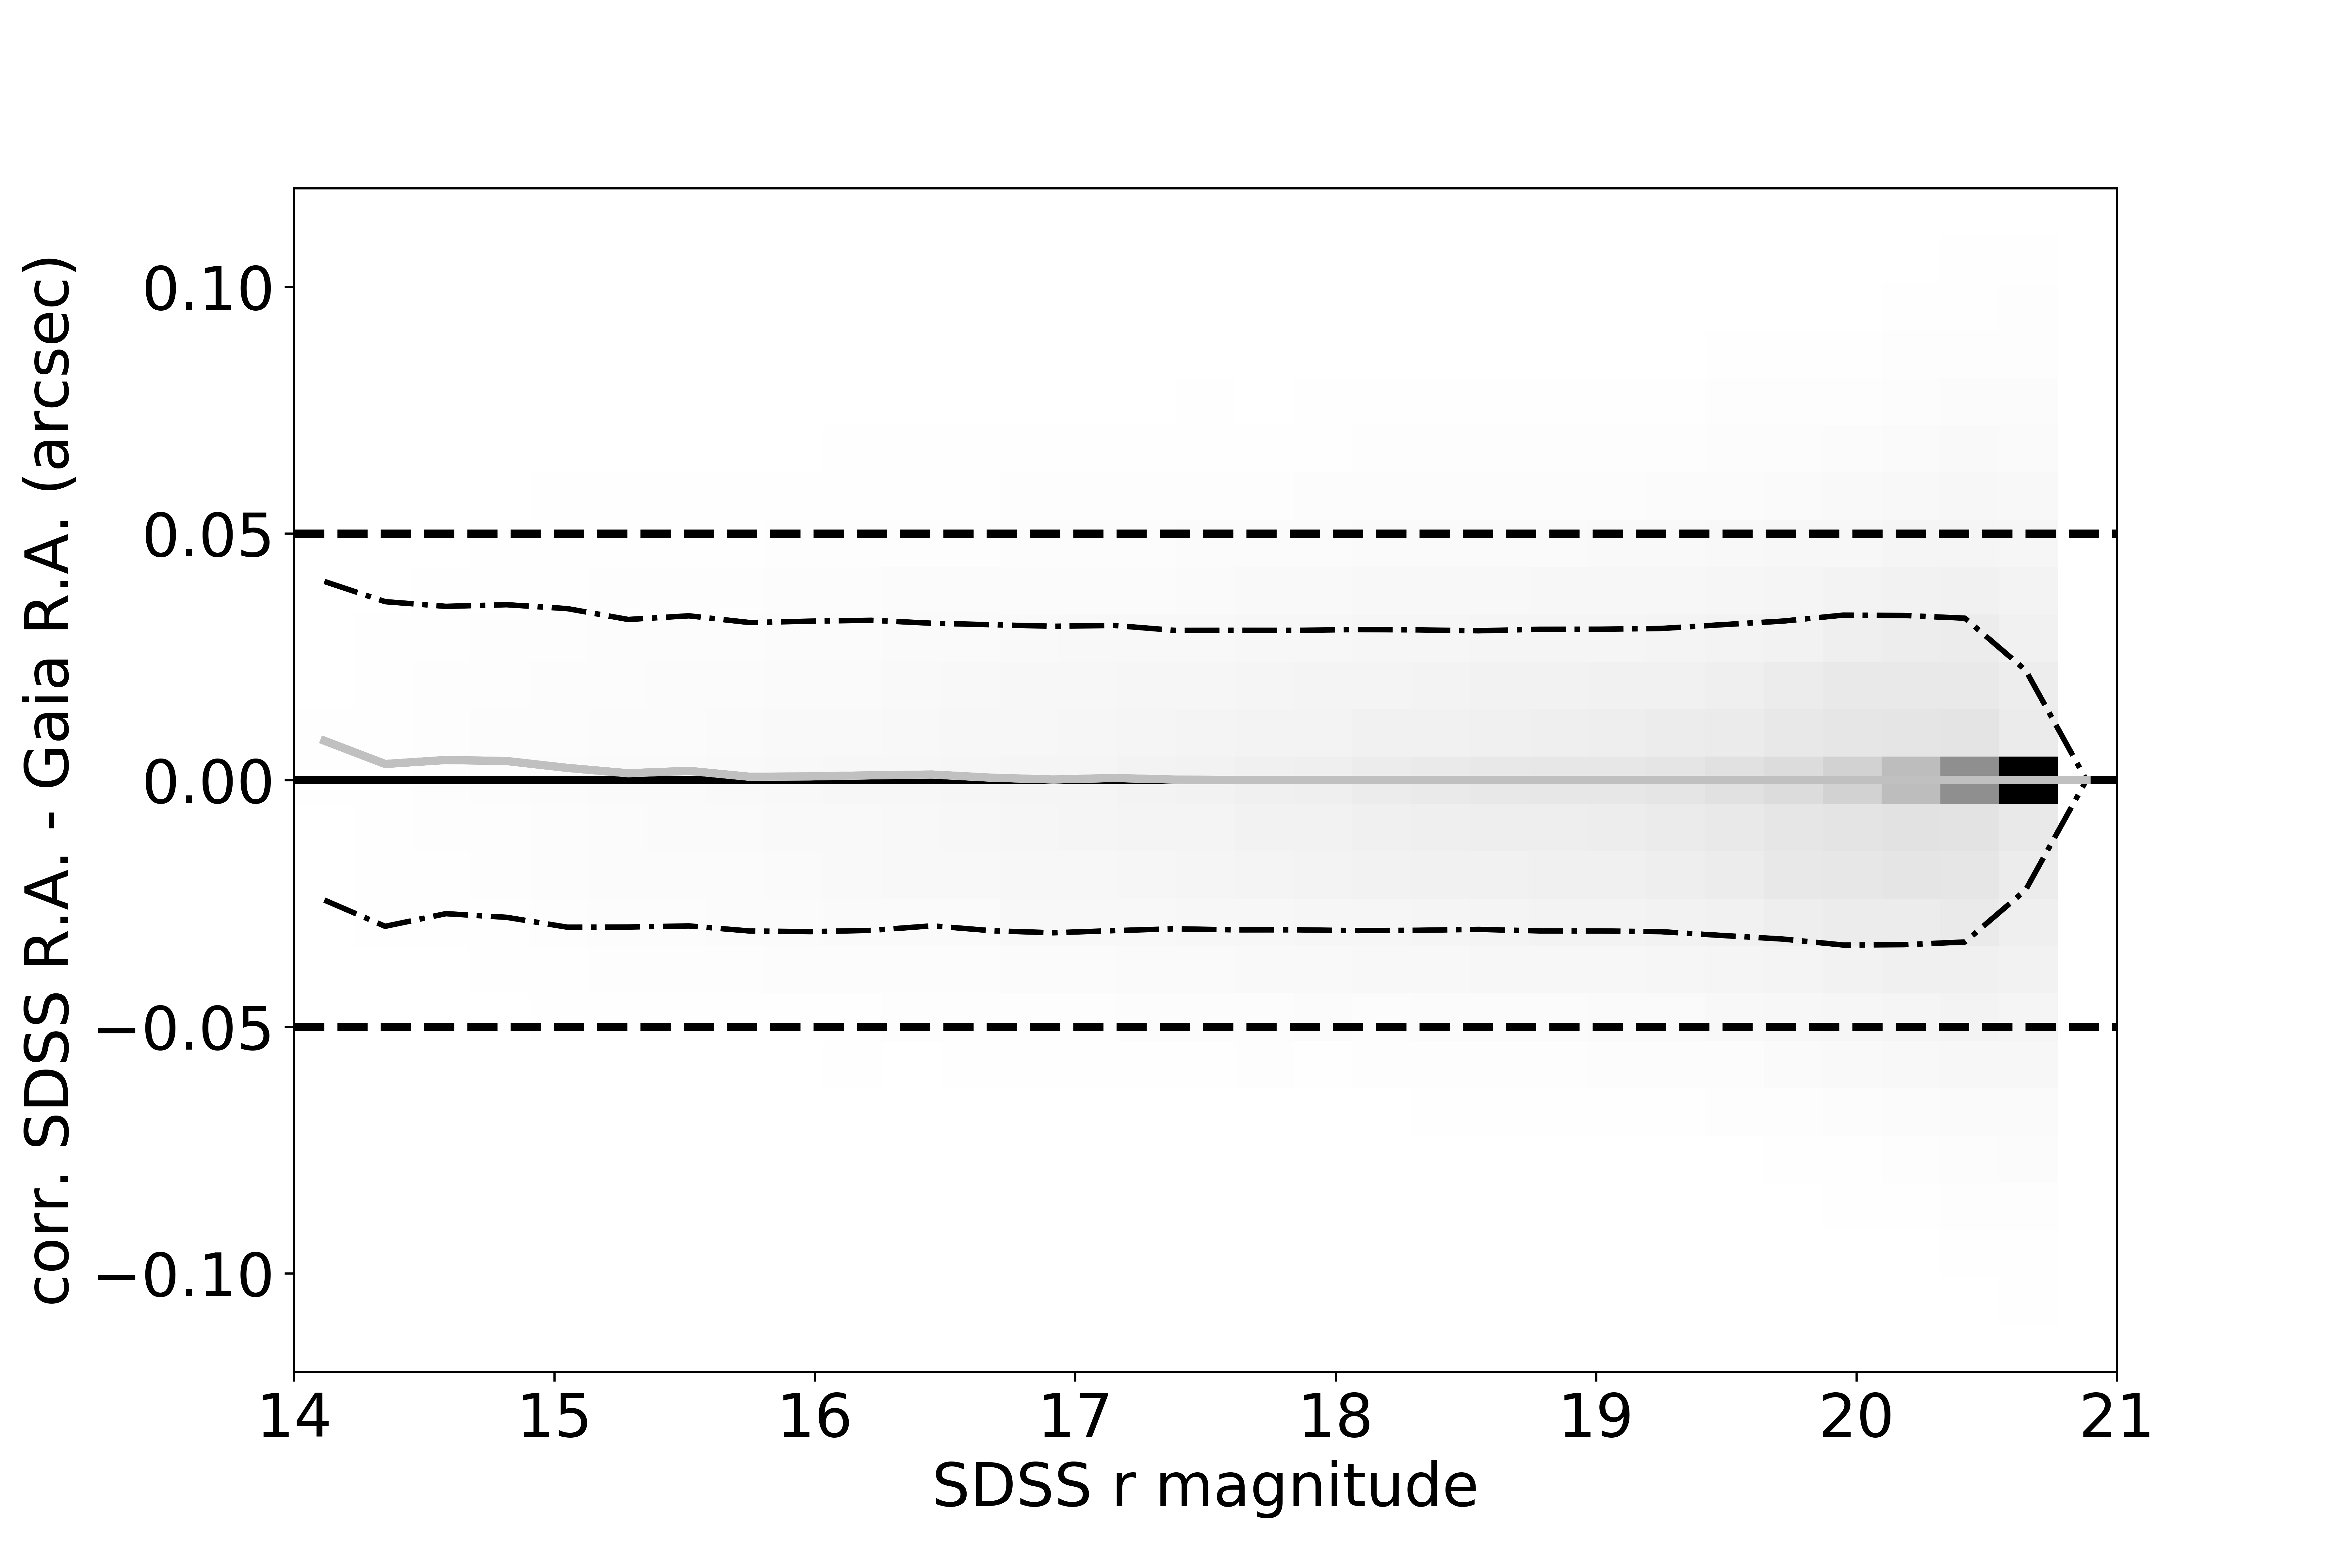
\includegraphics[width=0.4\textwidth, keepaspectratio]{figures/astroVSpm_RA_r.png}

\caption{The left panel shows the R.A. difference between SDSS and Gaia 
vs. R.A. proper motion reported by Gaia DR2. The solid line shows the median difference in bins 
of proper motion and the dashed lines mark the $\pm \sigma_G$ envelope around the medians,
where $\sigma_G$ is the robust standard deviation. The right panel shows the R.A. difference 
after correcting using the best-fit R.A. difference vs. 
proper motion curve, as a function of the SDSS $r$ magnitude. The residual differences are dominated 
by systematic errors in SDSS astrometry at the level of $\sim28$ milliarcsec (note that there is no increase with 
magnitude). Analogous plots for Declination quantities are similar. 
\label{fig:GaiaRApm}}
\end{figure}
  

\subsubsection{Gaia-based photometric zeropoint corrections}

Gaia DR2 reported Gmag magnitudes, which approximately span the SDSS $griz$ bandpasses, 
and BP and RP magnitudes, which approximately correspond to the blue and red halfs of the 
Gmag bandpass. We first used Gmag data to derive ``gray'' zeropoint corrections (applied to
all five SDSS bands), and then use the BP-RP color to derive zeropoint corrections for the 
$ugiz$ bands, relative to the $r$ band. 

The basic idea is simple: use Gaia's Gmag, Gmag$_{GaiaDR2}$, and the SDSS $gri$ magnitudes
to derive synthetic Gmag magnitudes based on SDSS data, Gmag$_{SDSS}$; bin the 
$\Delta$Gmag = (Gmag$_{SDSS}$-Gmag$_{GaiaDR2}$) residuals by R.A. and Dec, and 
use the median residuals per bin as the gray correction for SDSS photometry (as functions
of R.A. and Dec). Similarly, use Gaia's BP-RP color to derive synthetic $u-r$, $g-r$, $r-i$
and $r-z$ colors, and used the median residuals per bin as zeropoint corrections for 
the $ugiz$ bands. 

Given a large number of matched stars ($\sim 400,000$), and a large number of color combinations,
we do not attempt to derive analytic fits for synethtic magnitudes and colors but instead
use 0.05 mag narrow color bins and linear interpolation between the bins. We have verified
that even sixth-order polynomial fits do not provide better results than this simple 
numerical approach. An example of such a transformation is shown in Figure~\ref{fig:GrVSgi}. 


\begin{figure}[th!]
  \centering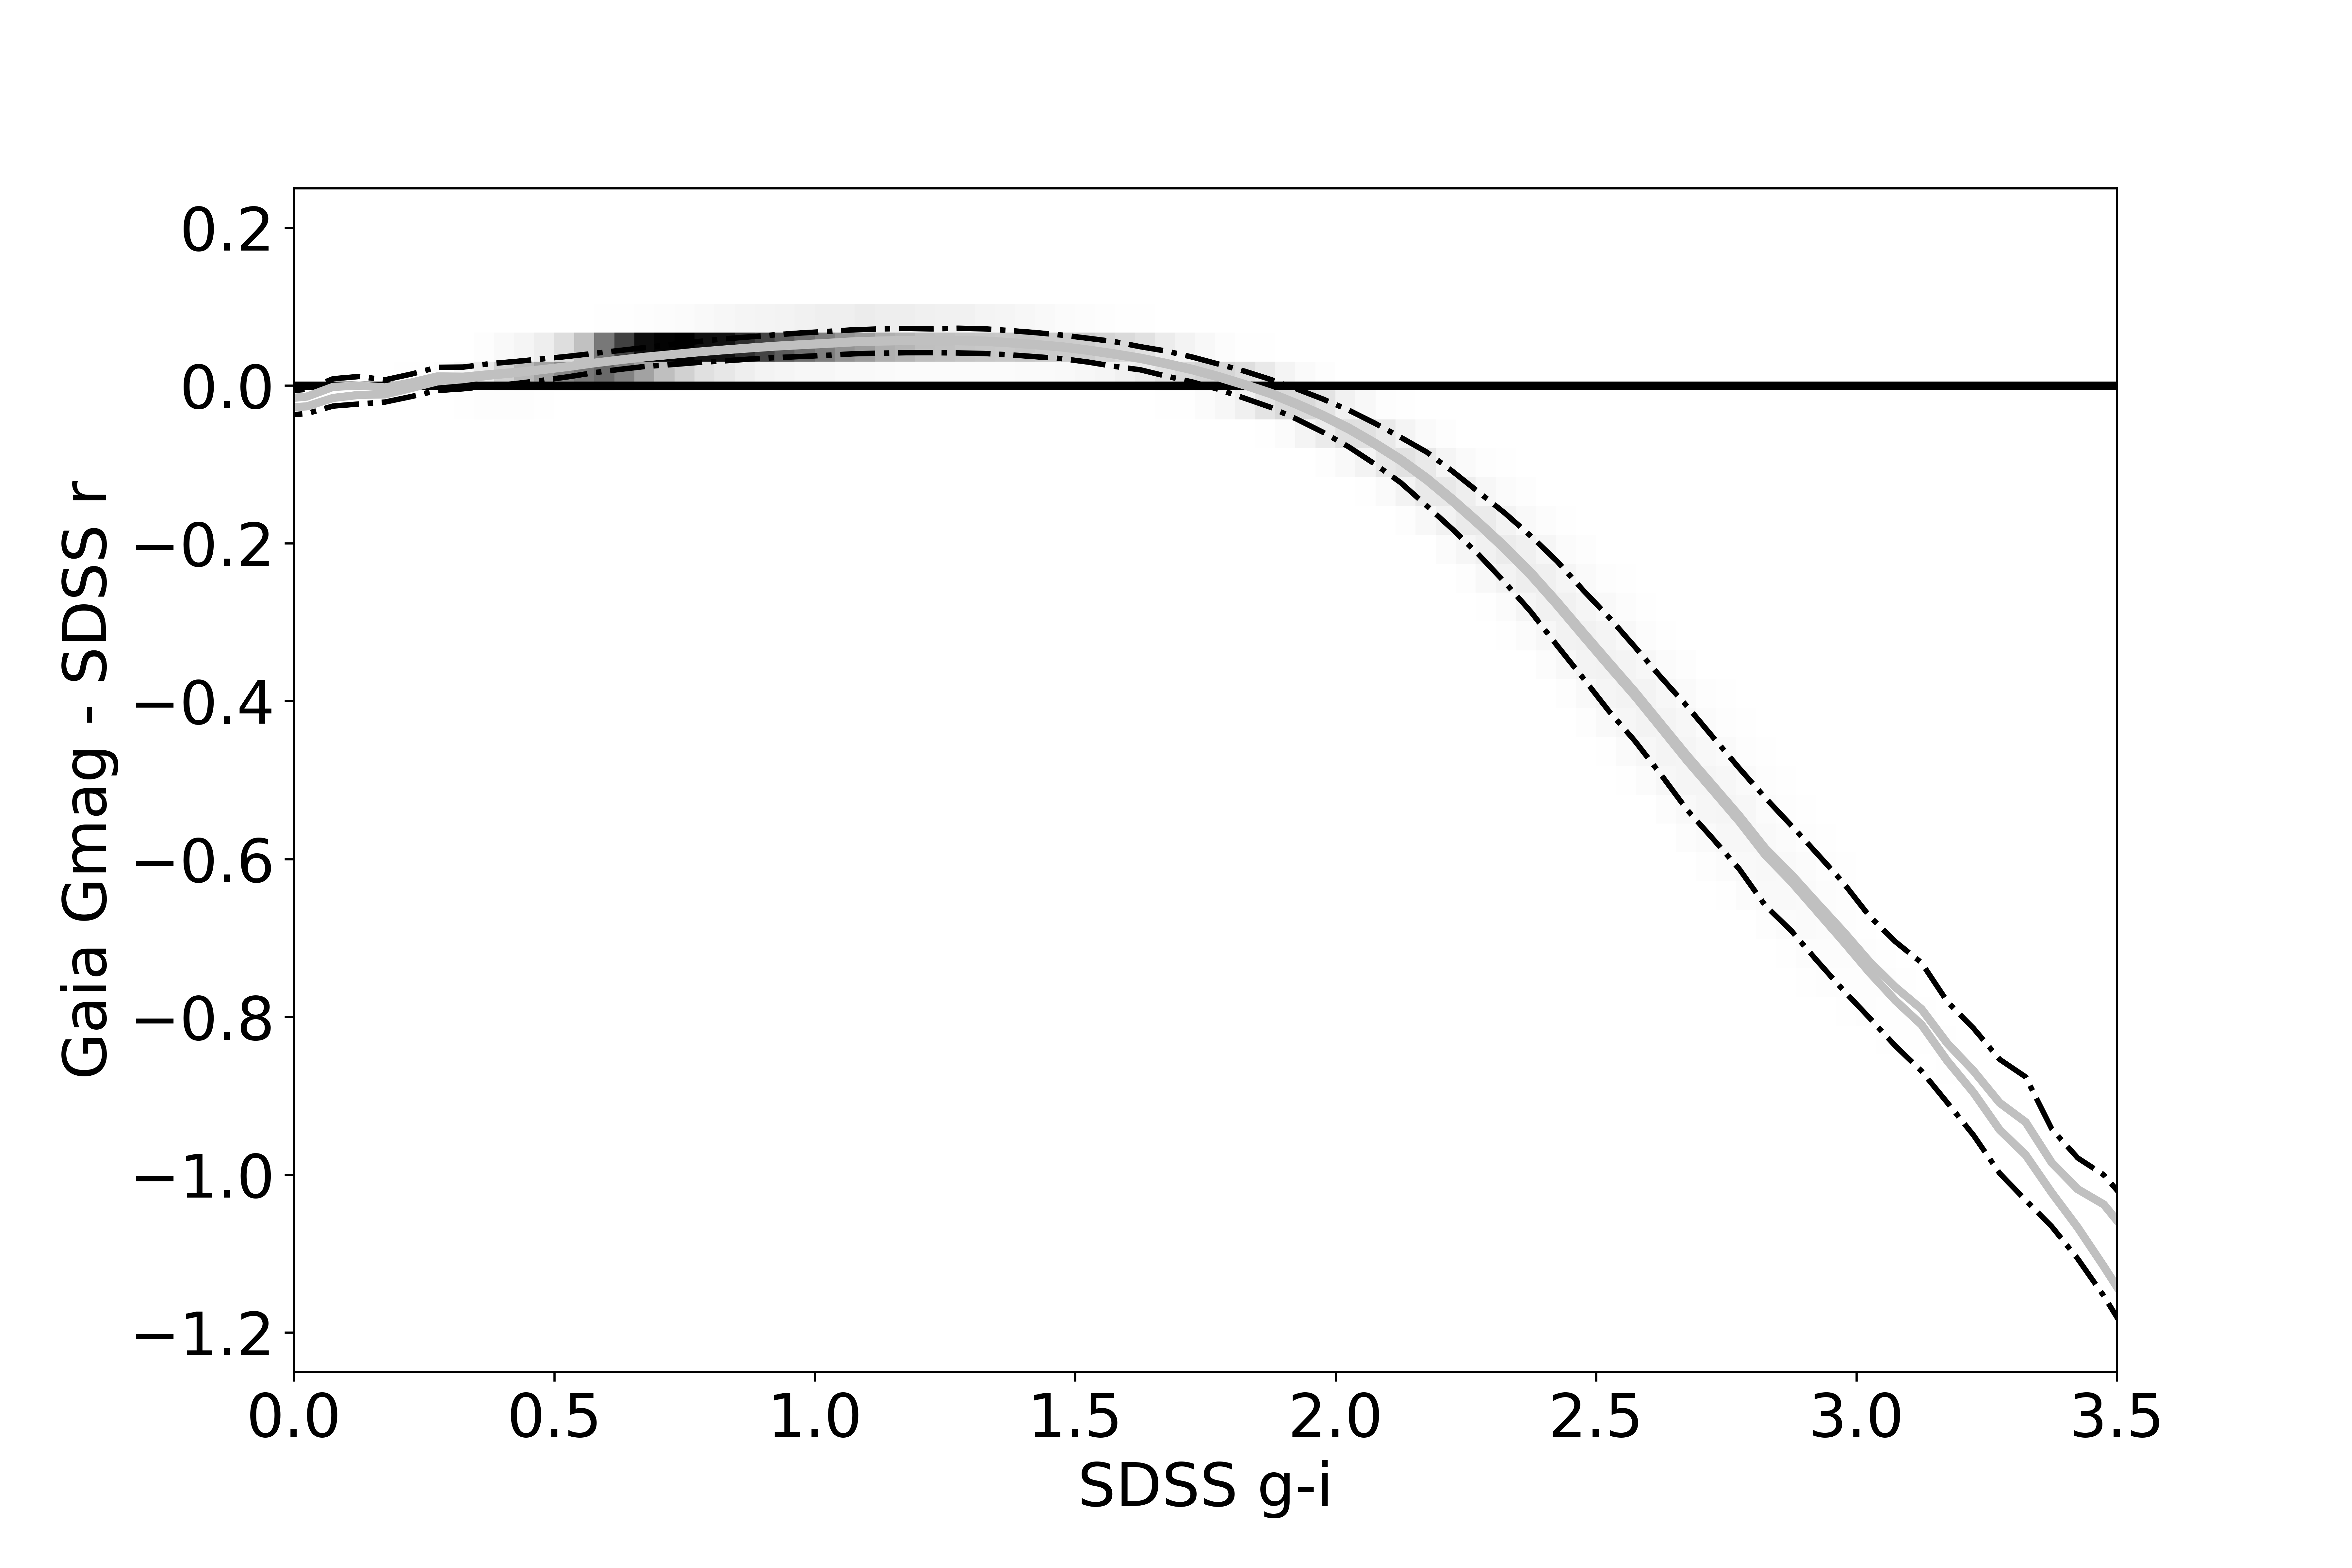
\includegraphics[width=8cm]{figures/GrVSgi.png} 
\caption{The variation of the difference between Gaia's Gmag magnitude from Data Release 2
and SDSS $r$ magnitude with the SDSS $g-i$ color.
The  color map illustrates the distribution of $\sim 393,000$ matched stars with 
$16<$Gmag$<19.5$. The two (barely distinguishable) solid lines represent the median 
values $\pm$ uncertainty of the median for 0.05 mag wide $g-i$ bins. The short-dashed 
lines show the median values $\pm$ the robust standard deviation for 
each bin. The horizontal solid line at zero is added to guide the eye. The mean of 
the two solid lines is used to derive the gray zeropoint correction, as a function of R.A.
and Declination.}
\label{fig:GrVSgi}
\end{figure}


The variation of Gmag residuals with Gmag (see Figure~\ref{fig:gaiaJump}) shows two 
interesting features. First, there is a sharp
``jump'' by about 3 millimag at Gmag$\sim$16.  This jump was a known (and 
larger problem) in Gaia Data Release 1, but appears not entirely fixed in DR2. The 
second ``feature'' is a large ($\sim0.01-0.02$ mag) discrepancy at the faint end:
about $\sim$10 millimag at Gmag=19.5 and $\sim$20 millimag at Gmag=20.5. 
A comparison of the SDSS catalog with Pan-STARRS and DES catalogs (see 
Section~\ref{sec:DESPS1} and Figure~\ref{fig:drVSr}) strongly suggests that the
origin of this discrepancy is a bias in Gaia's Gmag photometry at the faint end, rather 
than a problem with SDSS catalog (offsets between the SDSS and DES
photometry are $<1-2$ millimag at Gmag$\sim$20.5). 
 

\begin{figure}[th!]
    \centering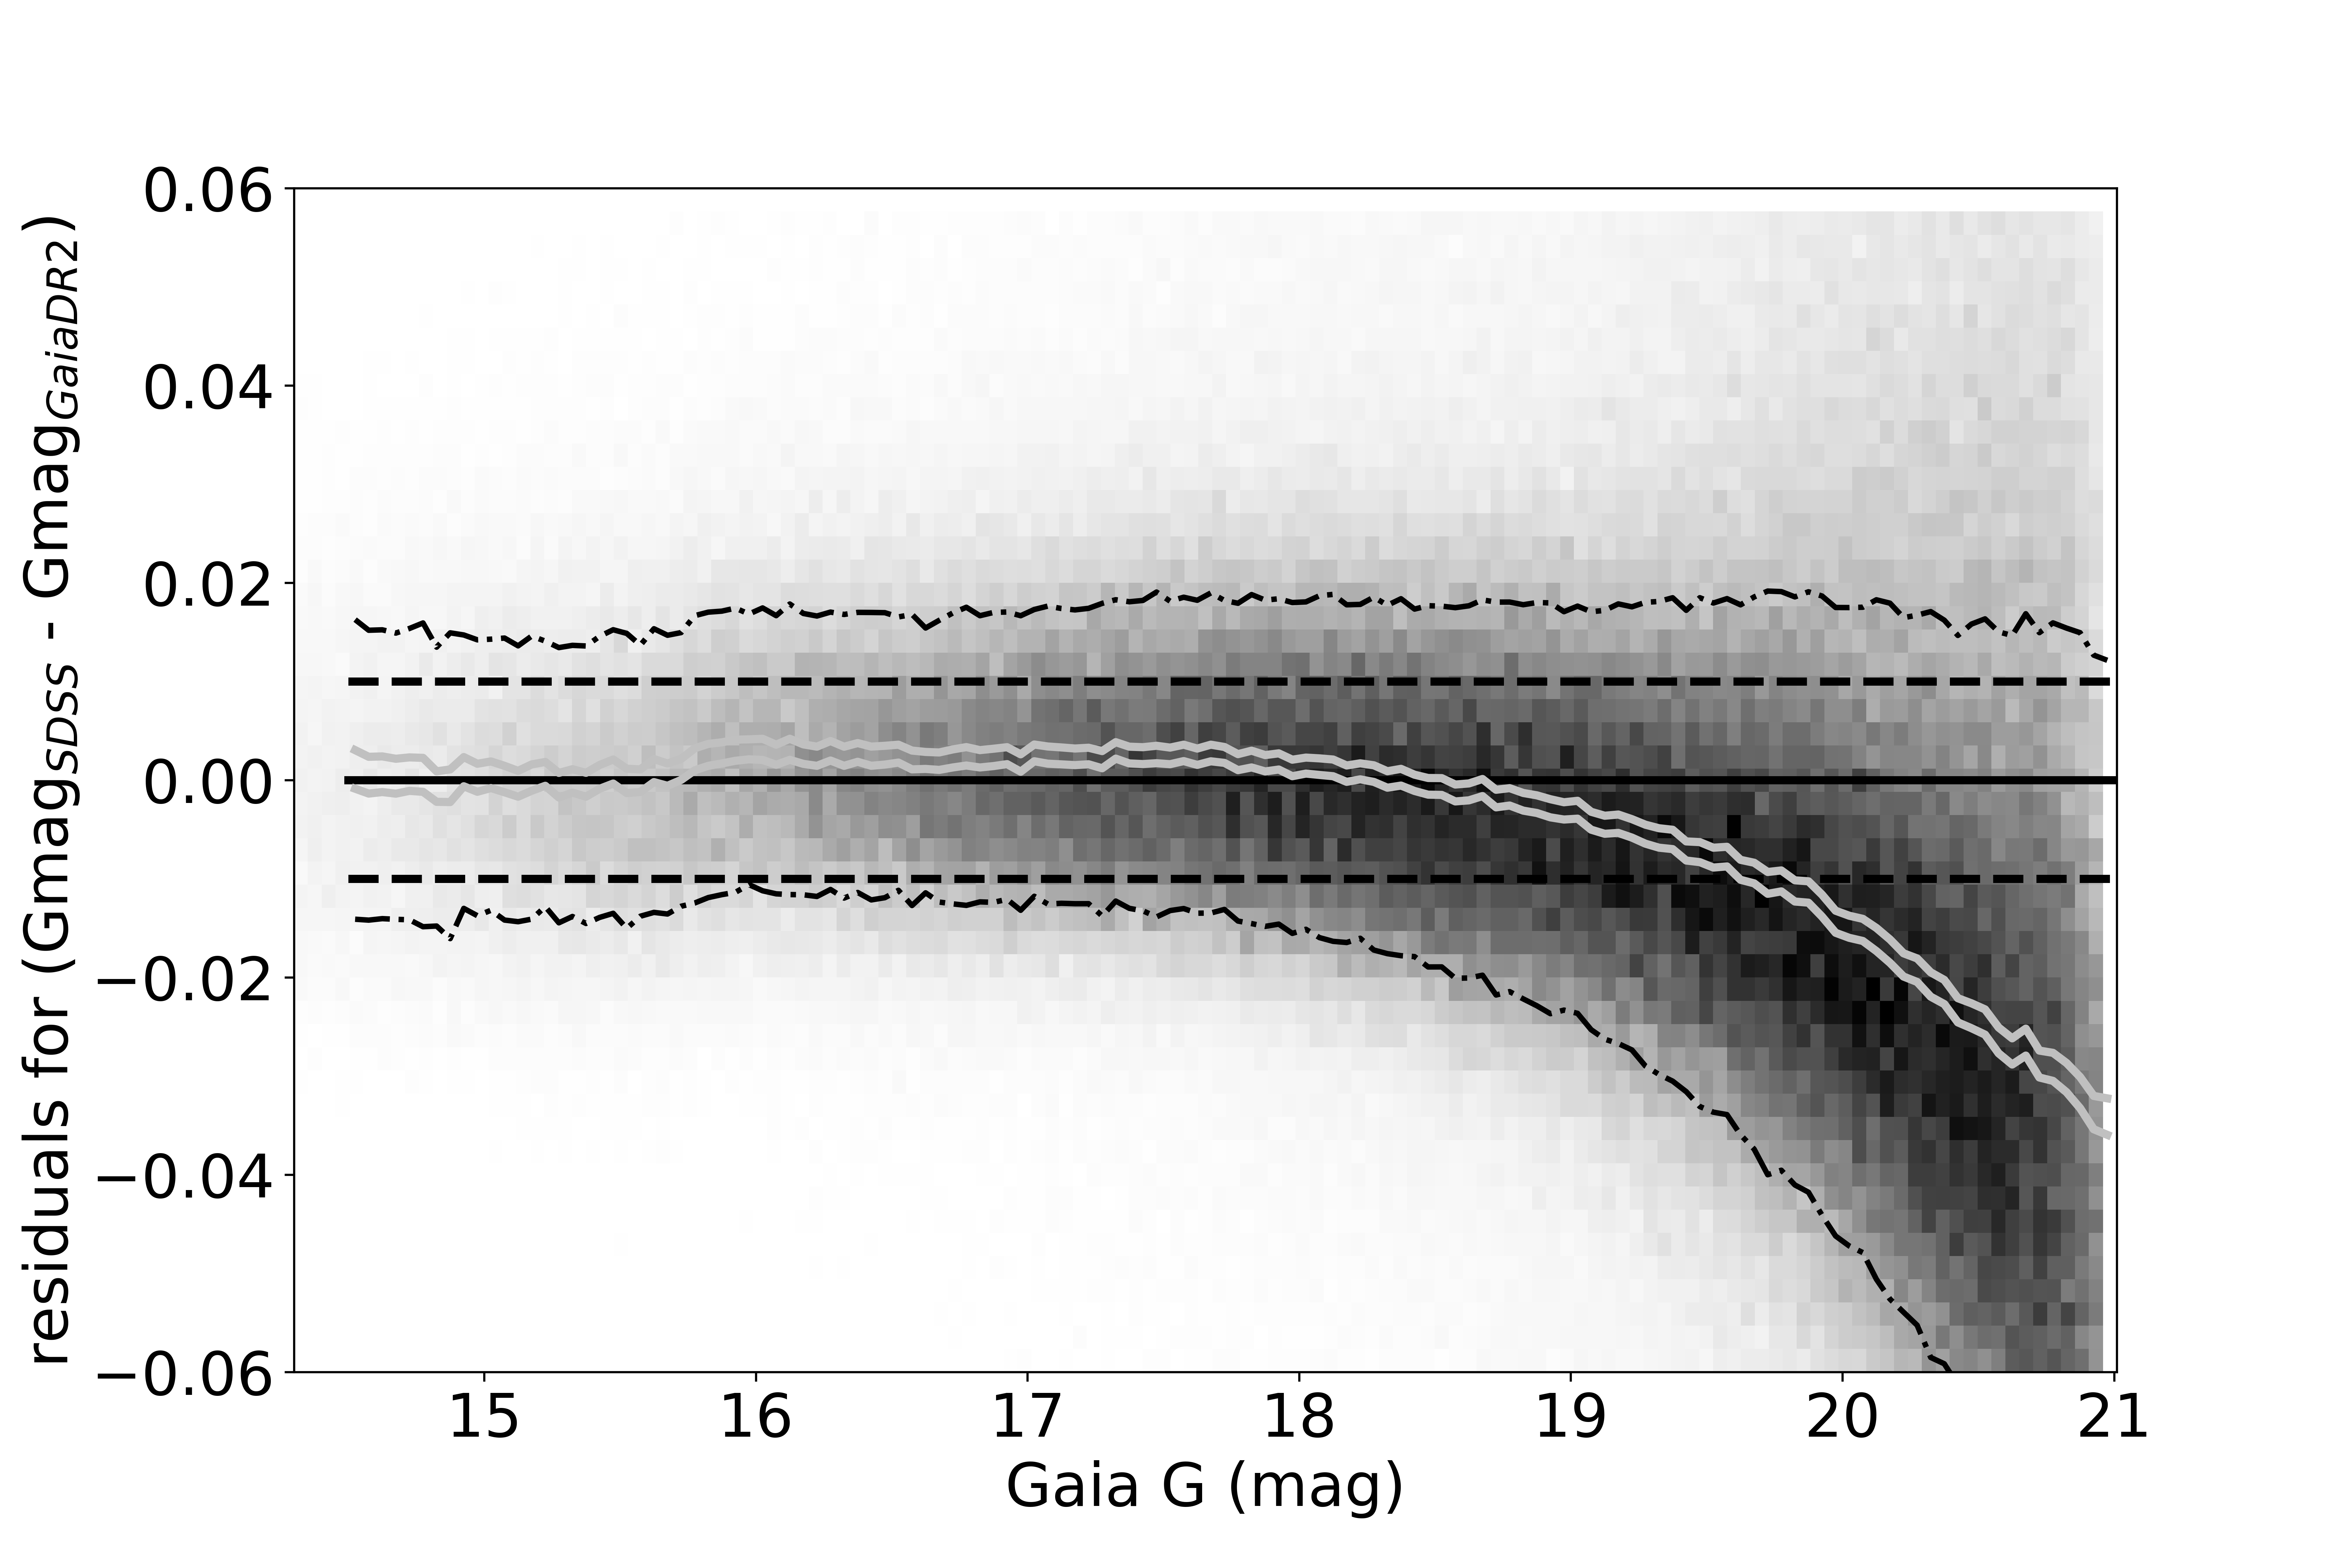
\includegraphics[width=9cm]{figures/GmagCorrectionTest_Gmag_Hess.png} 
\caption{The variation of the residuals between Gaia's Gmag from Data Release 2
and synthetic Gmag values generated using SDSS $gri$ photometry. The two solid 
lines represent the median values $\pm$ uncertainty of the median for each
0.05 mag wide Gmag bin. The short-dashed lines show the median values $\pm$ 
the robust standard deviation for each bin. The horizontal solid and long-dashed 
lines at zero and $\pm$0.01 mag, respectively, are added to guide the eye.
Note the jump by about 3 millimag at Gmag$\sim$16 -- this jump was a known and 
larger problem in Gaia Data Release 1, and apparently not entirely fixed in DR2. 
Note also large ($\sim0.01-0.02$ mag) discrepancy at the faint end -- a comparison 
of the SDSS catalog with Pan-STARRS and DES catalogs (see Figure~\ref{fig:drVSr}) 
suggests that its origin is a bias in Gaia's photometry at the faint end, rather than 
a problem with SDSS photometry.}
\label{fig:gaiaJump}
\end{figure}


Given these two features, we limit the calibration sample to the $16<$Gmag$<19.5$
magnitude range. We further restrict calibration stars to the $0.4 < g-i < 3.0$ color 
range (approximately A0 to M5 spectral range), yielding a sample of $\sim372,000$ stars. 
The behavior of median Gmag residuals per R.A. and Declination bin is shown in 
Figures~\ref{fig:graycorrRA} and \ref{fig:graycorrDec}. 


\begin{figure}[th!]
  \centering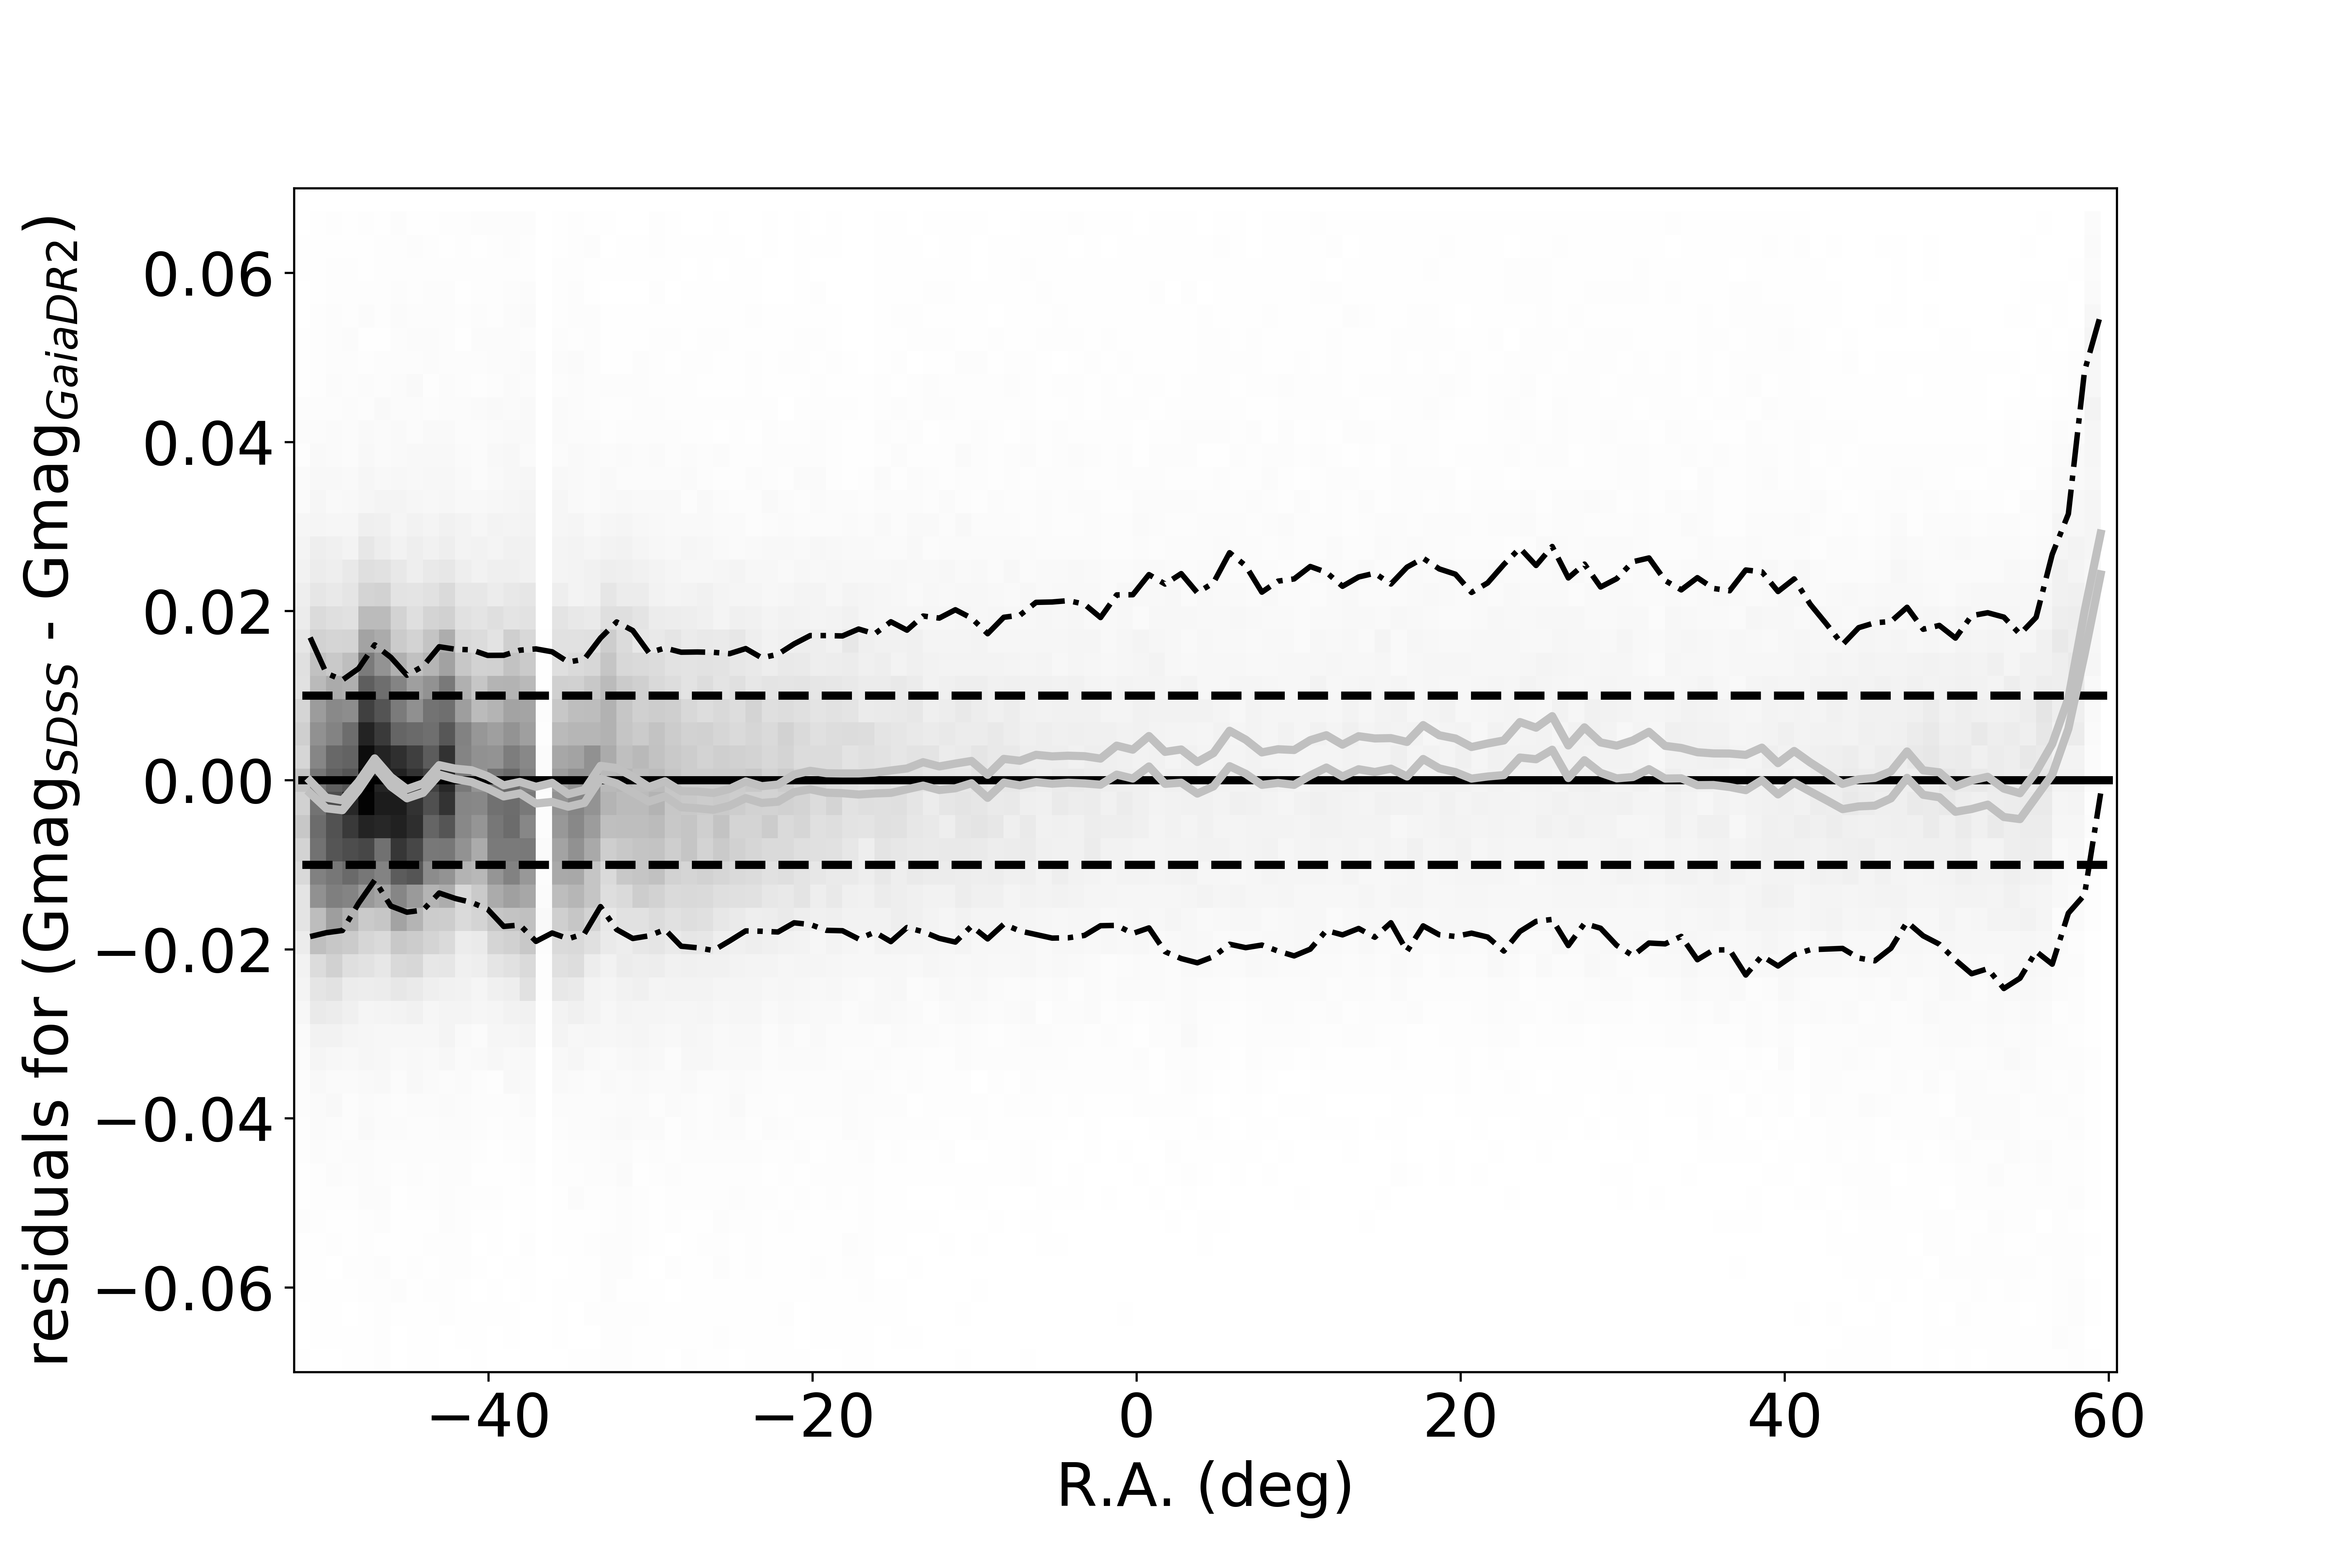
\includegraphics[width=8cm]{figures/GmagCorrection_RA_Hess.png} 
\caption{The R.A. variation of the residuals between Gaia's Gmag from DR2
and synthetic Gmag values generated using SDSS $gri$ photometry. The 
color map illustrates the distribution of $\sim 372,000$ matched stars with 
$16<$Gmag$<19.5$ and $0.4 < g-i < 3.0$. The two solid lines represent the 
median values $\pm$ uncertainty of the median for 1 degree wide R.A. bins. 
The short-dashed lines show the median values $\pm$ the robust standard 
deviation for each bin. The horizontal solid and long-dashed lines at zero and 
$\pm$0.01 mag, respectively, are added to guide the eye. The mean of the two 
solid lines is the gray correction, as a function of R.A., applied to the SDSS 
$ugriz$ magnitudes. The standard deviation for the applied correction is 3.5 millimag.}
\label{fig:graycorrRA}
\end{figure}

\begin{figure}[th!]
    \centering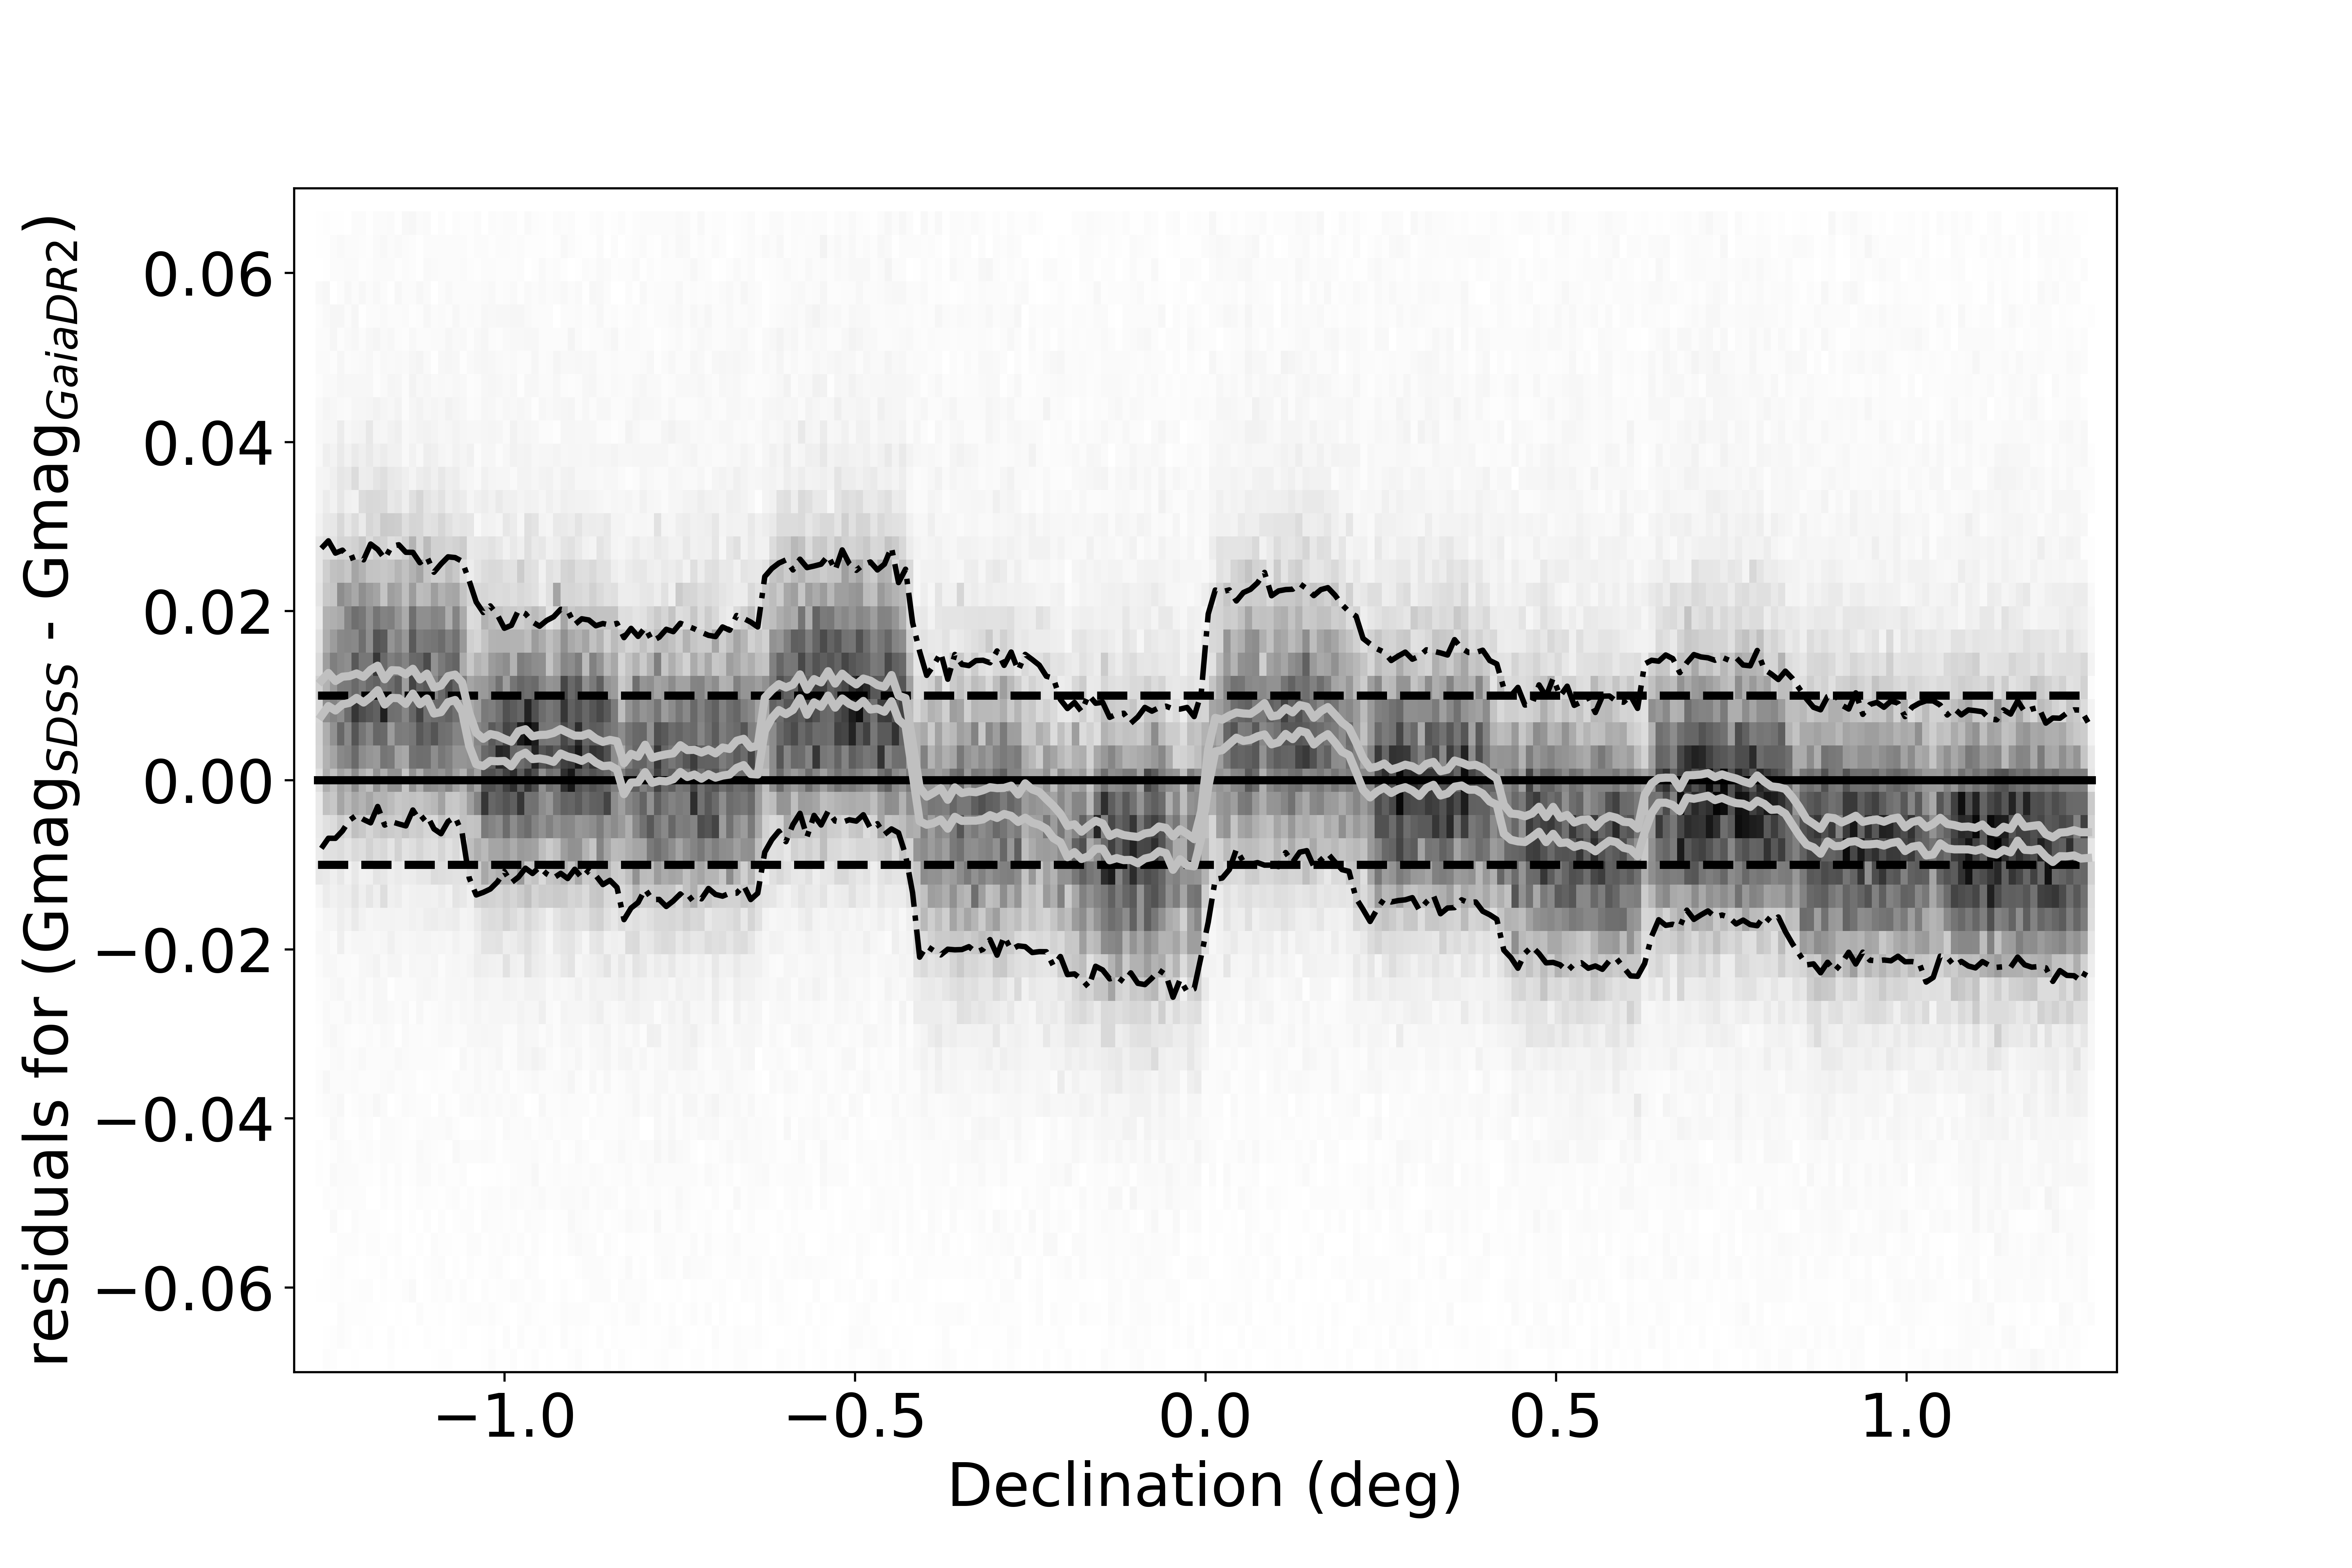
\includegraphics[width=9cm]{figures/GmagCorrection_Dec_Hess.png} 
\caption{Analogous to Figure~\ref{fig:graycorrRA}, except that here results are shown for
0.01 degree wide Declination bins. The 12 cleary visible regions correspond to
two SDSS scans (in R.A. direction) and six CCD columns in the SDSS camera. 
The standard deviation for the applied correction is 6.2 millimag, with a maximum
absolute value of $\sim0.01$ mag.}
\label{fig:graycorrDec}
\end{figure}


Except for a few degrees long region at the edge of Stripe 82 (R.A.$>$55 deg), the
SDSS photometric zeropoints are remarkably stable with respect to R.A.; the scatter
is only 3.5 millimag. On the other hand, there are clear deviations in Declination 
direction, which clearly map to the 12 scanning strips that fill Stripe 82. We note
that discrepancies never exceed 0.01 mag (with a scatter of 6.2 millimag), which was 
the claimed accuracy of the \pOc. Thanks to a large number of stars in the sample,
and well calibrated Gaia's photometric zeropoints across the sky, we can now 
constrain SDSS zeropoints with a precision of about 1 millimag per 0.01 degree
wide Declination bin. 

The residuals shown in Figures~\ref{fig:graycorrRA} and \ref{fig:graycorrDec} are
applied as ``gray'' zeropoint corrections to $ugriz$ magnitudes, as functions of 
R.A. and Declination, to all 991,472 stars in the catalog. This catalog version was
labeled v3.1, and it is publicly available\footnote{See http://faculty.washington.edu/ivezic/sdss/catalogs/stripe82.html}. 

In the next re-calibration step, we derive synthetic $u-r$, $g-r$, $r-i$ and $r-z$ colors
from Gaia's BP-RP color, using the same binning procedure as we used above for 
Gmag$-r$ vs. $g-i$ variation (see Figure~\ref{fig:GrVSgi}). An example of color residuals 
is shown in Figure~\ref{fig:riresid}.  The median residuals per R.A. and Declination bins 
are then used as zeropoint corrections for the $ugiz$ bands. We required that the median
offsets for all stars are vanishing and thus photometry in the new catalog is on the 
same AB scale as the old catalog (for related discussion, see Section~\ref{sec:AB}). 
The robust standard deviation for all zeropoint corrections is listed in Table~\ref{tab:GaiaRMS}. 

\begin{deluxetable}{l|c|c}[ht!]
\tablecaption{The robust standard deviation for binned SDSS-based vs. Gaia-based color residuals$^a$. \label{tab:GaiaRMS}}
\tablehead{
\colhead{Color } & \colhead{rms for R.A.} & \colhead{rms for Dec}
}
\startdata
 gray (Gmag) &    3.5         &    6.2   \\
    $u-r$        &   0.0$^b$  &   20.4   \\     
    $g-r$        &   4.0         &    4.2    \\
    $r-i$         &   4.1         &    3.2    \\ 
    $r-z$        &   7.4         &    2.9    \\ 
\enddata
\tablenotetext{a}{The standard deviation for applied Gaia-based zeropoint corrections. The robust standard deviation 
is estimated using interquartile range. The units are millimag.} 
\tablenotetext{b}{For the $u$ band, we could not confirm the R.A. behavior of Gaia-based zeropoint correction 
with the CFIS data and didn't apply it. The large $u$ band correction as a function of Declination was validated 
with the CFIS data (see Section~\ref{sec:CFIStest}).} 
\end{deluxetable}
 

\begin{figure}[th!]
    \centering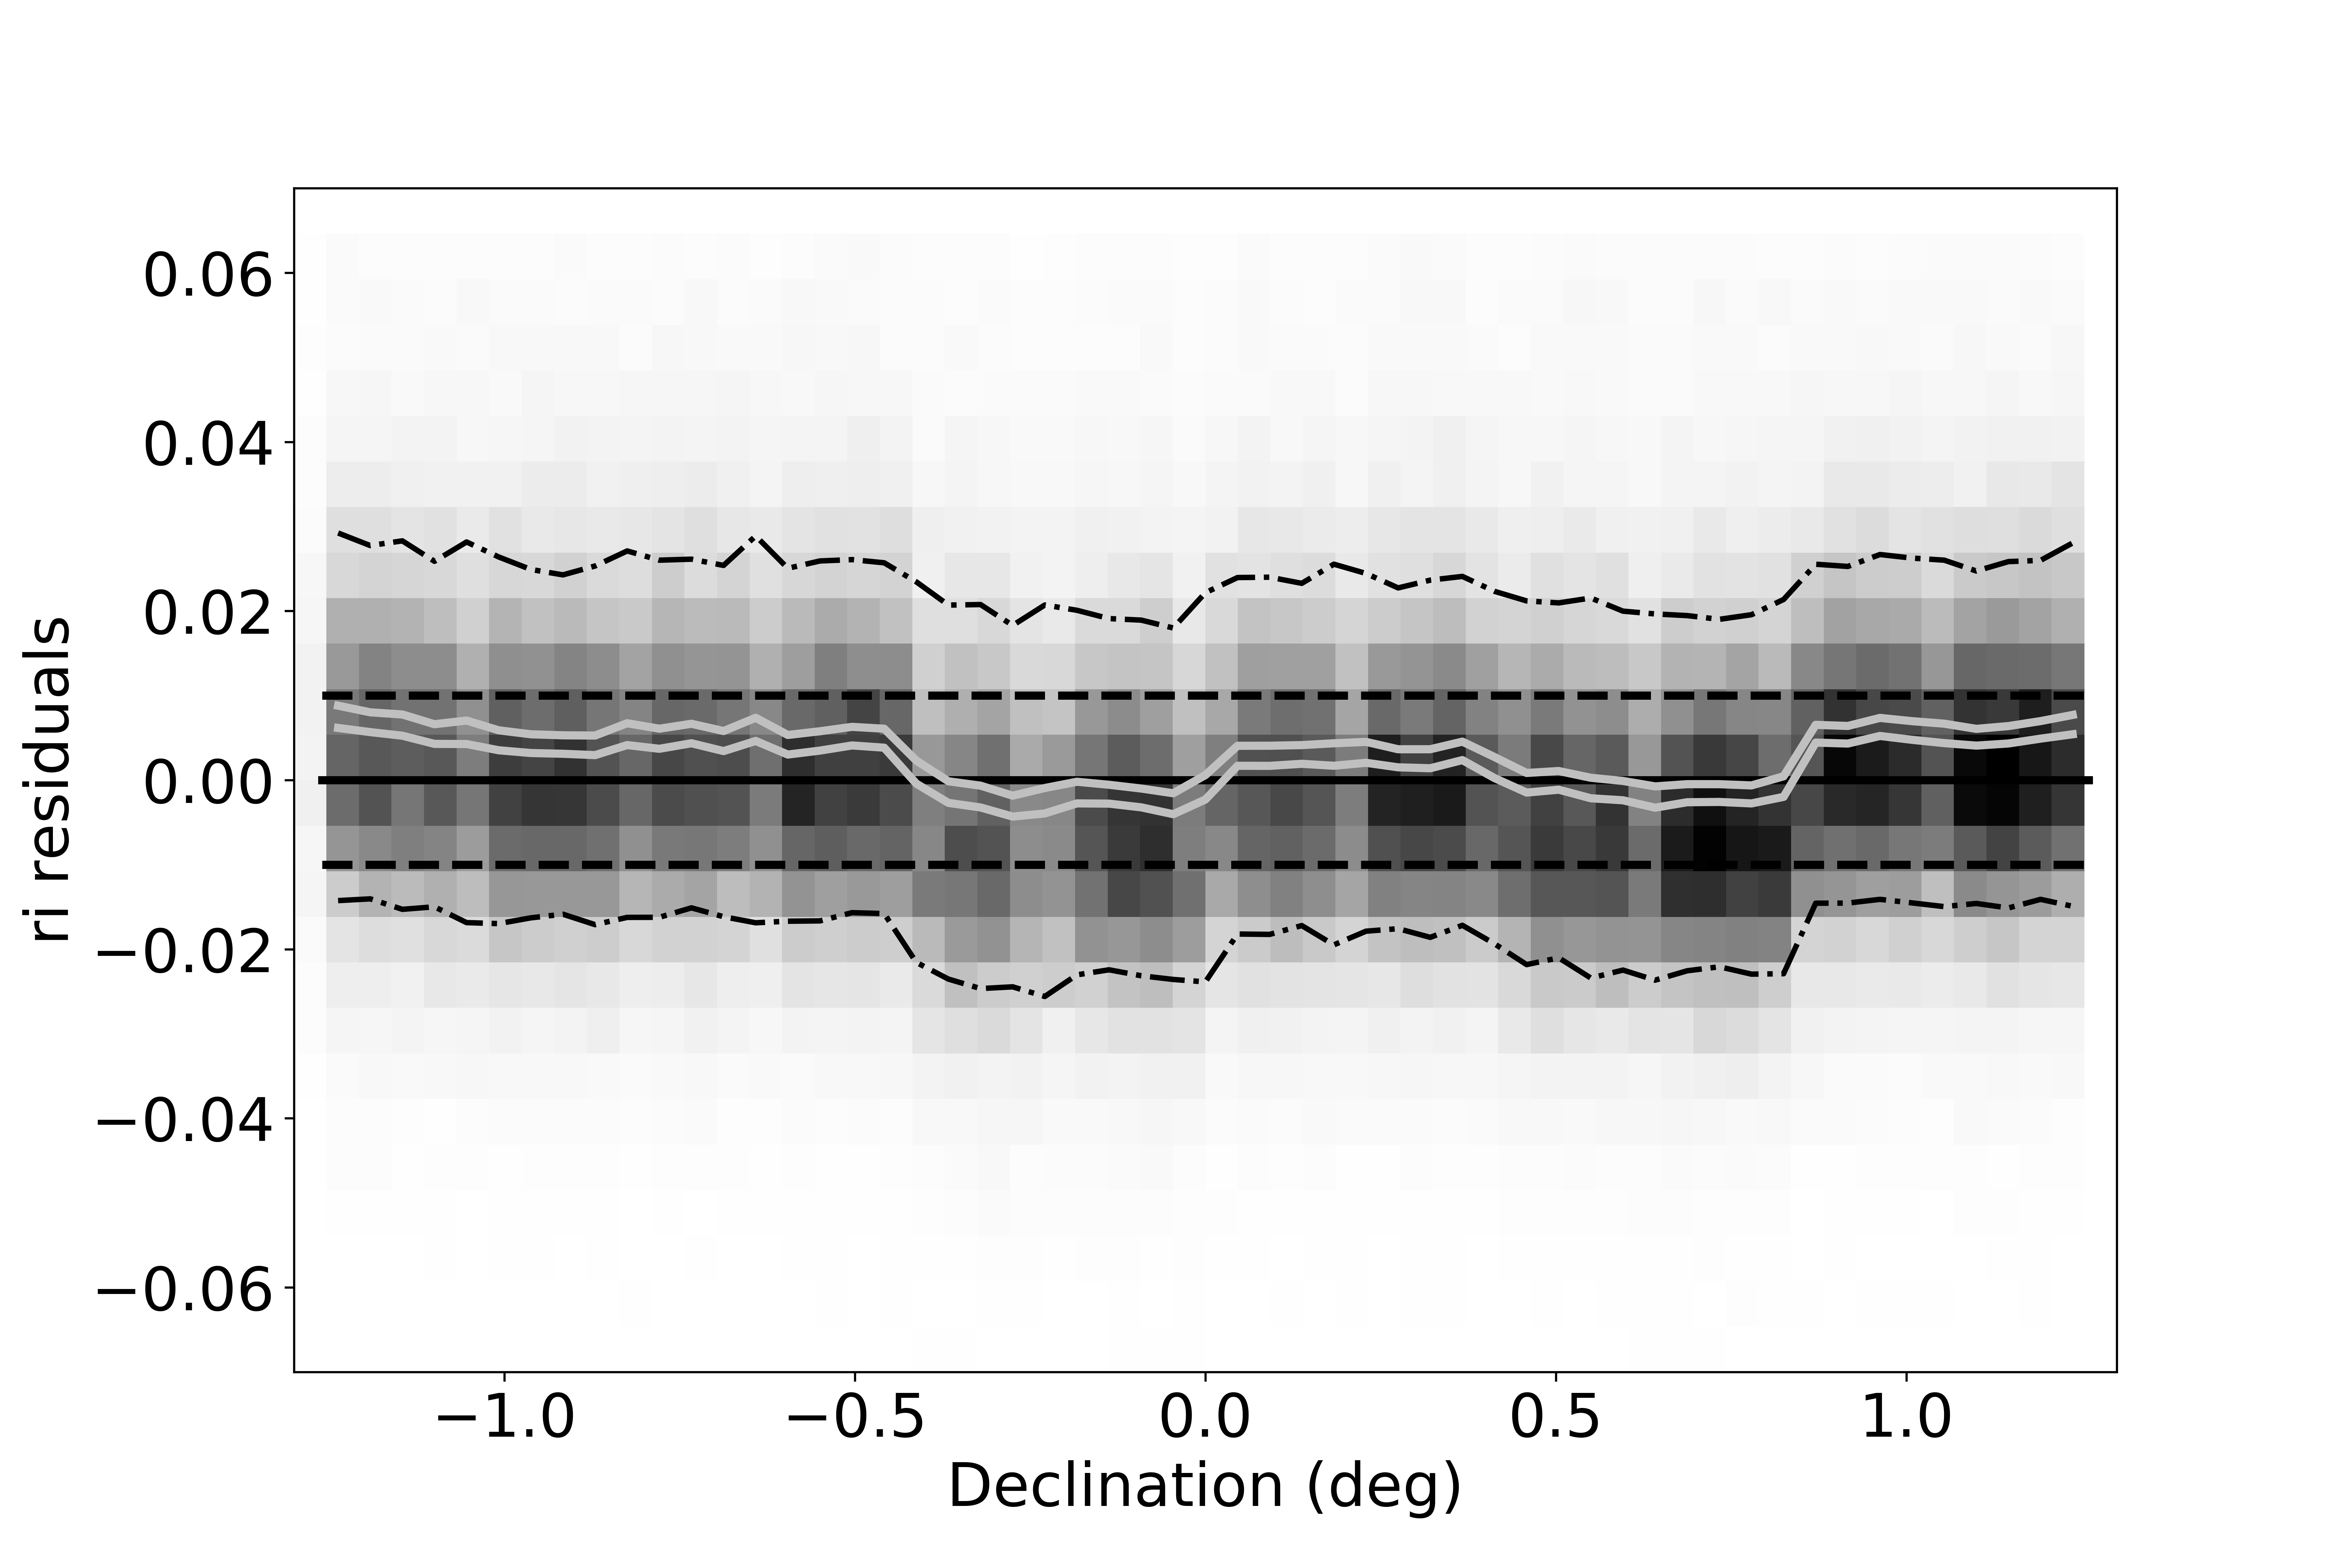
\includegraphics[width=9cm]{figures/colorResidGaiaColorsB_ri_Dec_Hess.png} 
\caption{Analogous to Figure~\ref{fig:graycorrDec}, except that here residuals 
correspond to differences between the SDSS $r-i$ color and a synthetic $r-i$ color
generated using Gaia's $BP-RP$ color. Note the signature of SDSS camera columns
at the level of a few millimags. The standard deviation for the binned medians is 
3.2 millimag (for other bands, please see Table~\ref{tab:GaiaRMS}.}
\label{fig:riresid}
\end{figure}


The largest corrections were derived for the $u$ band. Given that Gaia's BP-RP
color does not strongly constrain the $u$ band flux, we used the CFIS catalog 
(see Section~\ref{ssec:cfis}) as an independent verification test. We verified that
zeropoint errors in the SDSS catalog implied by Gaia's and CFIS data agree at the
level a few millimags in Declination direction, but found $\sim$0.01-0.02 mag
large inconsistencies for R.A. bins. For this reason, we only applied $u$ band 
correction in Declination direction. The plausible $u$ band zeropoint errors in 
the new catalog are further discussed in Section~\ref{sec:CFIStest}. This final 
catalog version was labeled v3.4, and it is also publicly available. 



\subsubsection{Validation of recalibration  \label{sec:SSCvsGaia}} 
  
By construction, the new v3.4 catalog should not show appreciable zeropoint residuals when 
binned by R.A. and Declination. We have verified this expectation for all colors used in 
recalibration. For illustration, Figure~\ref{fig:grVSgaiaRADec} shows such a test for the $g-r$ 
color, with binned median scatter of the order 1 millimag. 

\begin{figure}[th!]
    \centering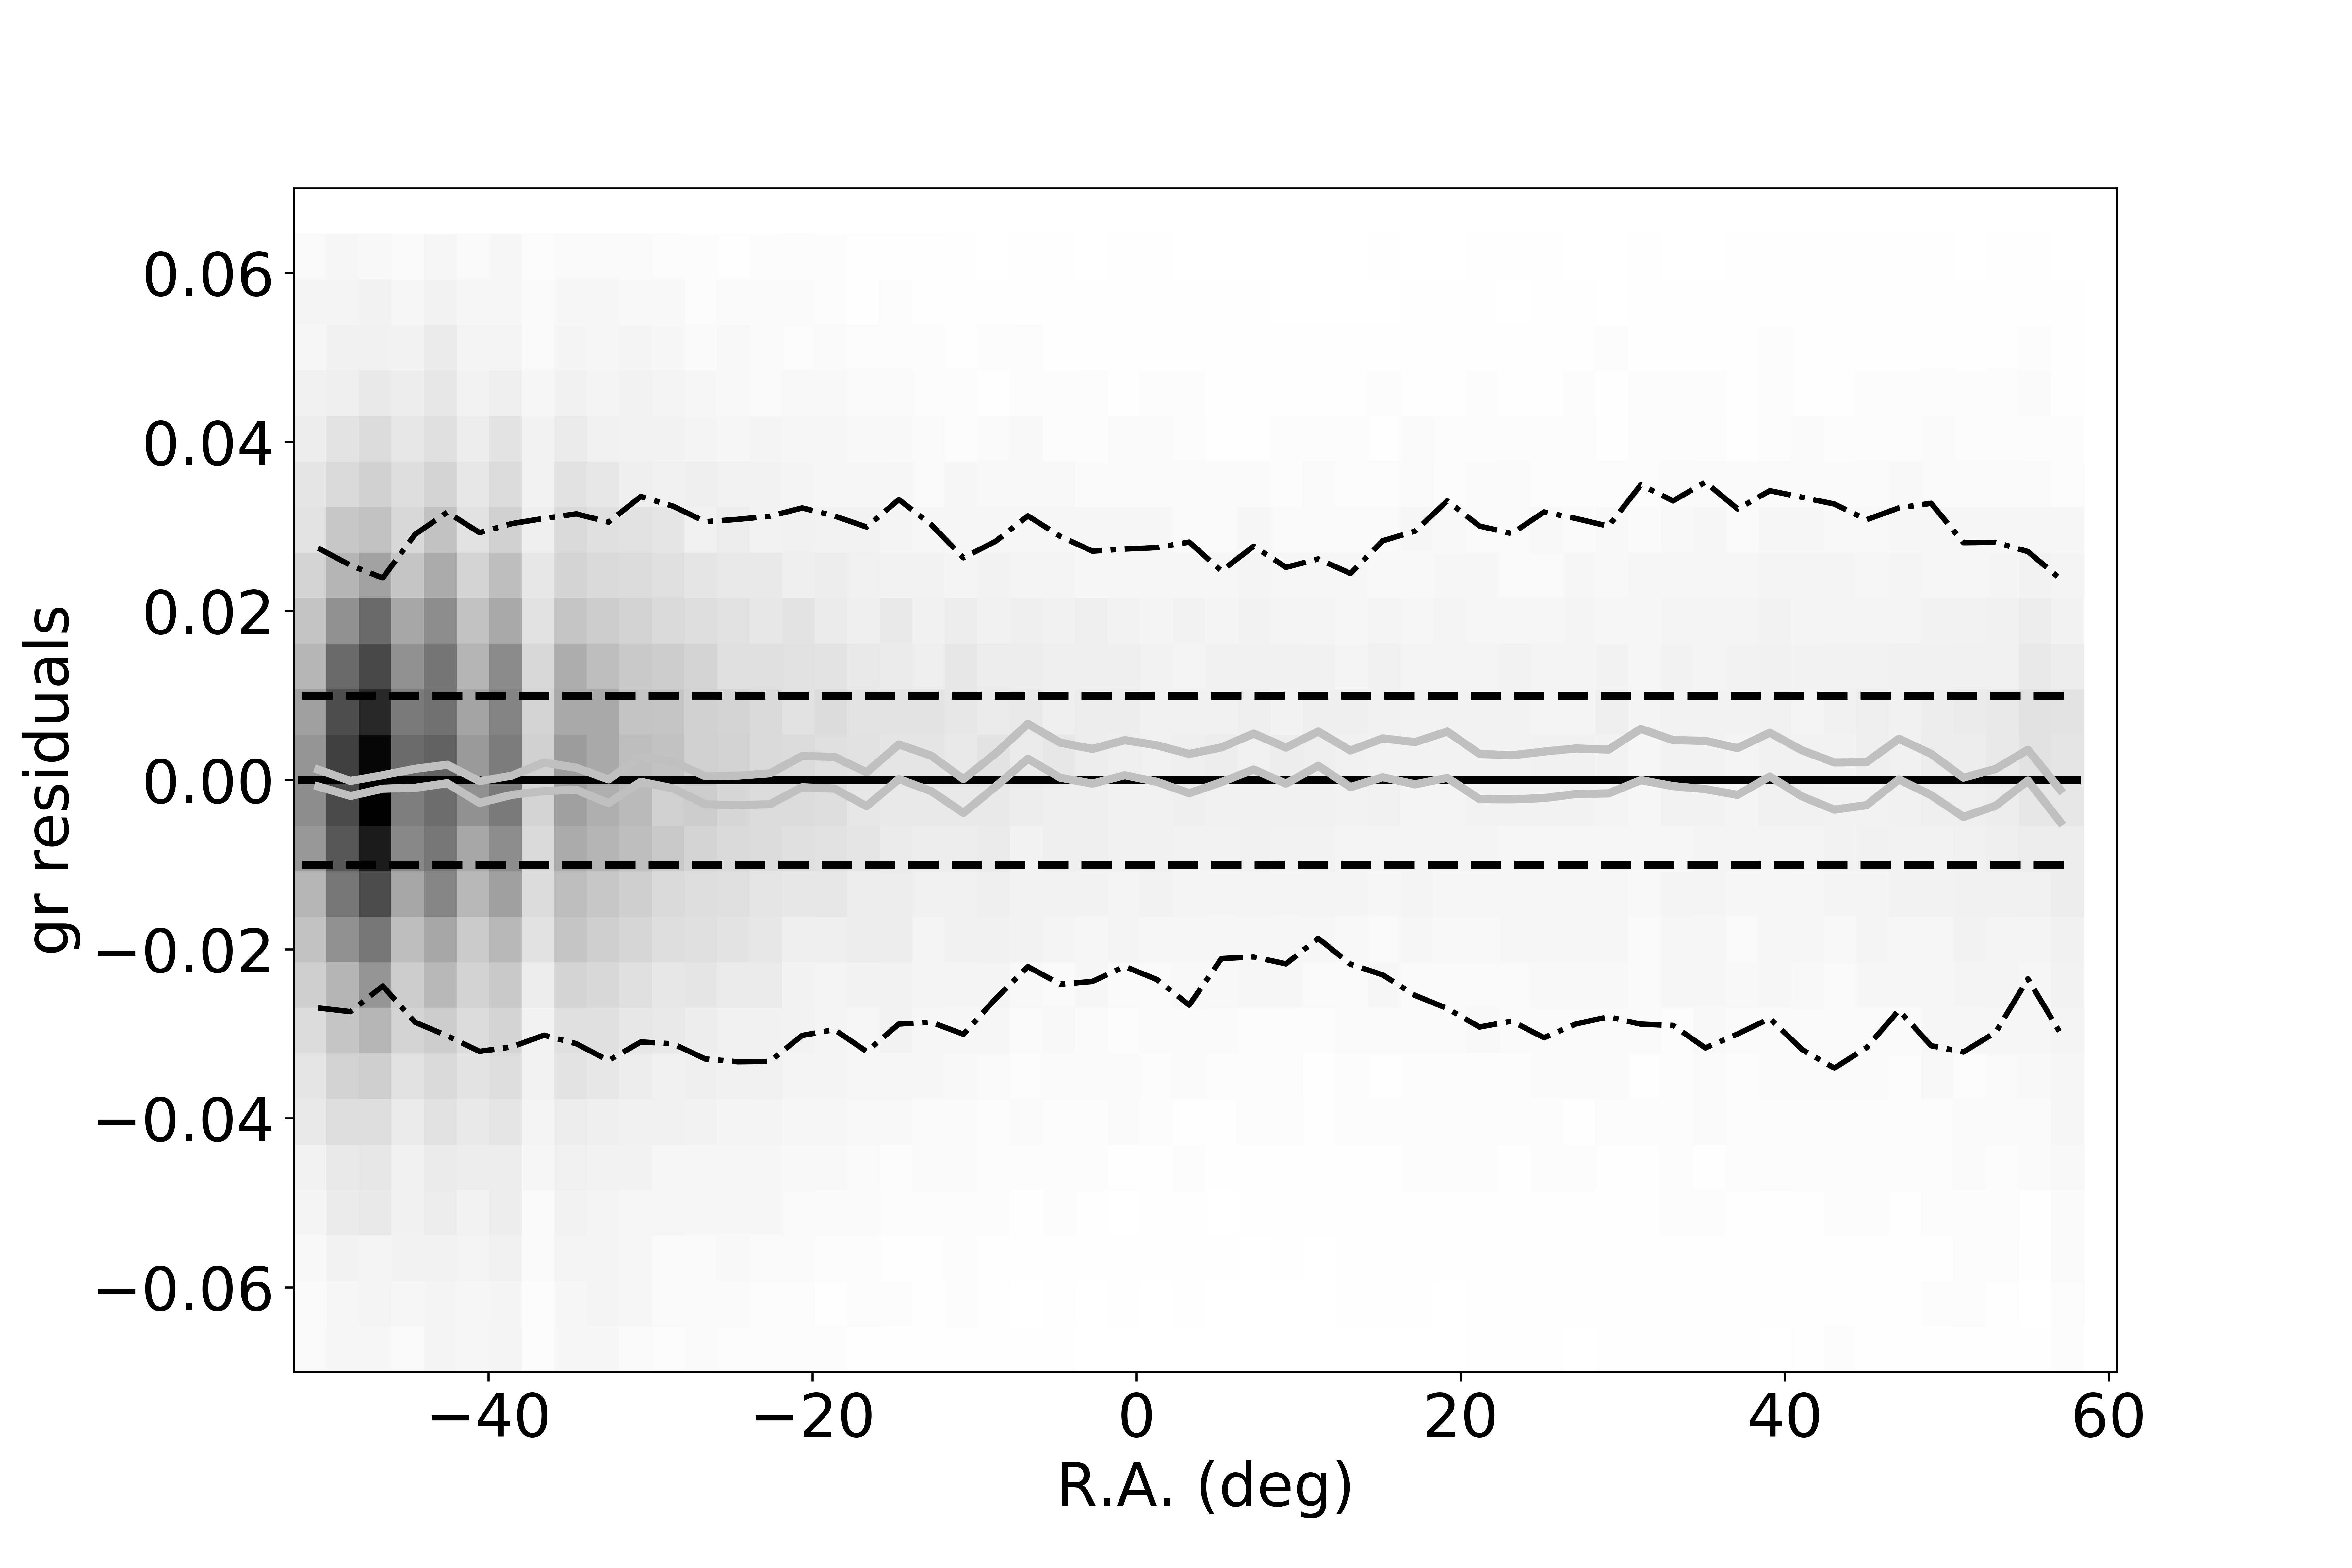
\includegraphics[width=7cm]{figures/colorResidGaiaColors_gr_RA_Hess.png} 
    \centering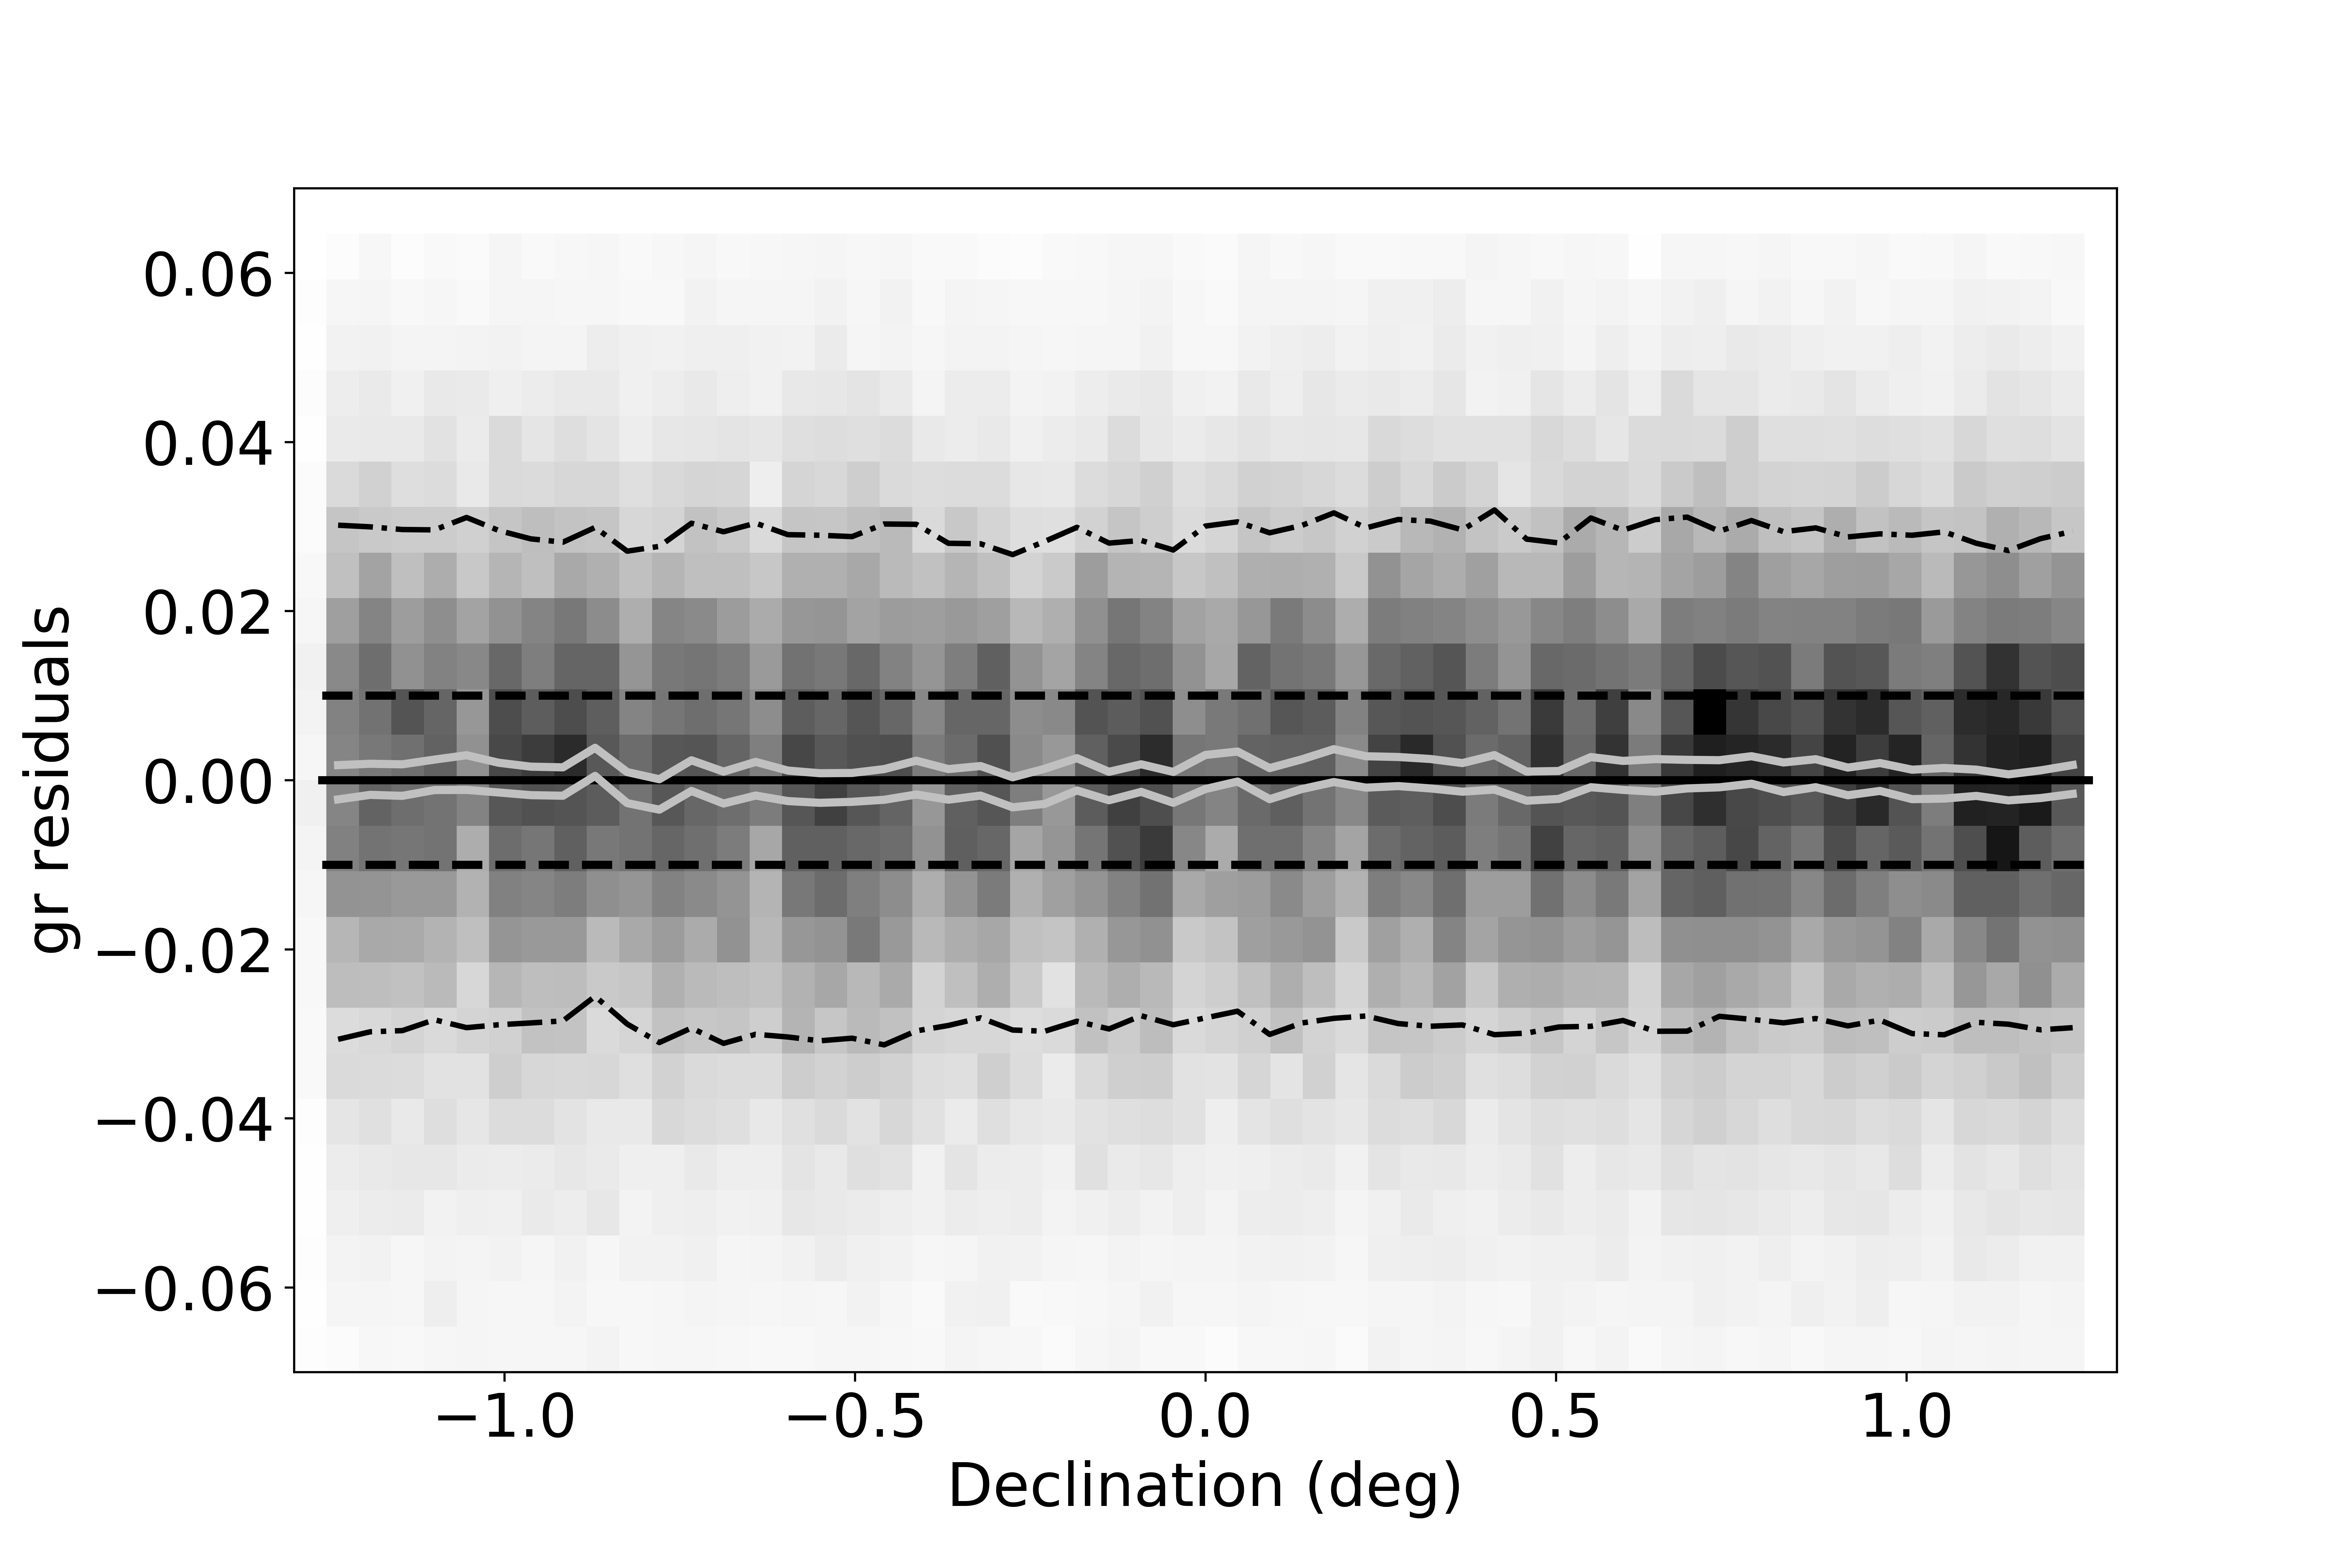
\includegraphics[width=7cm]{figures/colorResidGaiaColors_gr_Dec_Hess.png} 
\caption{Left: analogous to Figure~\ref{fig:graycorrRA}, except that here residuals between
the SDSS $g-r$ color from the v3.4 catalog and a synthetic $g-r$ color generated using 
Gaia's $BP-RP$ color are shown. The binned median scatter is 1.6 millimag. Right: the 
$g-r$ residuals are shown as a function of Declination. The binned median scatter is 
0.8 millimag.}
\label{fig:grVSgaiaRADec}
\end{figure}
 

\subsection{Comparison of the SDSS v2.6 and v3.4 catalogs \label{sec:v26v34}} 
 
The v2.6 (``old'') SDSS Standard Star Catalog has been extensively used 
\citep[e.g.,][]{2008AJ....135..338F},
and here we briefly analyze differences between the v3.4 (``new'') and v2.6 magnitudes
to inform the future users about catalog consistency. 
In our analysis, we first compare v2.6 and v3.4 magnitudes of individual stars and 
bin the differences by R.A., Declination and magnitude. 

On average, both catalog versions are on the same magnitude scale (the median $ugriz$ 
magnitude differences for all stars are zero by construction). There are no systematic offsets 
when binned by magnitude, as illustrated in Figure~\ref{fig:v26v34drr}. The most obvious 
differences appear when magnitude differences are binned by Declination. An example is 
shown in Figure~\ref{fig:v26v34drDec}, where the periodicity of residuals corresponds to the 
field-of-view size for the SDSS Photometric Telescope \citep{2006AN....327..821T}. 
The standard deviation for median values per bin is 6.8 millimag, with extreme values about 
0.01 mag. It is likely that systematic errors in the calibration star network photometry 
were propagated through ``flat-field corrections'' discussed by \pO\ to the v2.6 catalog.
We note that these errors, now found thanks to Gaia catalogs, are well within the claimed
photemetric accuracy by both \pO\ and \cite{2002AJ....123.2121S}. The standard deviation 
for median values per bin for all bands and both coordinates is listed in Table~\ref{tab:oldnewRMS}. 


\begin{deluxetable}{l|c|c}[ht!]
\tablecaption{The robust standard deviation for magnitude differences between the v2.6 (old)
and v3.4 (new) catalogs. \label{tab:oldnewRMS}}
\tablehead{
\colhead{Band} & \colhead{rms for R.A.} & \colhead{rms for Dec}
}
\startdata
       $u$        &        2.3$^a$    &    25.5      \\
       $g$        &        4.5    &      9.4      \\  
       $r$         &        2.0    &      7.0      \\  
       $i$         &        5.3    &      6.5      \\ 
       $z$        &        8.9    &      8.4      \\ 
\enddata
\tablenotetext{a}{For the $u$ band, the scatter in R.A. direction is due to more observations
in v3.4 than in v2.6, rather than zeropoint correction.} 
\end{deluxetable}
   


\begin{figure}[th!]
    \centering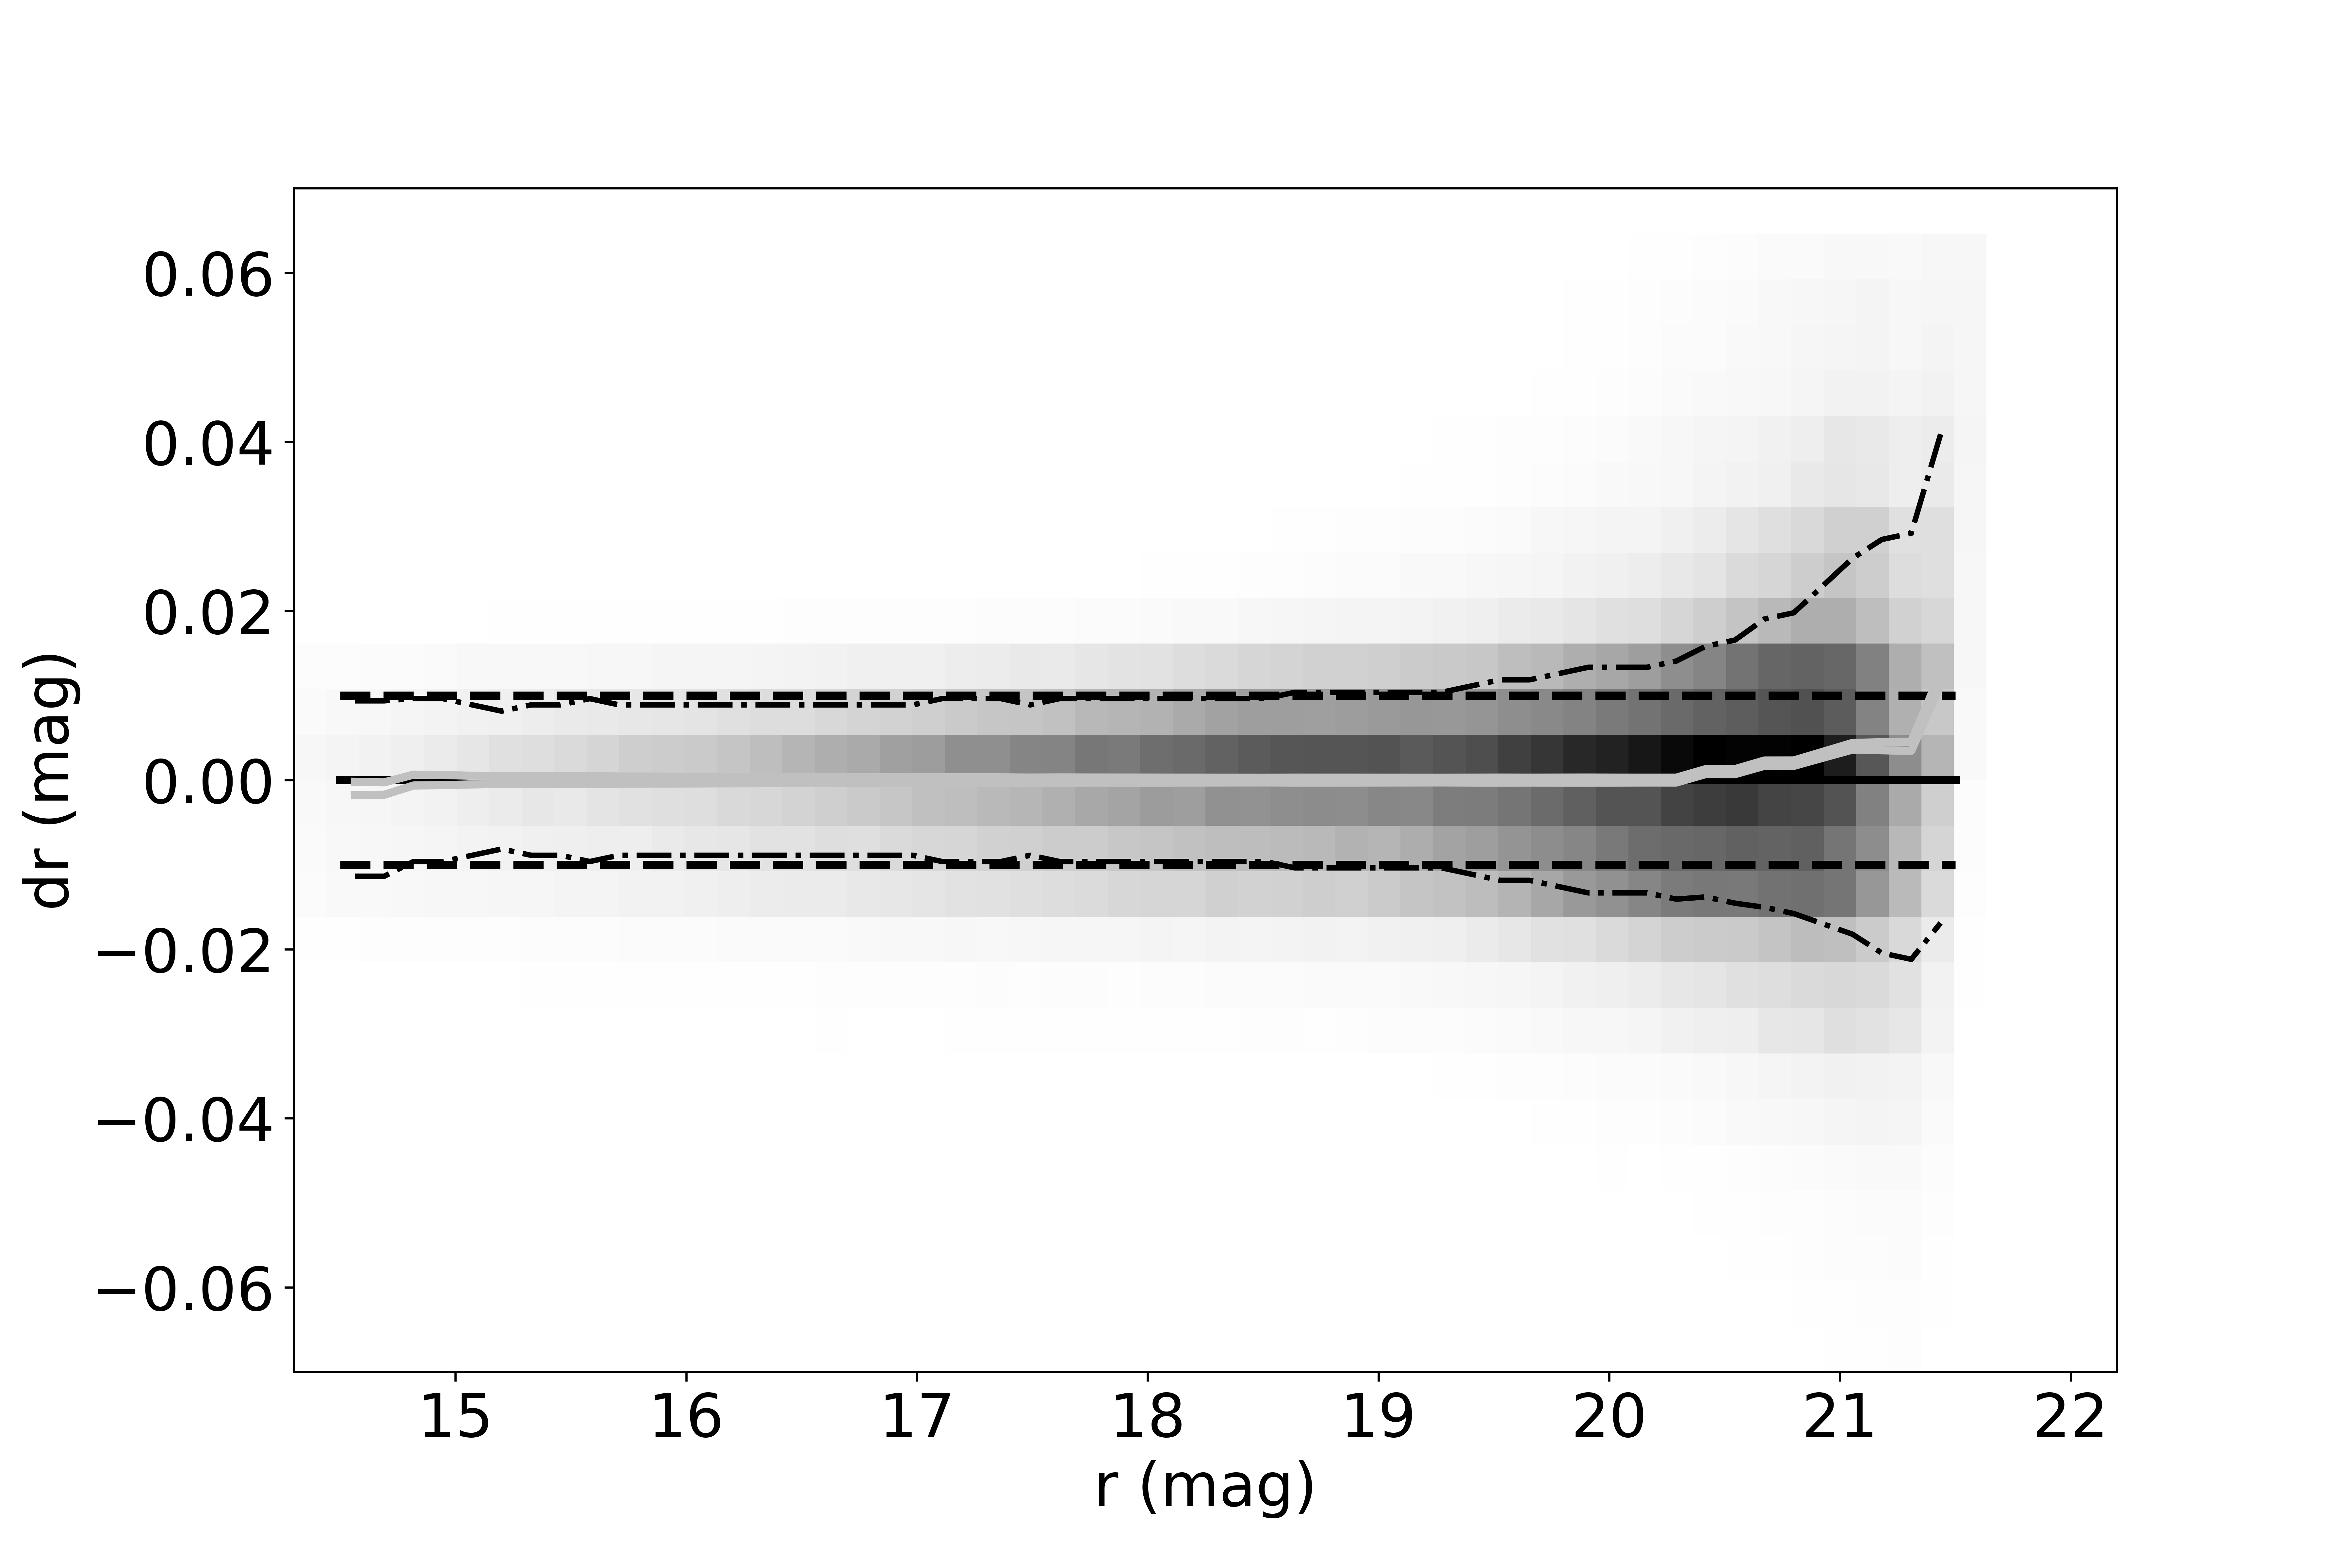
\includegraphics[width=9cm]{figures/testV26vsV33_r_dr_r_mag_Hess.png} 
\caption{Analogous to Figure~\ref{fig:v26v34drDec}, except that here the $r$ band
differences are shown as a function of the $r$ band magnitude. The scatted of median
values per bin is 1.9 millimag. The scatter of individual values is $\sim0.01$ mag
for $r<20$, and it is due to more data in the new catalog.} 
\label{fig:v26v34drr}
\end{figure}


\begin{figure}[th!]
    \centering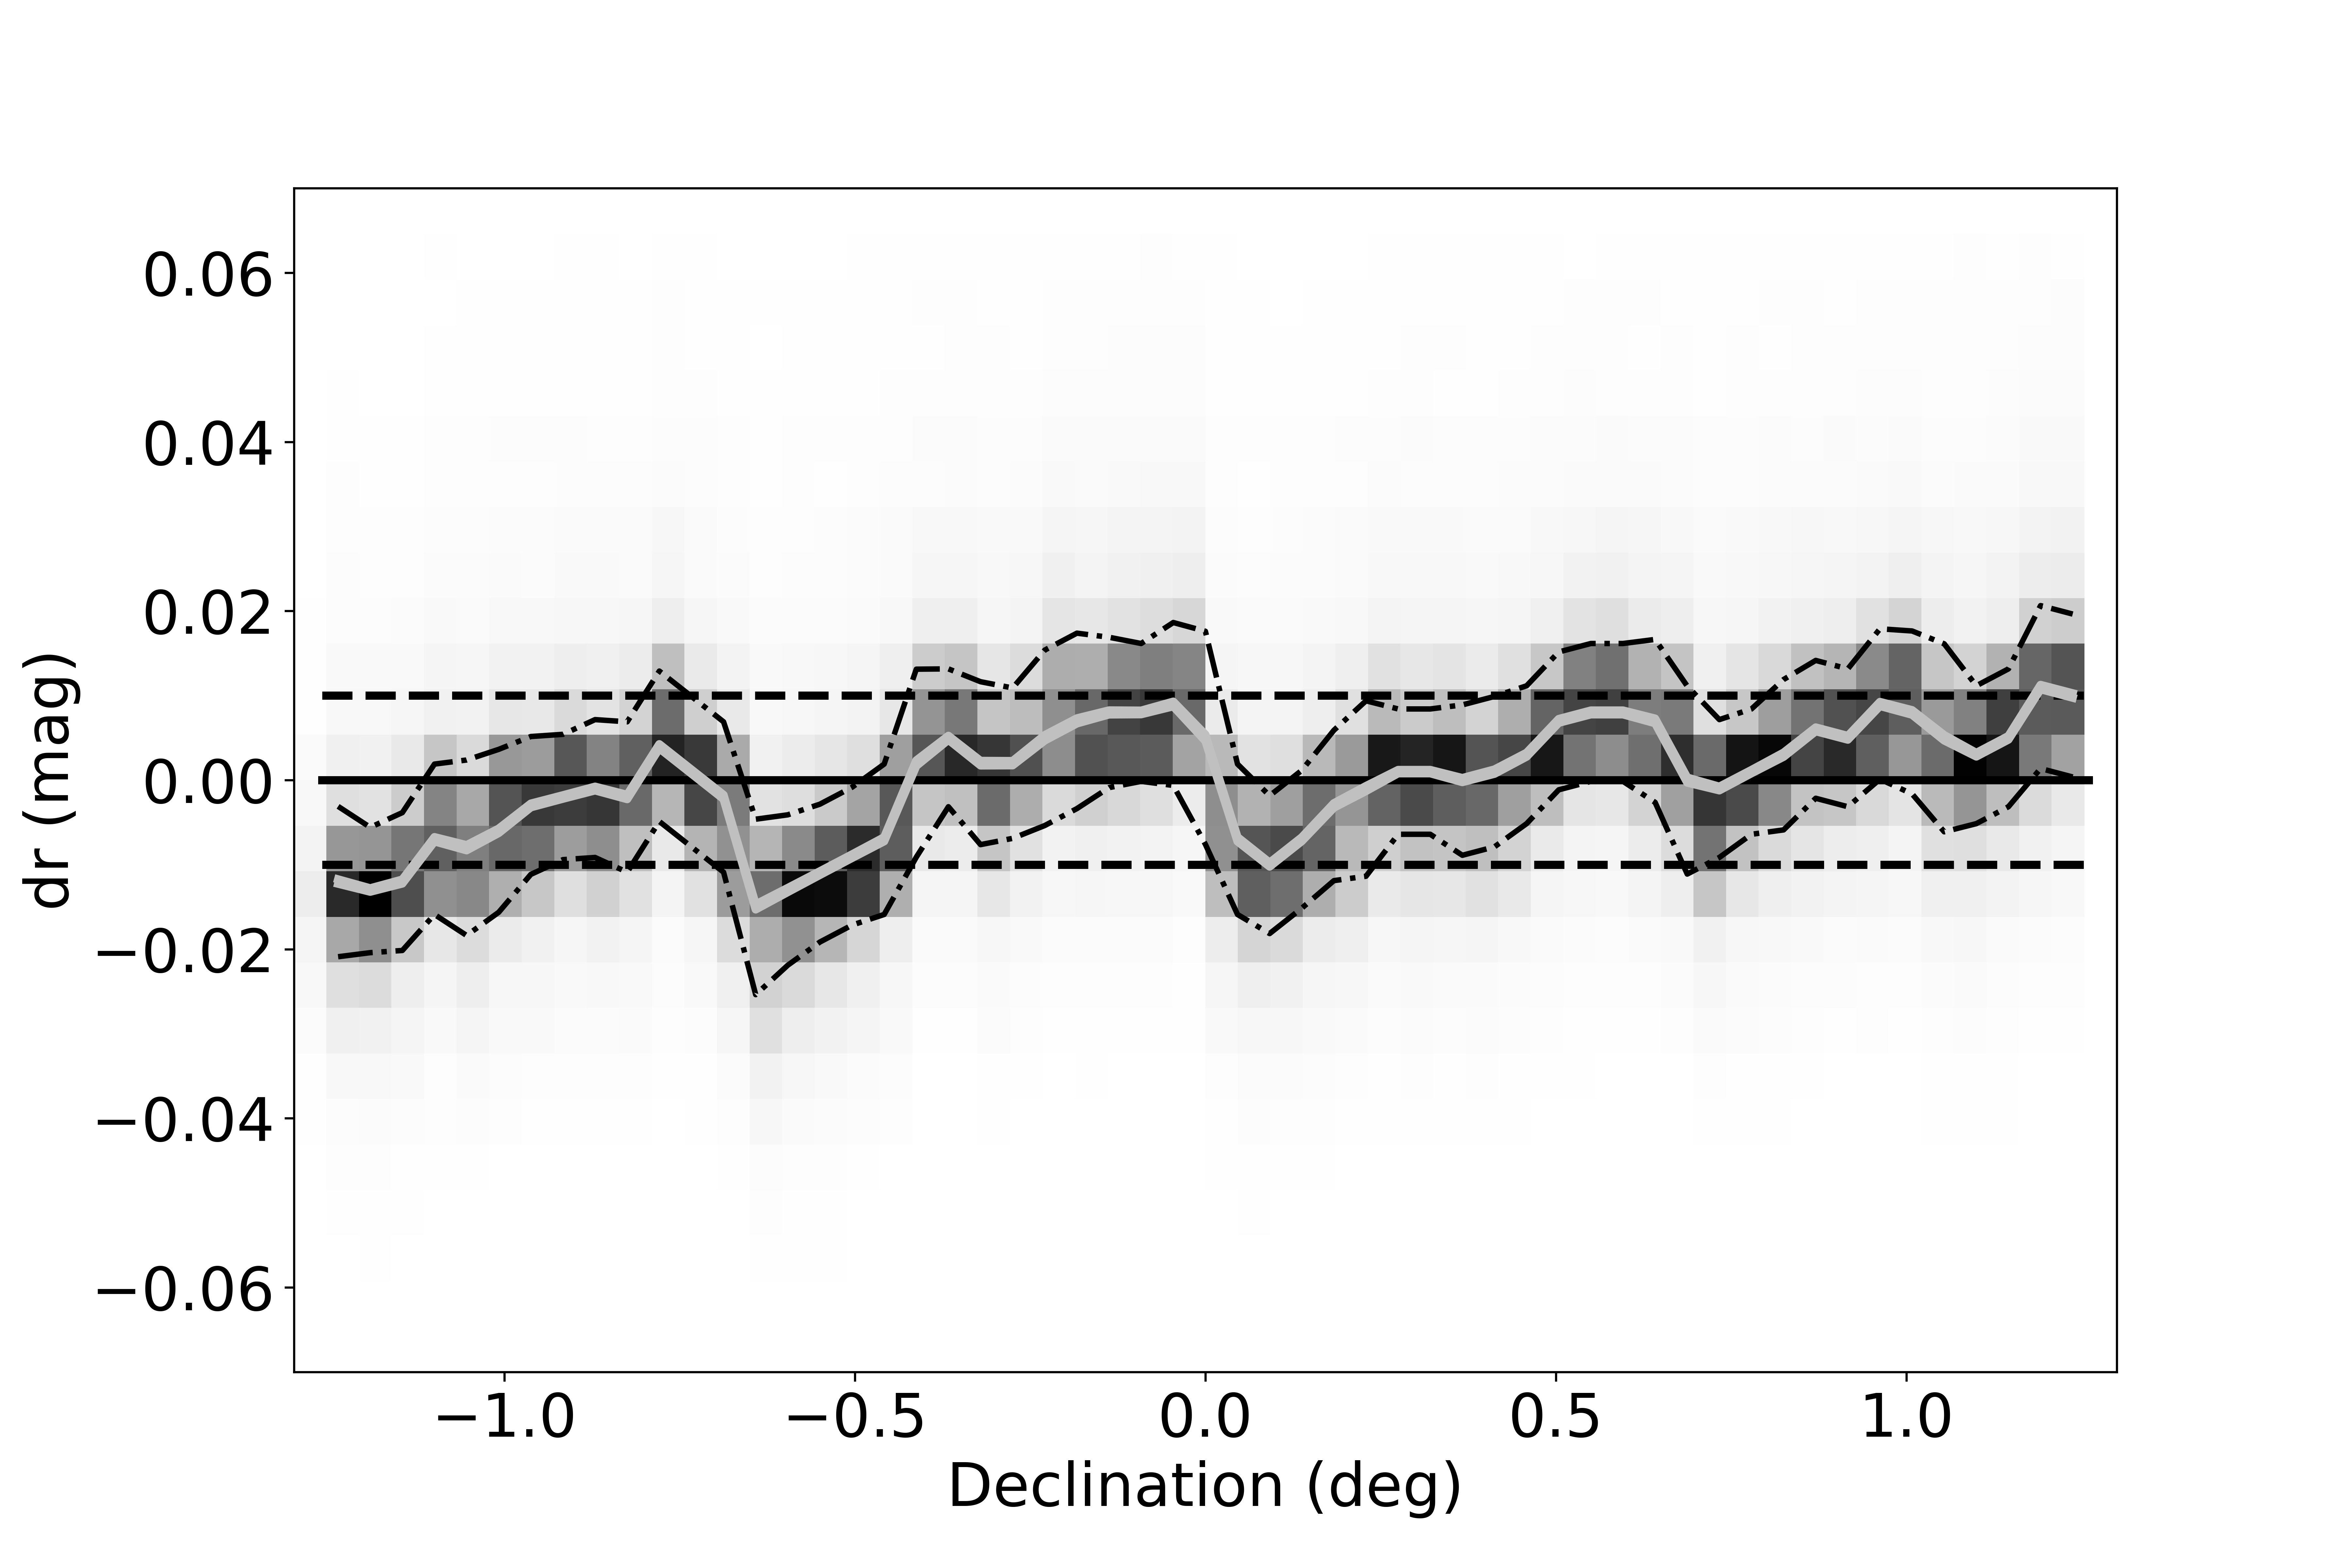
\includegraphics[width=9cm]{figures/testV26vsV33_r_dr_Dec_Hess.png} 
\caption{The differences between $r$ band magnitudes listed in the v2.6 and v3.4 
    SDSS Standard Star catalogs. The size of the four regions corresponds to the
field-of-view size of the SDSS Photometric Telescope. The standard 
deviation for median values per bin is 6.8 millimag, with extreme values about 0.01 mag. 
The scatter of binned medians in R.A. direction is much smaller -- 2.0 millimag. 
For statistics in other bands, please see Table~\ref{tab:oldnewRMS}.}
\label{fig:v26v34drDec}
\end{figure}
 


Given the quality of Gaia photometry, there should be no doubt that SDSS $ugriz$ photometry
reported in the new v.3.4 catalog is superior to the old v2.6 catalog. Nevertheless, we perform
additional tests, based on the position of the stellar locus in the $g-r$ vs. $u-g$, $r-i$ vs. $g-r$ 
and $i-z$ vs. $r-i$ color-color diagrams  \citep{2004AN....325..583I}. The tests are based
on the second principal color for the blue part of the stellar locus, whose median should 
not deviate from zero by construction. Figure~\ref{fig:comparew} compares the behavior
of the $w$ color for the old v2.6 and new v3.4 catalog and demonstrates that the $gri$
photometry is better calibrated in the latter. The behavior of the $s$ and $y$ colors for the 
new catalog is shown in Figure~\ref{fig:comparesy}. {\it Based on these tests, we find that 
the contribution of the zeropoint errors is $<5$ millimag to $gri$ photometry, and 
$<10$ millimag for the $u$ and $z$ bands.} 



\begin{figure}[th!]
    \centering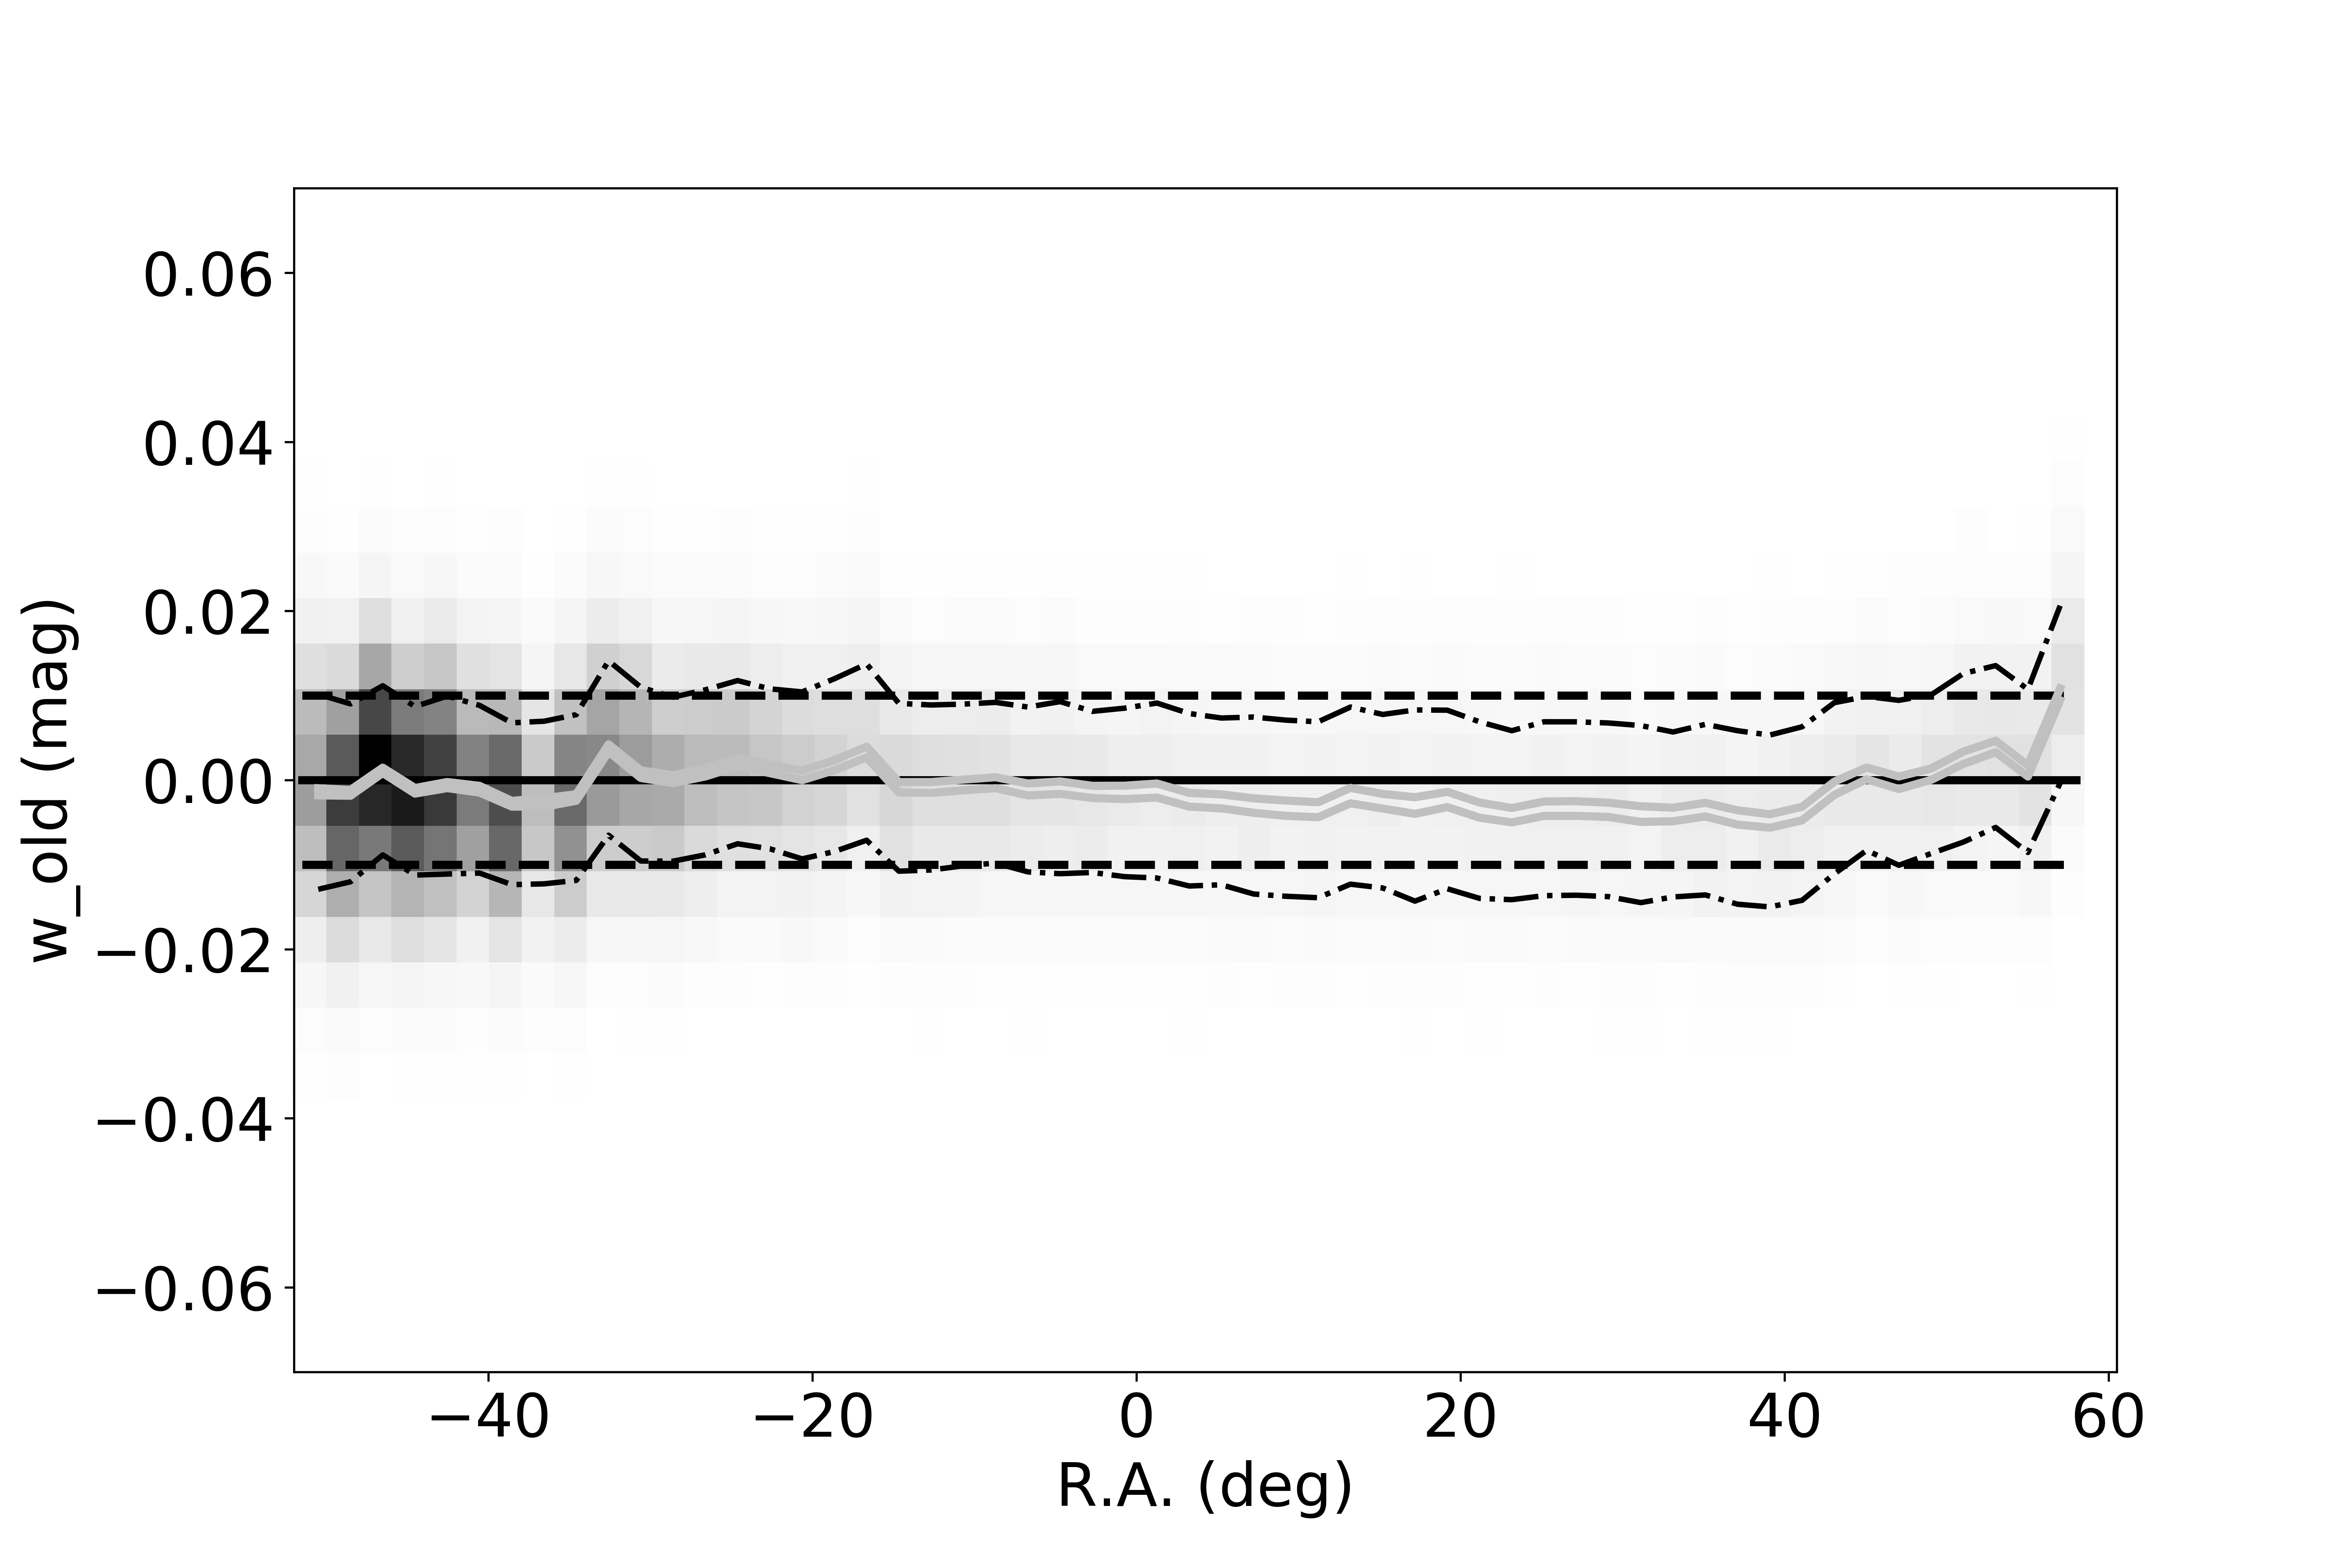
\includegraphics[width=7cm]{figures/testV26vsV33_r_w_old_RA_Hess.png}
    \centering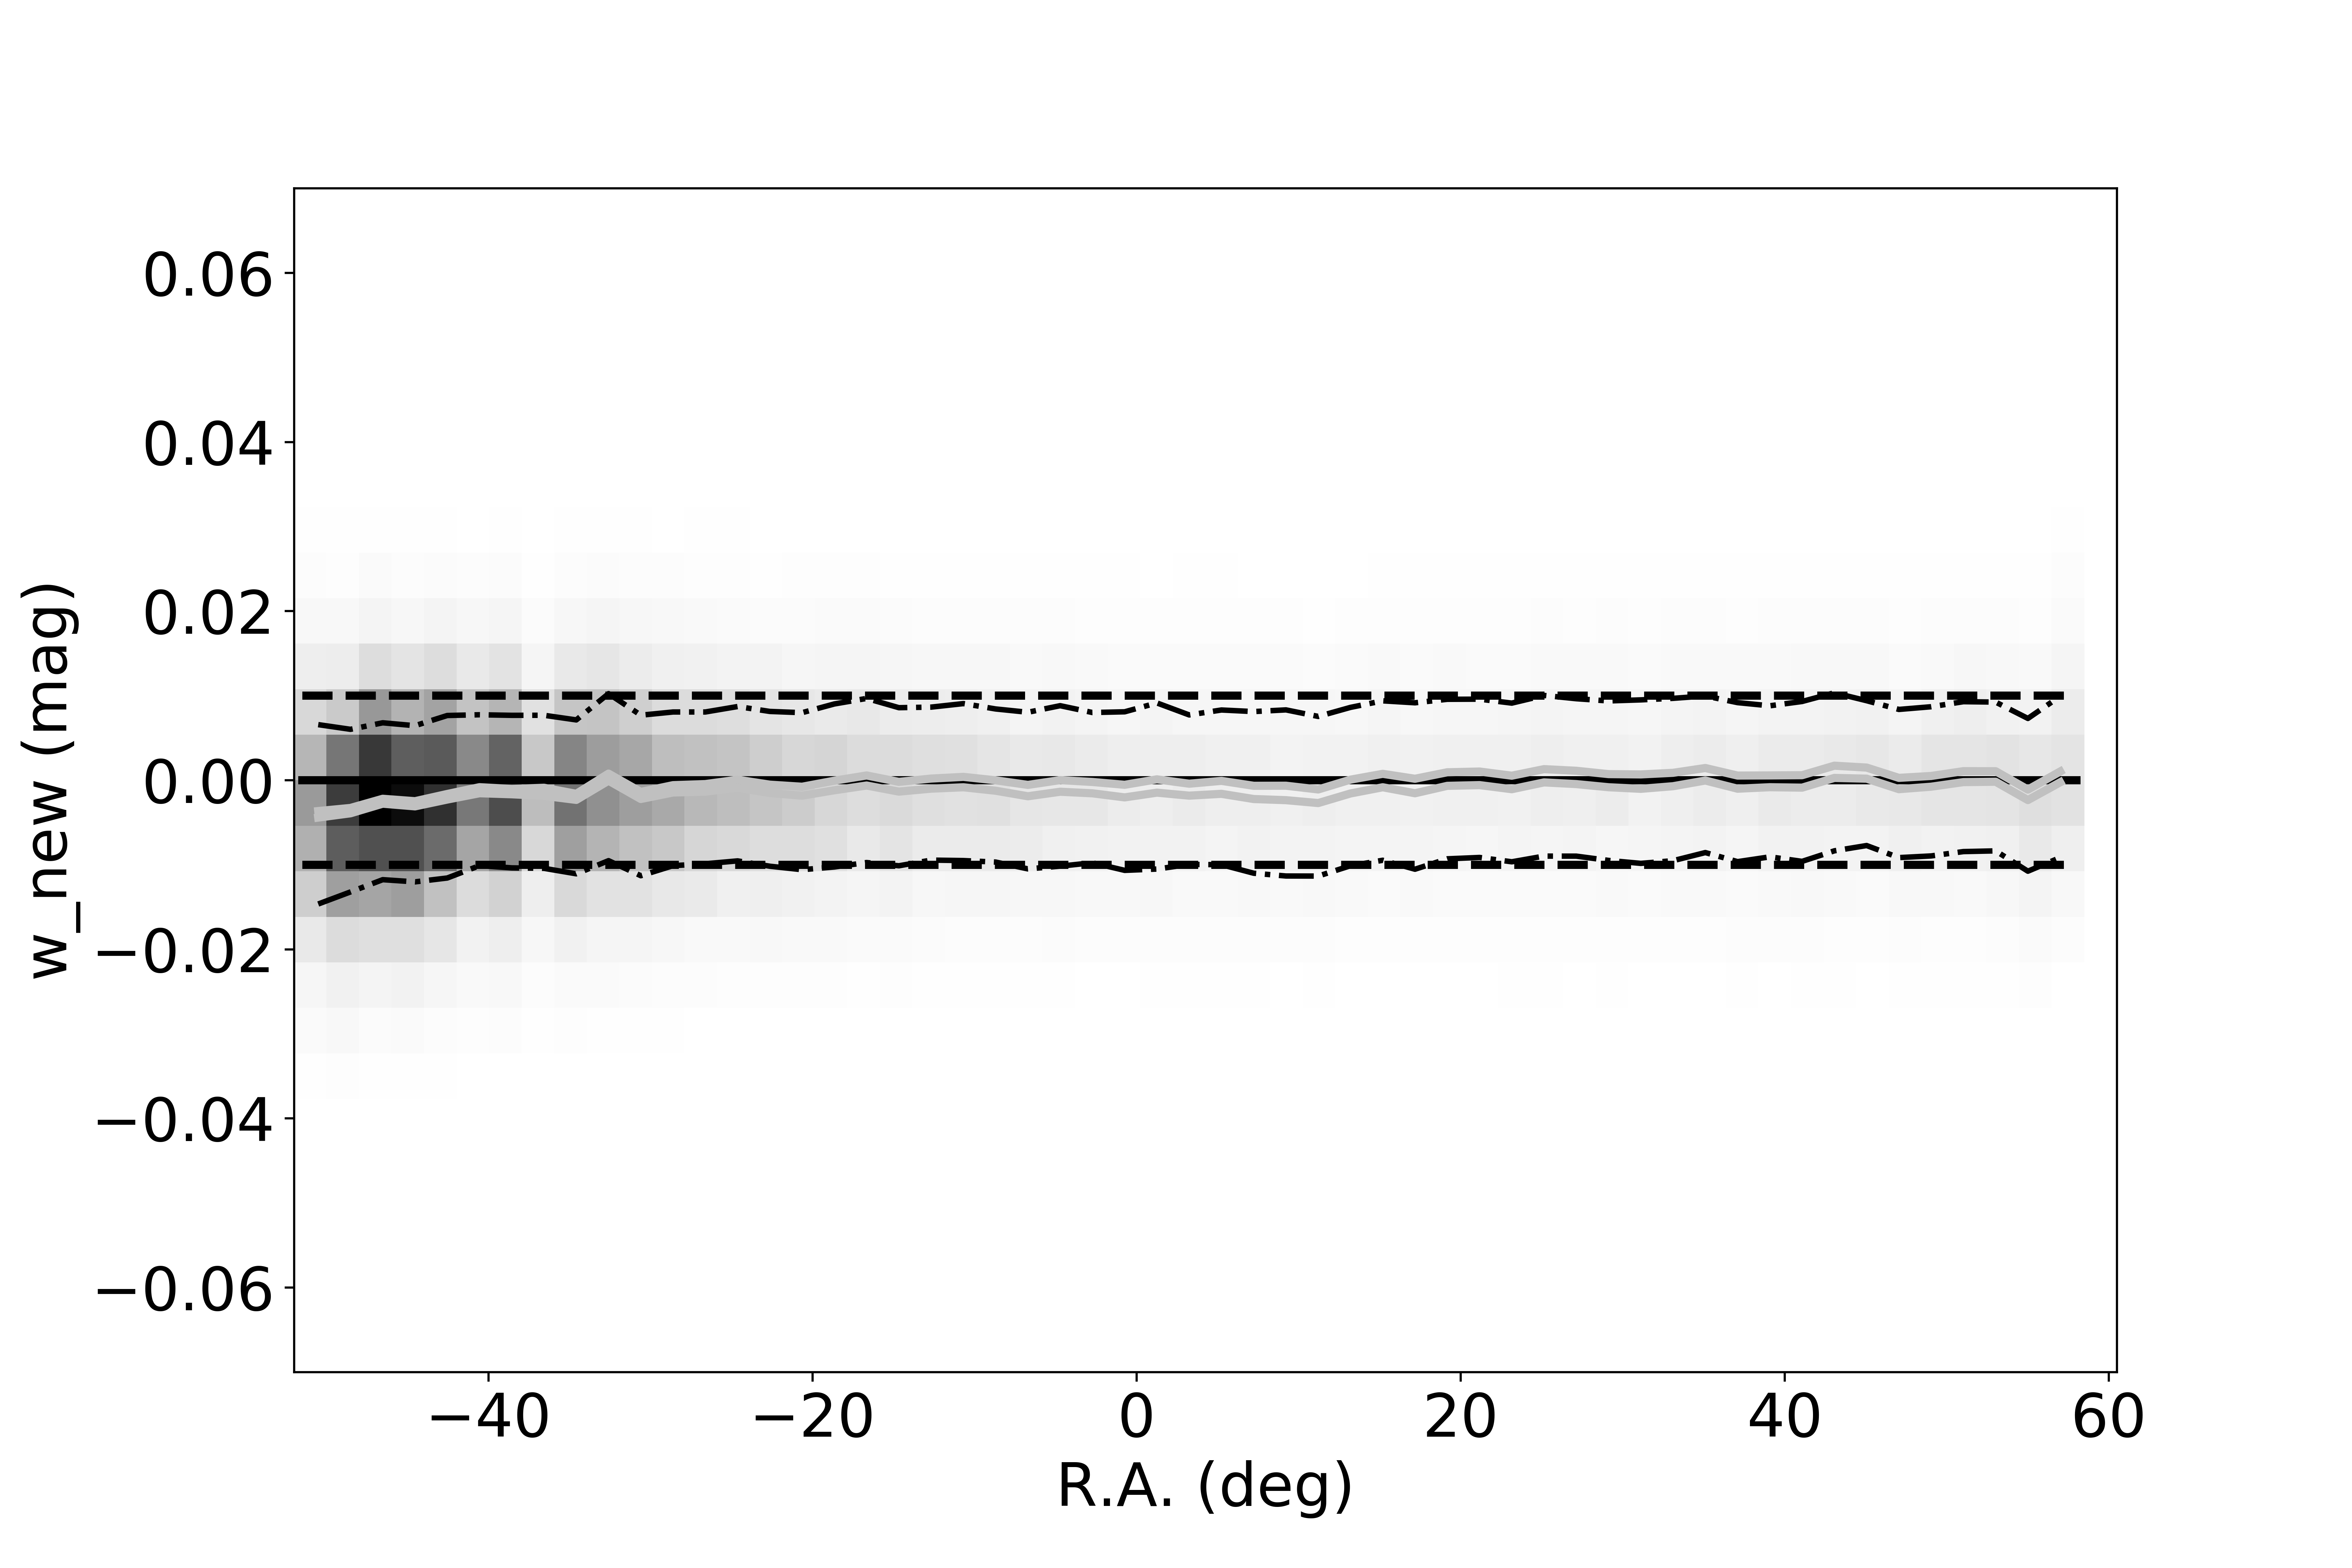
\includegraphics[width=7cm]{figures/testV26vsV33_r_w_new_RA_Hess.png}
    \centering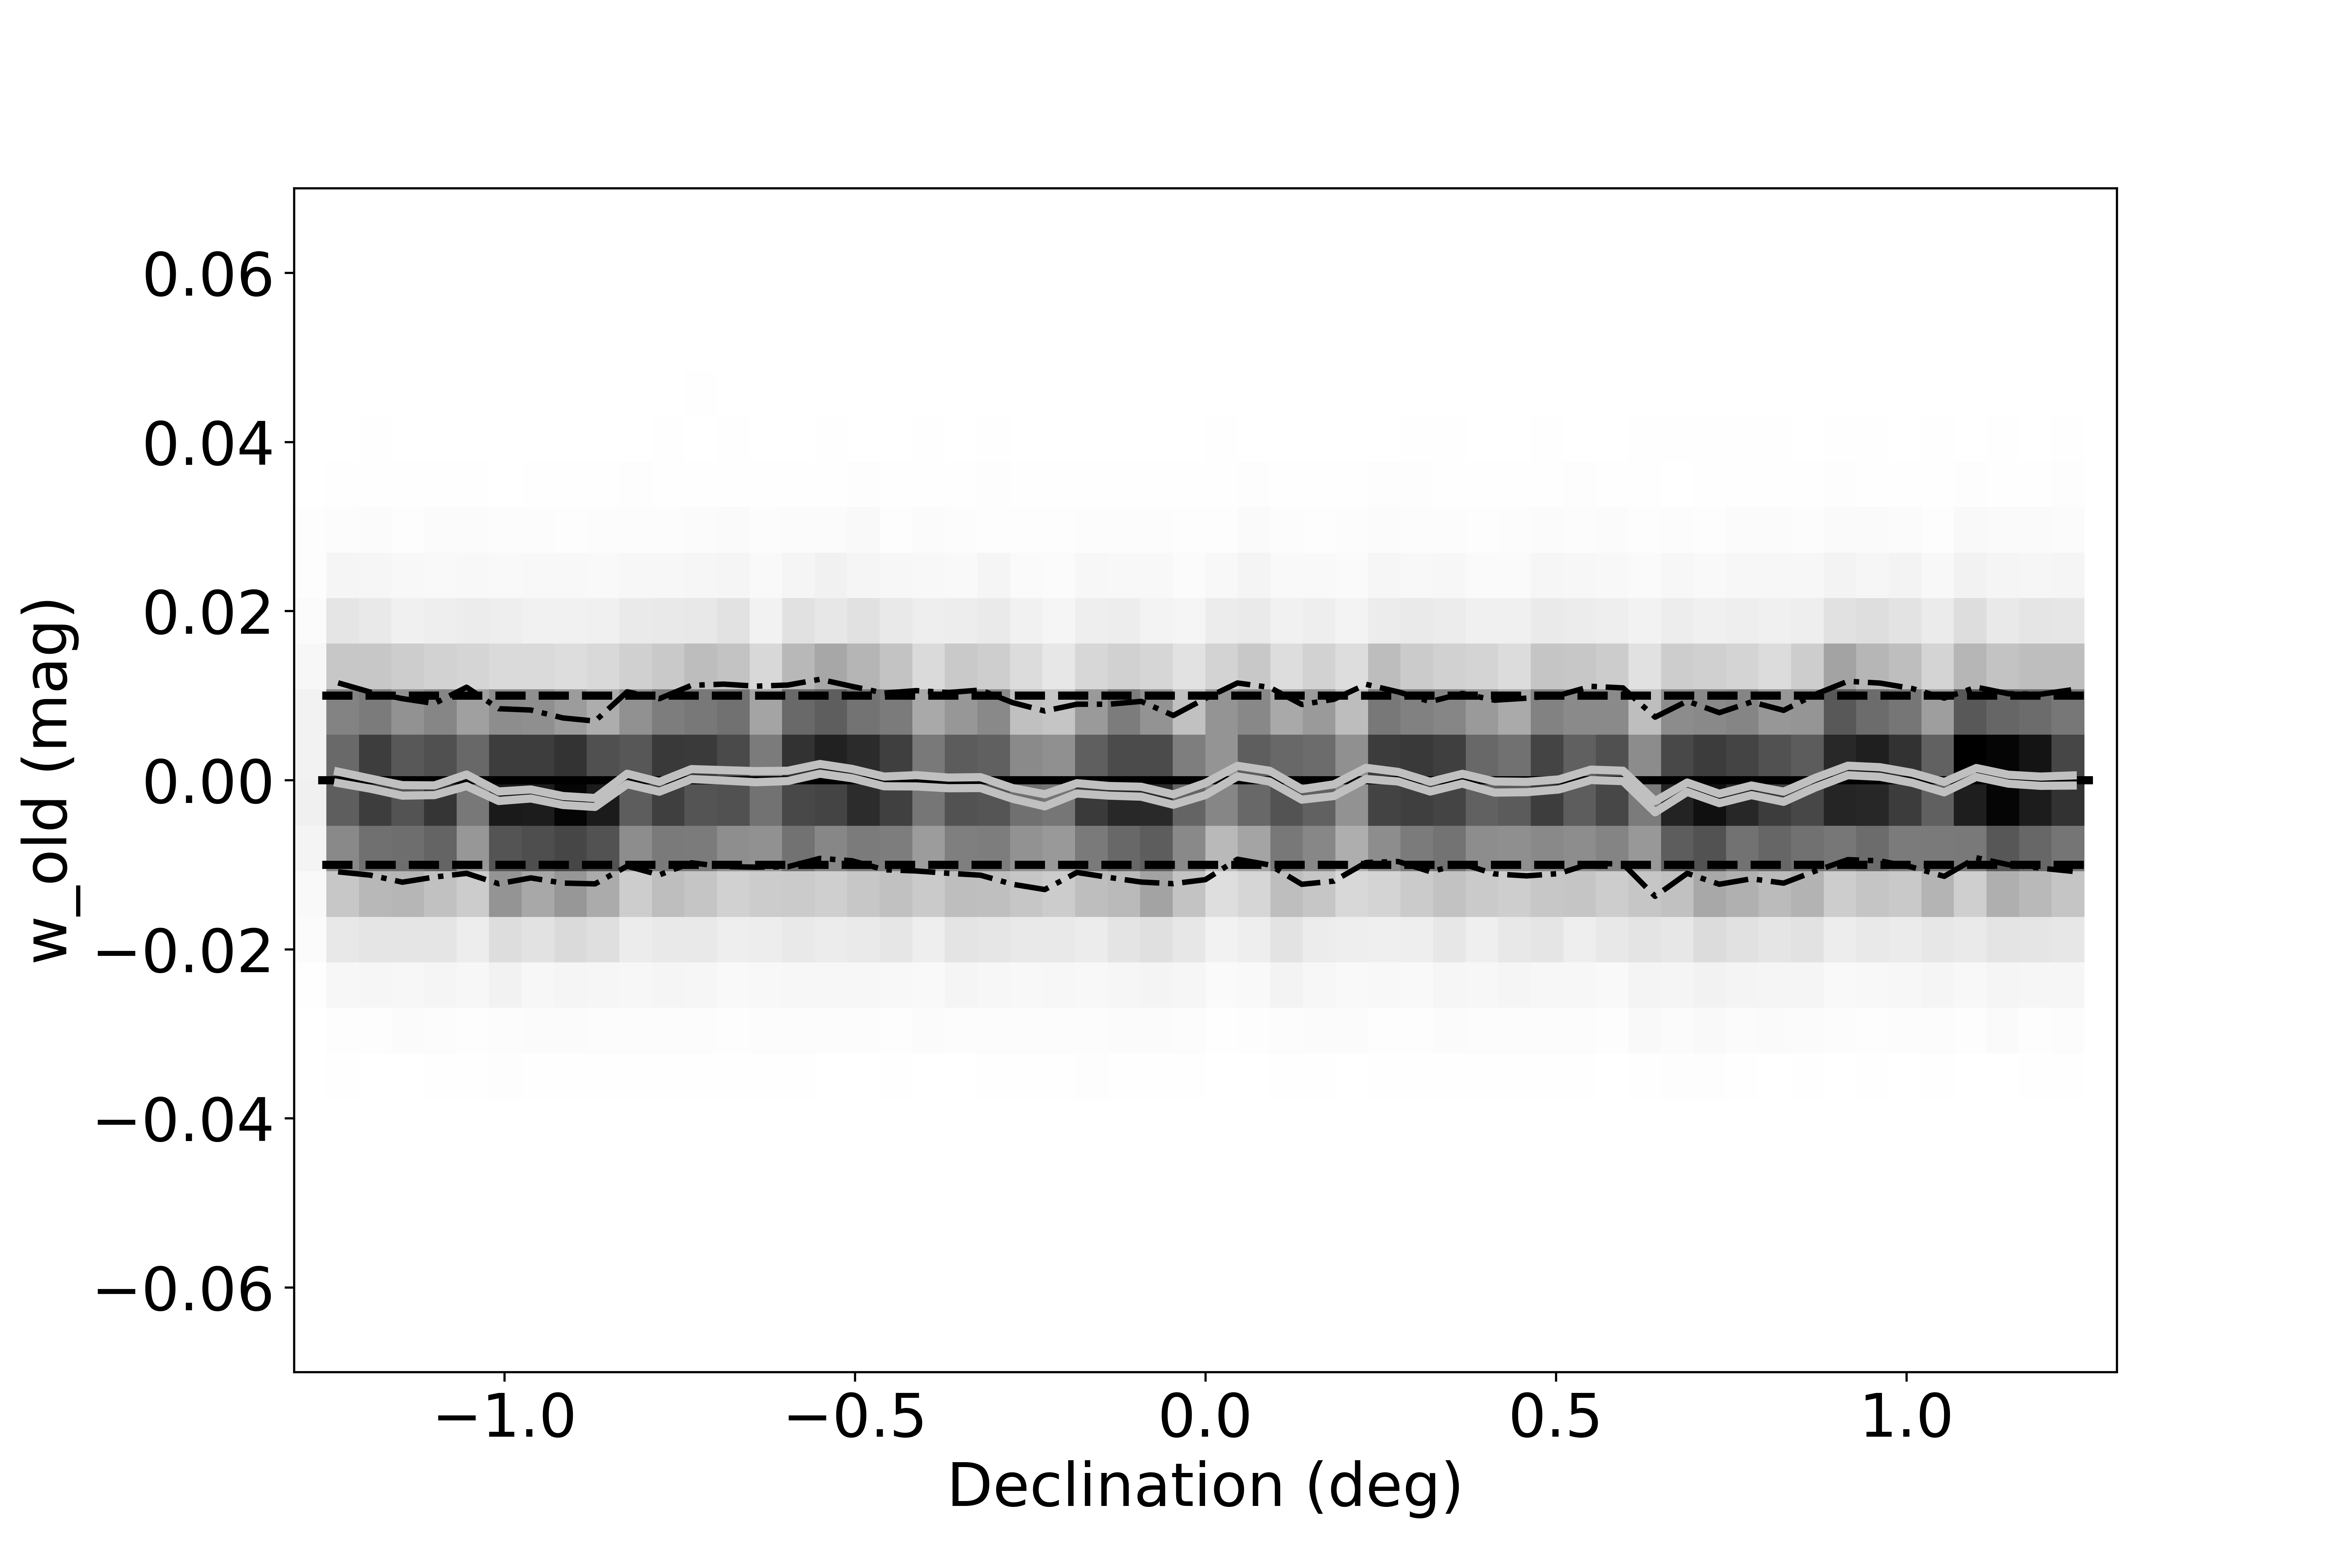
\includegraphics[width=7cm]{figures/testV26vsV33_r_w_old_Dec_Hess.png}
    \centering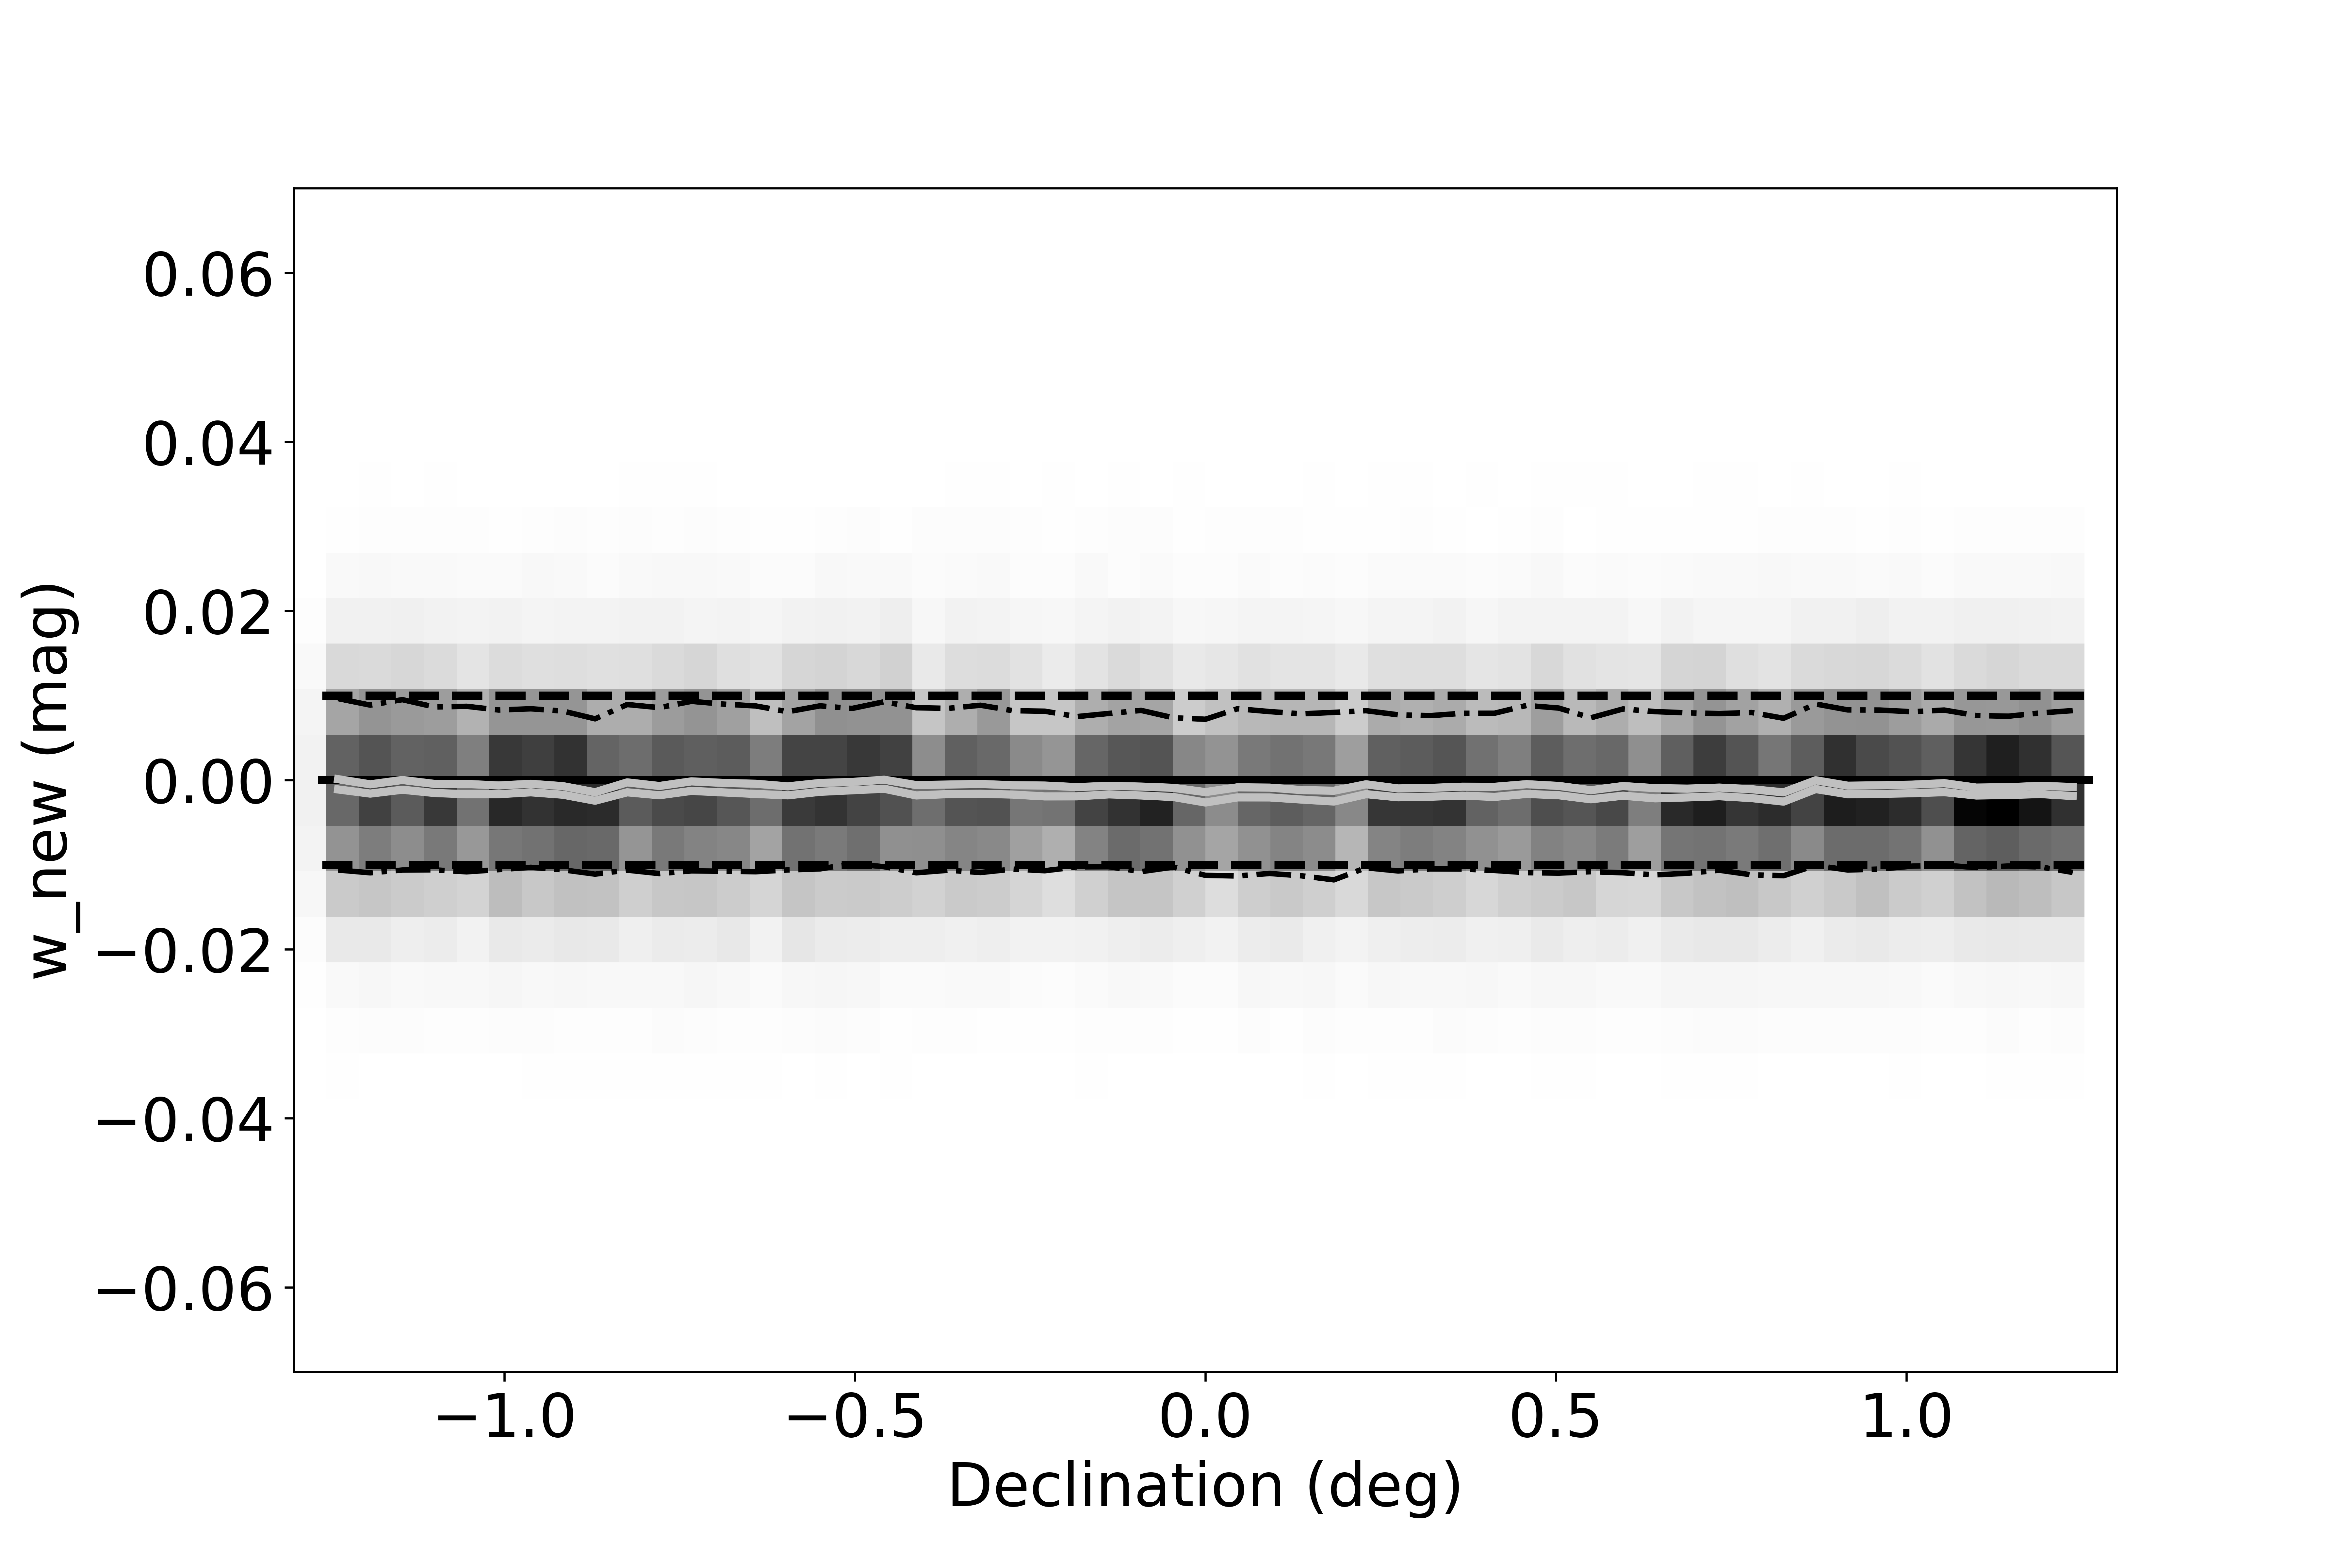
\includegraphics[width=7cm]{figures/testV26vsV33_r_w_new_Dec_Hess.png}
\caption{A comparison of the $w$ color, the second principal color in the SDSS
$r-i$ vs. $g-r$ color-color diagram, behavior for the v2.6 (left) and v3.4 (right)
catalogs. The standard deviation of the median $w$ values binned by R.A. and Dec
is 2.6 millimag and 1.1 millimag for v2.6 and 1.0 millimag and 0.3 millimag for v3.4,
respectively.}
\label{fig:comparew} 
\end{figure}
 

\begin{figure}[th!]
    \centering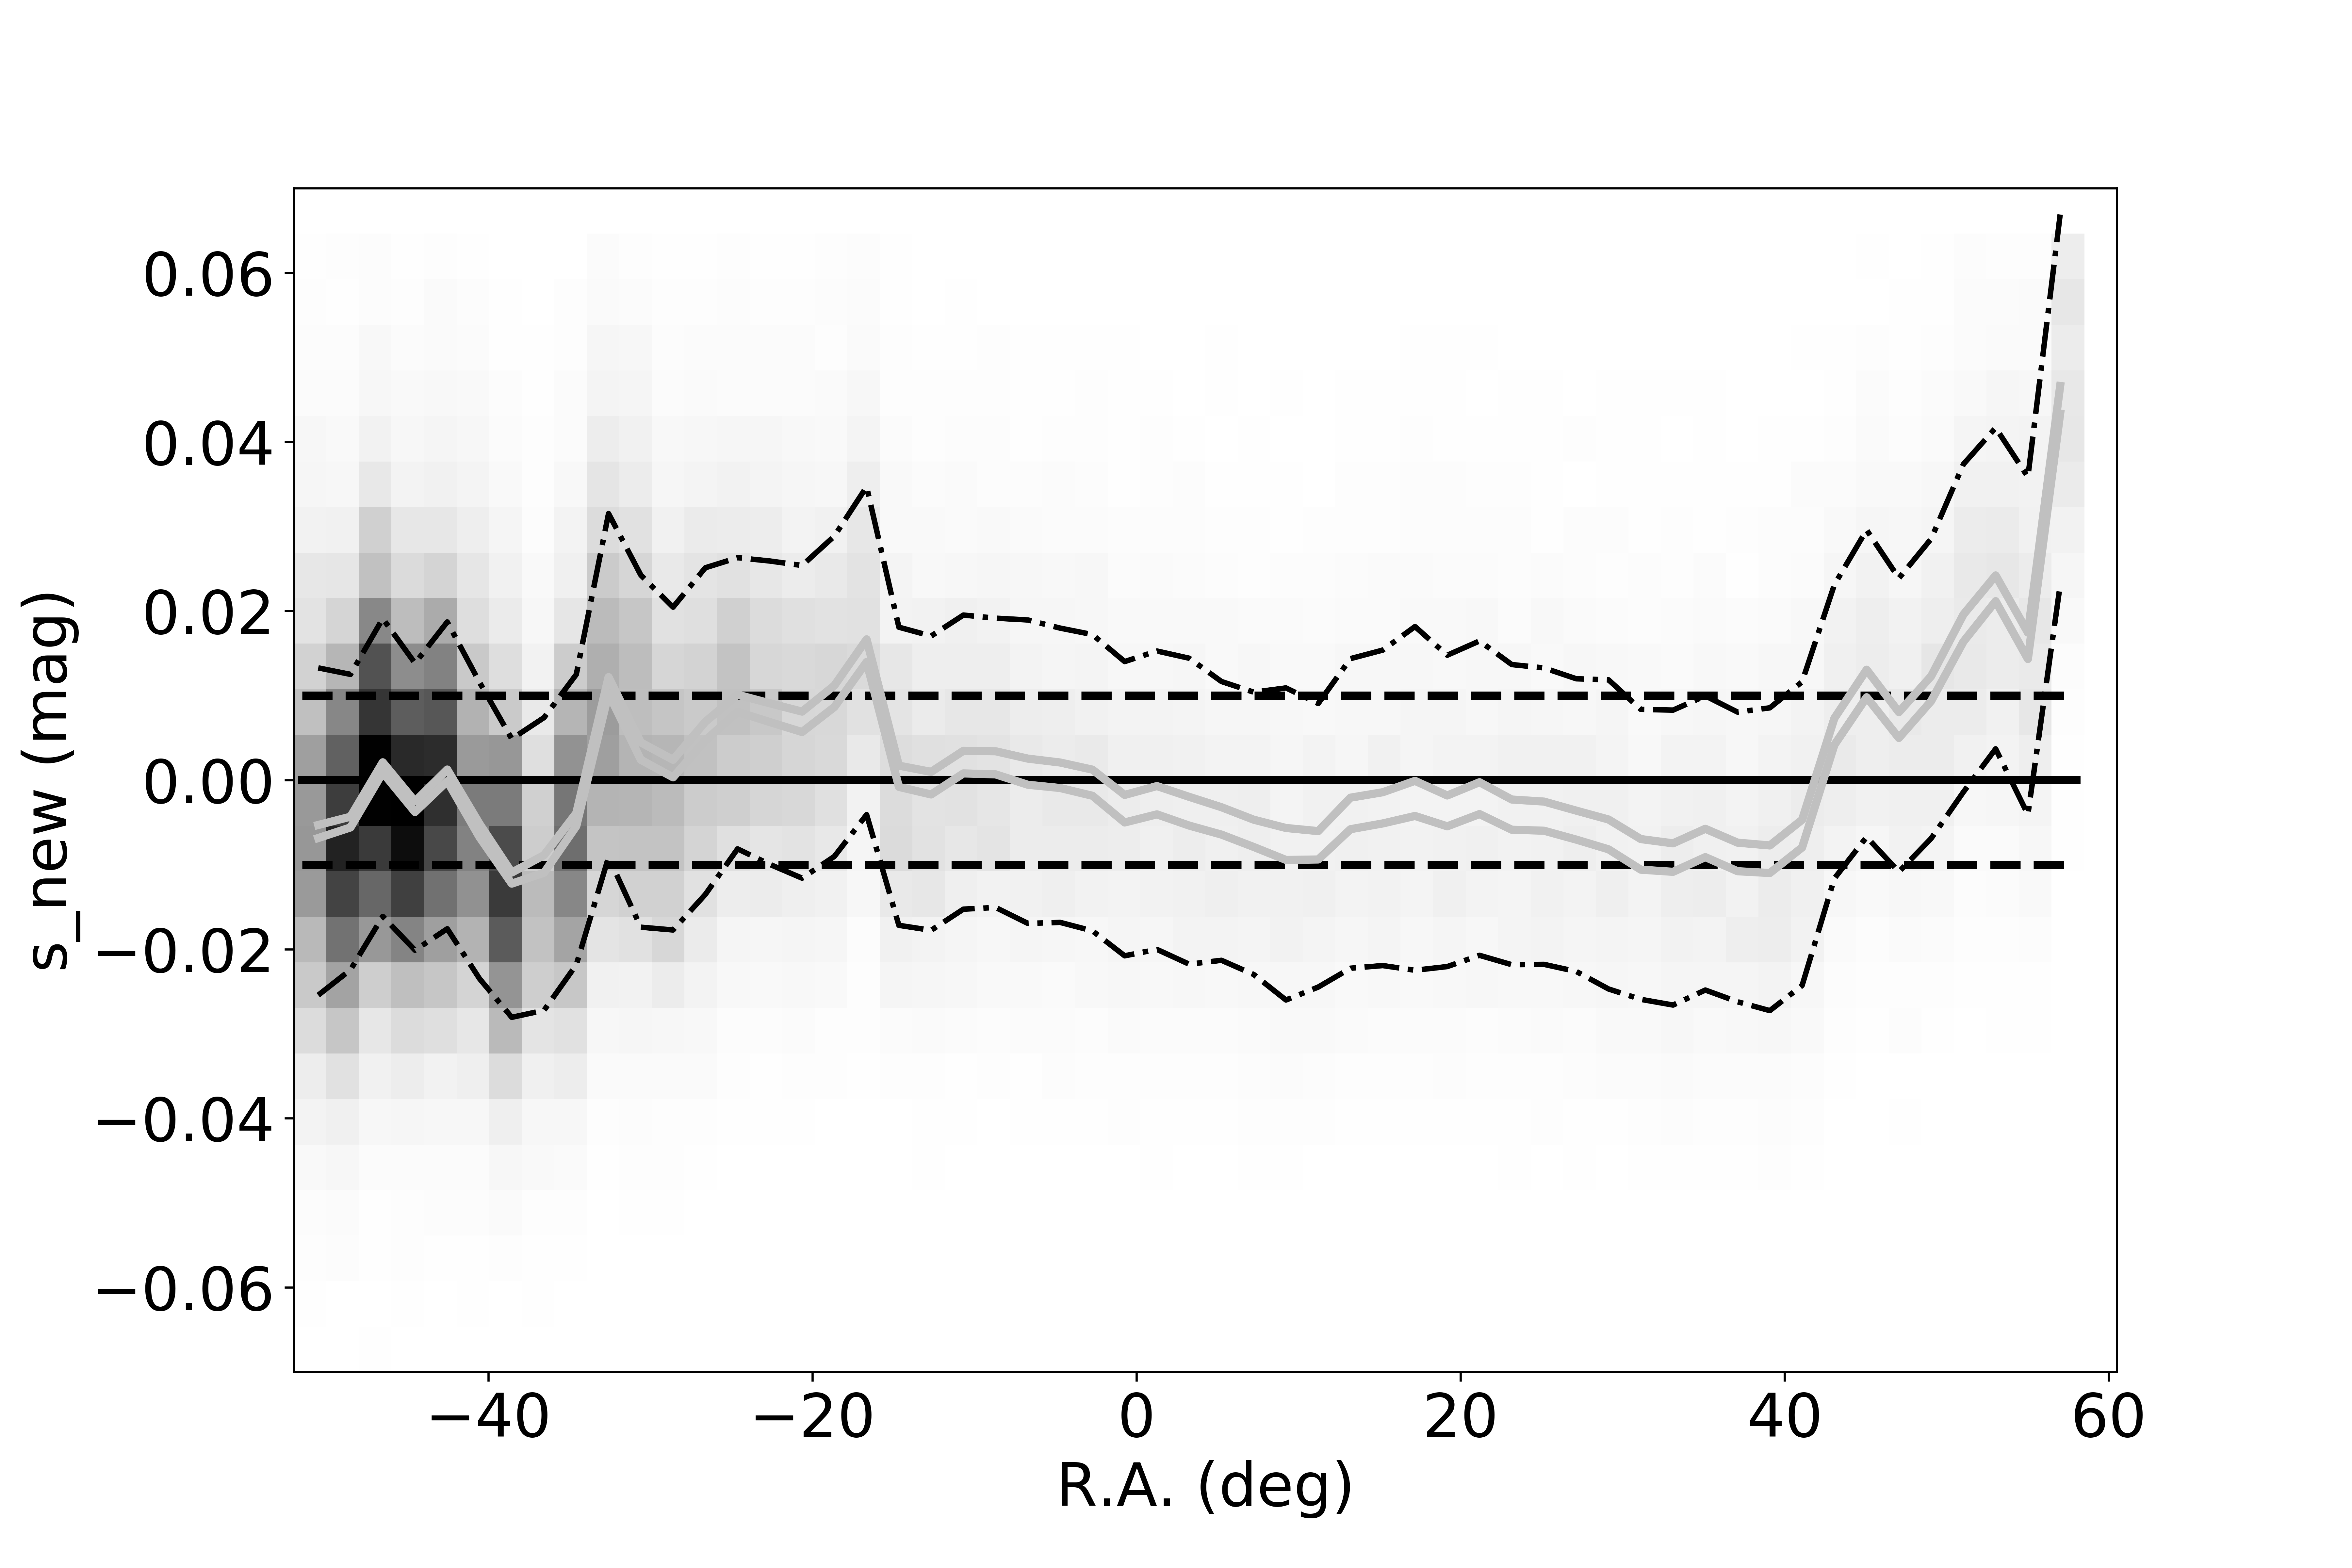
\includegraphics[width=7cm]{figures/testV26vsV33_snew_u_s_new_RA_Hess.png}
    \centering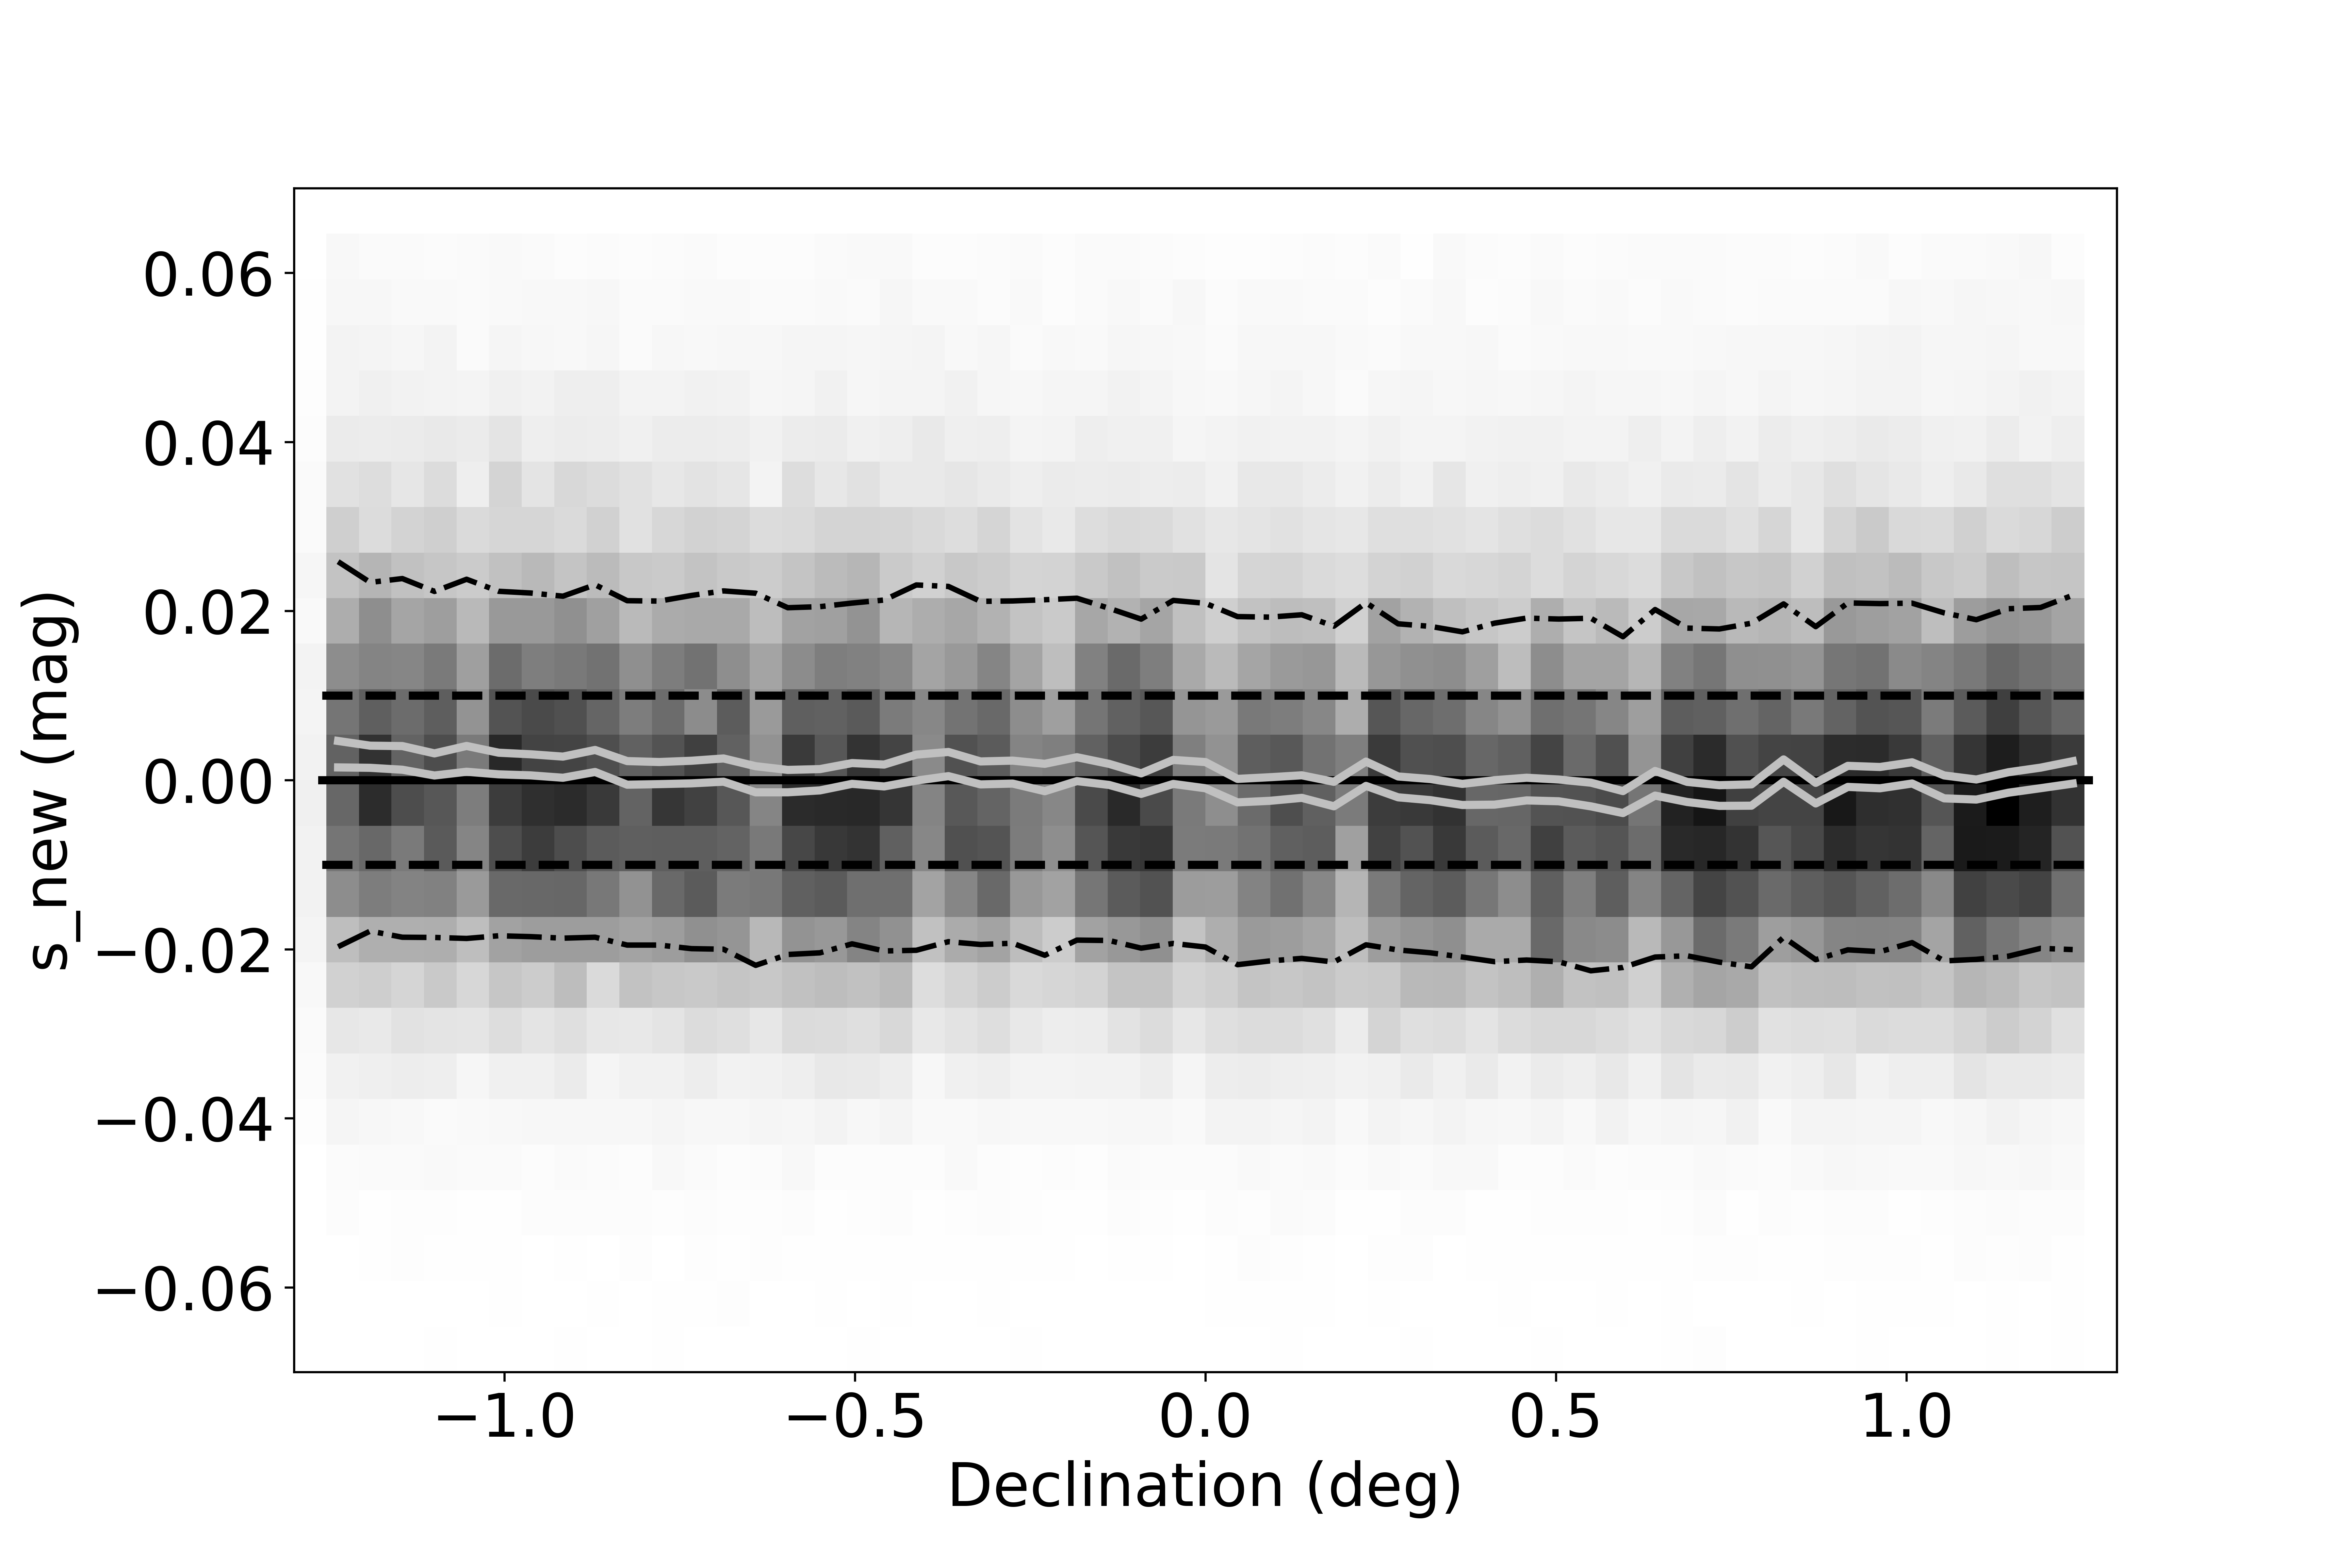
\includegraphics[width=7cm]{figures/testV26vsV33_snew_u_s_new_Dec_Hess.png} 
    \centering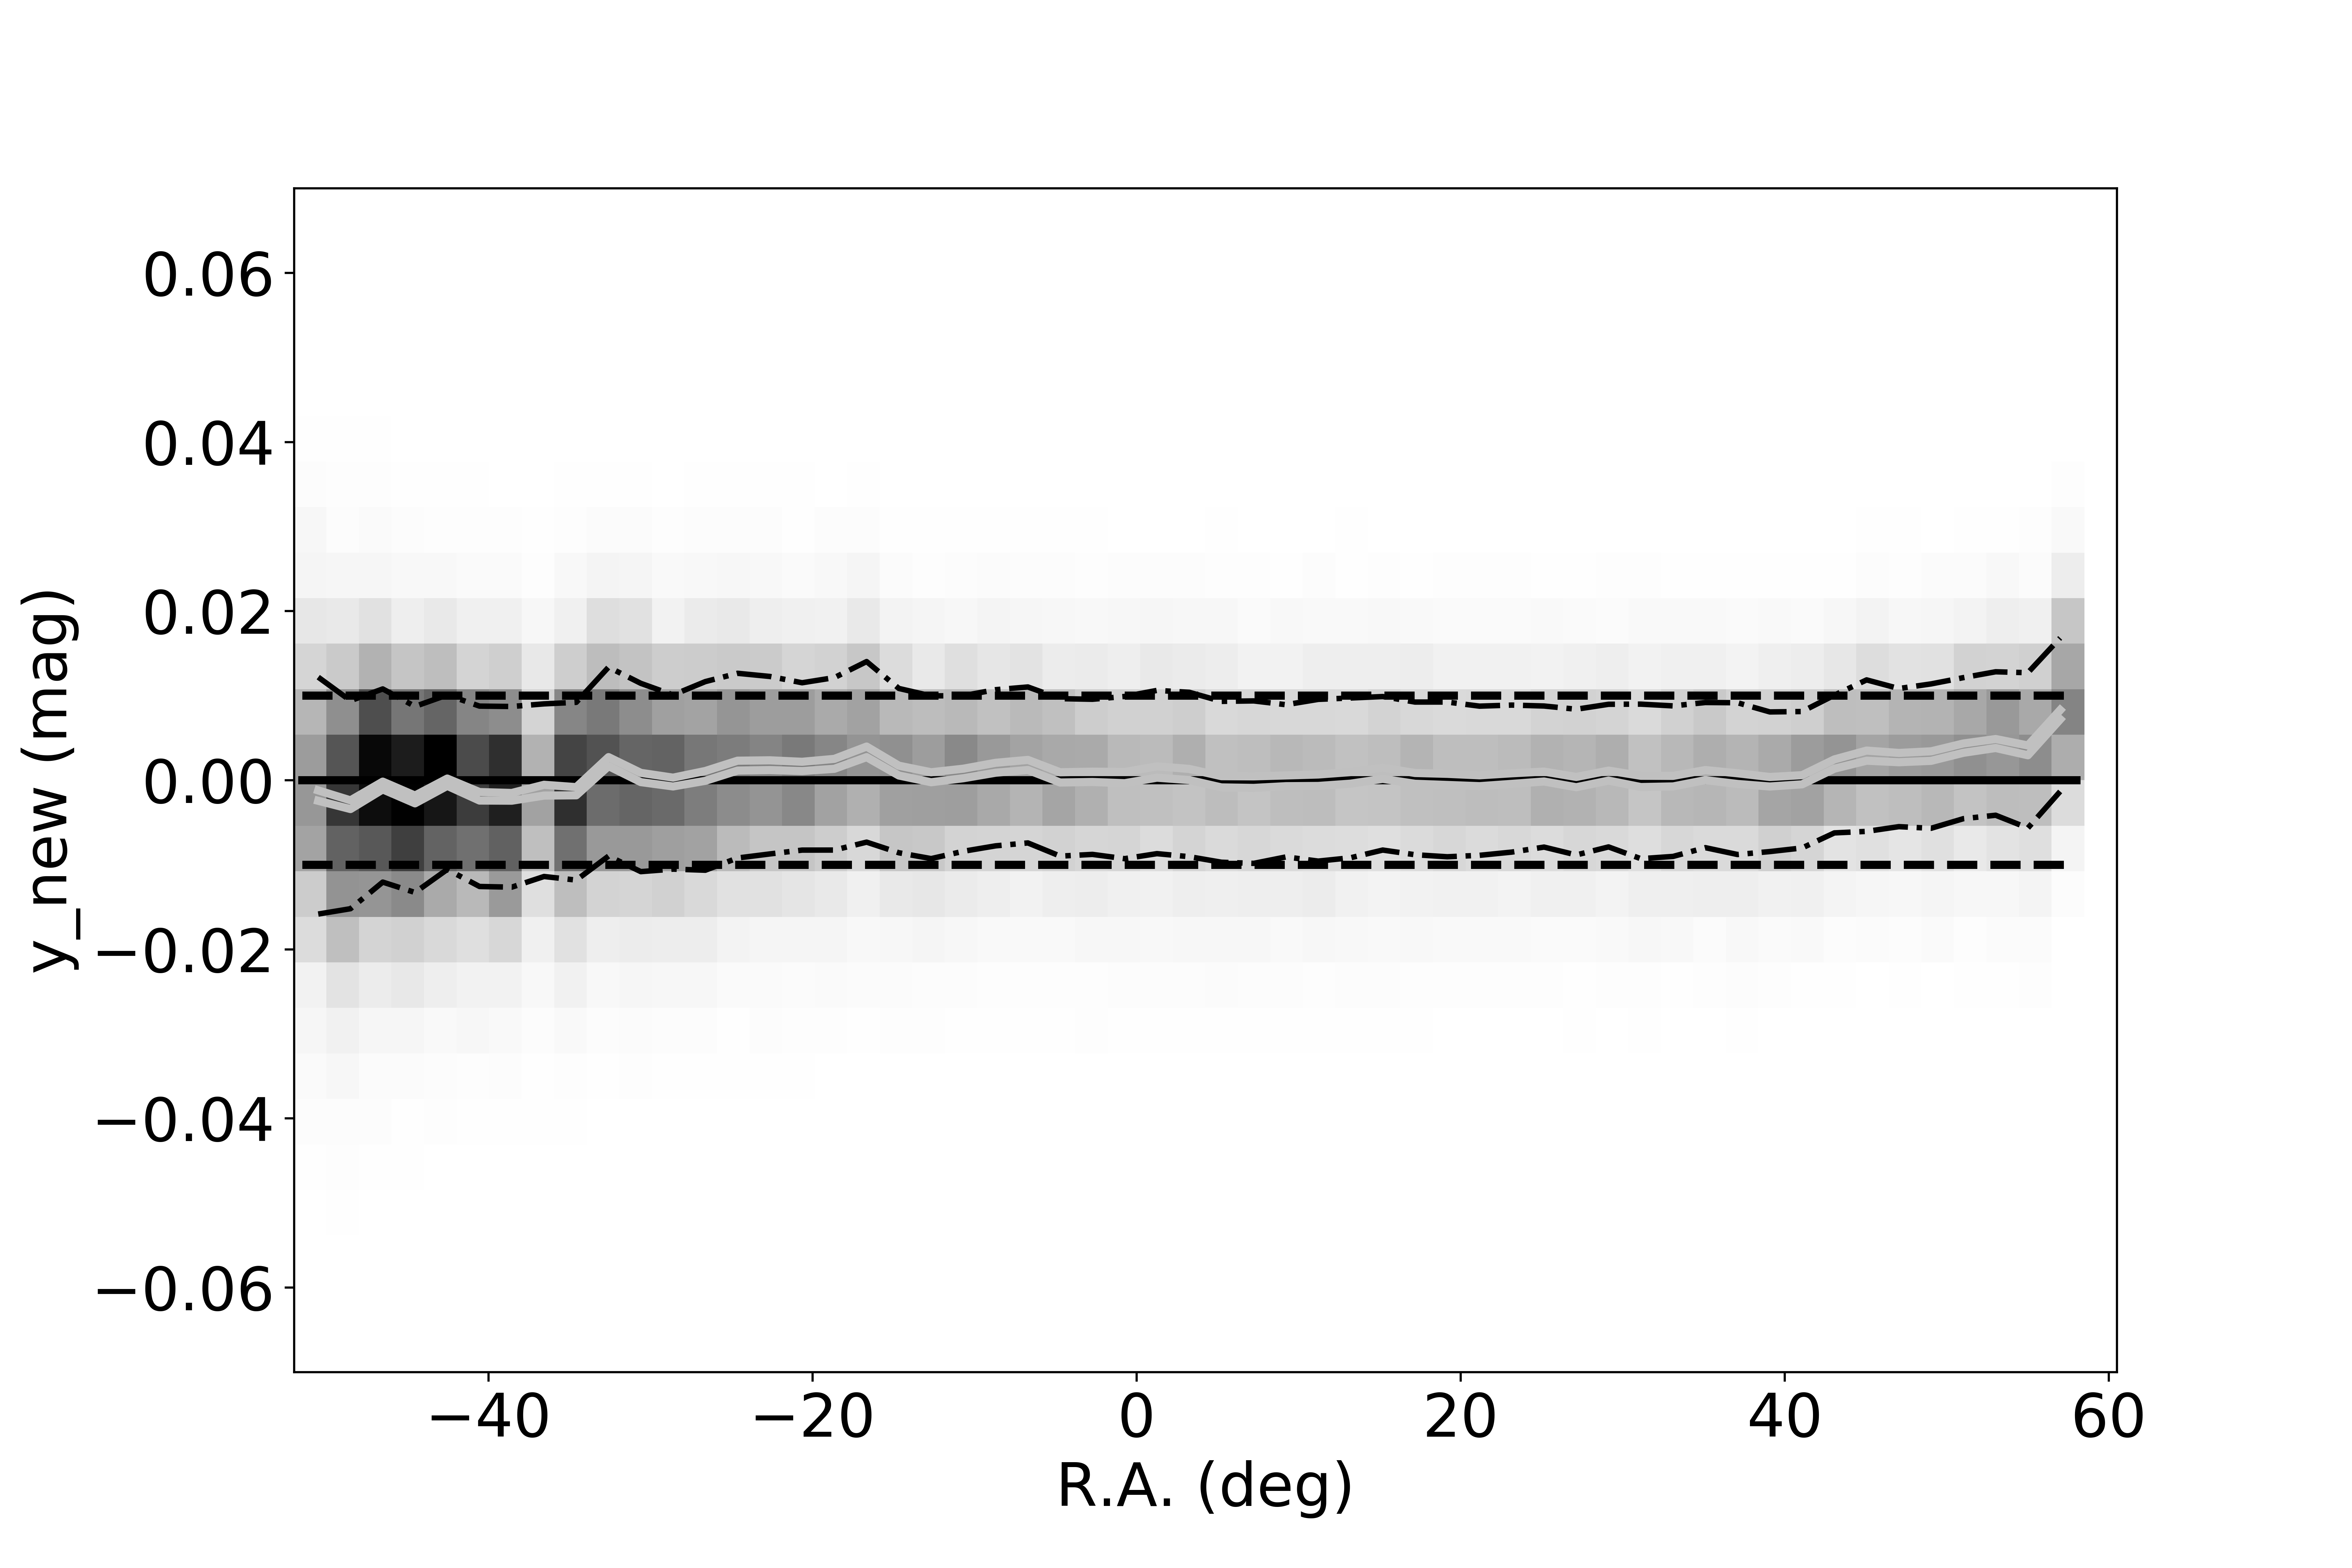
\includegraphics[width=7cm]{figures/testV26vsV33_ynew_z_y_new_RA_Hess.png} 
    \centering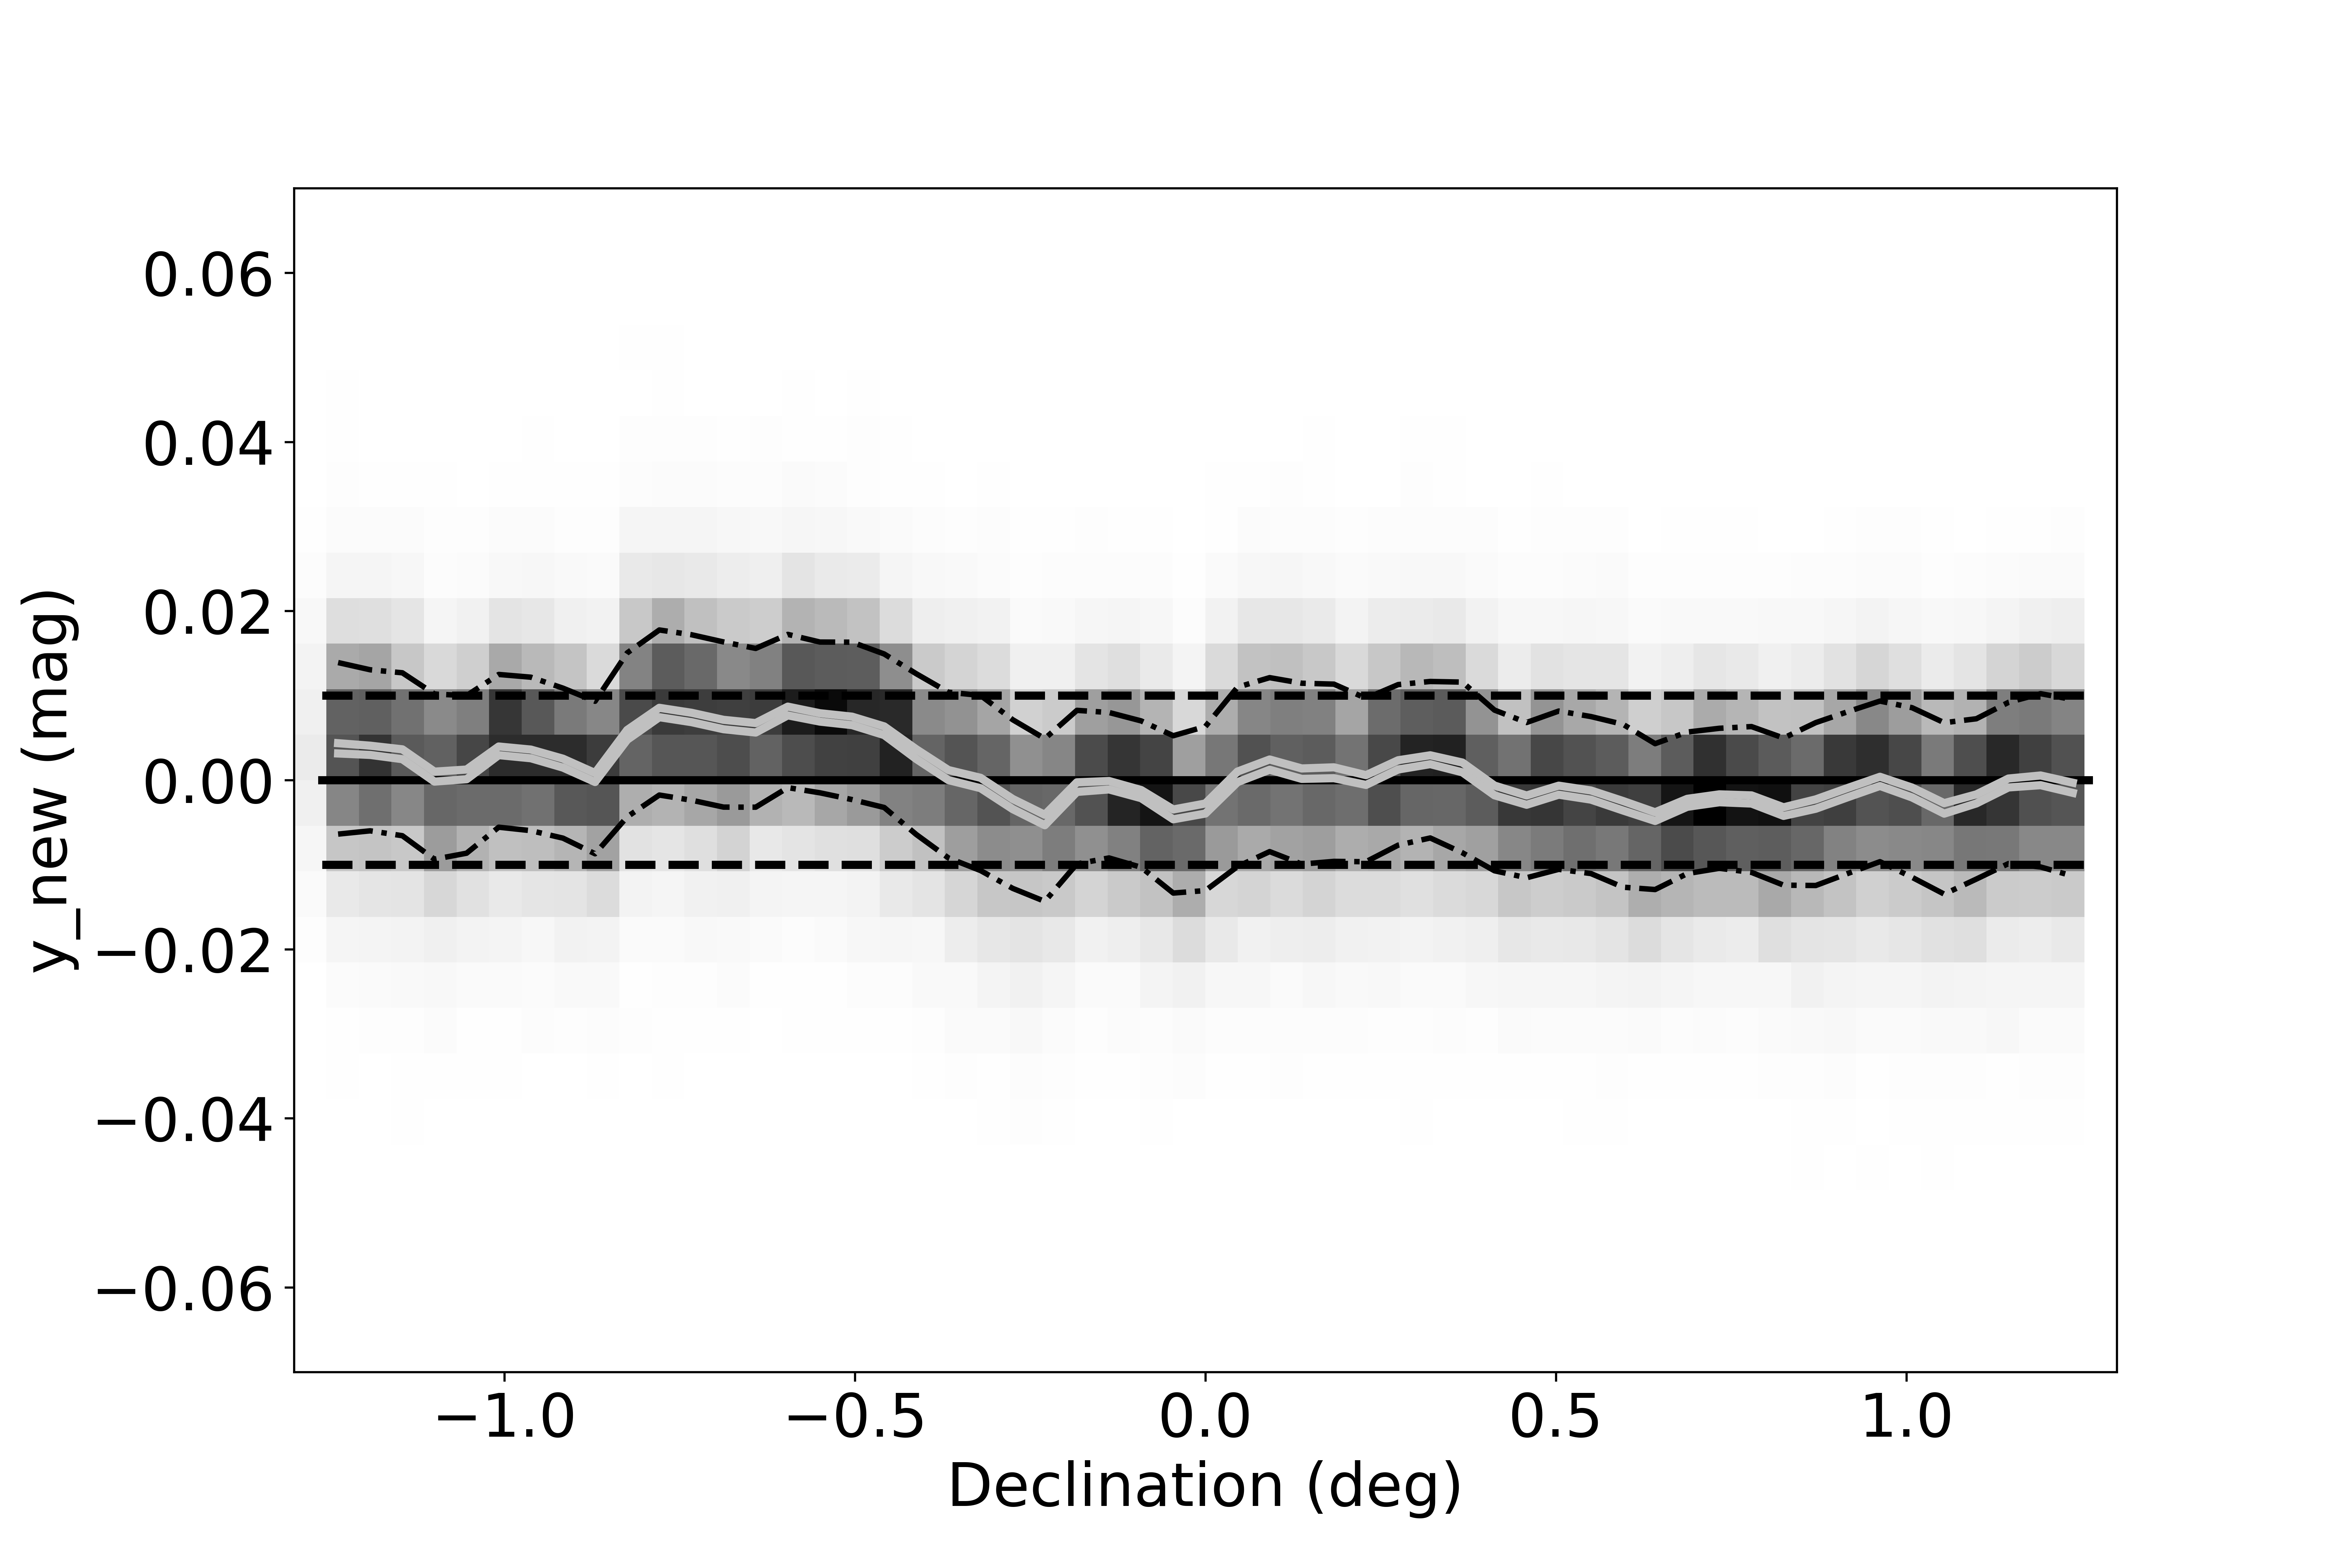
\includegraphics[width=7cm]{figures/testV26vsV33_ynew_z_y_new_Dec_Hess.png}  
\caption{The behavior of the $s$ color (top two panels), the second principal color in the SDSS
$g-r$ vs. $u-g$ color-color diagram, and the $y$ color (bottom two panels), the second 
principal color in the SDSS $i-z$ vs. $r-i$ color-color diagram, for the new v3.4 catalog.
The standard deviation of the median $s$ values binned by R.A. and Declination is 9.8 millimag 
and 1.3 millimag, respectively, and 1.8 millimag and 3.4 millimag for the $y$ color.}
\label{fig:comparesy} 
\end{figure}
  

\subsection{Comparison of the new v3.4 SDSS catalog with DES and Pan-STARRS catalogs \label{sec:DESPS1}} 
  
The quality of photometric zeropoint calibration for the new SDSS catalog can be conveniently
tested with the DES (see Section~\ref{ssec:des}) and Pan-STARRS (see Section~\ref{ssec:ps1}) catalogs. 
Both catalogs list $griz$ photometry of sufficient precision for esentially all stars
from Stripe 82. Their photometric calibration procedures are expected to result in different 
spatial patterns and thus a cross-comparison with the v3.4 catalog can reveal residual problems
with zeropoint calibration. They are also deeper than Gaia DR2 catalog and thus can provide
further clues about the Gmag discrepancy at Gaia's faint end illustrated in Figure~\ref{fig:gaiaJump}. 

Our comparison of the magnitude differences is illustrated in Figures~\ref{fig:DESPSRA} and \ref{fig:DESPSDec},
and the robust standard deviation for binned median magnitude differences is listed in Table~\ref{tab:DESPS1}. 
This multi-survey comparison indicates that the spatial variation of photometric zero points in the 
updated SDSS catalog is well below 0.01 mag (rms), with typical values of 3-7 millimag in the R.A. 
direction and 1-2 millimag in the Declination direction. As discernible in the two bottom panels
in Figure~\ref{fig:DESPSRA}, there are systematic residual errors in the $z$ band zeropoint as a 
function of  Declination at the level of a few millimag. Note also implied DES $z$ band zeropoint errors 
of up to 0.01-0.02 mag, as a function of R.A. (see the bottom left panel in Figure~\ref{fig:DESPSRA}). 

The variation of the magnitude differences
with magnitude (see Figure~\ref{fig:drVSr}) shows good agreement (to within $\sim$5 millimag) 
even at the faint end ($20<r<21$), where Gaia Gmag magnitudes appear too faint by about
0.02 mag, and thus demonstrates a likely problem with Gaia DR2 photometry. 
 
\begin{deluxetable}{l|c|c|c|c}[ht!]
\tablecaption{The robust standard deviation for binned median magnitude differences between
the new v3.4 SDSS catalog, and DES and Pan-STARRS1 (PS1) catalogs (millimag). \label{tab:DESPS1}}
\tablehead{
\colhead{Band} & \colhead{DES R.A.} & \colhead{DES Dec} & \colhead{PS1 R.A.} & \colhead{PS1 Dec} 
}
\startdata
       $g$        &        5.1    &      1.8   &        3.4    &      1.4        \\
       $r$         &        4.1    &      0.8   &        2.6    &      0.7         \\  
       $i$         &        7.3    &      1.6   &        3.2    &      1.0         \\ 
       $z$        &       13.6    &     3.6   &        6.8    &      2.3         \\ 
\enddata
\end{deluxetable}
   

\begin{figure}[th!]
    \centering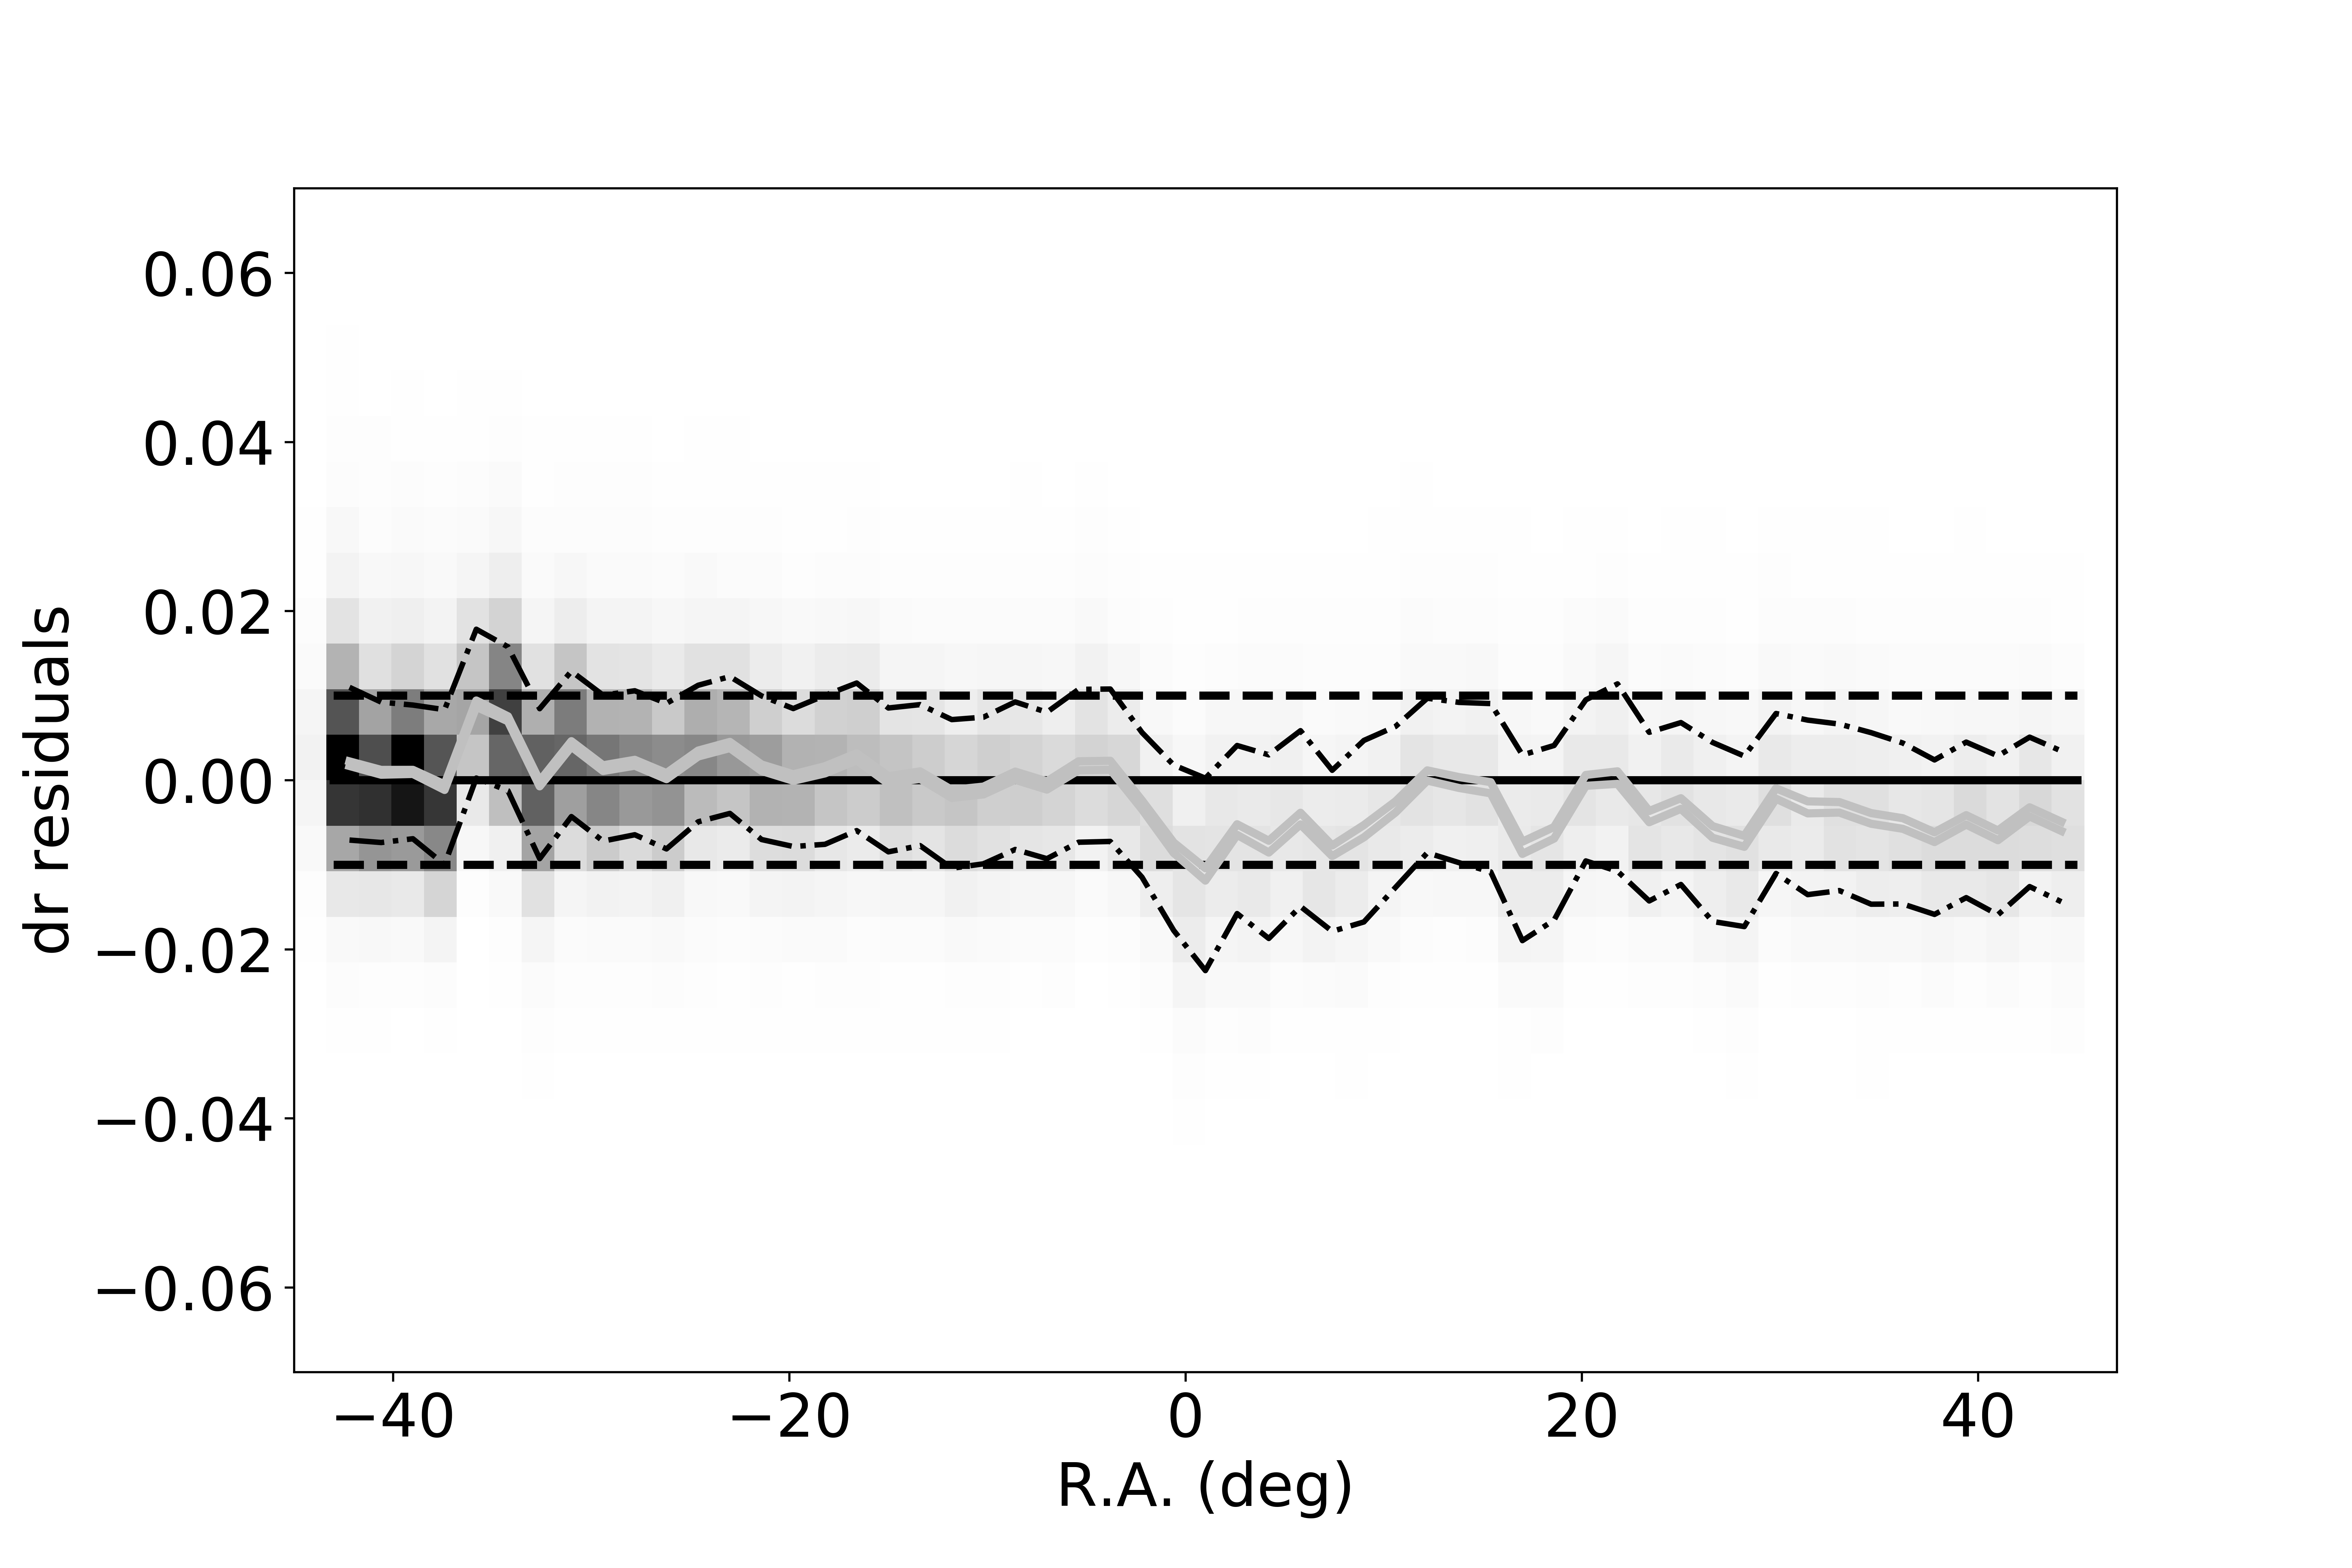
\includegraphics[width=7cm]{figures/colorResidDES2bright_dr_RA_Hess.png}
    \centering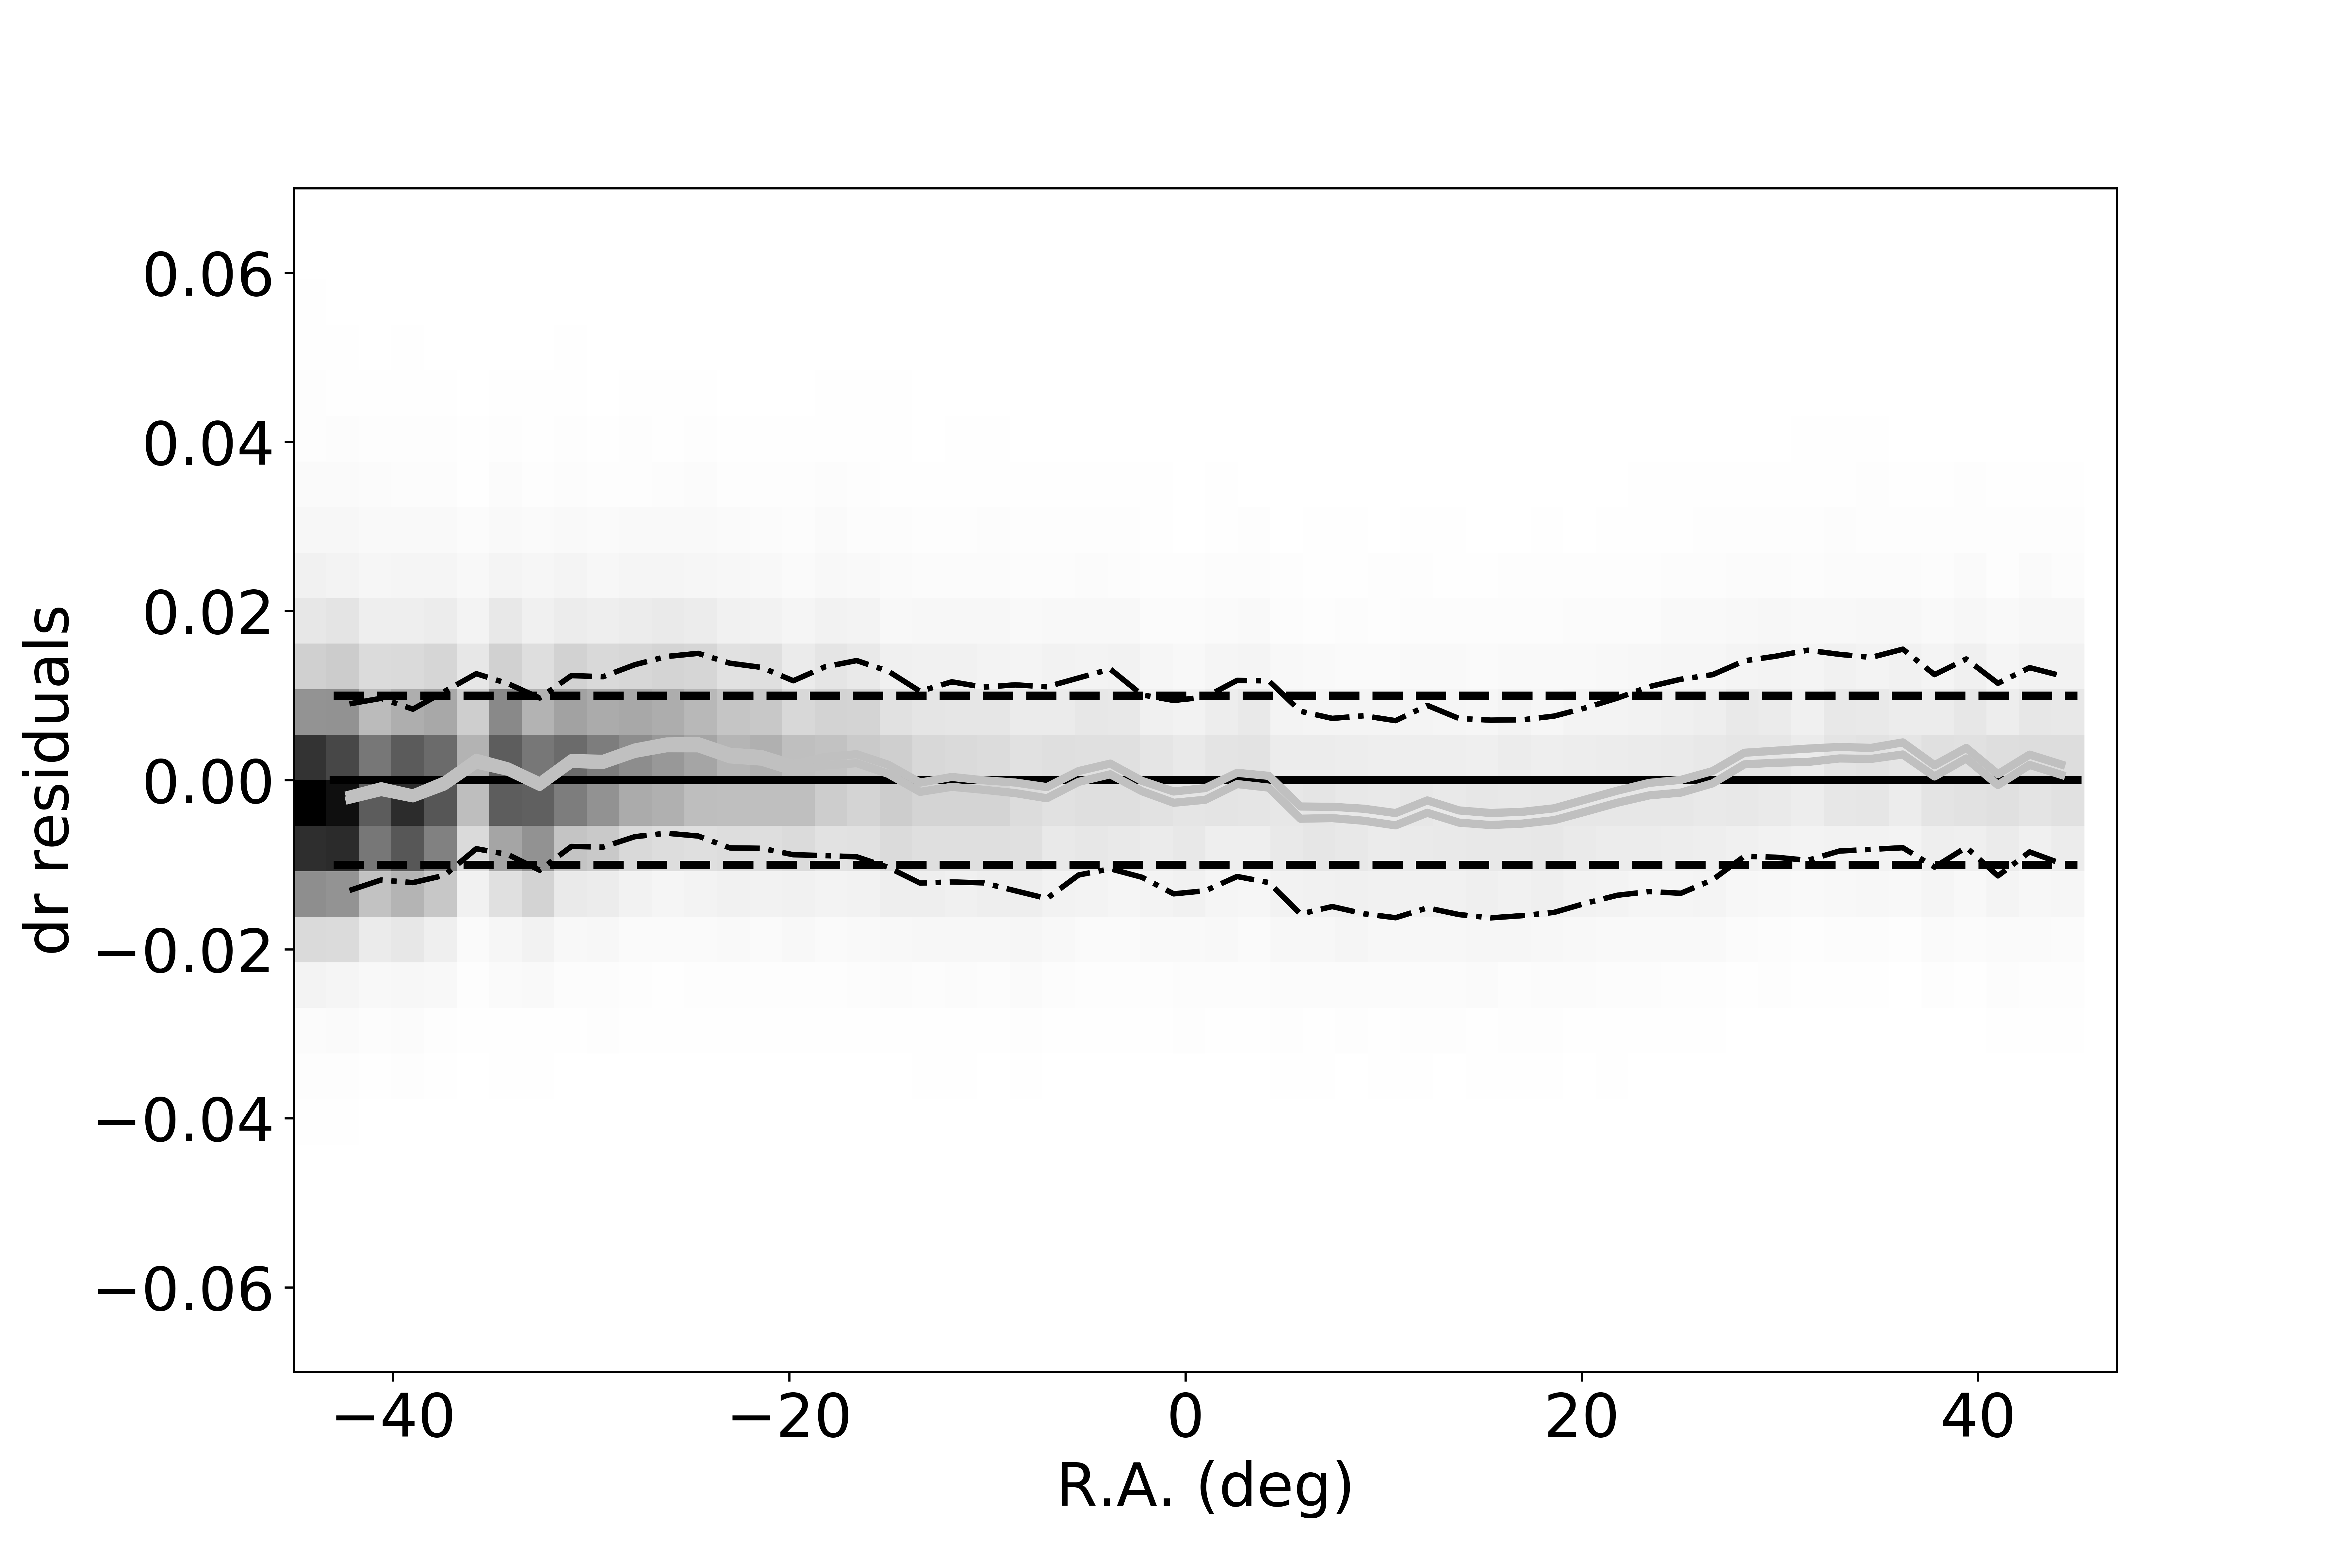
\includegraphics[width=7cm]{figures/colorResidPSbright_dr_RA_Hess.png}
    \centering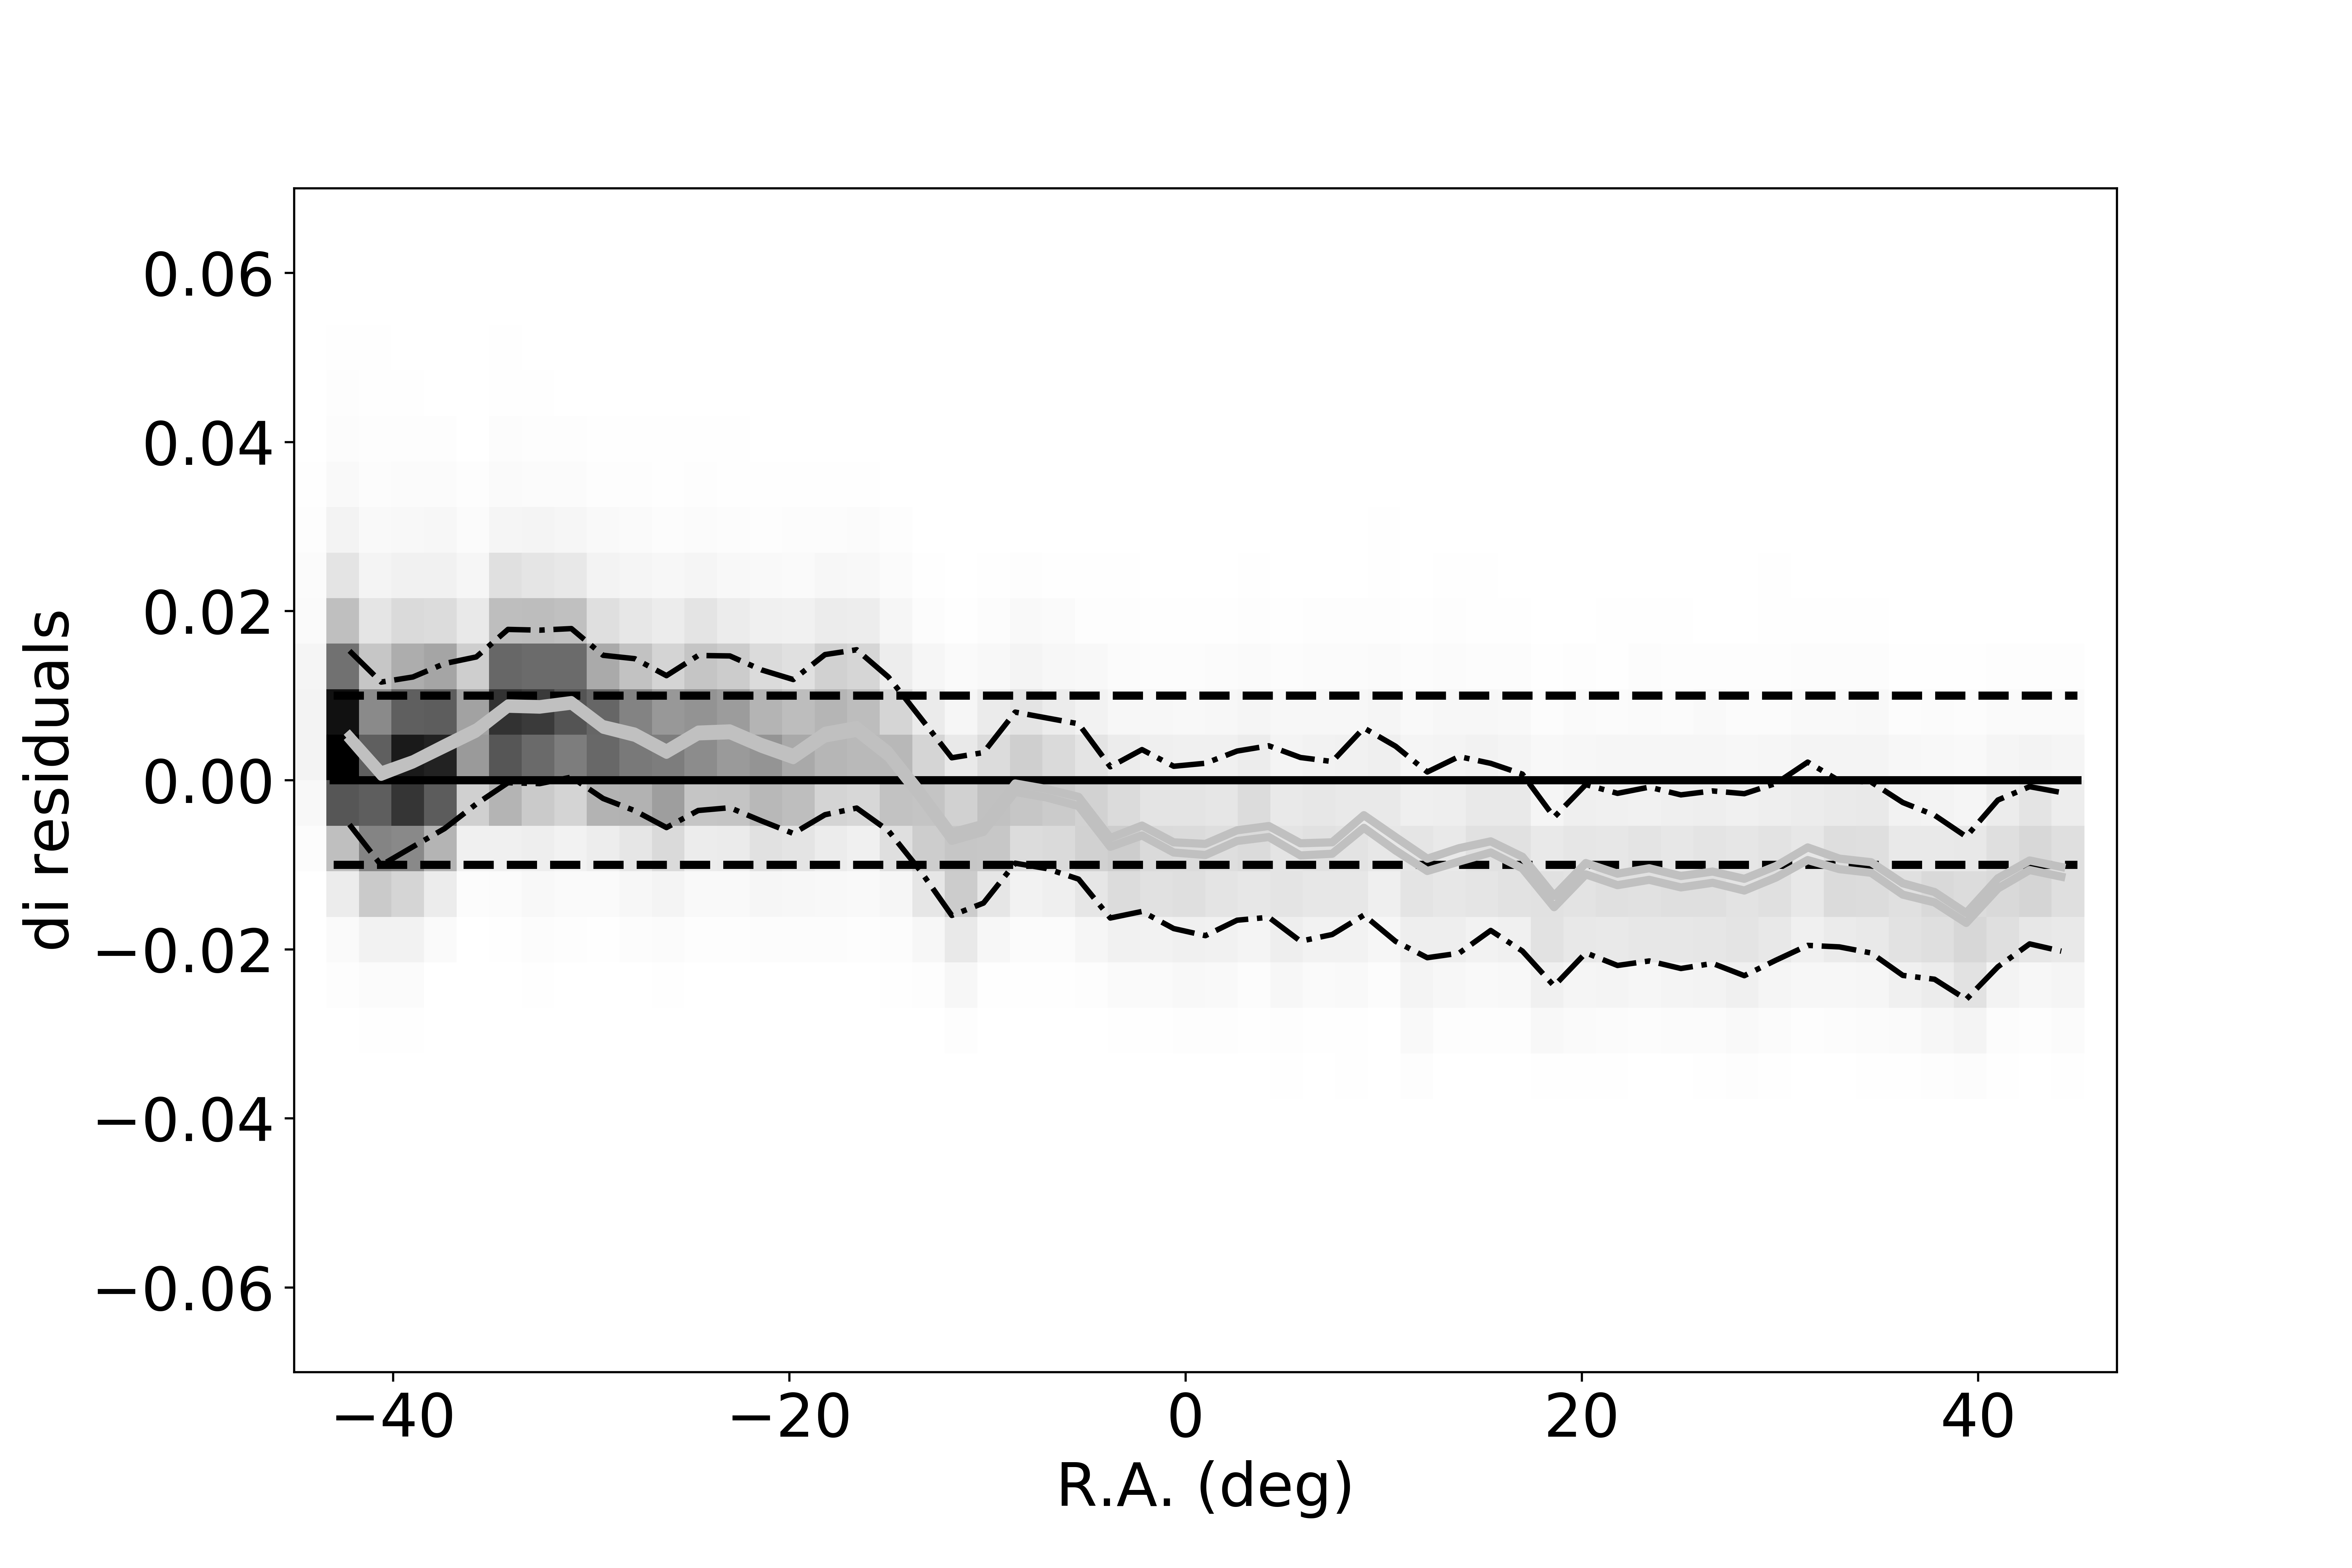
\includegraphics[width=7cm]{figures/colorResidDES2bright_di_RA_Hess.png}
    \centering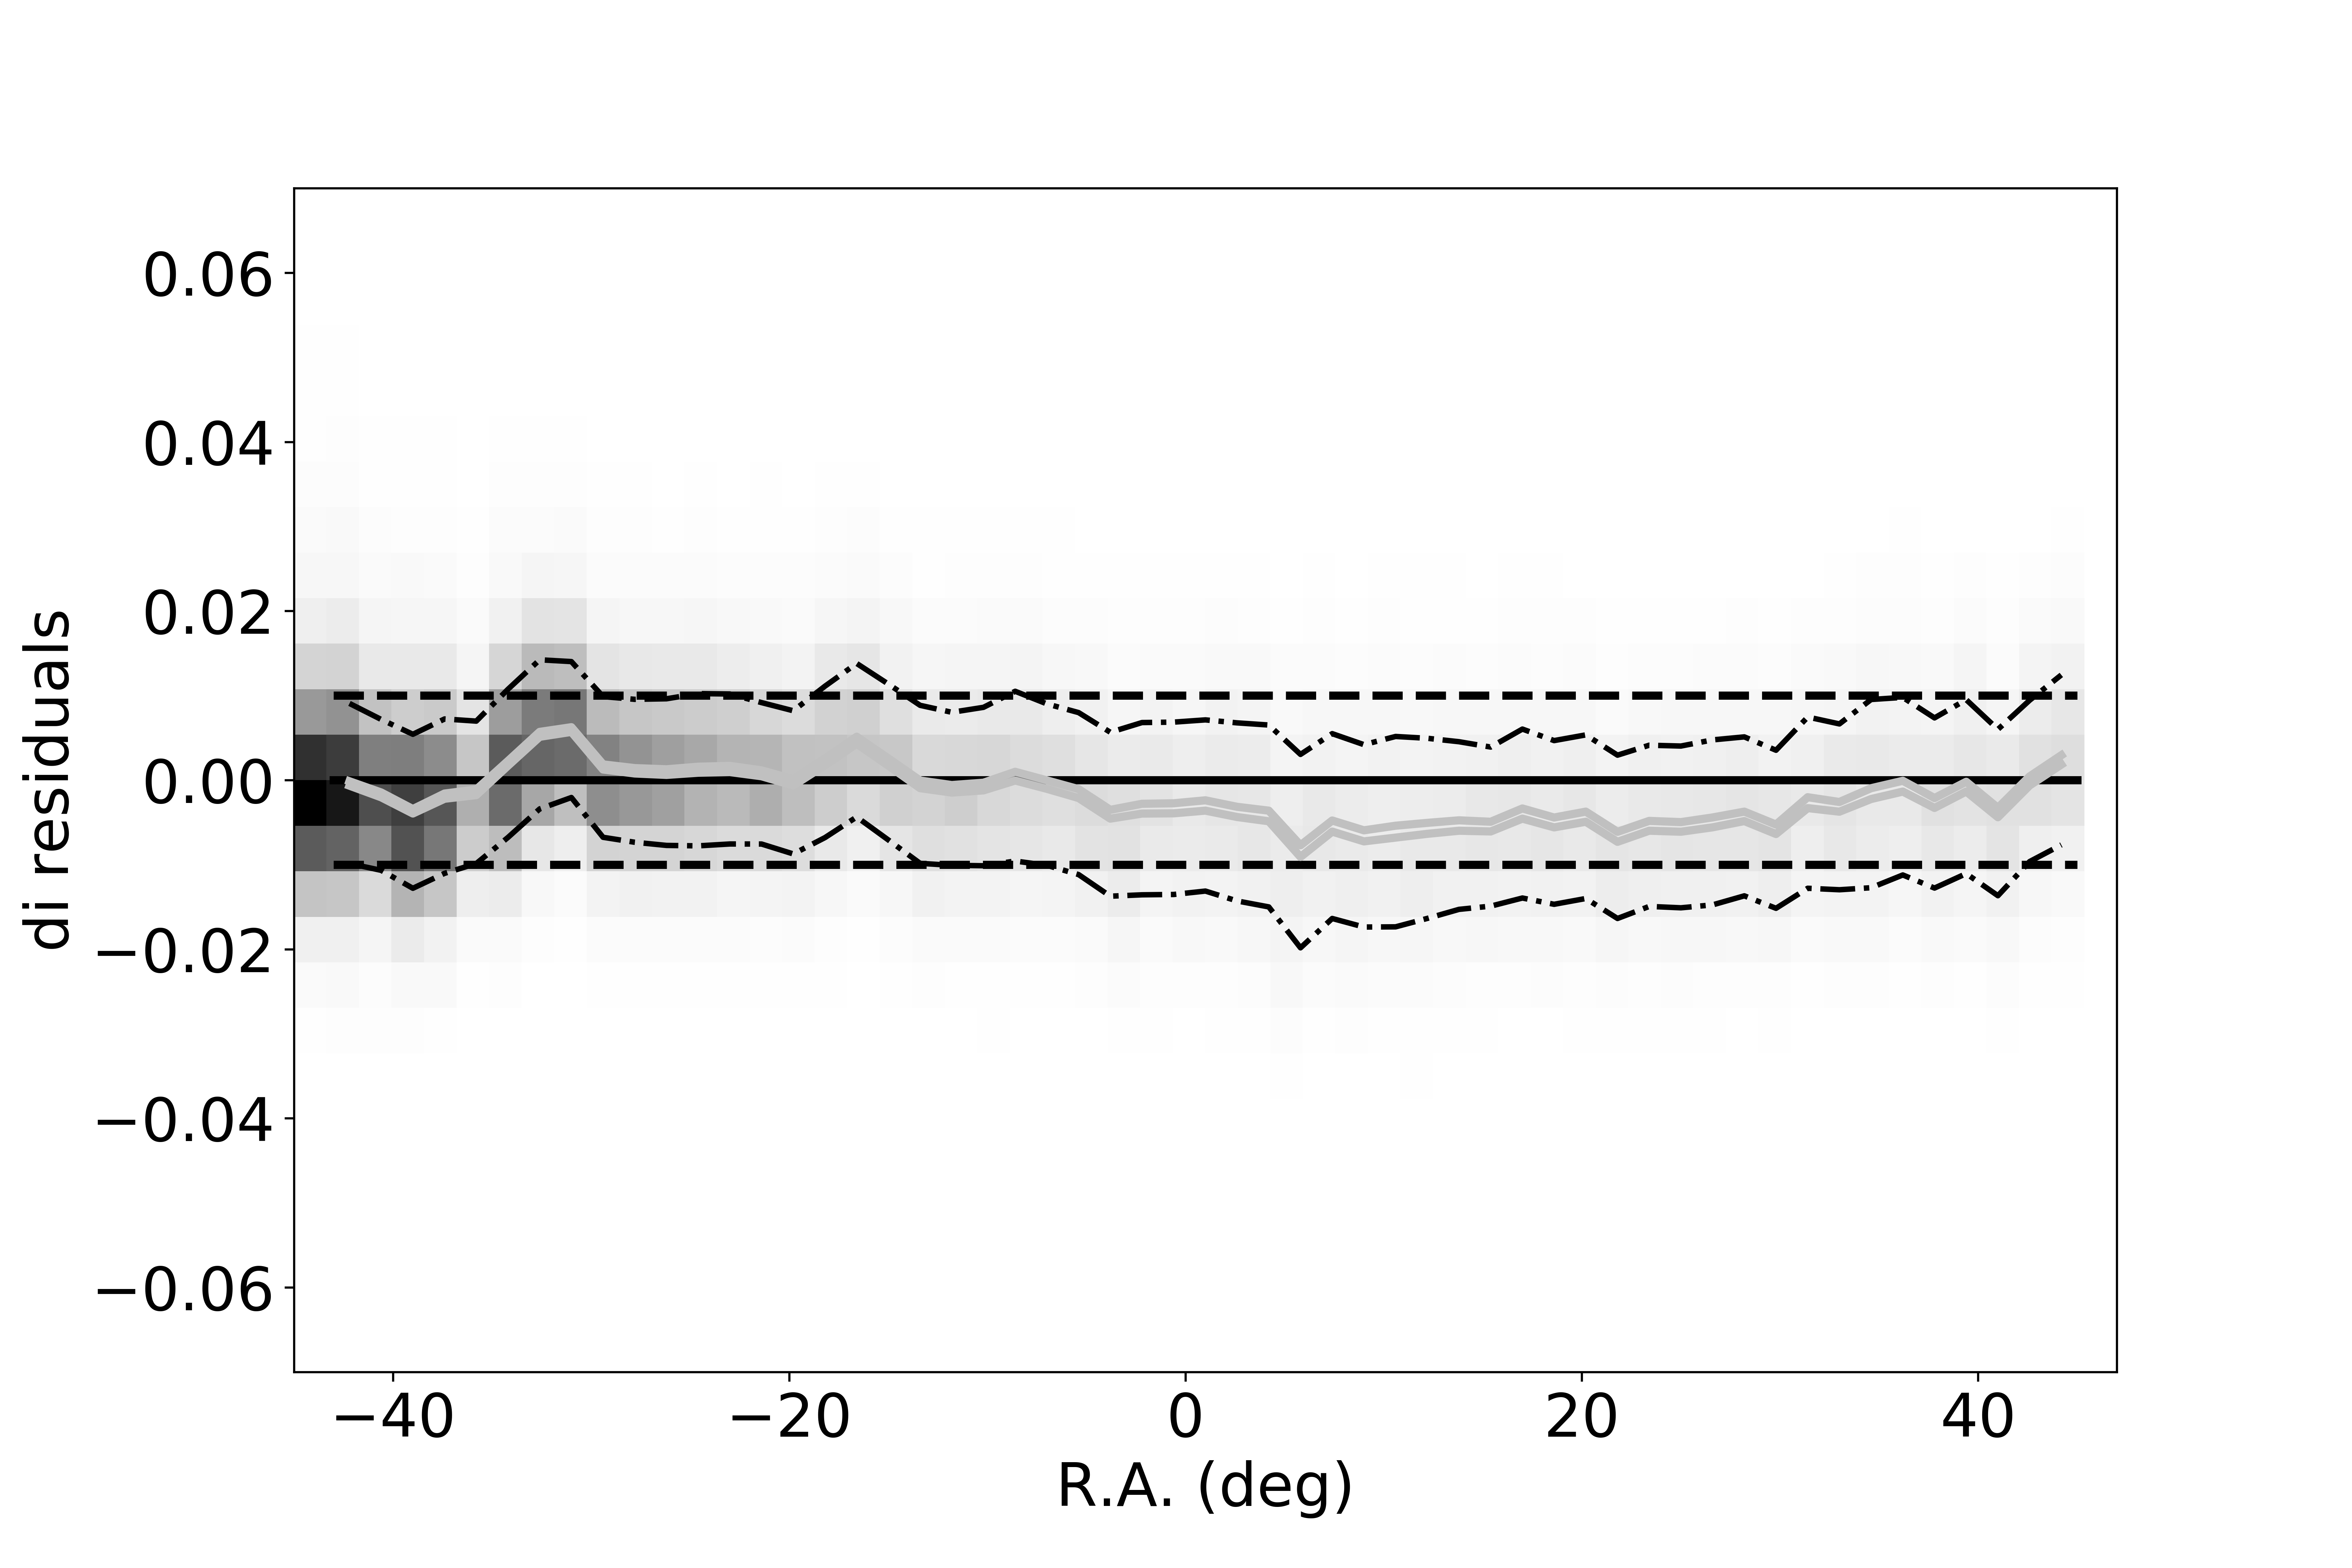
\includegraphics[width=7cm]{figures/colorResidPSbright_di_RA_Hess.png}
    \centering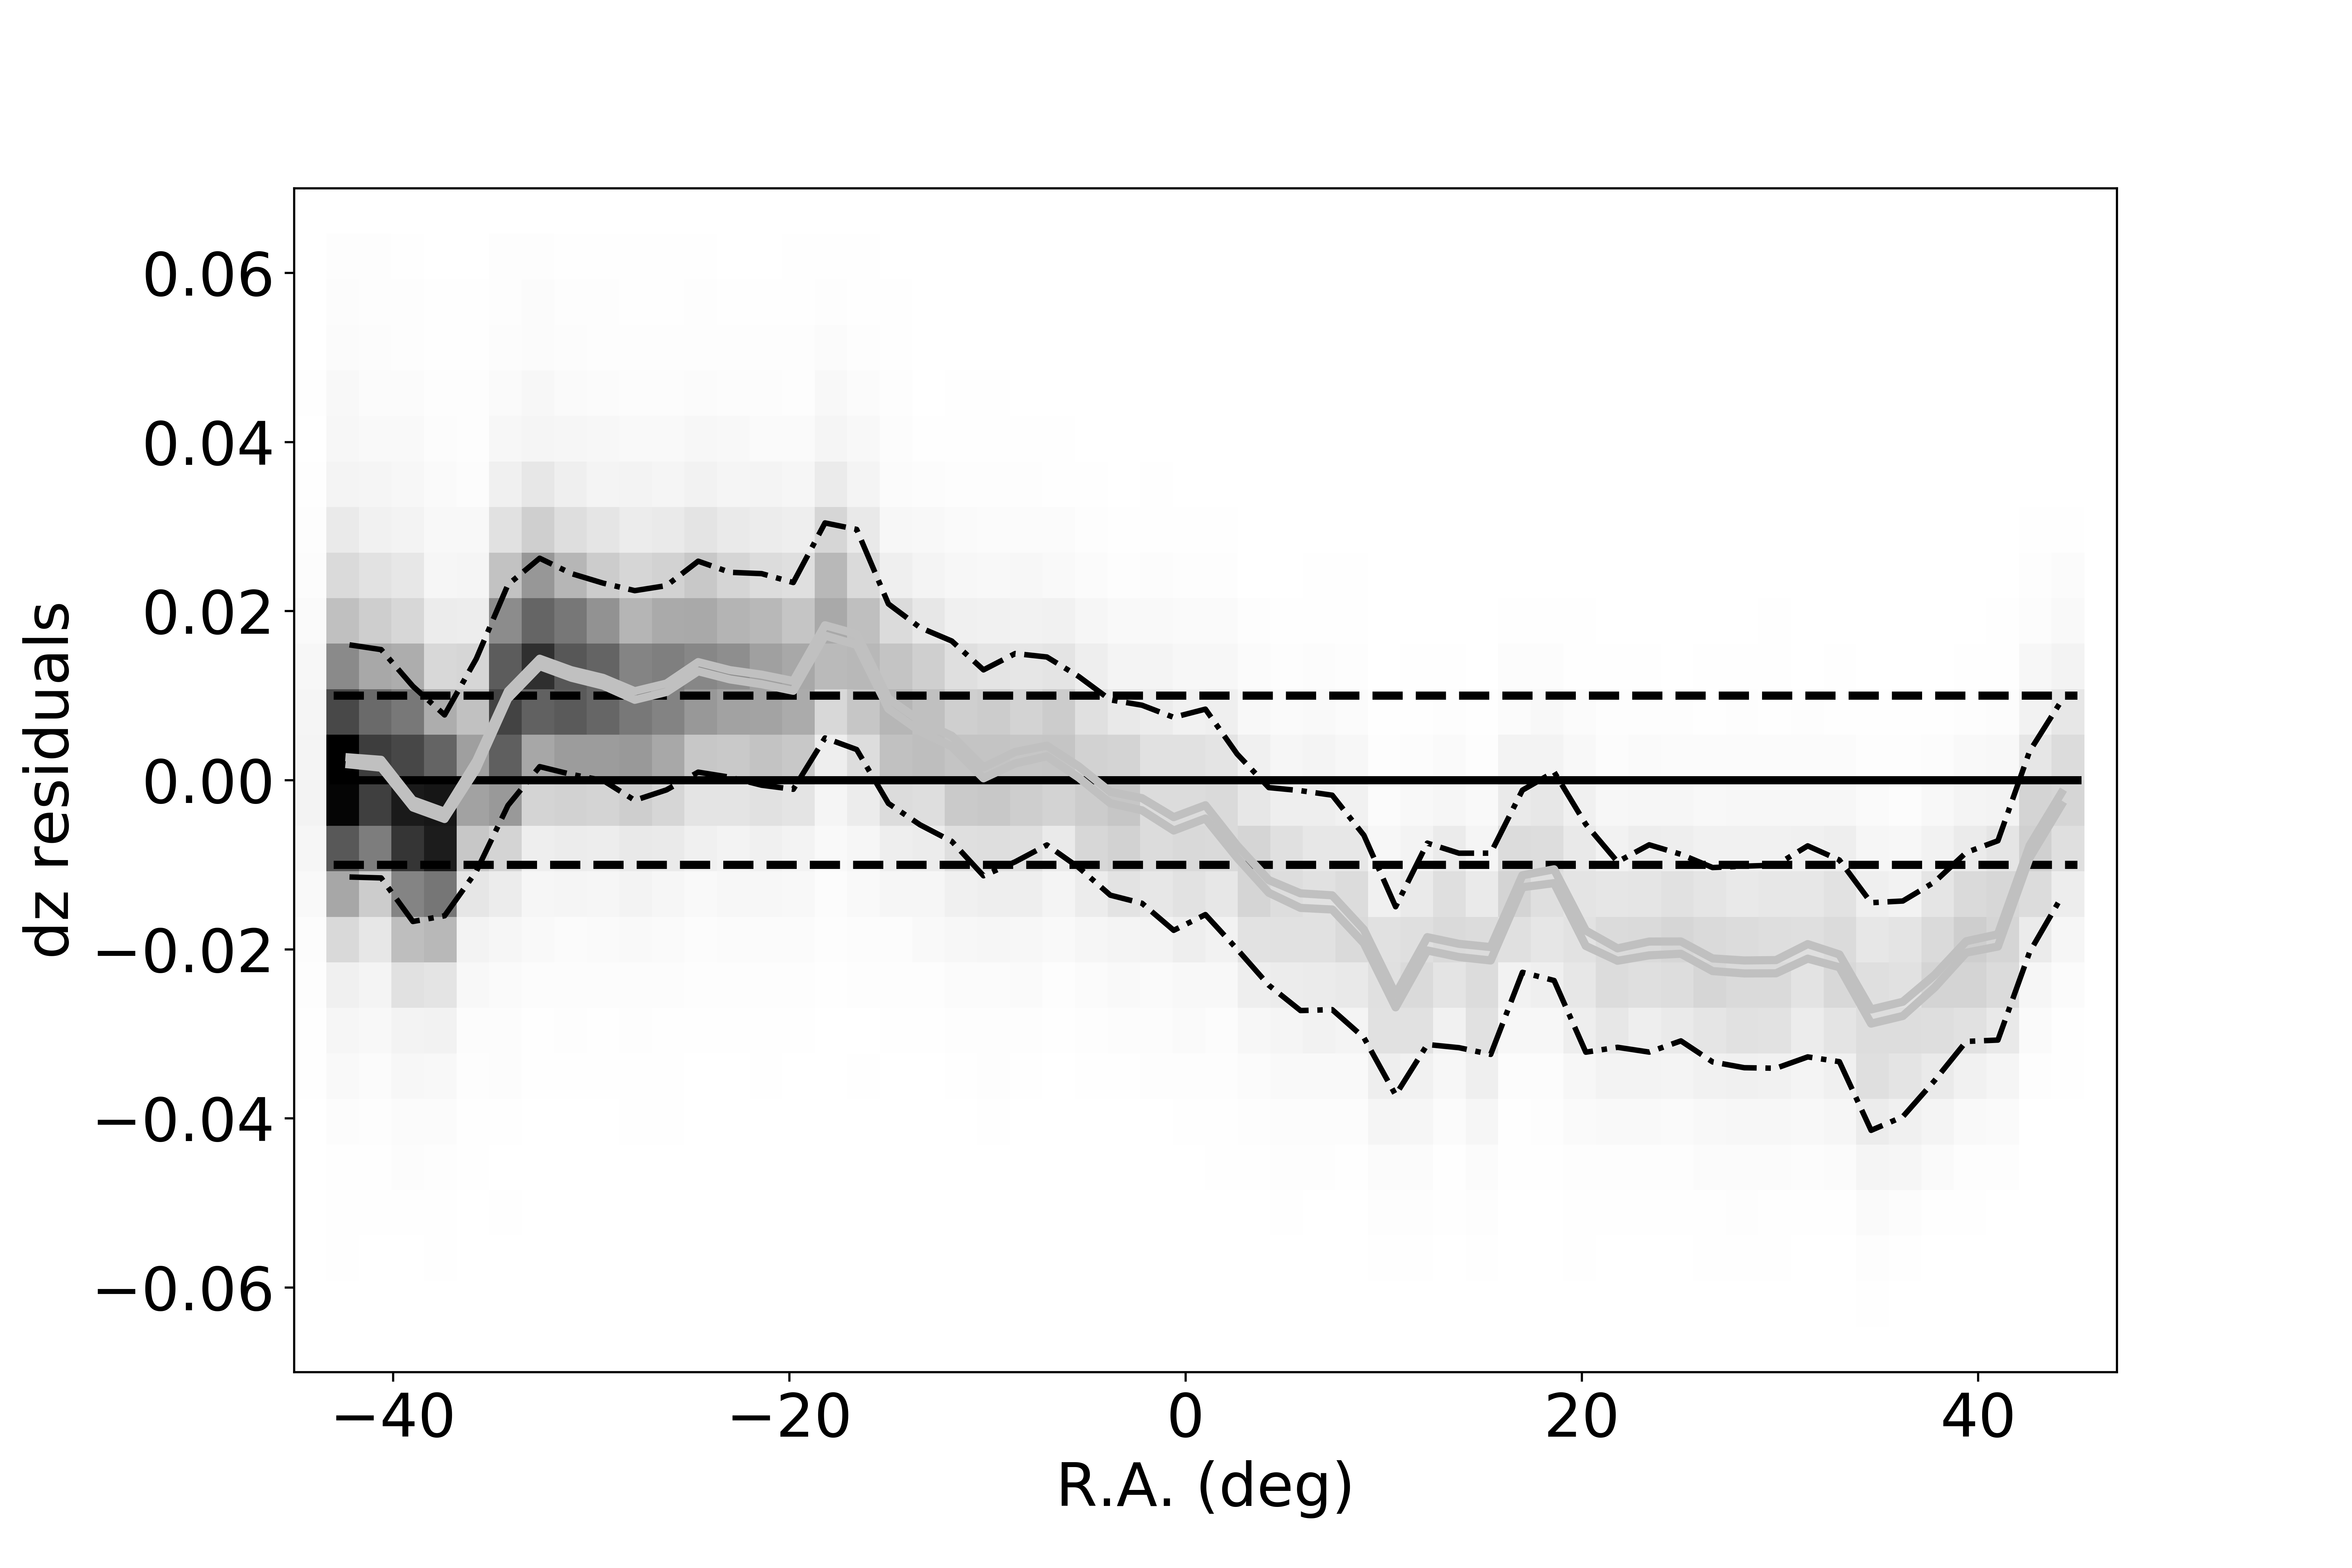
\includegraphics[width=7cm]{figures/colorResidDES2bright_dz_RA_Hess.png}
    \centering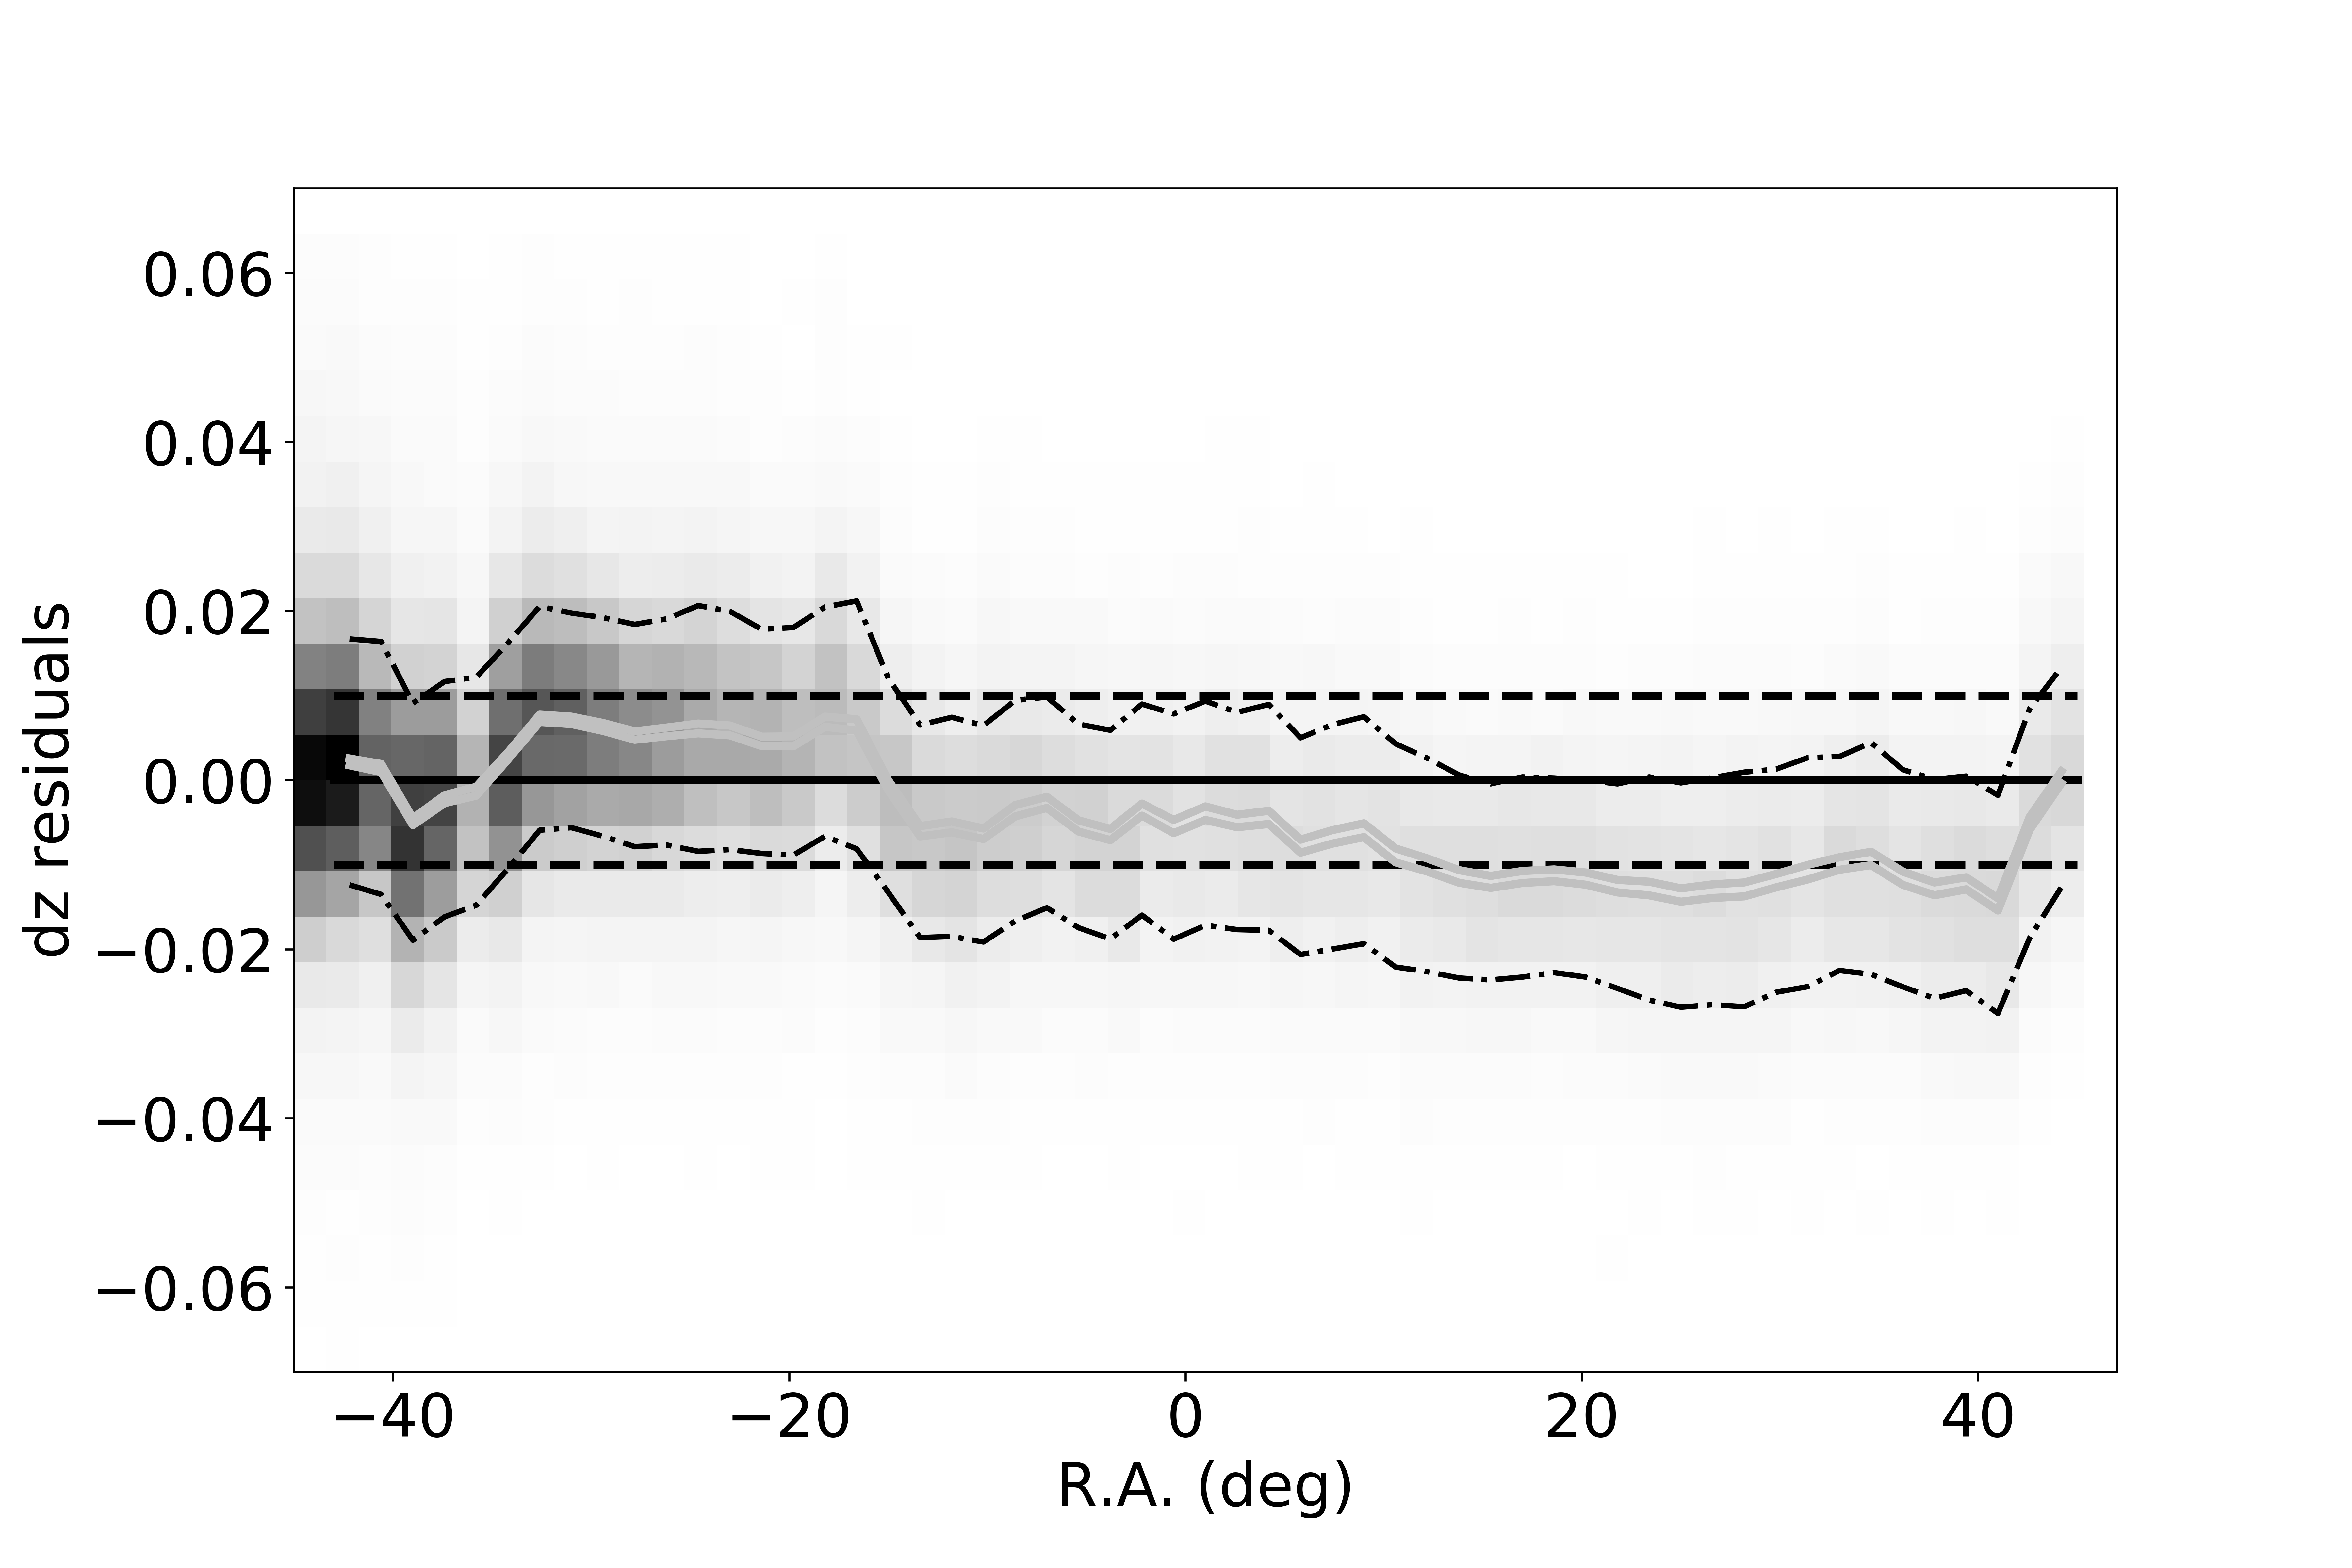
\includegraphics[width=7cm]{figures/colorResidPSbright_dz_RA_Hess.png}
\caption{A comparison of the magnitude differences between the SDSS v3.4 catalog
and DES (left) and Pan-STARRS (right) catalogs, for the $riz$ bands.}
\label{fig:DESPSRA}
\end{figure}

\begin{figure}[th!]
    \centering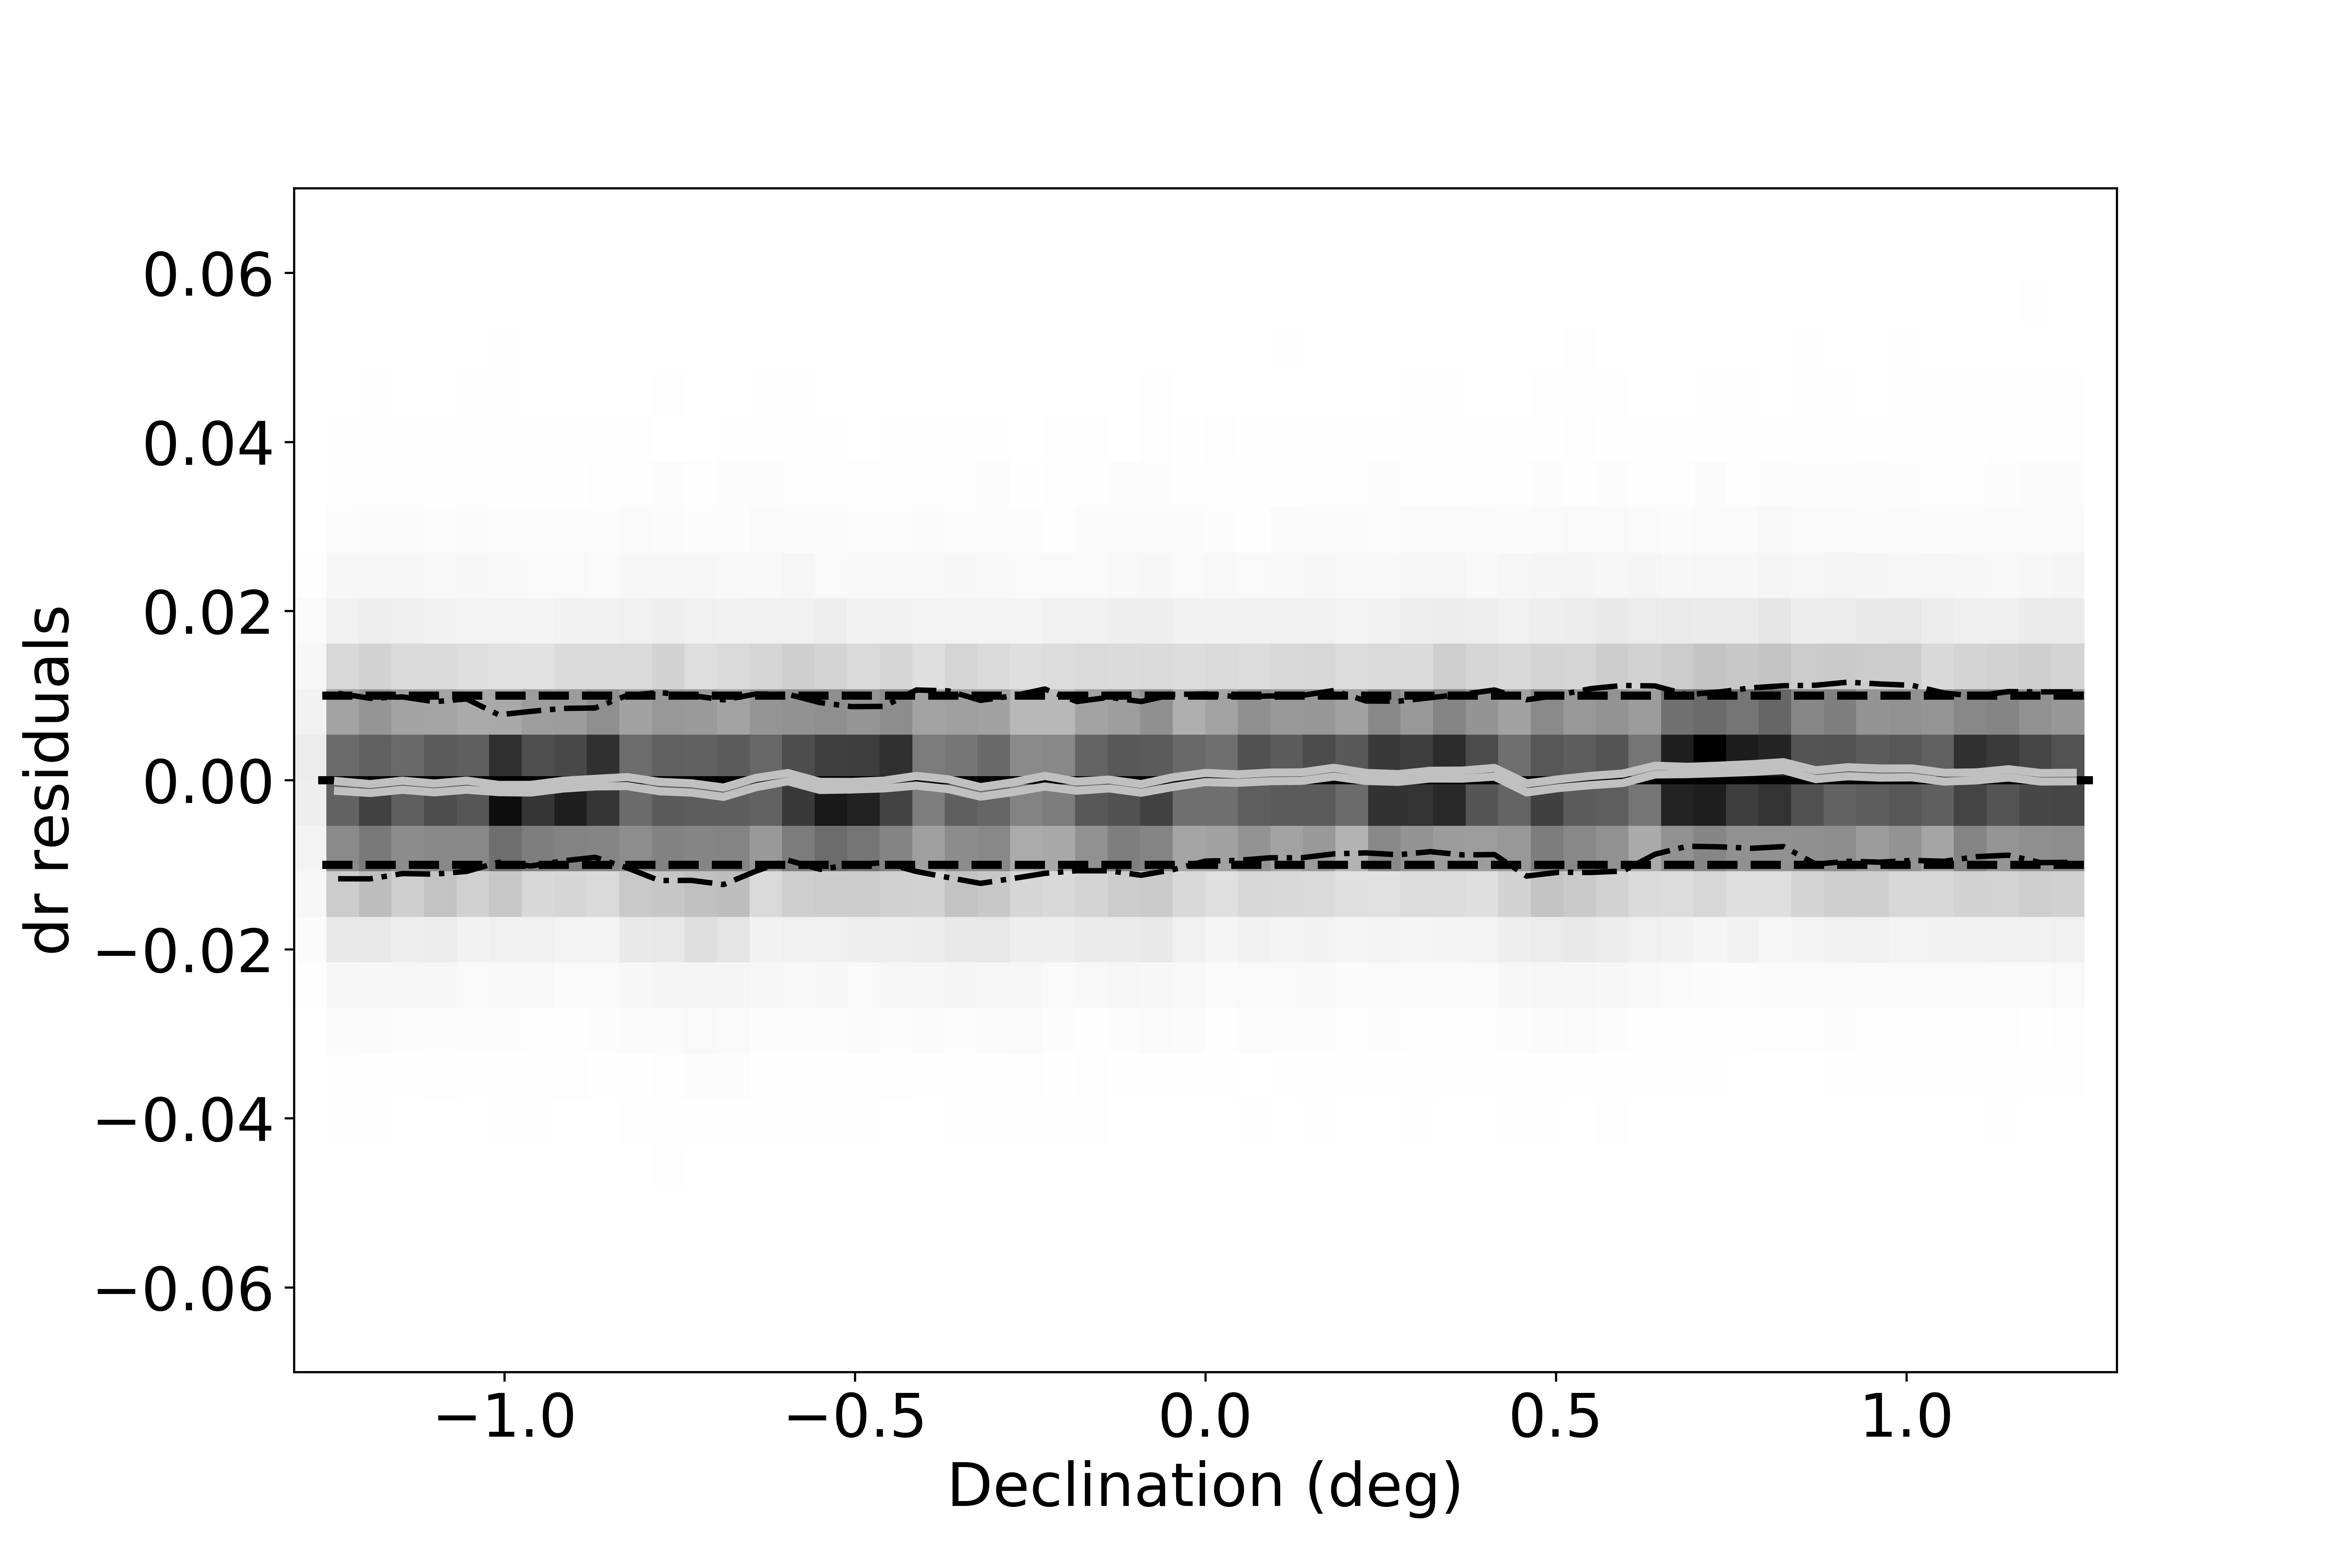
\includegraphics[width=7cm]{figures/colorResidDES2bright_dr_Dec_Hess.png}
    \centering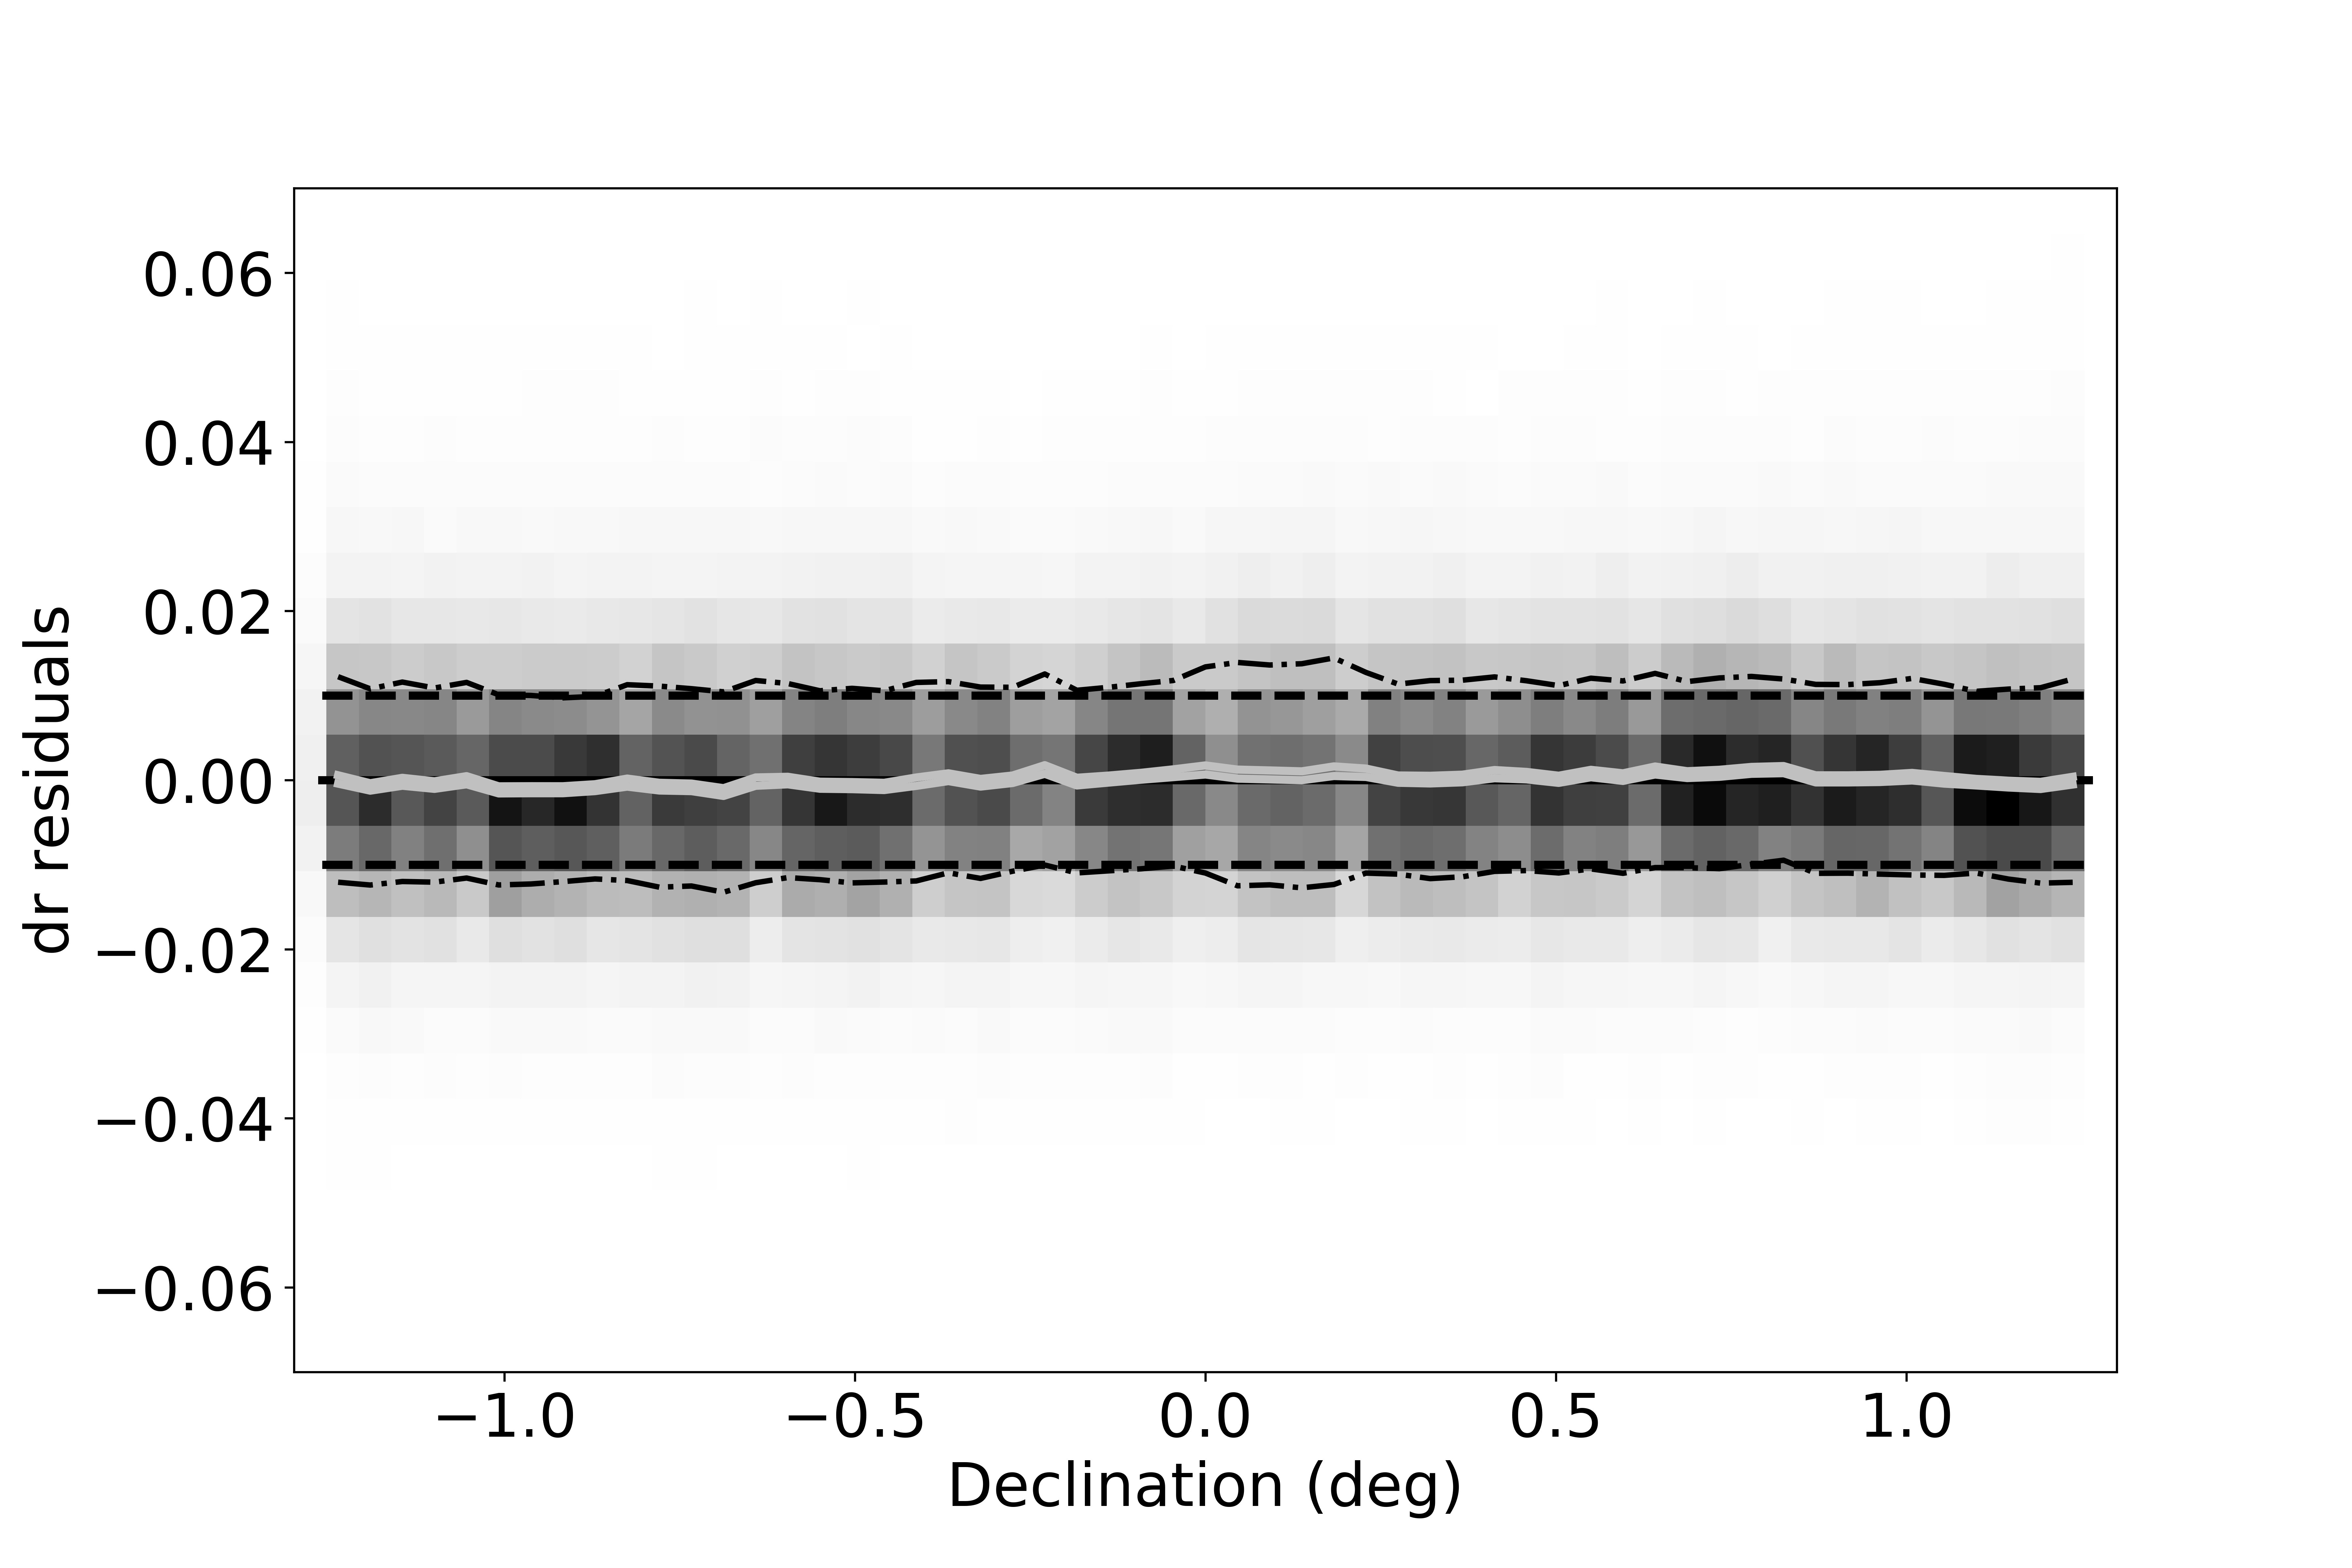
\includegraphics[width=7cm]{figures/colorResidPSbright_dr_Dec_Hess.png}
    \centering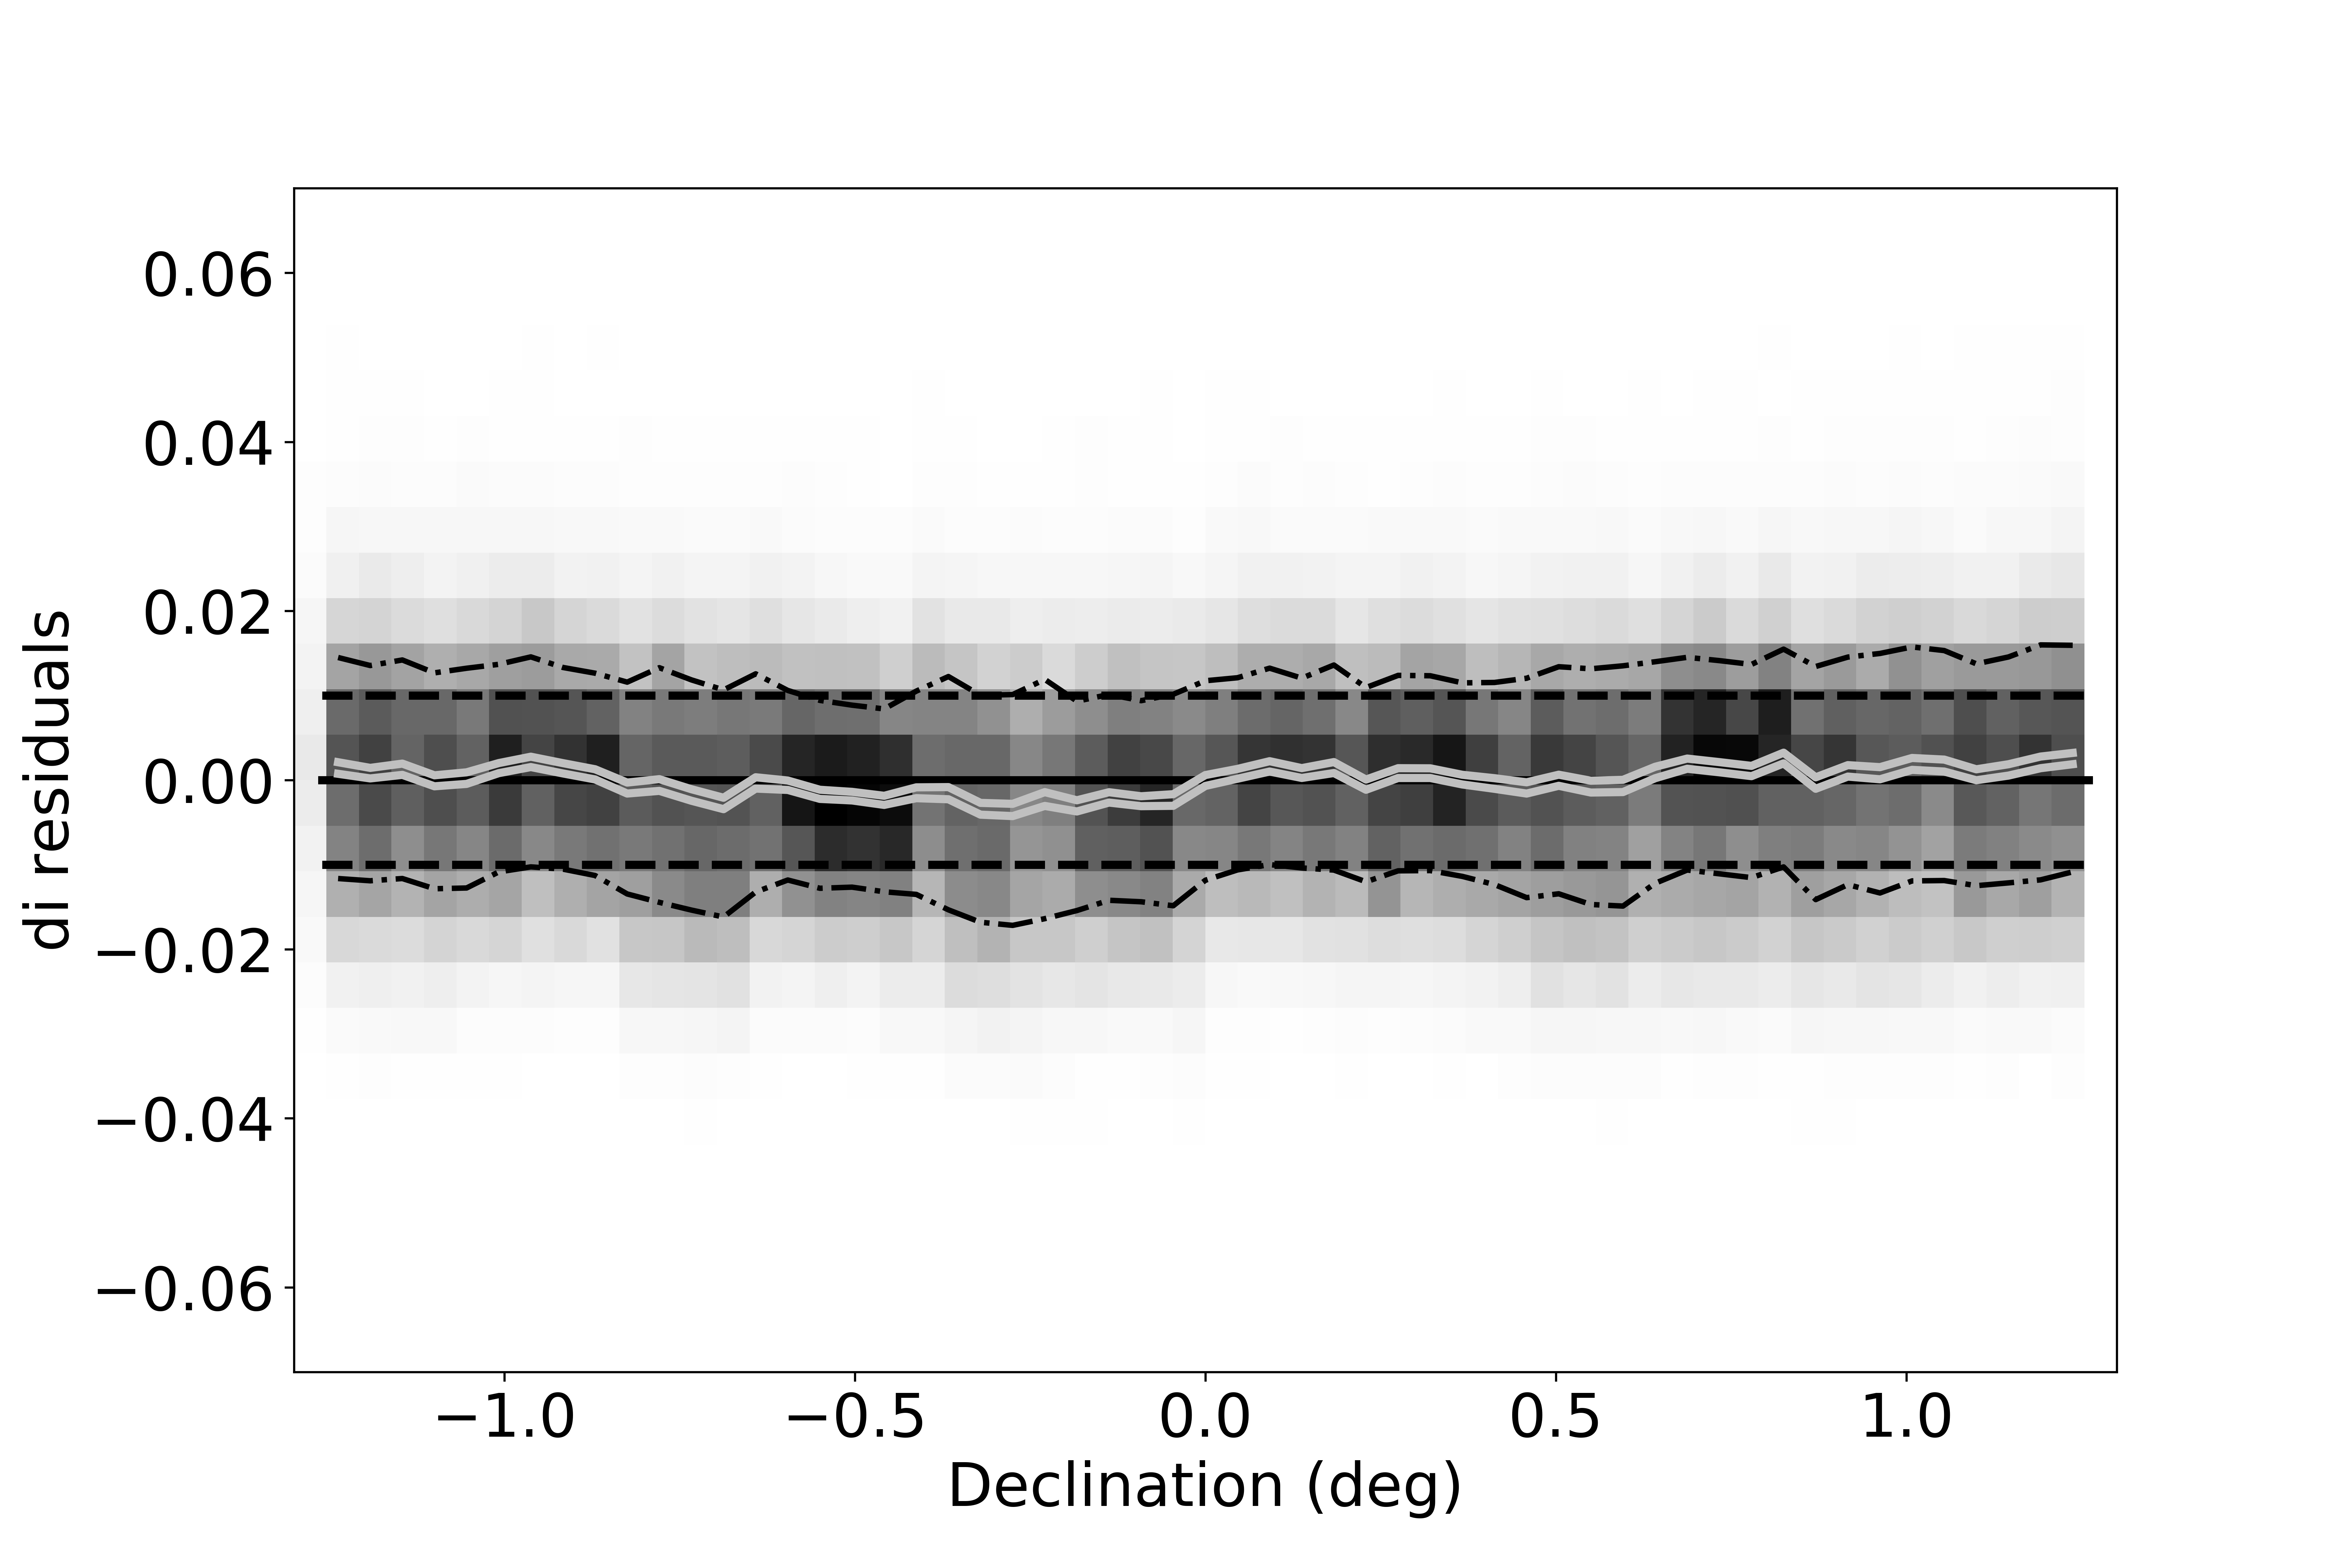
\includegraphics[width=7cm]{figures/colorResidDES2bright_di_Dec_Hess.png}
    \centering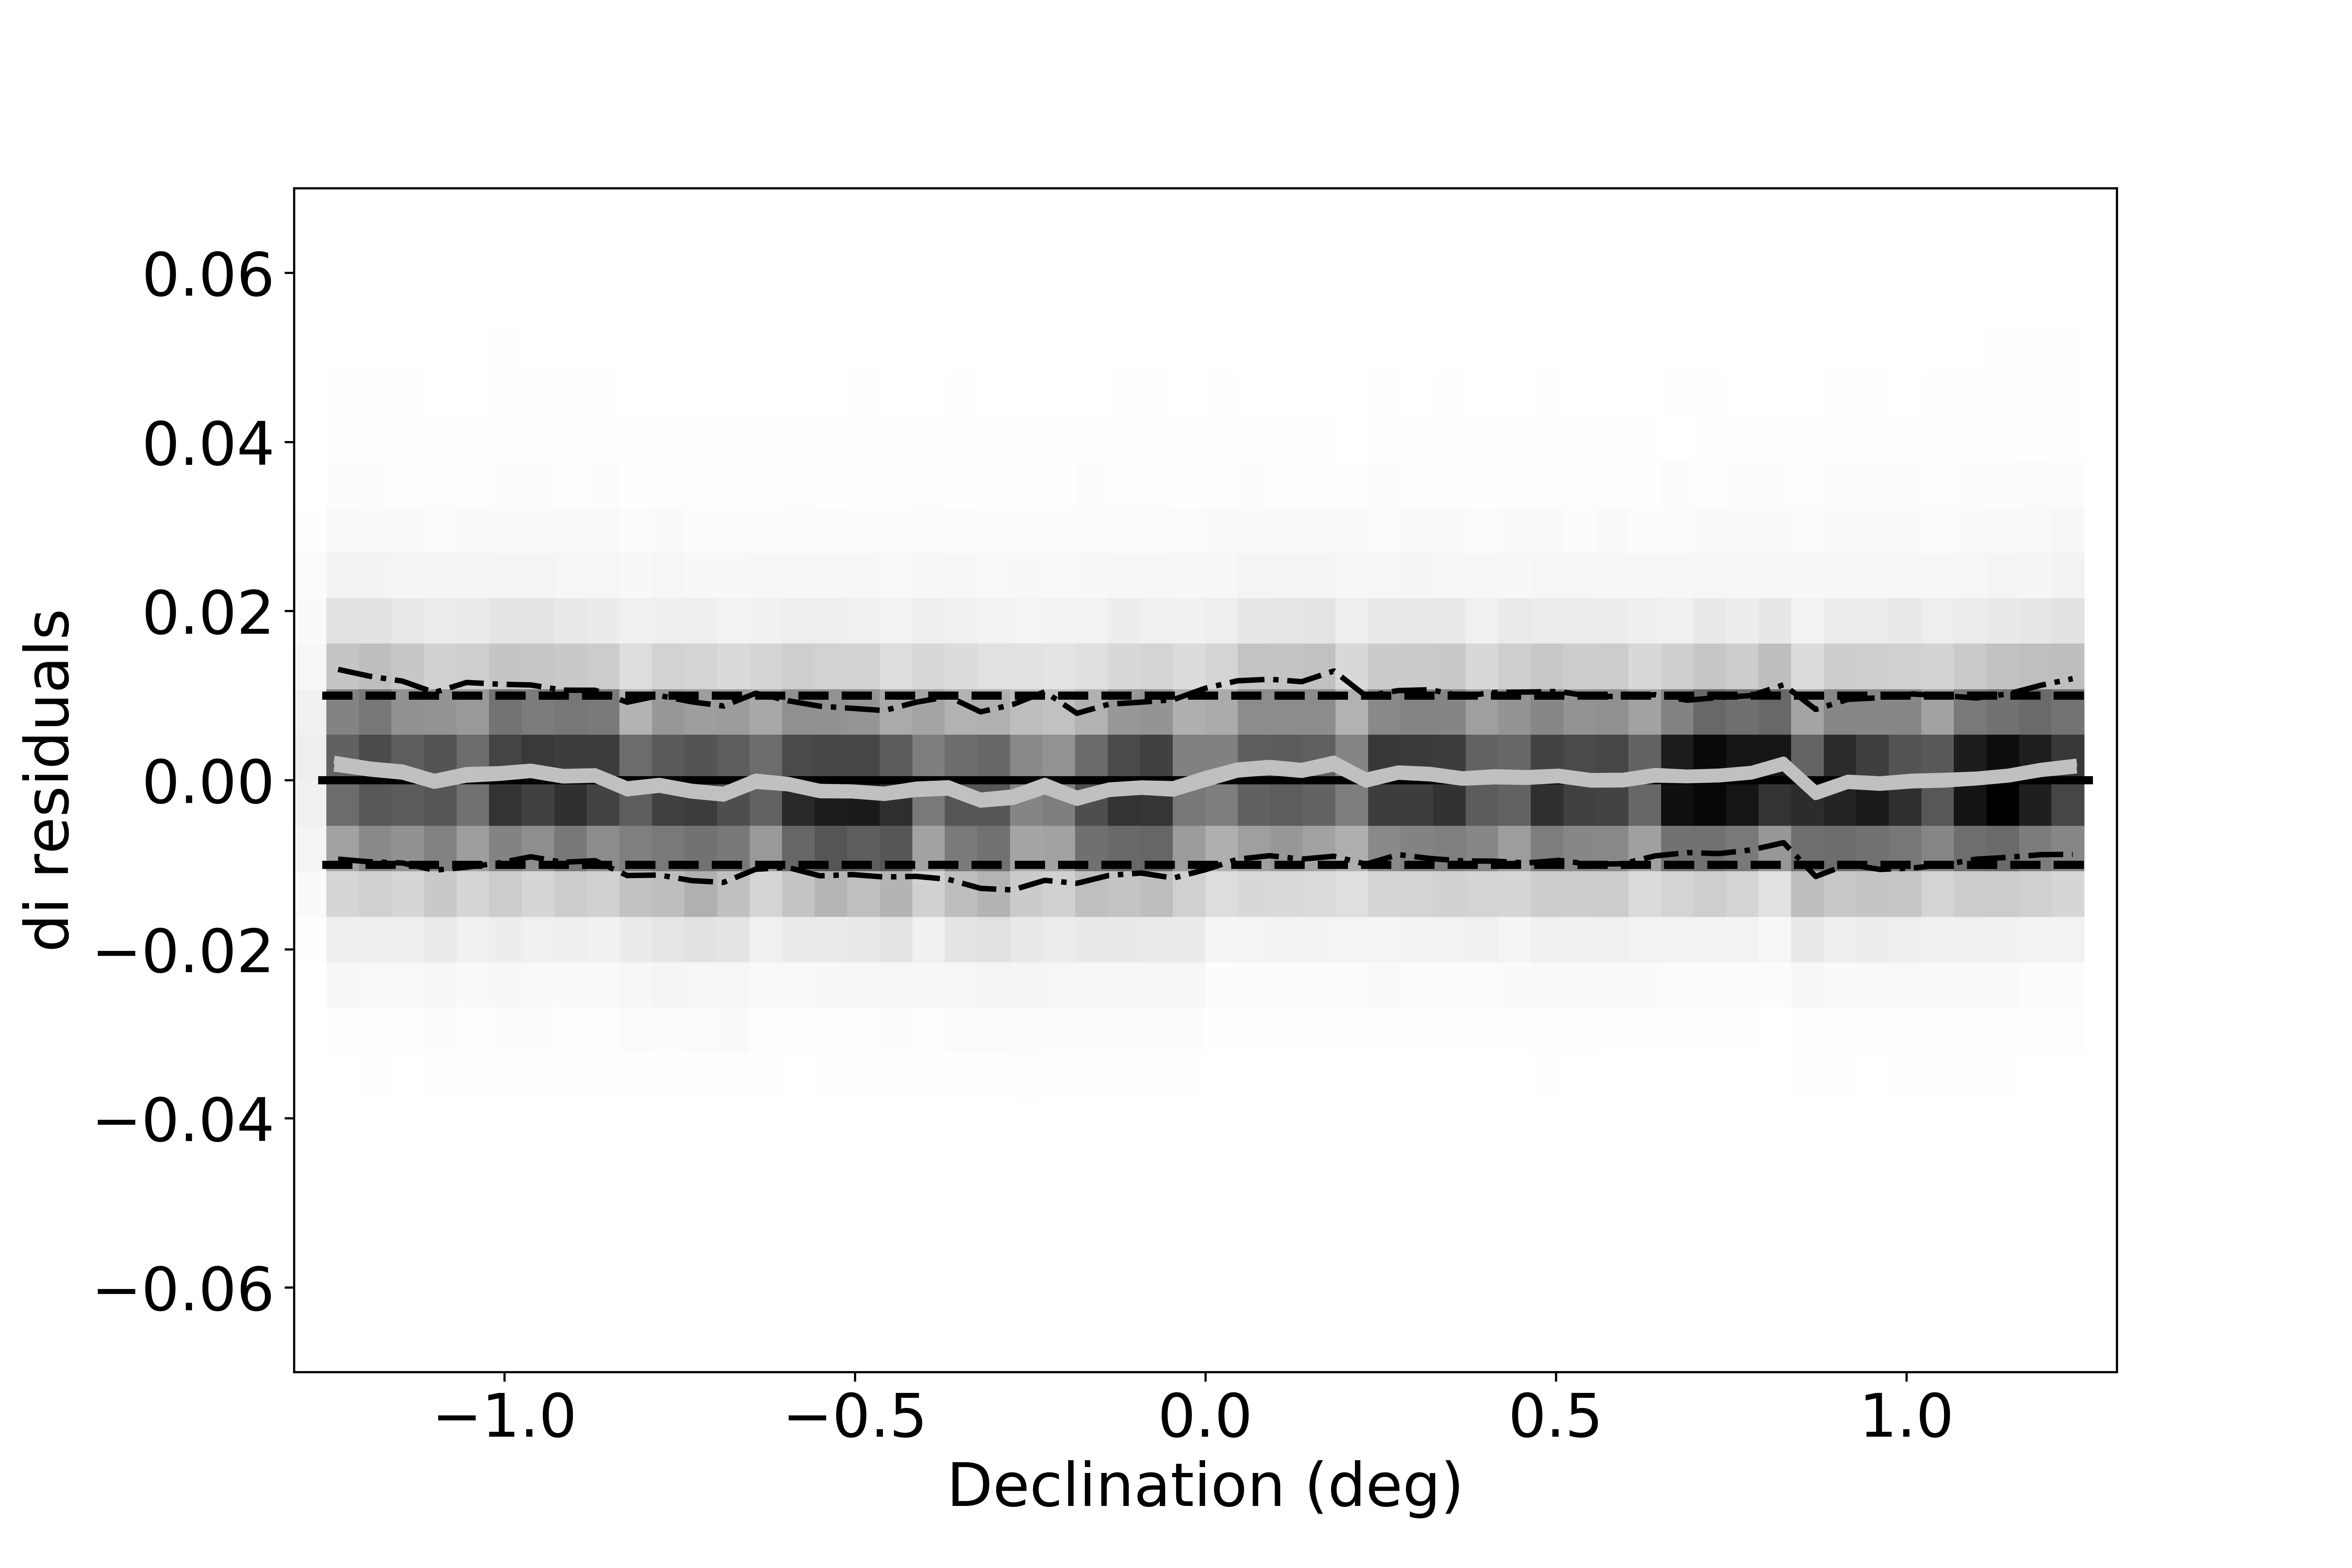
\includegraphics[width=7cm]{figures/colorResidPSbright_di_Dec_Hess.png}
    \centering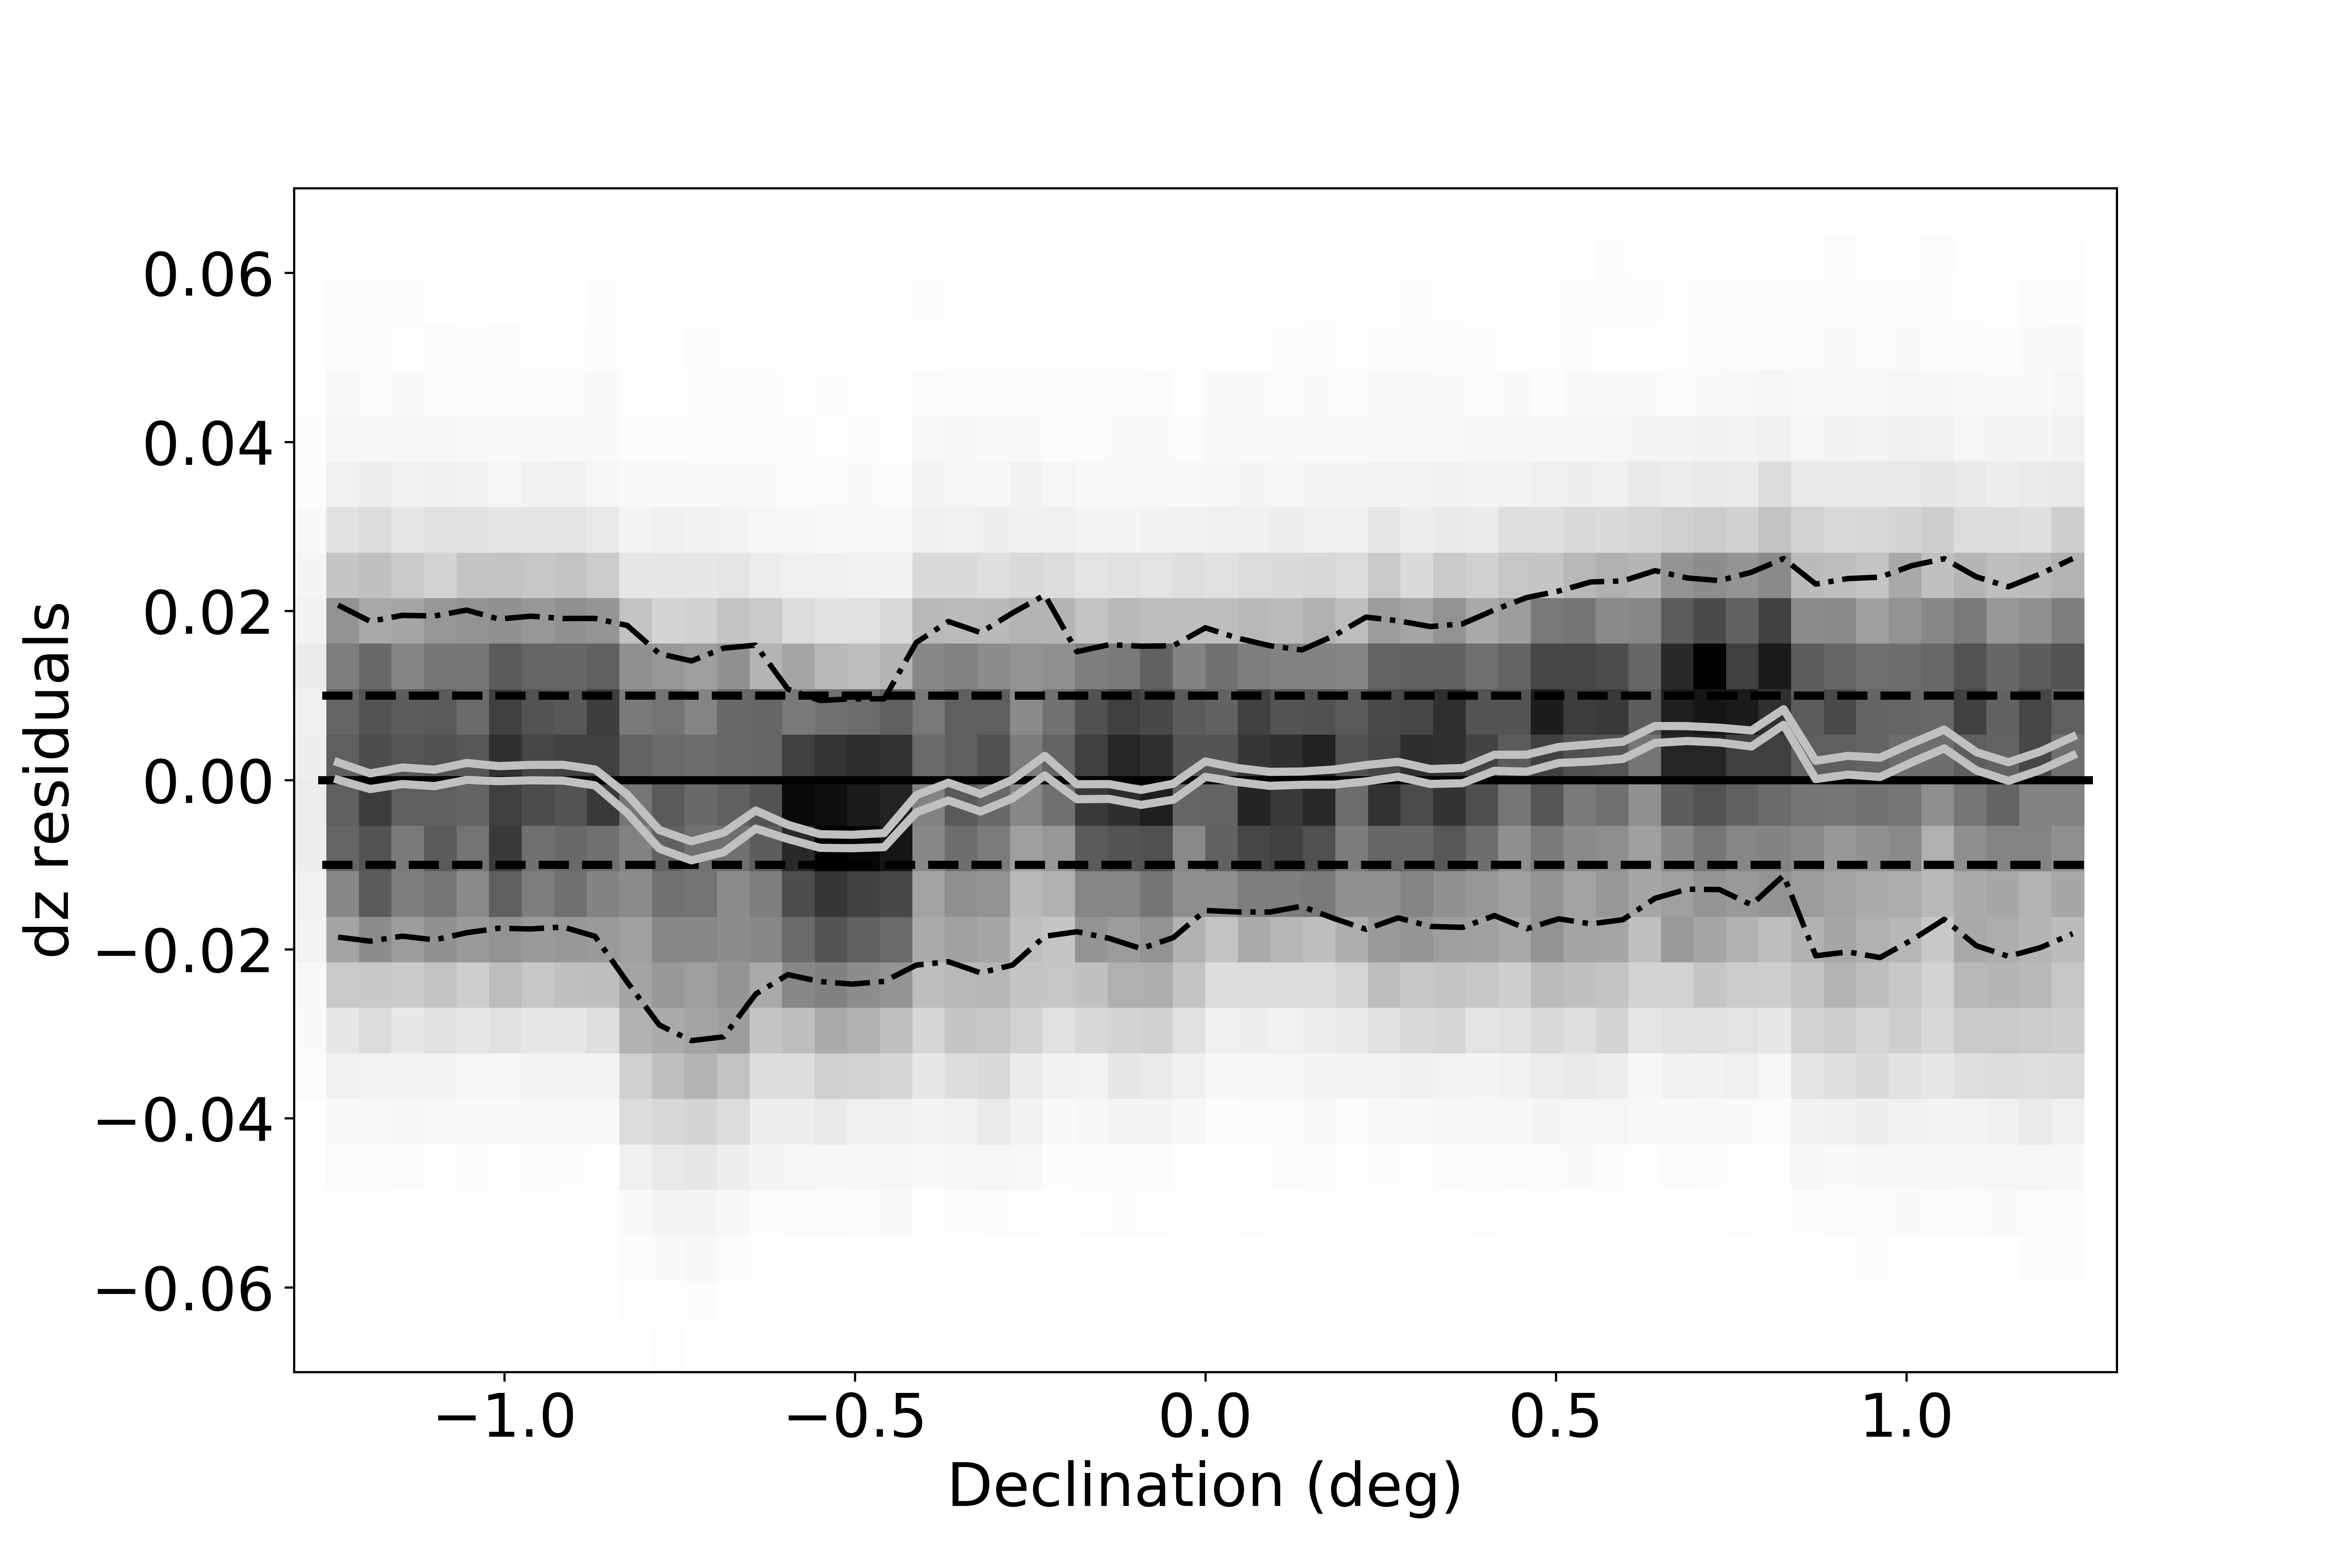
\includegraphics[width=7cm]{figures/colorResidDES2bright_dz_Dec_Hess.png}
    \centering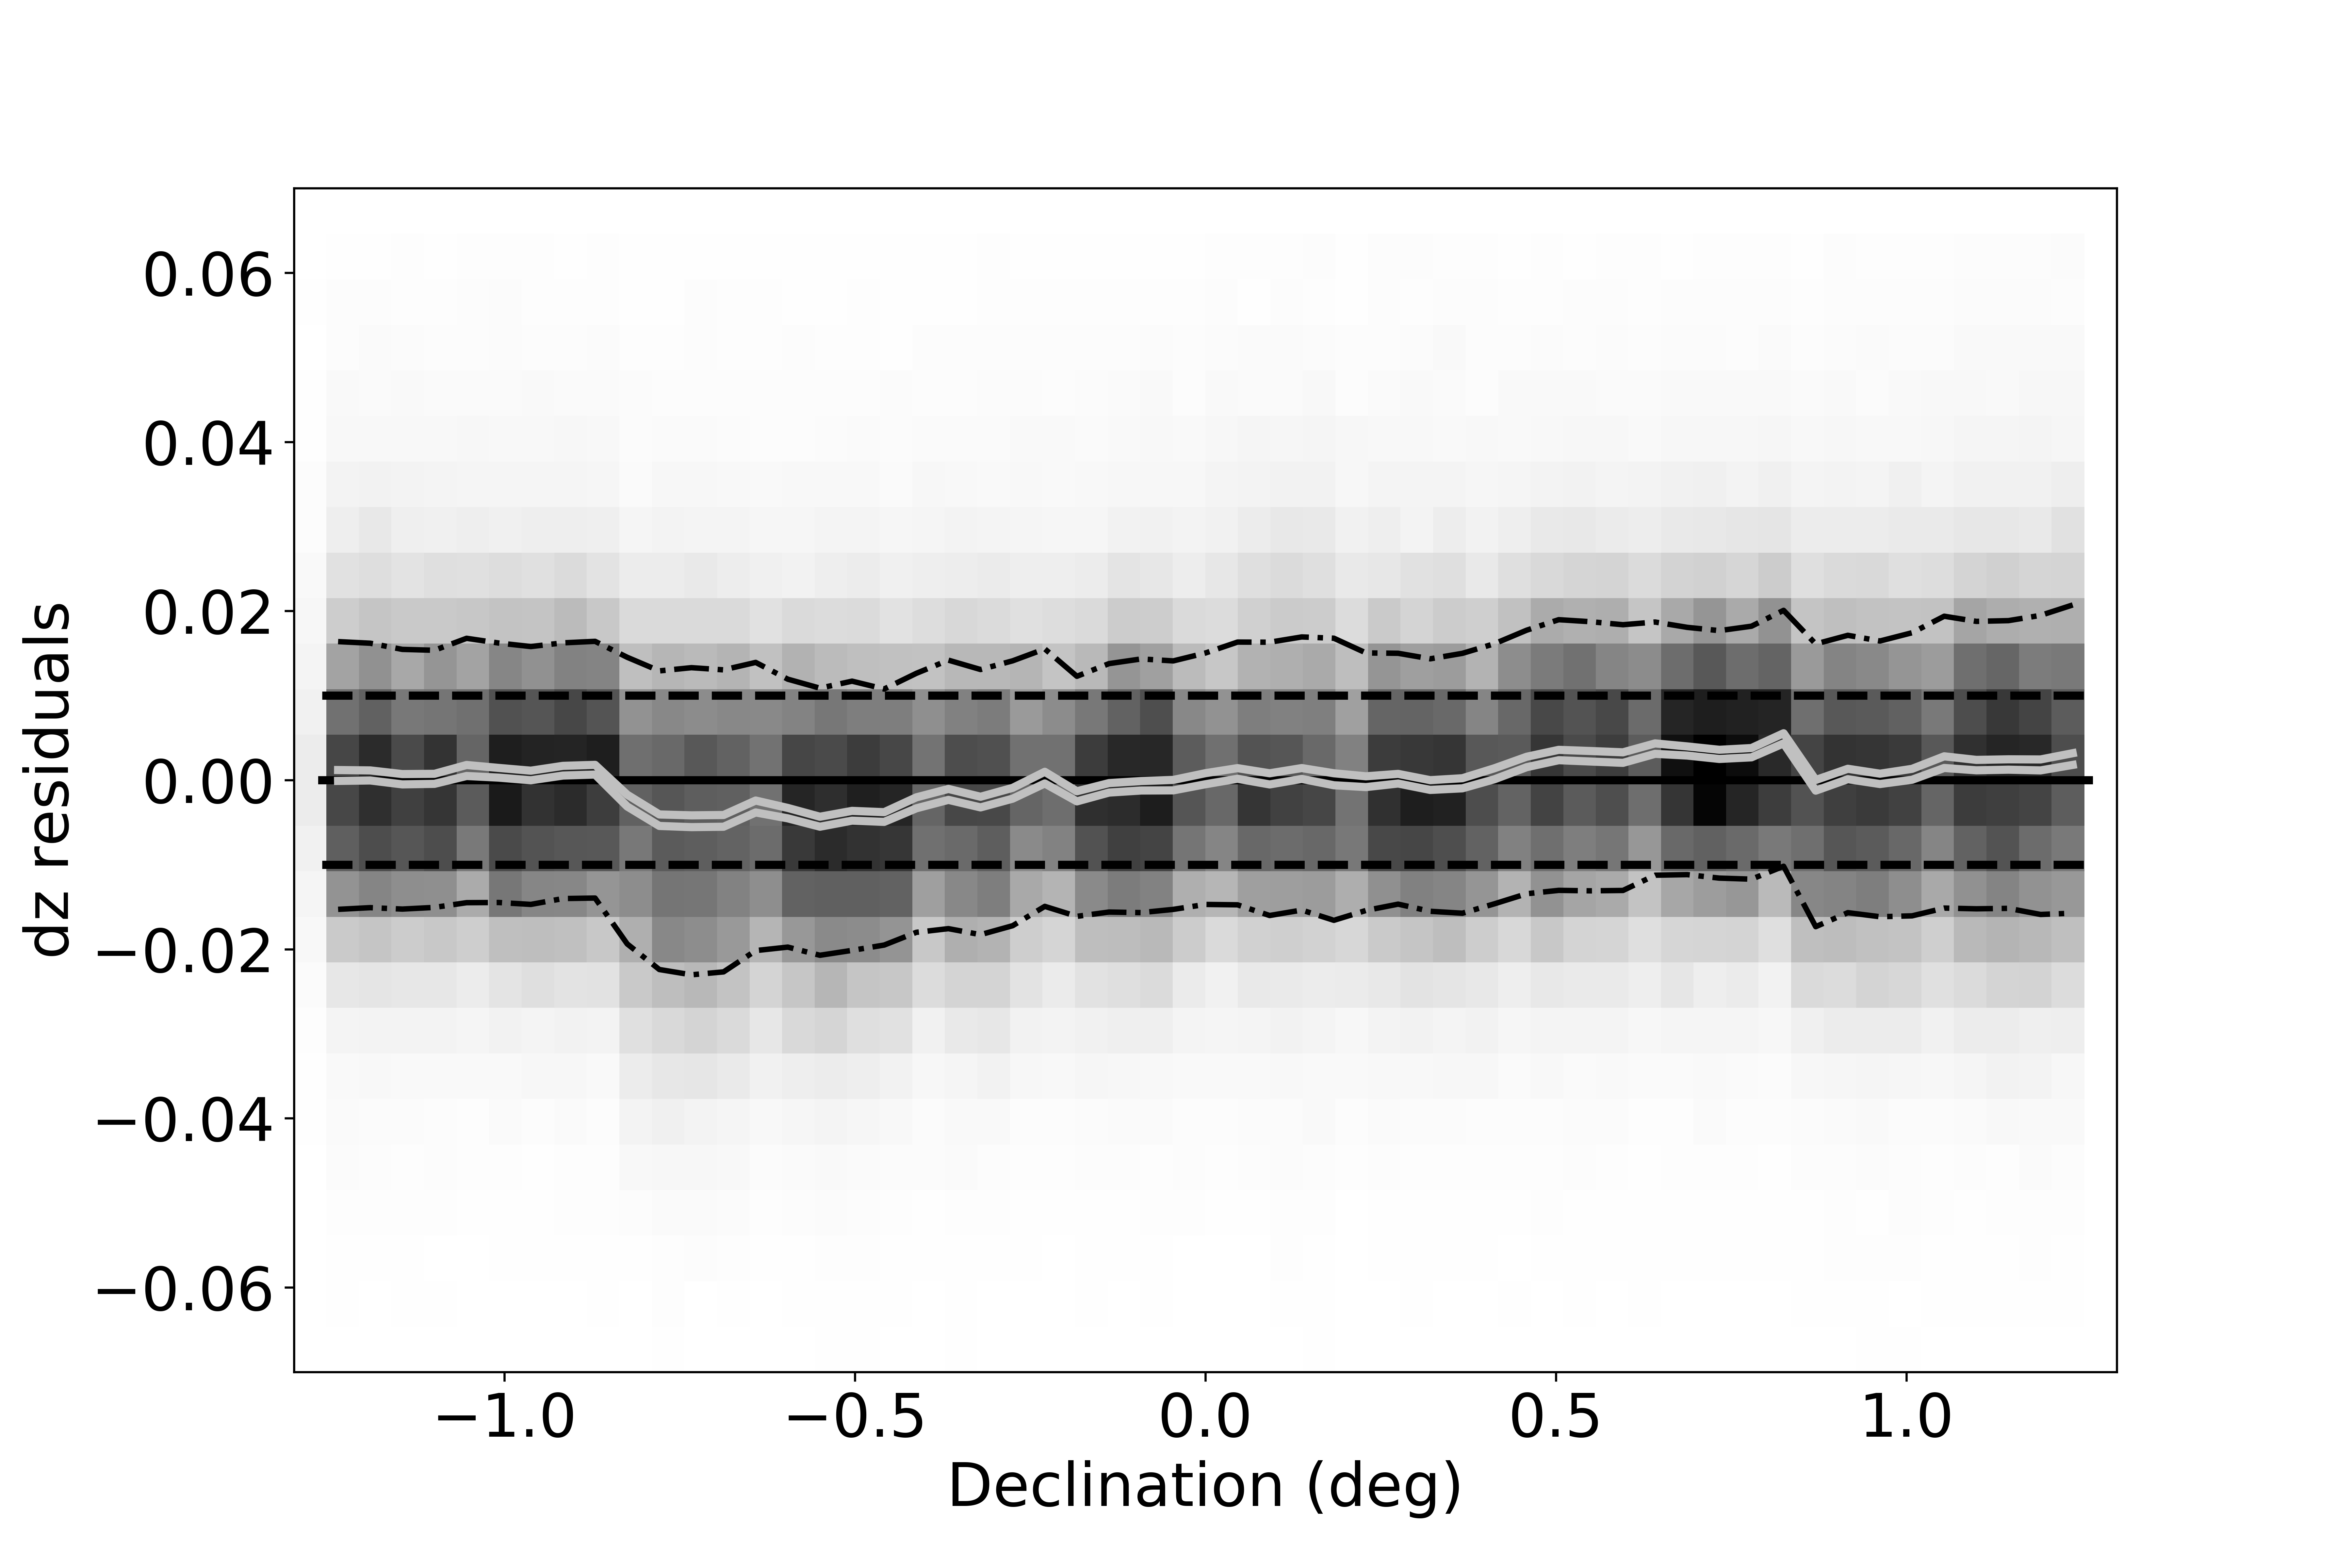
\includegraphics[width=7cm]{figures/colorResidPSbright_dz_Dec_Hess.png}
\caption{Analogous to Figure~\ref{fig:DESPSRA}, except that magnitude differences
are binned by Declination.}
\label{fig:DESPSDec}
\end{figure}

\begin{figure}[th!]
    \centering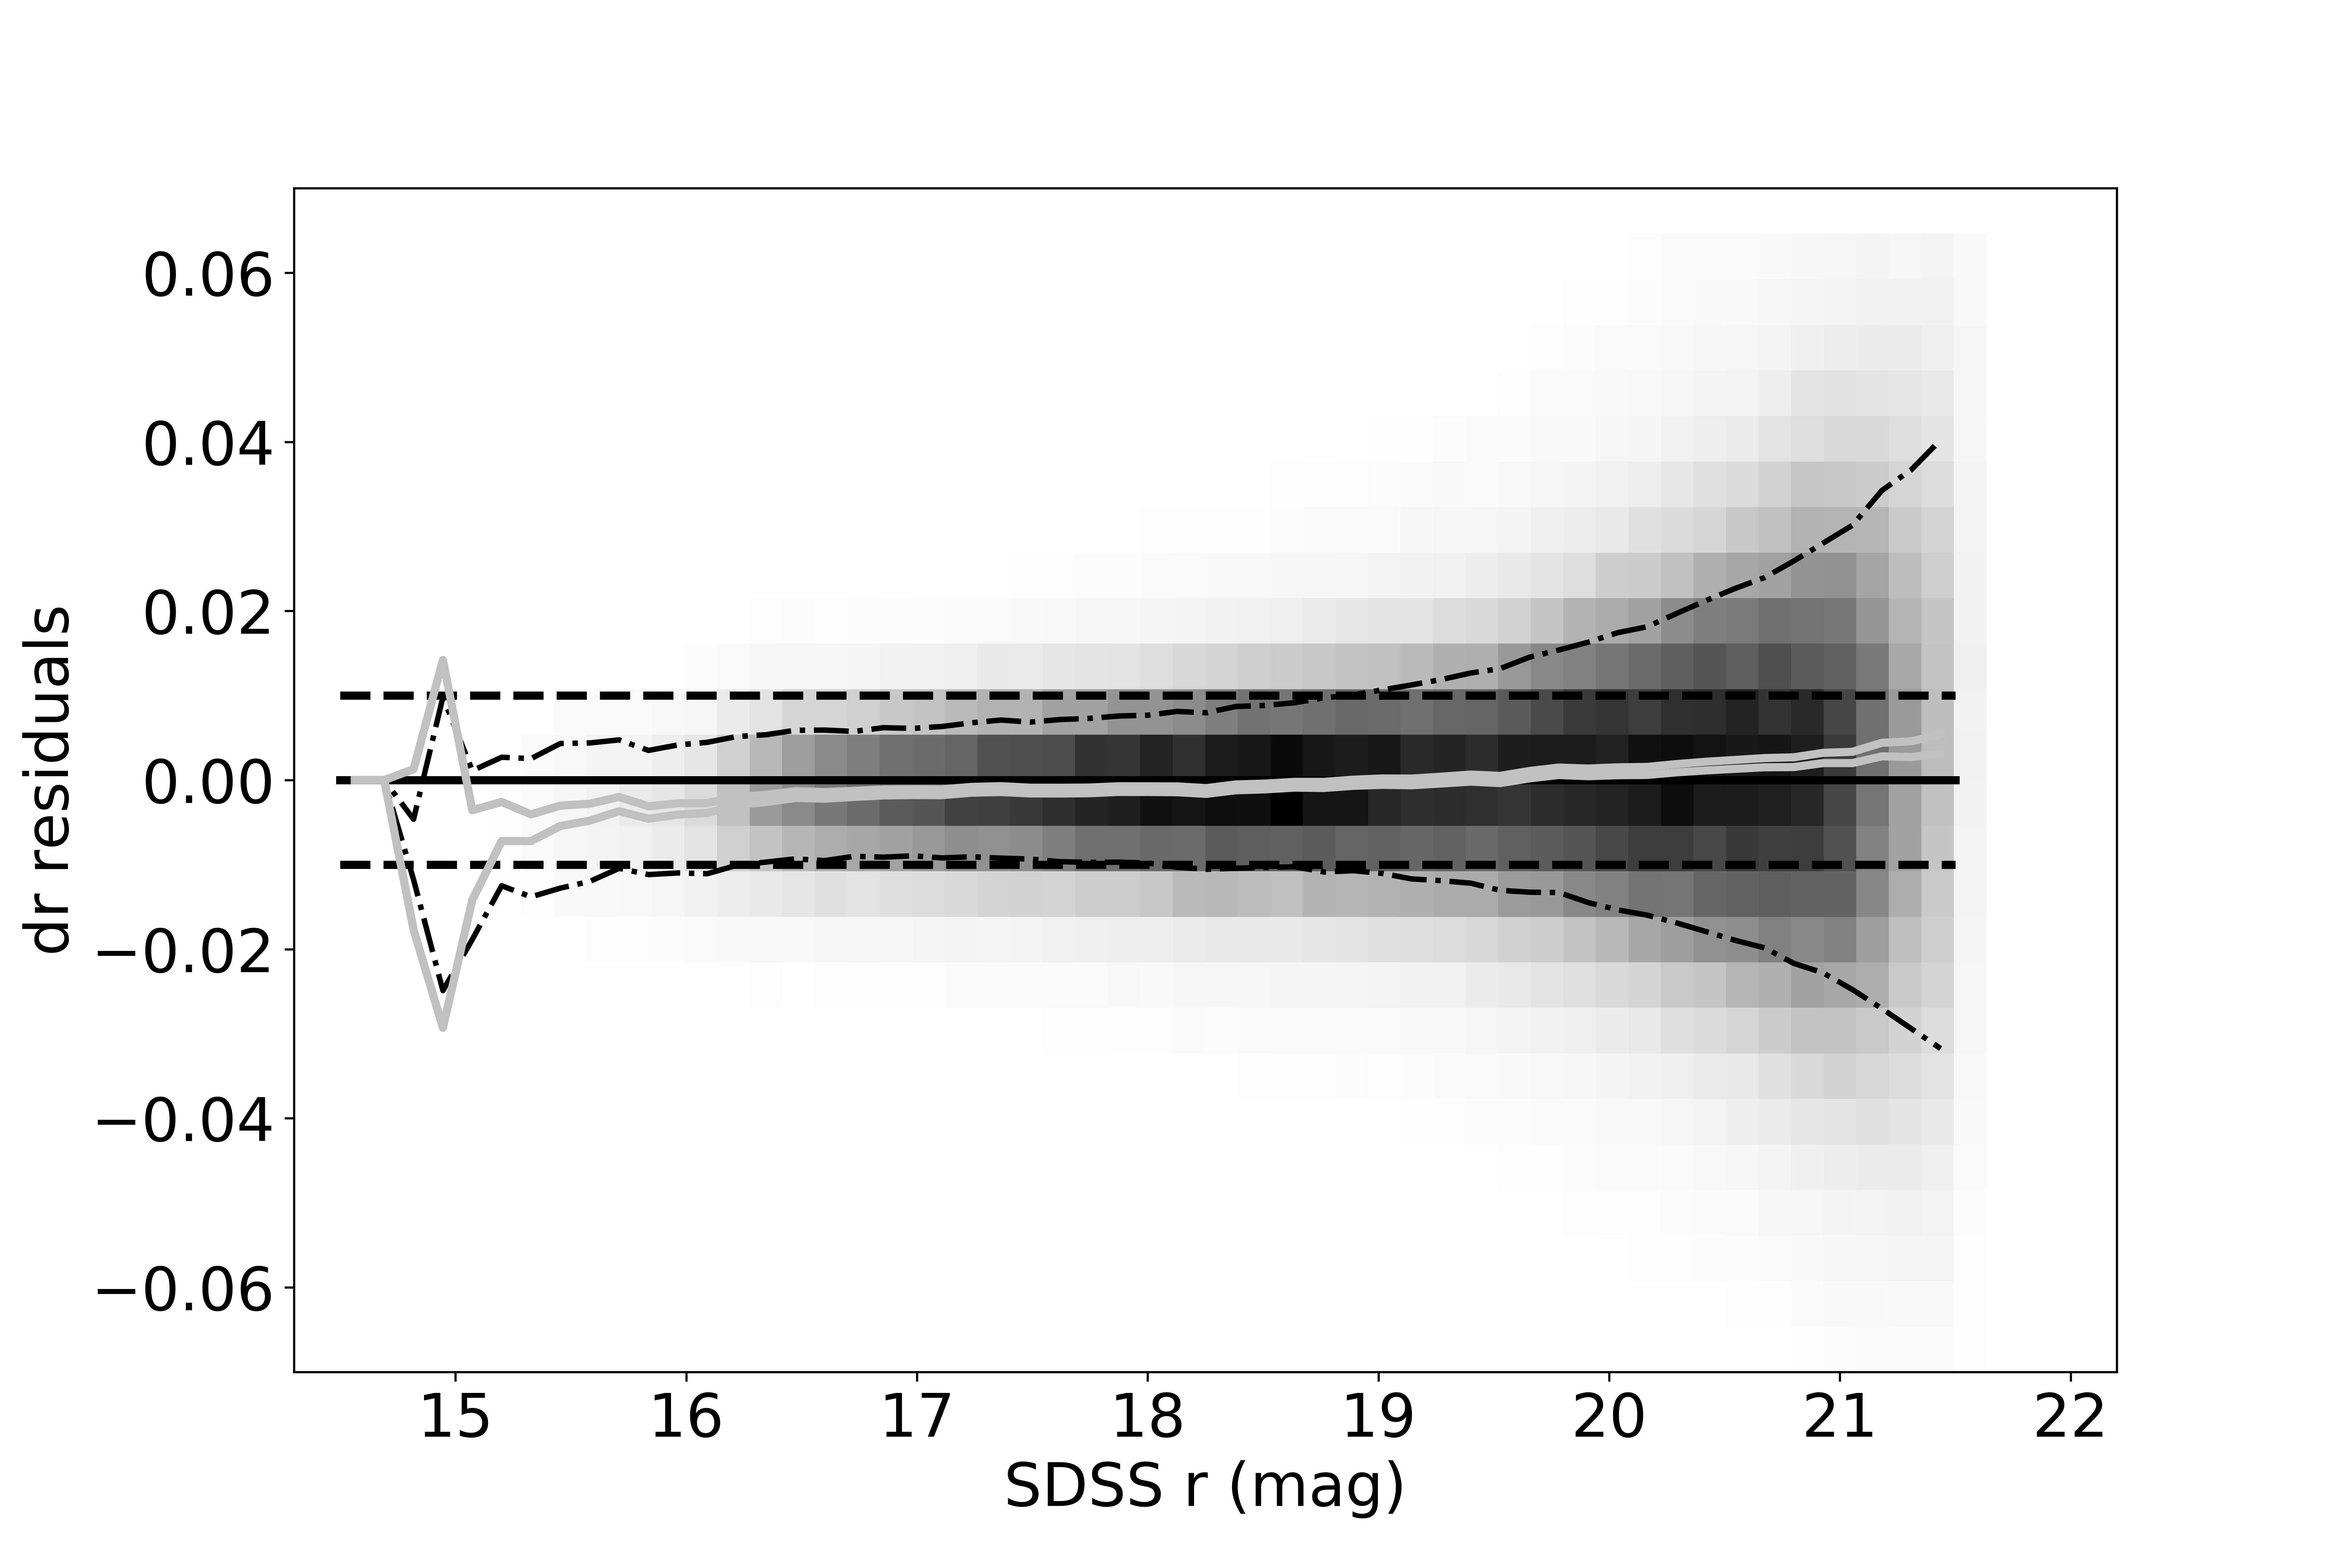
\includegraphics[width=7cm]{figures/colorResidDES2_dr_rmag_Hess.png}
    \centering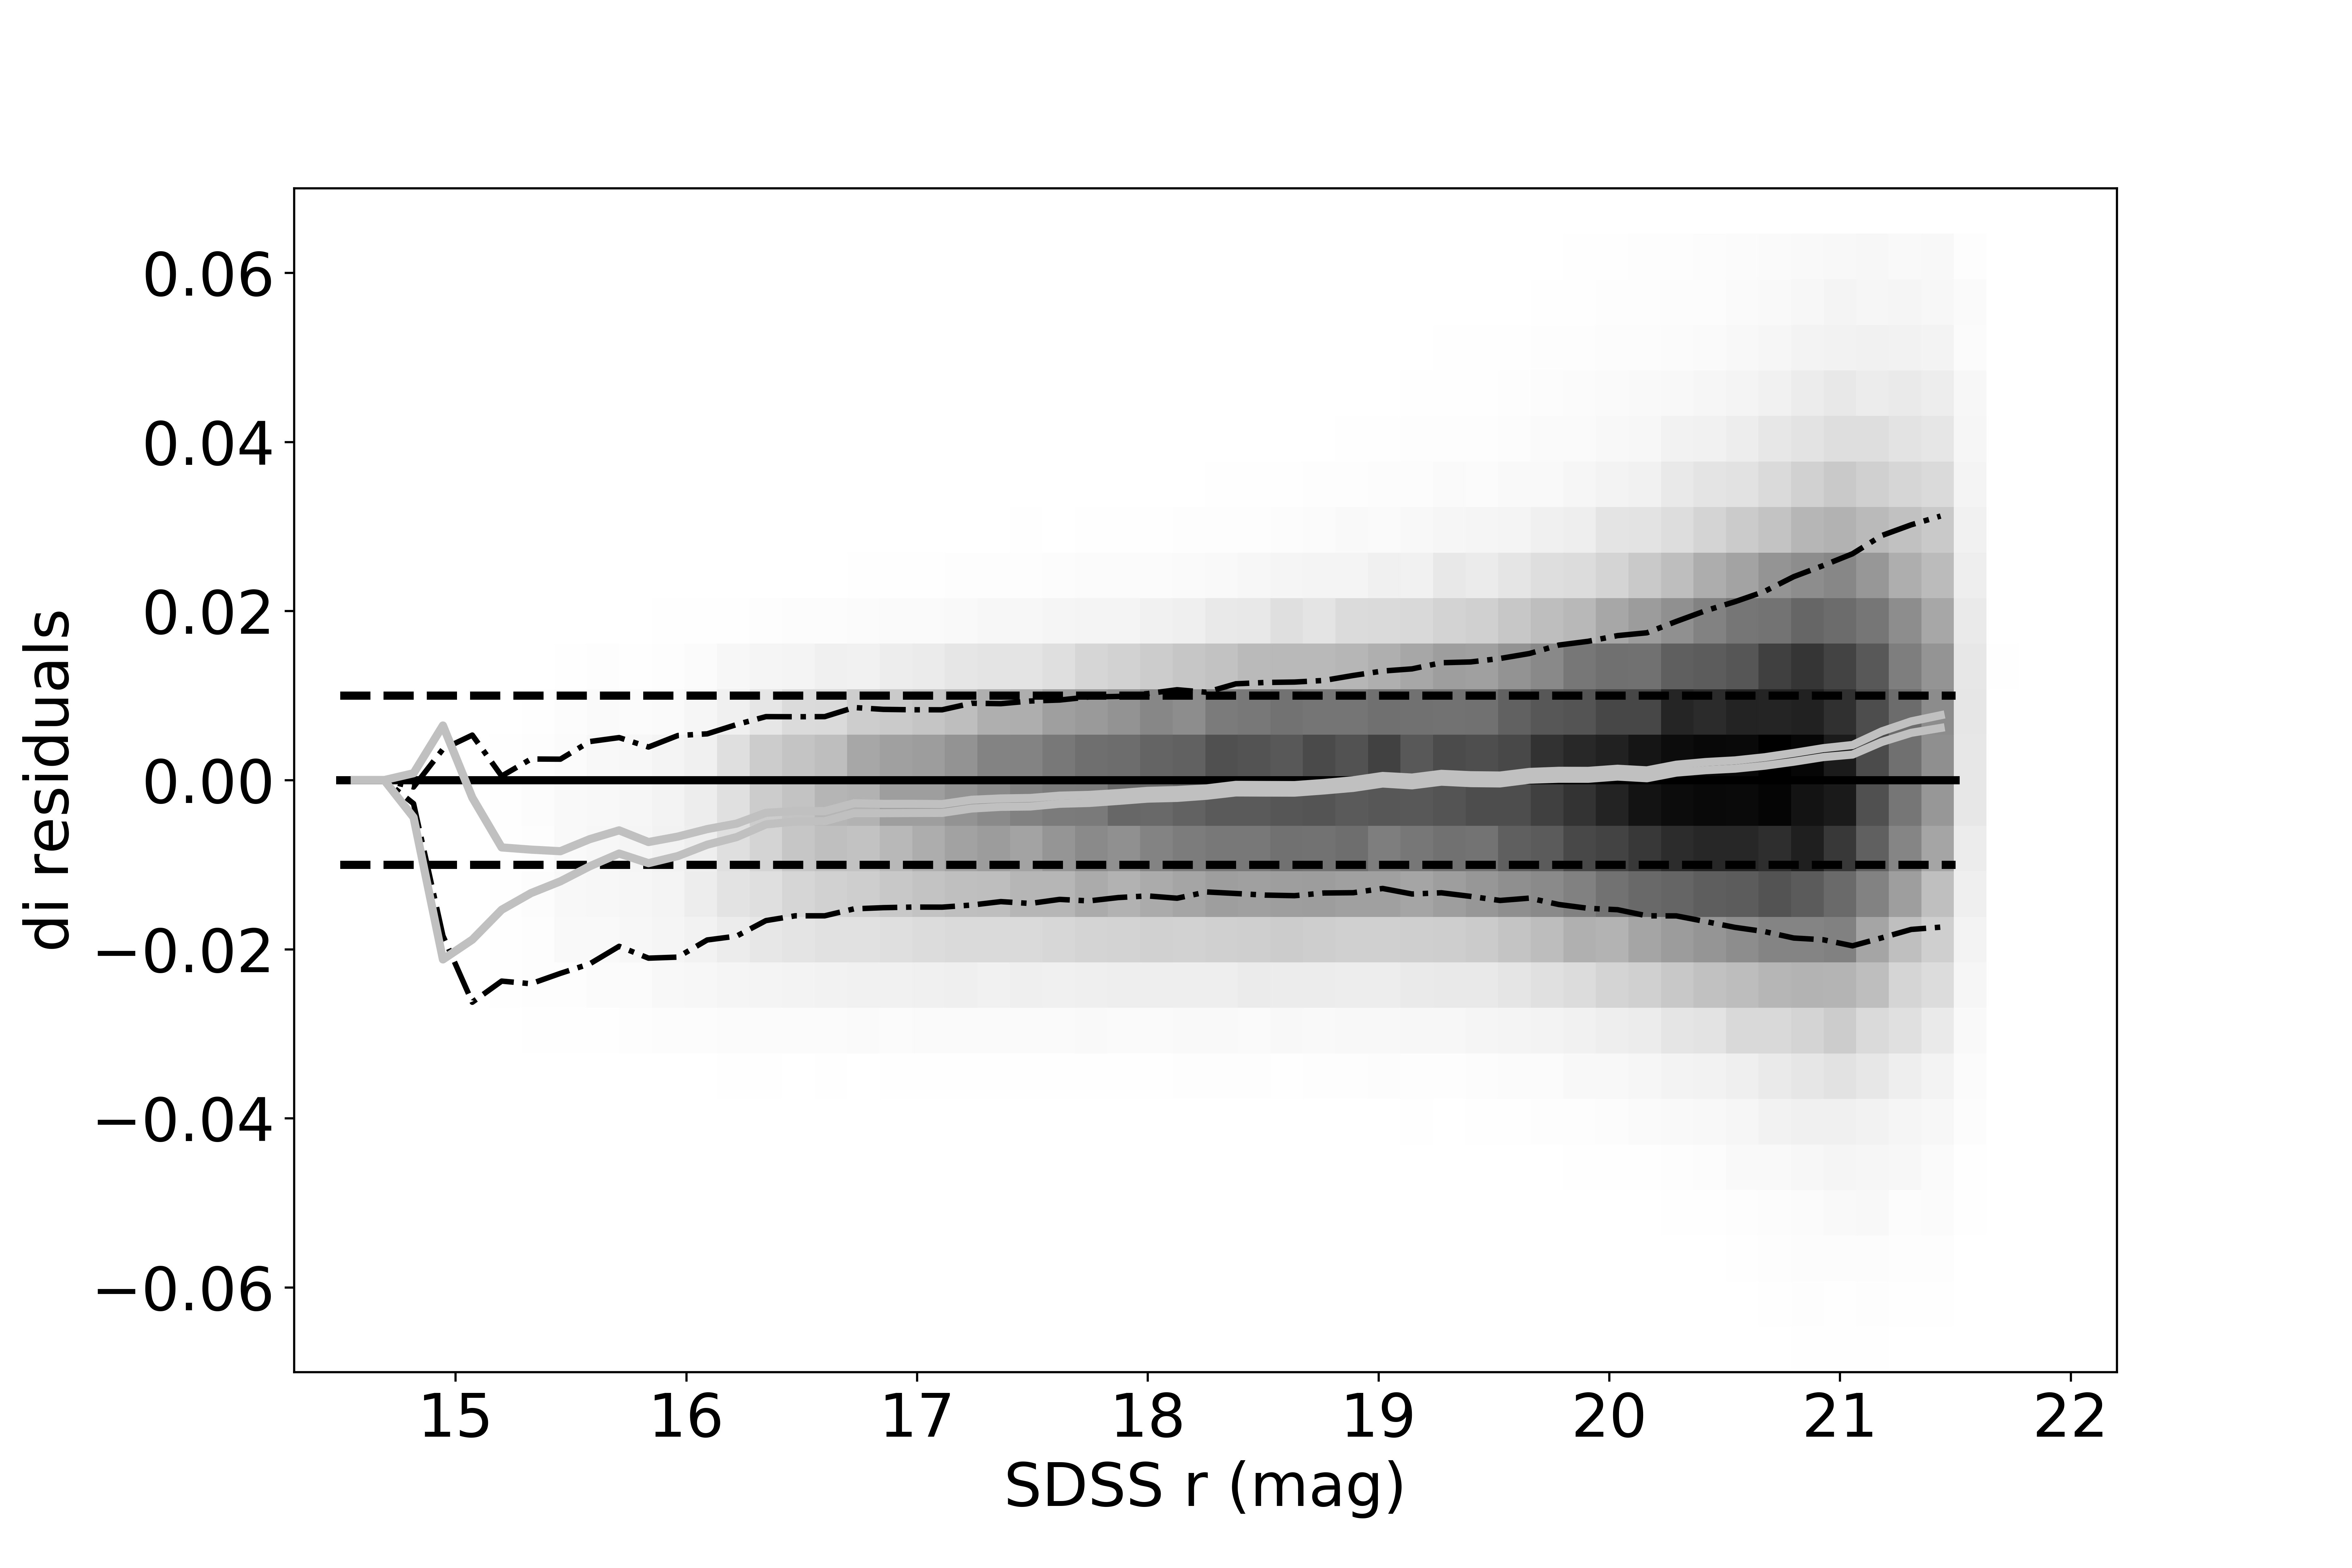
\includegraphics[width=7cm]{figures/colorResidDES2_di_rmag_Hess.png} 
\caption{A comparison of the magnitude differences between the SDSS v3.4 catalog
and DES catalog, for the $r$ and $i$ bands. Note the good agreement even at the
faint end ($20<r<21$), where Gaia Gmag magnitudes appear too faint by about
0.02 mag (see Figure~\ref{fig:gaiaJump}).} 
\label{fig:drVSr}
\end{figure}



\subsection{Comparison of the new v3.4 SDSS catalog and $u$ band data from the CFIS catalog  \label{sec:CFIStest}} 

The comparison of the new SDSS catalog with the DES and Pan-STARRS catalogs in the previous
section did not include the $u$ band. To assess the quality of $u$ band zeropoint calibration, 
we use the CFIS catalog (see Section~\ref{ssec:cfis}). The CFIS $u$ band photometry was 
calibrated using a combination of the SDSS, Pan-STARRS and GALEX UV data. Given that
we recalibrated the new SDSS catalog using Gaia data, for this comparison it shouldn't 
matter that SDSS data were used in calibration of the CFIS catalog. Nevertheless, the
results of this section should be treated with caution. 

A star-by-star comparison for about 150,000 sufficiently bright blue stars is illustrated in 
Figure~\ref{fig:CFIS}. The binned median scatter for Declination direction is 5.7 millimag with 
systematic differences of up to about 0.01 mag. The constraints in R.A. direction are more noisy, 
with residuals appearing about twice as large as in Declination direction. 
 
\begin{figure}[th!]
    \centering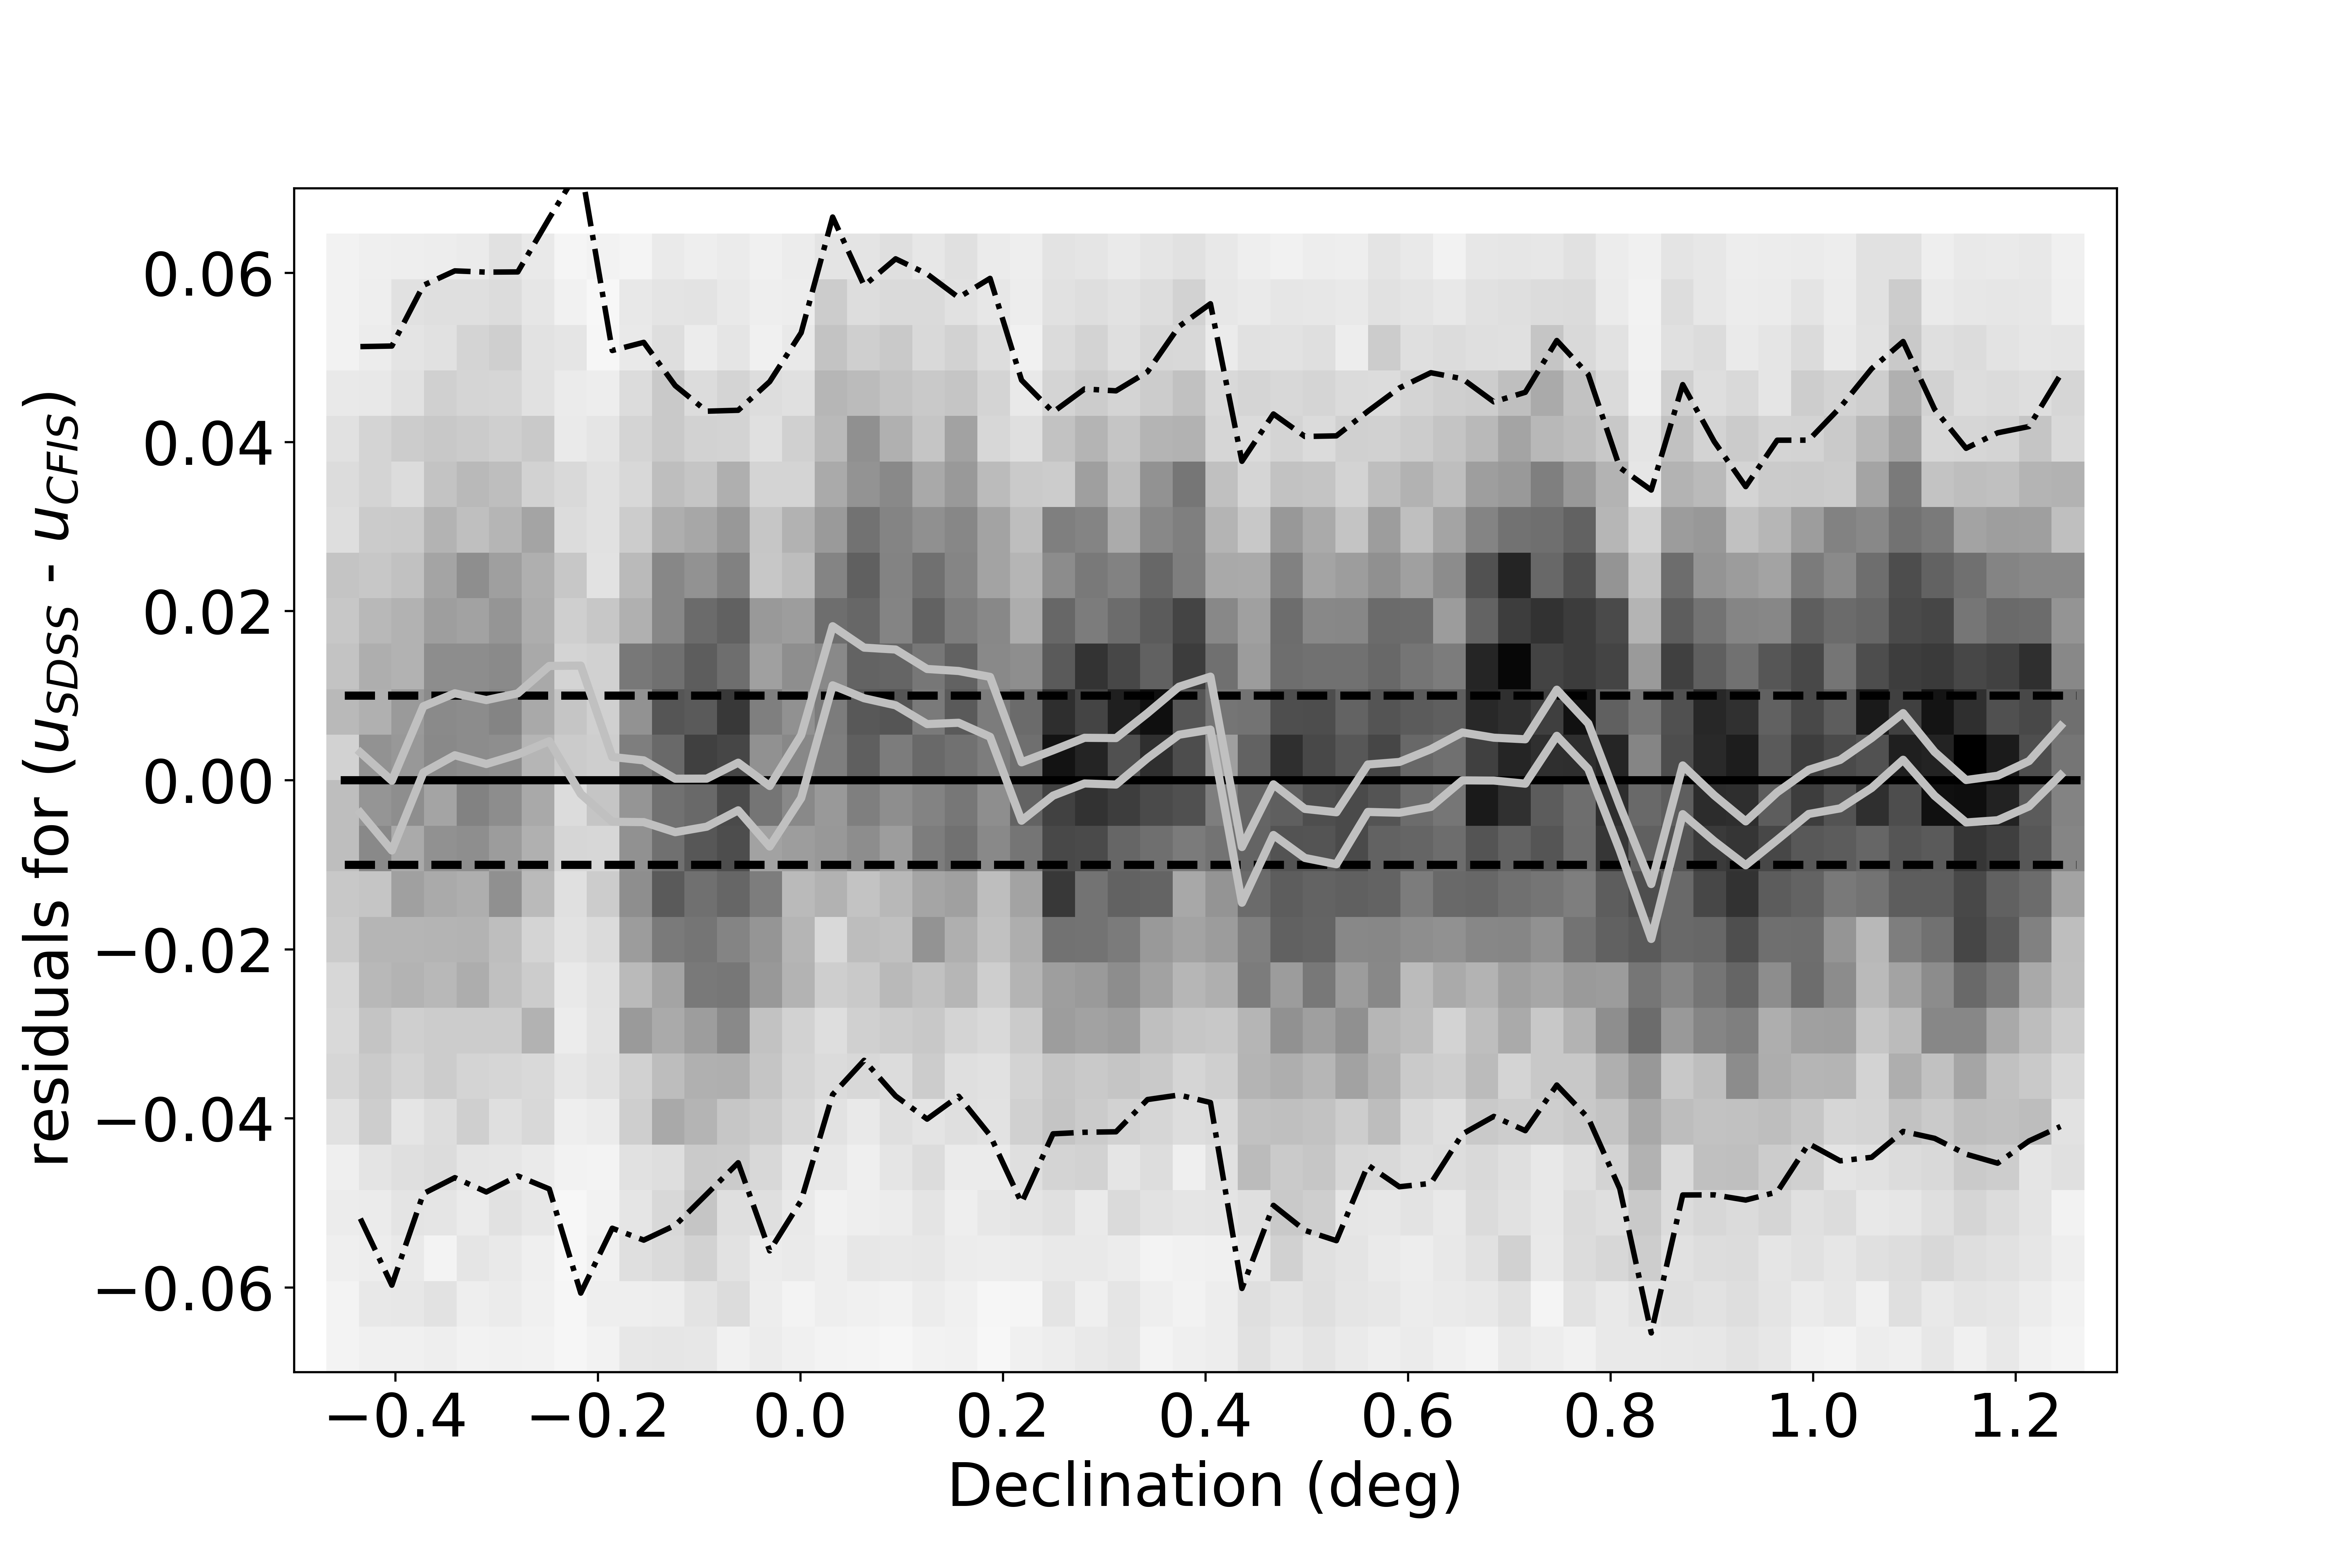
\includegraphics[width=9cm]{figures/colorResidCFISug_Dec_Hess.png} 
\caption{Analogous to Figure~\ref{fig:graycorrDec}, except that here residuals 
between the SDSS $u$ band magnitudes and $u$ band magnitudes from the CFIS
catalog (corrected for small color terms, $\sim0.05$ mag, as a function of the $u-g$ color),
for $\sim$150,000 matched stars with $1.0 <u-g < 2.1$ and $r<20$ are shown. 
The binned median scatter is 5.7 millimag. Note that the CFIS data are available
only for Declination $>$ -0.45 degree.}
\label{fig:CFIS}
\end{figure}

\subsection{Offsets from AB magnitude scale \label{sec:AB}} 




% \section{The Construction and Analysis of the New v3.4 Catalog \label{sec:v34}}


%%%% COPY BELOW TO OVERLEAF as zeljko2.tex 

We first describe the construction of the new SDSS catalog and derivation of photometric
zeropoint corrections using Gaia DR2 data, and then compare the resulting photometry to 
Gaia DR2, DES, Pan-STARRS and CFIS catalogs. 

 %%%%%%%%%%%%%%%%%%%%%%%%%%%%%%%%%%%%%%%%%

\subsection{The construction of raw SDSS catalog from light curves \label{sec:averaging}} 

Given light curve data files described in Section~\ref{ssec:DR15}, we computed the median 
and mean magnitudes, their formal uncertainties and $\chi^2$ (assuming constant brightness)
for all stars, in all five bands. Due to more observational epochs in DR15, the new data are more 
sensitive to variability; following \pO, we applied $\chi^2>3$ in the $gri$ bands, as well as  
requirements for at least 4 epochs in the same three bands and the formal uncertainty of the 
mean $r$ band magnitude below 0.05 mag. These selection criteria recovered 98.5\% stars from
the original catalog, resulting in a new catalog with 991,472 stars. 

Figure~\ref{fig:rerr_nvso} compares the numbers of epochs for matched stars and their formal
uncertainties of the mean $r$ band magnitude. The new 2020 catalog has about 2-3 times more 
measurements per star, depending on its sky position within Stripe 82. Consequently,  formal 
photometric uncertainties (``random errors'') are about 1.4-1.7 times smaller. This raw catalog
is labeled version v3.1, and is publicly available from the same
website\footnote{http://faculty.washington.edu/ivezic/sdss/catalogs/stripe82.html} 
as the original 2007 catalog. 

A star-by-star comparison of the photometry between the old and new catalogs is discussed
in Section~\ref{sec:v26v34}. 

\begin{figure}[th!]
\centering
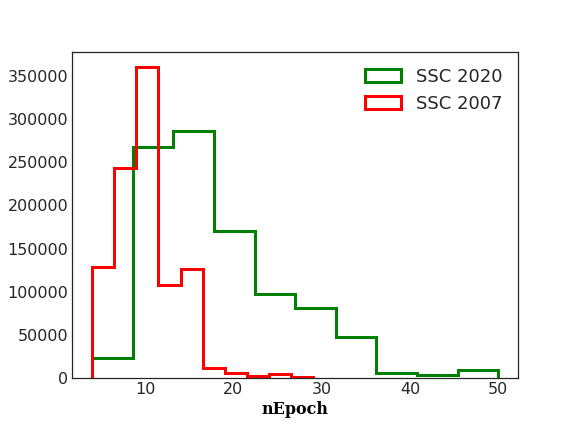
\includegraphics[width=0.4\textwidth, keepaspectratio]{figures/nepoch_compOvsN.png}
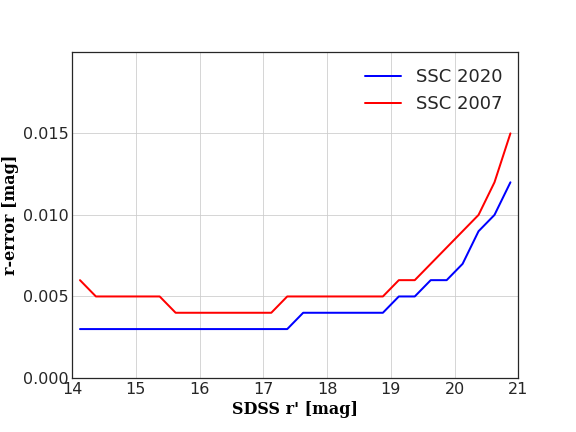
\includegraphics[width=0.4\textwidth, keepaspectratio]{figures/rerr_compOvsN.png}
\caption{{\it Left:} A comparison of the number of observational epochs for matched stars in the 2020 versus 2007 Standard Star Catalog (SSC). {\it Right:} A comparison of the median formal $r$ band photometric uncertainties of matched objects in the 2020 versus 2007 SSC, as a function of their mean $r$ magnitudes.
\label{fig:rerr_nvso}}
\end{figure}

%%%%%%%%%%%%%%%%%%%%%%%%%%%%%%%%%%%%%%%%%

\subsection{The derivation of  photometric zeropoint corrections using Gaia DR2 data\label{sec:GaiaCorr}} 

The variation of photometric zeropoints with position on the sky in the \pOc\ (see their eq.~4) was 
constrained using a combination of stellar colors \citep[the principal axes in color-color diagrams, for details 
see][]{2004AN....325..583I} and a standard star network \citep{2002AJ....123.2121S}. It is likely that 
residual errors in zeropoint calibration (e.g., a saw-tooth pattern, as a function of Declination,
was reported by \citealt{2013A&A...552A.124B}; see their Fig.~23) can be further minimized using 
uniformly calibrated space-based photometry from Gaia Data Release 2 (DR2). 

\subsubsection{Positional matching of the SDSS and Gaia catalogs}
Naively, one would positionally match the SDSS and Gaia DR2 catalogs using a matching radius of 
about 0.3 arcsec because SDSS positions are accurate to better than 0.1 arcsec per coordinate (rms) 
for sources with $r < 20.5$ mag \citep{2003AJ....125.1559P}.  However, observational epochs are
sufficiently different that stellar proper motions need to be accounted for; indeed, we find a very 
strong correlation between the SDSS-Gaia positional differences and proper motions published in 
the Gaia DR2 catalog (see the left panel in  Figure~\ref{fig:GaiaRApm}). After accounting for proper
motions,  the positions agree at the level of $\sim28$ milliarcsec (robust\footnote{We use robust estimator 
of standard deviation computed as $\sigma_G = 0.741*(q_{75}-q_{25})$, where $q_{25}$ and $q_{75}$ are 
the 25\% and 75\% quantiles, and the normalization factor 0.741 assures that $\sigma_G$ is equal to 
standard deviation for normal (Gaussian) distribution.}
rms, per coordinate). The 
residual differences are dominated by systematic errors in SDSS astrometry because there is
no increase of this rms with magnitude (see the right panel in Figure~\ref{fig:GaiaRApm}), and
because the contribution of Gaia's astrometric measurement uncertainties is negligible. 
The implied SDSS astrometric accuracy of $\sim28$ milliarcsec is substantially better than 
``$<0.1$ arcsec reported by \cite{2003AJ....125.1559P}, but note that here we used 
positions ``averaged'' over typically $\sim20$ SDSS runs (see the left panel in Figure~\ref{fig:rerr_nvso}). 

\begin{figure}[th!]
\centering 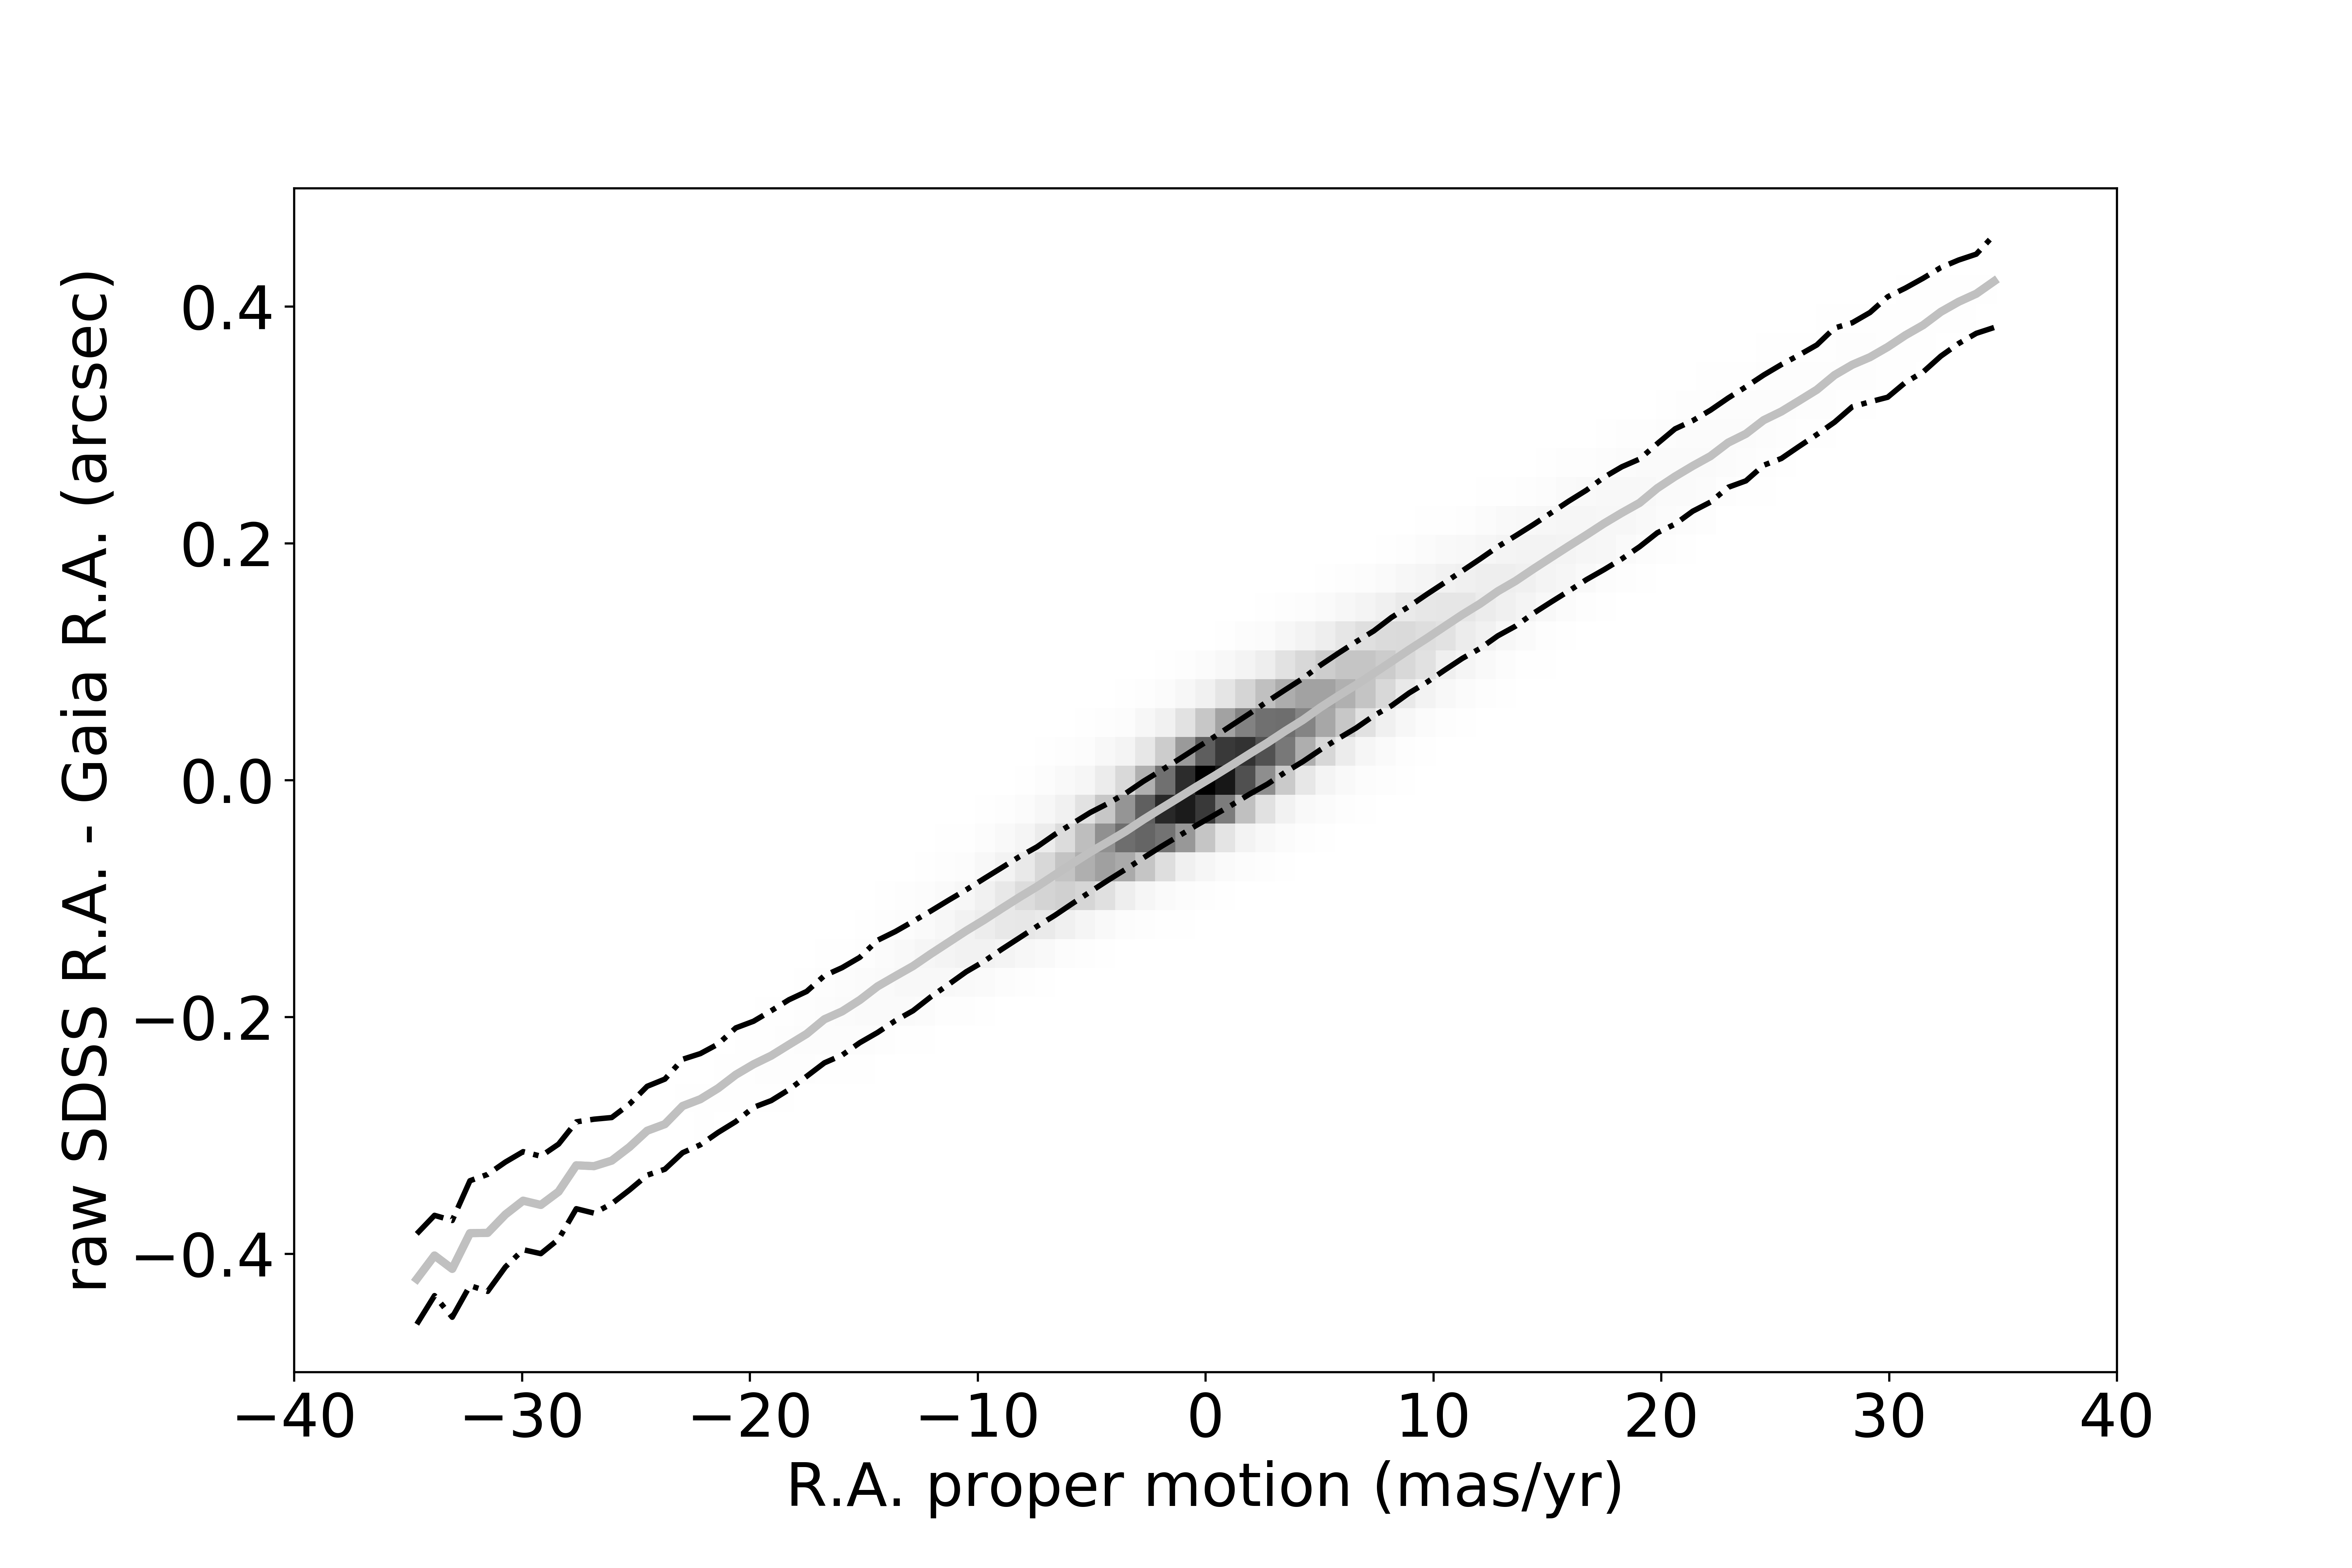
\includegraphics[width=0.4\textwidth, keepaspectratio]{figures/astroVSpm_RA_pm.png}
\centering 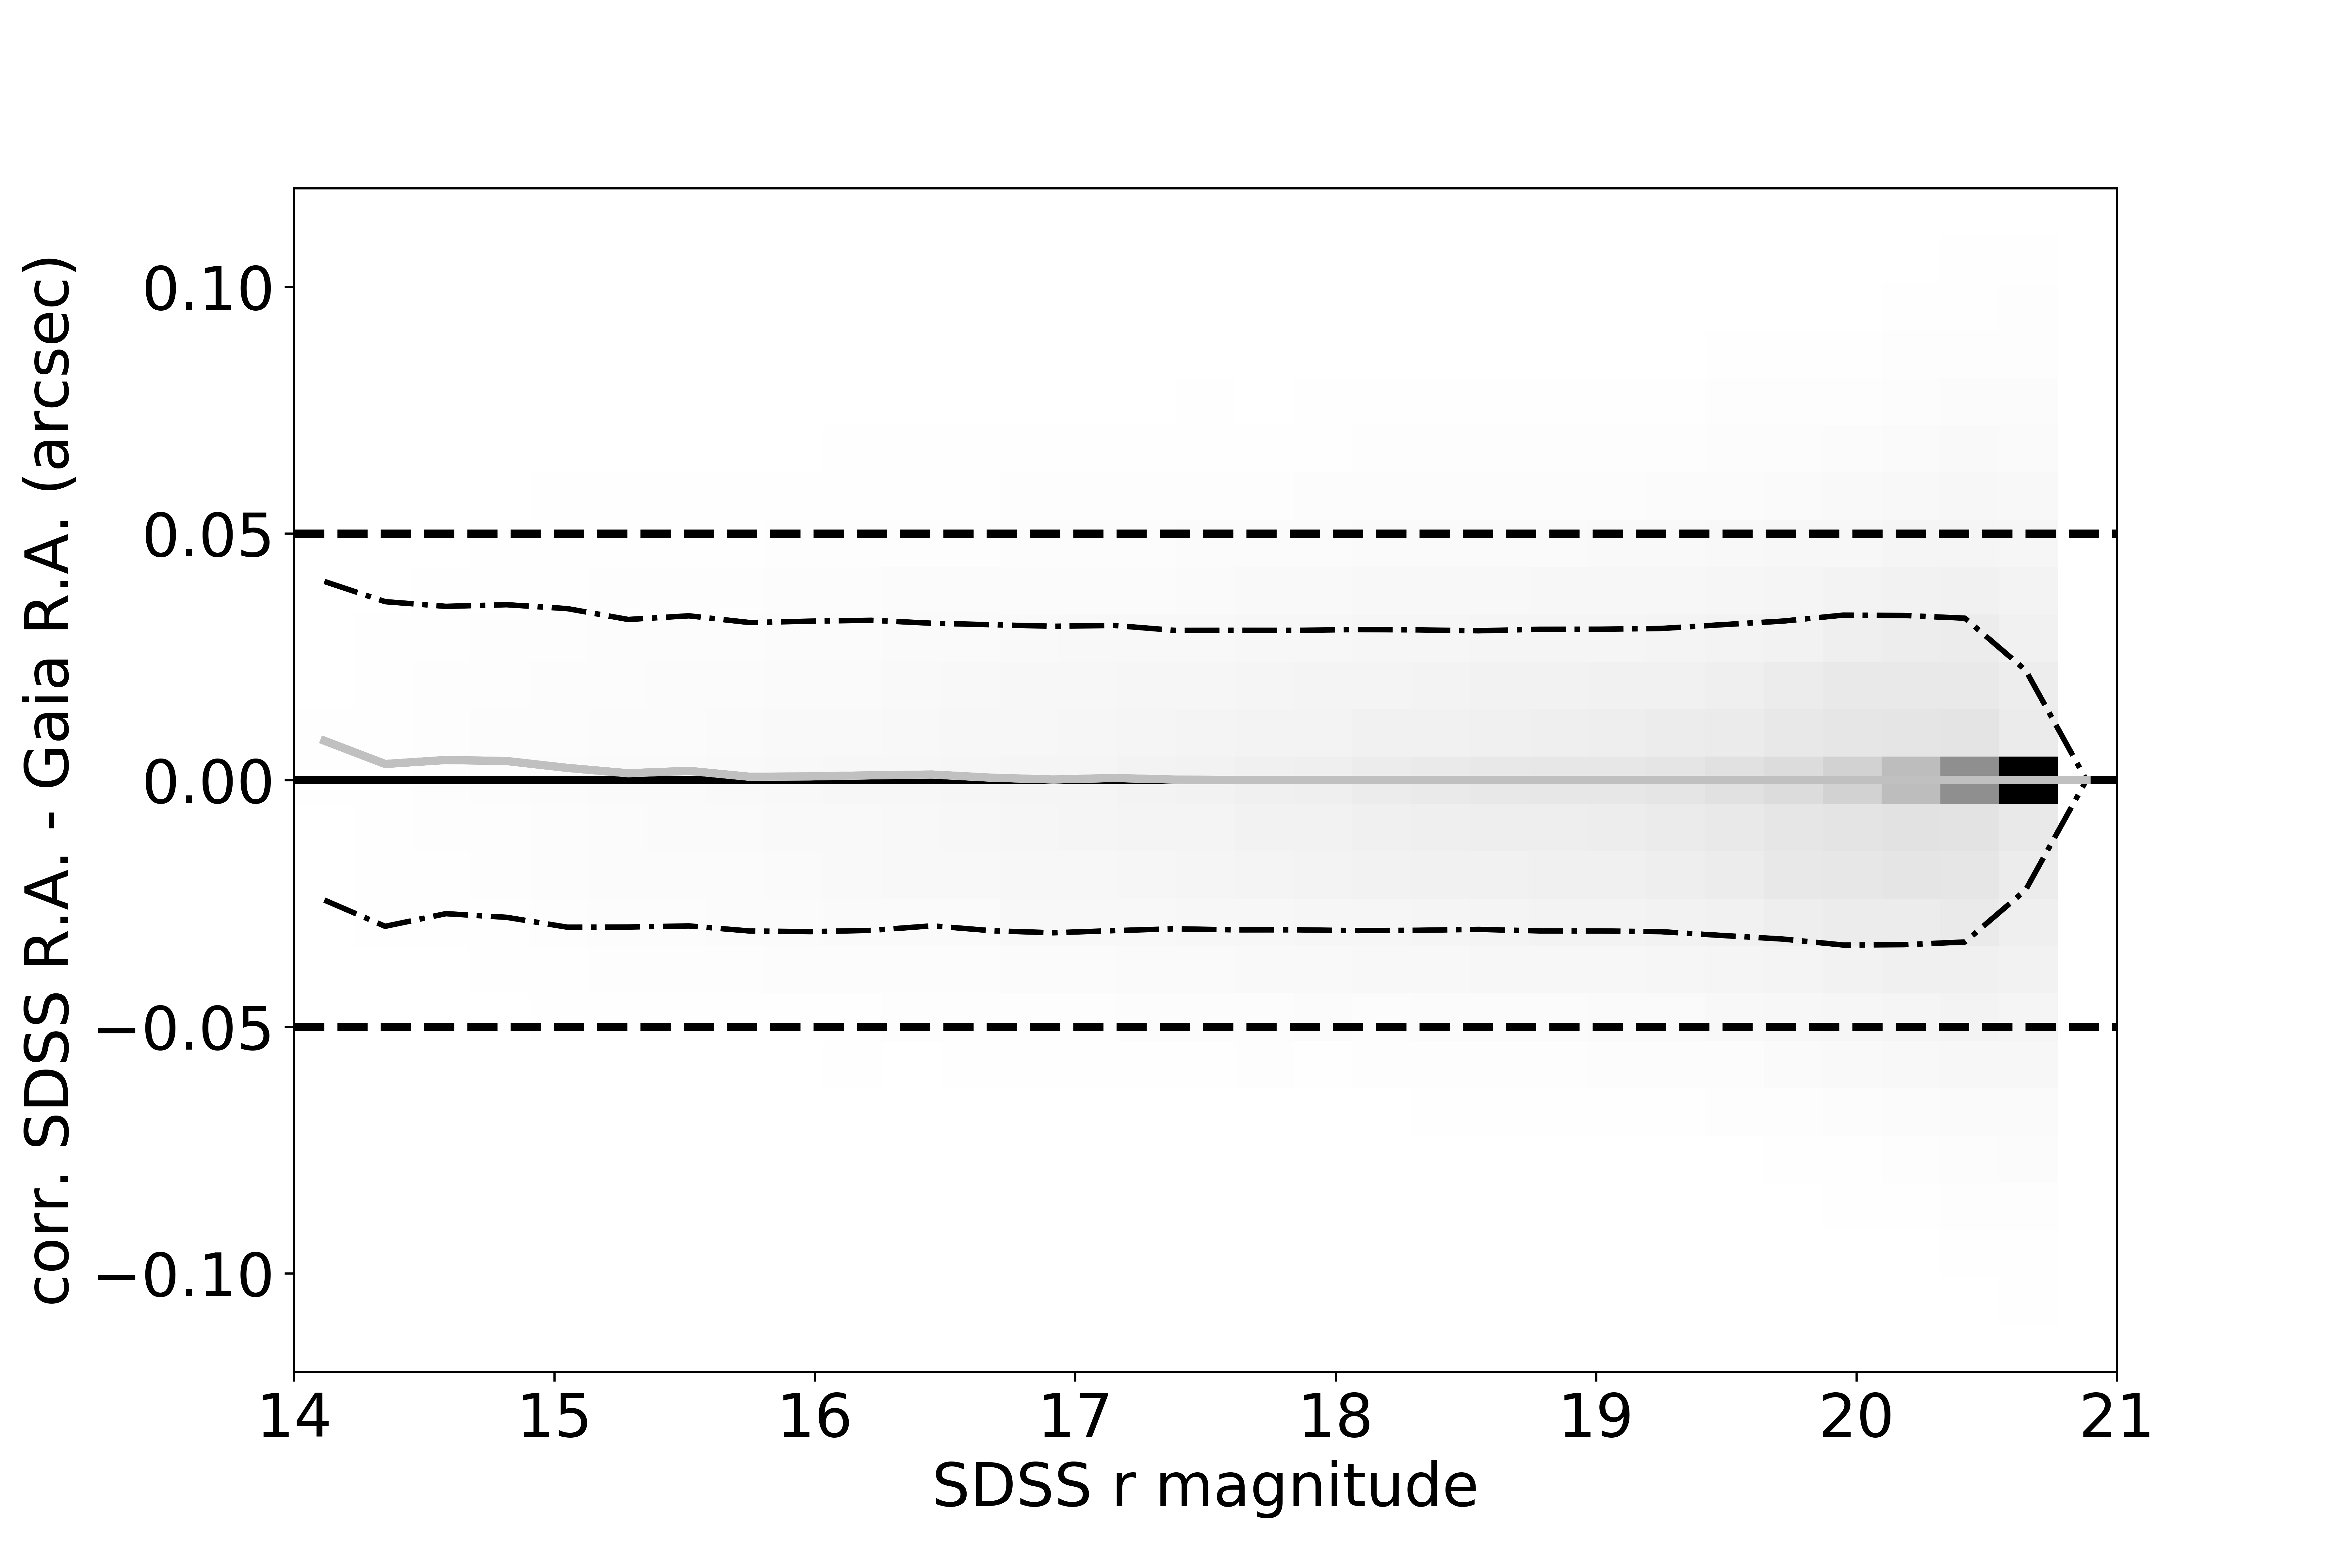
\includegraphics[width=0.4\textwidth, keepaspectratio]{figures/astroVSpm_RA_r.png}

\caption{The left panel shows the R.A. difference between SDSS and Gaia 
vs. R.A. proper motion reported by Gaia DR2. The solid line shows the median difference in bins 
of proper motion and the dashed lines mark the $\pm \sigma_G$ envelope around the medians,
where $\sigma_G$ is the robust standard deviation. The right panel shows the R.A. difference 
after correcting using the best-fit R.A. difference vs. 
proper motion curve, as a function of the SDSS $r$ magnitude. The residual differences are dominated 
by systematic errors in SDSS astrometry at the level of $\sim28$ milliarcsec (note that there is no increase with 
magnitude). Analogous plots for Declination quantities are similar. 
\label{fig:GaiaRApm}}
\end{figure}
  
%%%%%%%%%%%%%%%%%%%%%%%%%%%%%%%%%%%%%%%%%

\subsubsection{Gaia-based photometric zeropoint corrections  \label{sec:GaiaCorr2}}

Gaia DR2 reported Gmag magnitudes, which approximately span the SDSS $griz$ bandpasses, 
and BP and RP magnitudes, which approximately correspond to the blue and red halfs of the 
Gmag bandpass. We first used Gmag data to derive ``gray'' zeropoint corrections (applied to
all five SDSS bands), and then use the BP-RP color to derive zeropoint corrections for the 
$ugiz$ bands, relative to the $r$ band. 

The basic idea is simple: use Gaia's Gmag, Gmag$_{GaiaDR2}$, and the SDSS $gri$ magnitudes
to derive synthetic Gmag magnitudes based on SDSS data, Gmag$_{SDSS}$; bin the 
$\Delta$Gmag = (Gmag$_{SDSS}$-Gmag$_{GaiaDR2}$) residuals by R.A. and Dec, and 
use the median residuals per bin as the gray correction for SDSS photometry (as functions
of R.A. and Dec). Similarly, use Gaia's BP-RP color to derive synthetic $u-r$, $g-r$, $r-i$
and $r-z$ colors, and used the median residuals per bin as zeropoint corrections for 
the $ugiz$ bands. 

Given a large number of matched stars ($\sim 400,000$), and a large number of color combinations,
we do not attempt to derive analytic fits for synethtic magnitudes and colors but instead
use 0.05 mag narrow color bins and linear interpolation between the bins. We have verified
that even sixth-order polynomial fits do not provide better results than this simple 
numerical approach. An example of such a transformation is shown in Figure~\ref{fig:GrVSgi}. 


\begin{figure}[th!]
  \centering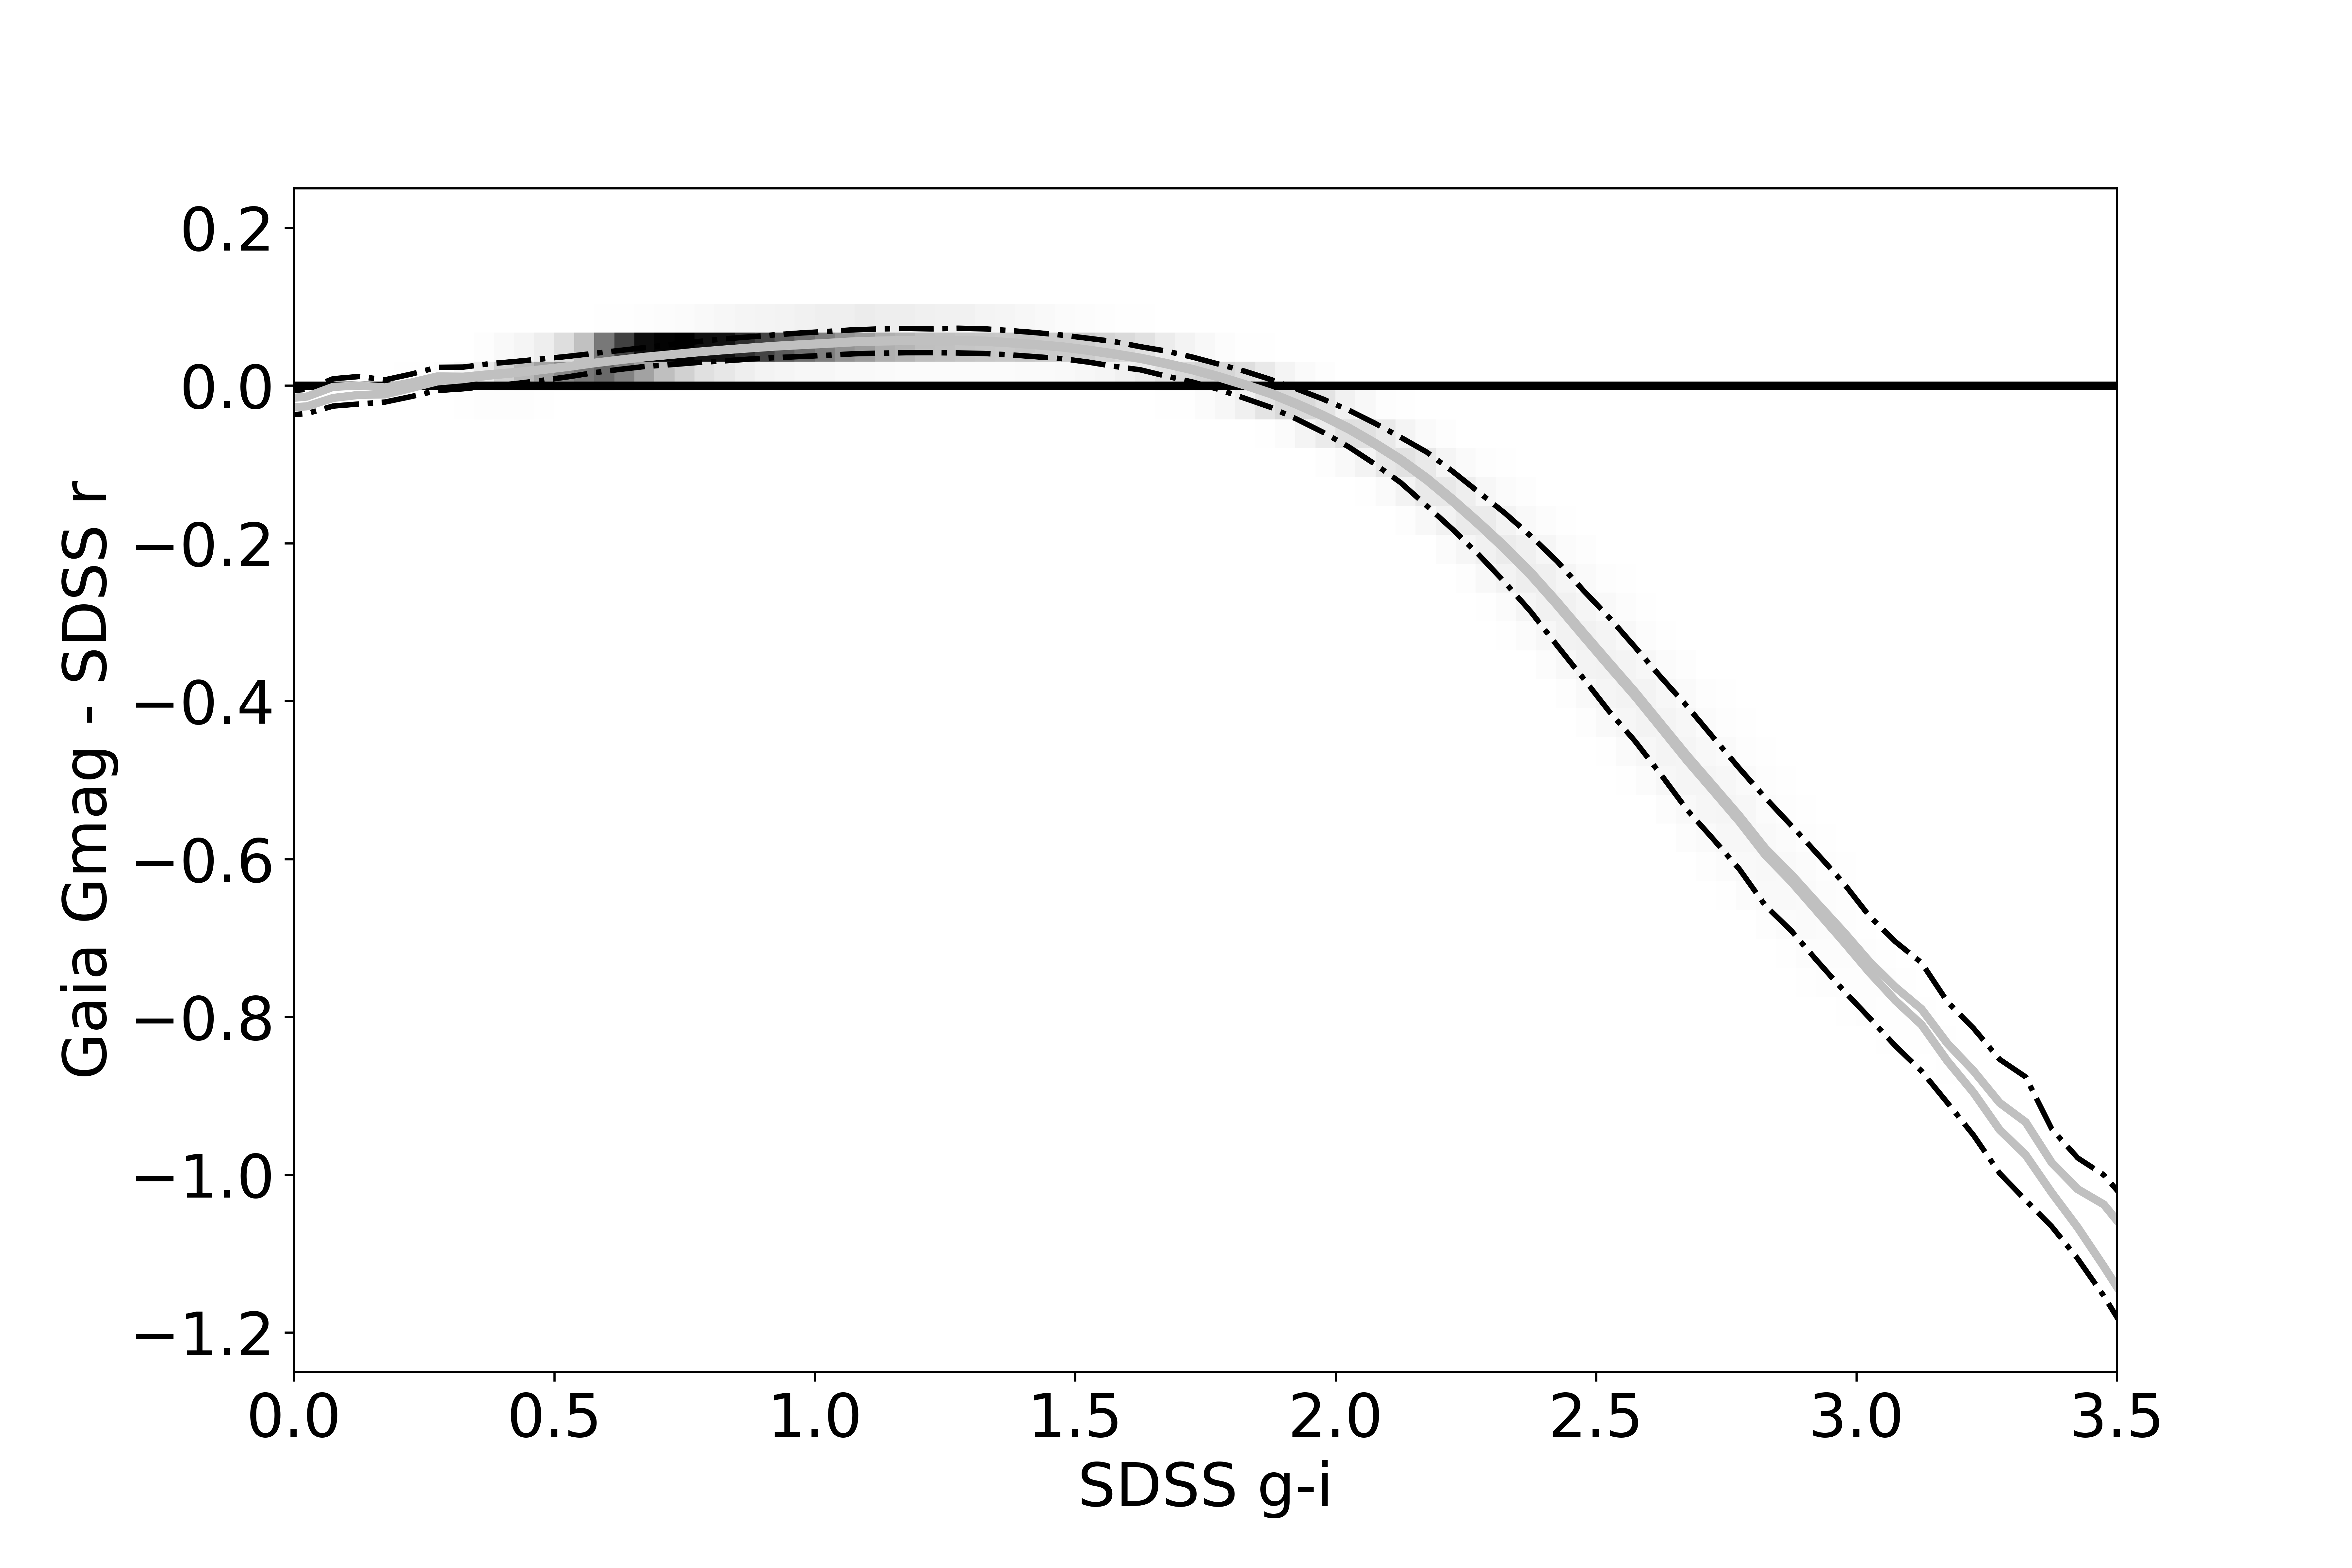
\includegraphics[width=8cm]{figures/GrVSgi.png} 
\caption{The variation of the difference between Gaia's Gmag magnitude from Data Release 2
and SDSS $r$ magnitude with the SDSS $g-i$ color.
The  color map illustrates the distribution of $\sim 393,000$ matched stars with 
$16<$Gmag$<19.5$. The two (barely distinguishable) solid lines represent the median 
values $\pm$ uncertainty of the median for 0.05 mag wide $g-i$ bins. The short-dashed 
lines show the median values $\pm$ the robust standard deviation for 
each bin. The horizontal solid line at zero is added to guide the eye. The mean of 
the two solid lines is used to derive the gray zeropoint correction, as a function of R.A.
and Declination.}
\label{fig:GrVSgi}
\end{figure}


The variation of Gmag residuals with Gmag (see Figure~\ref{fig:gaiaJump}) shows two 
interesting features. First, there is a sharp
``jump'' by about 3 millimag at Gmag$\sim$16.  This jump was a known (and 
larger problem) in Gaia Data Release 1, but appears not entirely fixed in DR2. The 
second ``feature'' is a large ($\sim0.01-0.02$ mag) discrepancy at the faint end:
about $\sim$10 millimag at Gmag=19.5 and $\sim$20 millimag at Gmag=20.5. 
A comparison of the SDSS catalog with Pan-STARRS and DES catalogs (see 
Section~\ref{sec:DESPS1} and Figure~\ref{fig:drVSr}) strongly suggests that the
origin of this discrepancy is a bias in Gaia's Gmag photometry at the faint end, rather 
than a problem with SDSS catalog (offsets between the SDSS and DES
photometry are $<1-2$ millimag at Gmag$\sim$20.5). 
 

\begin{figure}[th!]
    \centering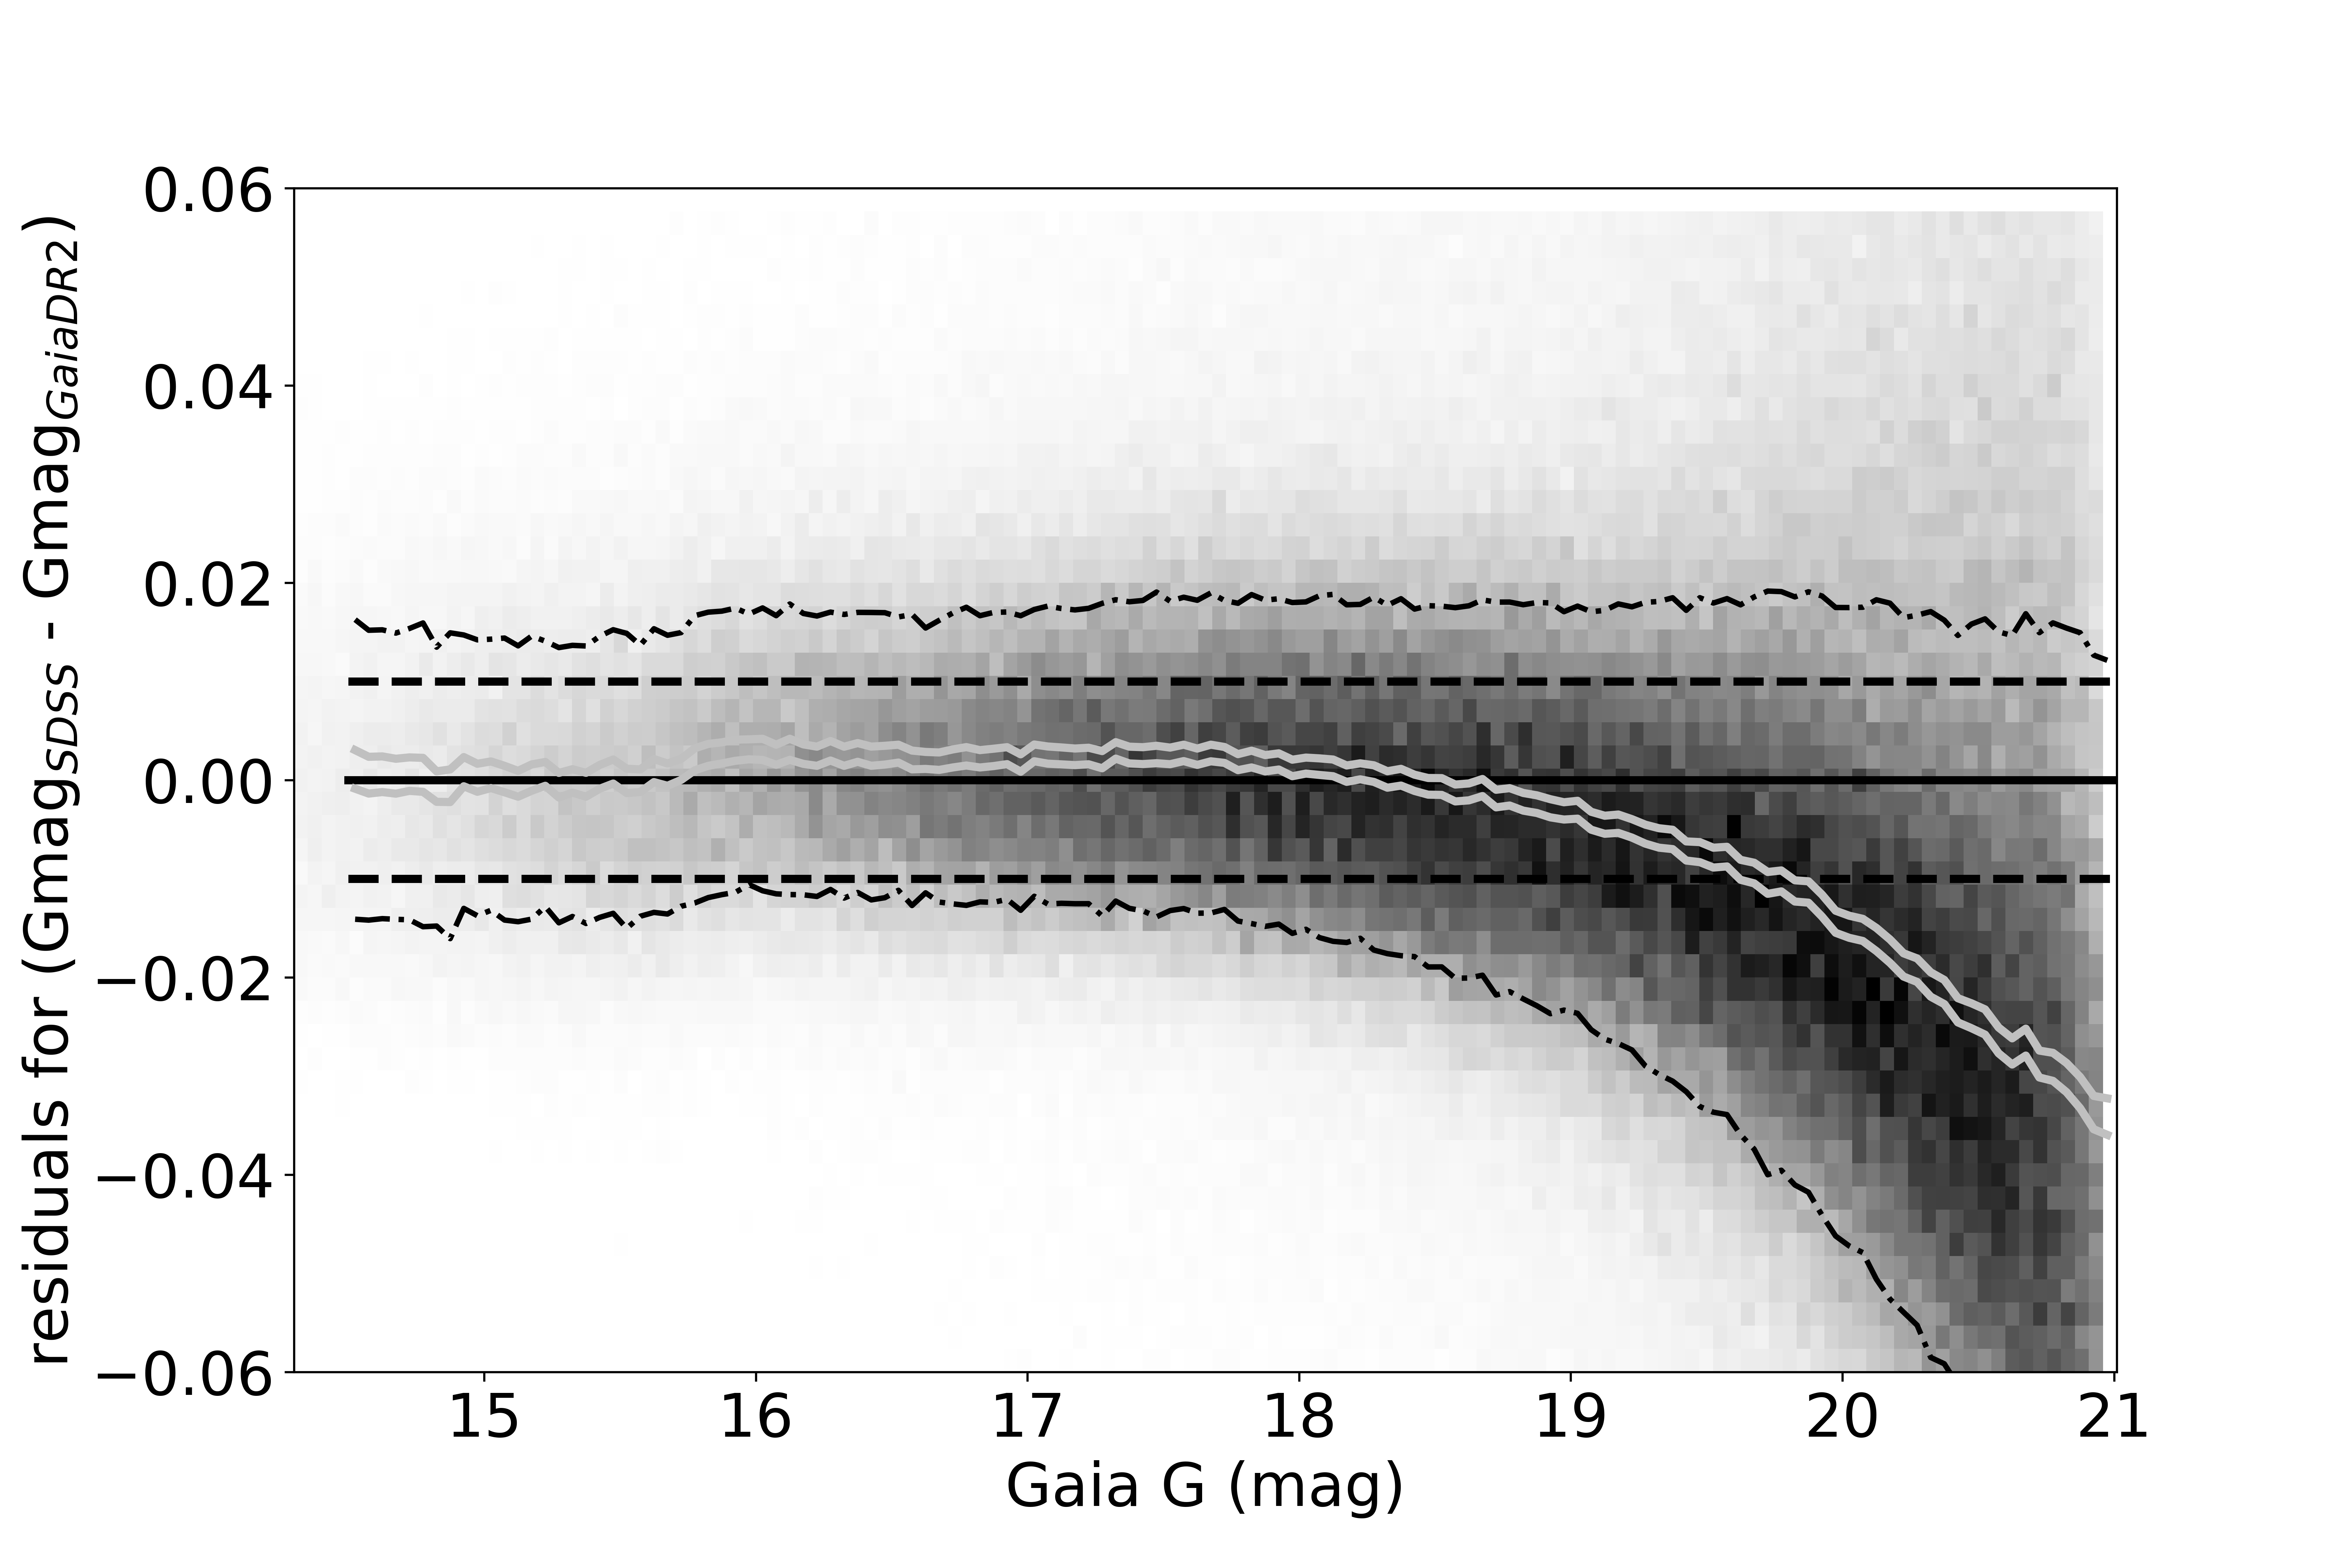
\includegraphics[width=9cm]{figures/GmagCorrectionTest_Gmag_Hess.png} 
\caption{The variation of the residuals between Gaia's Gmag from Data Release 2
and synthetic Gmag values generated using SDSS $gri$ photometry. The two solid 
lines represent the median values $\pm$ uncertainty of the median for each
0.05 mag wide Gmag bin. The short-dashed lines show the median values $\pm$ 
the robust standard deviation for each bin. The horizontal solid and long-dashed 
lines at zero and $\pm$0.01 mag, respectively, are added to guide the eye.
Note the jump by about 3 millimag at Gmag$\sim$16 -- this jump was a known and 
larger problem in Gaia Data Release 1, and apparently not entirely fixed in DR2. 
Note also large ($\sim0.01-0.02$ mag) discrepancy at the faint end -- a comparison 
of the SDSS catalog with Pan-STARRS and DES catalogs (see Figure~\ref{fig:drVSr}) 
suggests that its origin is a bias in Gaia's photometry at the faint end, rather than 
a problem with SDSS photometry.}
\label{fig:gaiaJump}
\end{figure}


Given these two features, we limit the calibration sample to the $16<$Gmag$<19.5$
magnitude range. We further restrict calibration stars to the $0.4 < g-i < 3.0$ color 
range (approximately A0 to M5 spectral range), yielding a sample of $\sim372,000$ stars. 
The behavior of median Gmag residuals per R.A. and Declination bin is shown in 
Figures~\ref{fig:graycorrRA} and \ref{fig:graycorrDec}. 


\begin{figure}[th!]
  \centering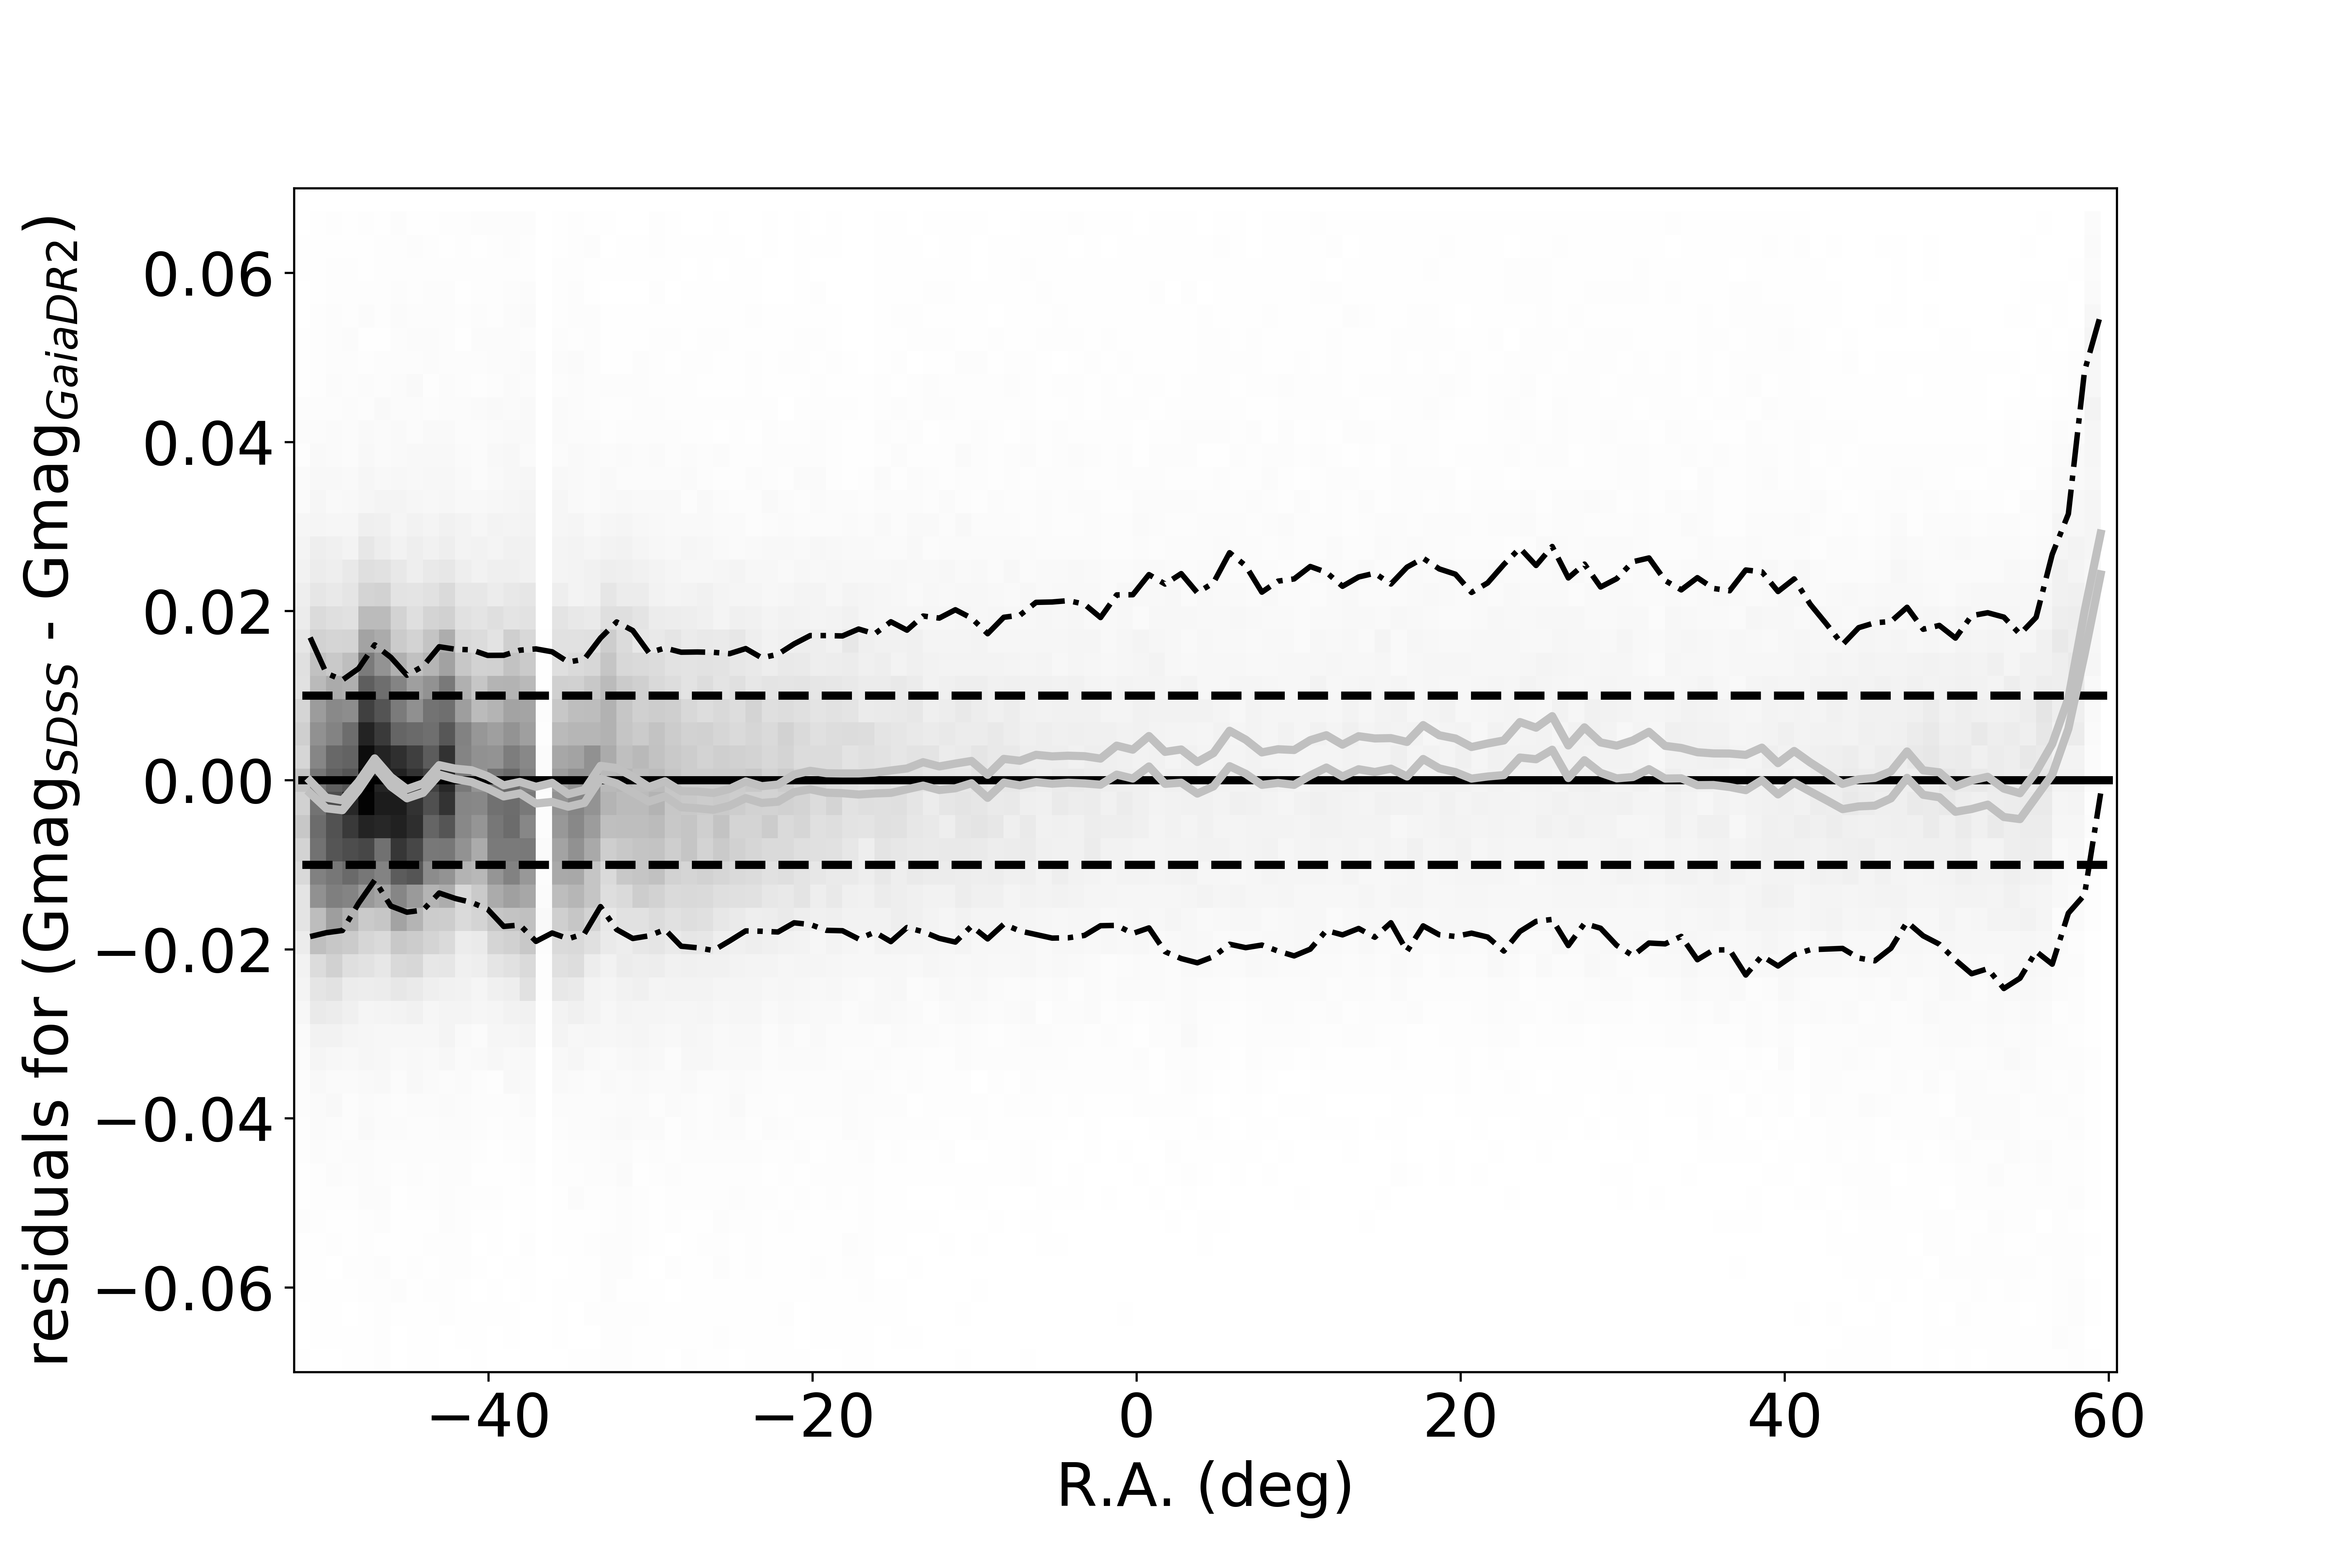
\includegraphics[width=8cm]{figures/GmagCorrection_RA_Hess.png} 
\caption{The R.A. variation of the residuals between Gaia's Gmag from DR2
and synthetic Gmag values generated using SDSS $gri$ photometry. The 
color map illustrates the distribution of $\sim 372,000$ matched stars with 
$16<$Gmag$<19.5$ and $0.4 < g-i < 3.0$. The two solid lines represent the 
median values $\pm$ uncertainty of the median for 1 degree wide R.A. bins. 
The short-dashed lines show the median values $\pm$ the robust standard 
deviation for each bin. The horizontal solid and long-dashed lines at zero and 
$\pm$0.01 mag, respectively, are added to guide the eye. The mean of the two 
solid lines is the gray correction, as a function of R.A., applied to the SDSS 
$ugriz$ magnitudes. The standard deviation for the applied correction is 3.5 millimag.}
\label{fig:graycorrRA}
\end{figure}

\begin{figure}[th!]
    \centering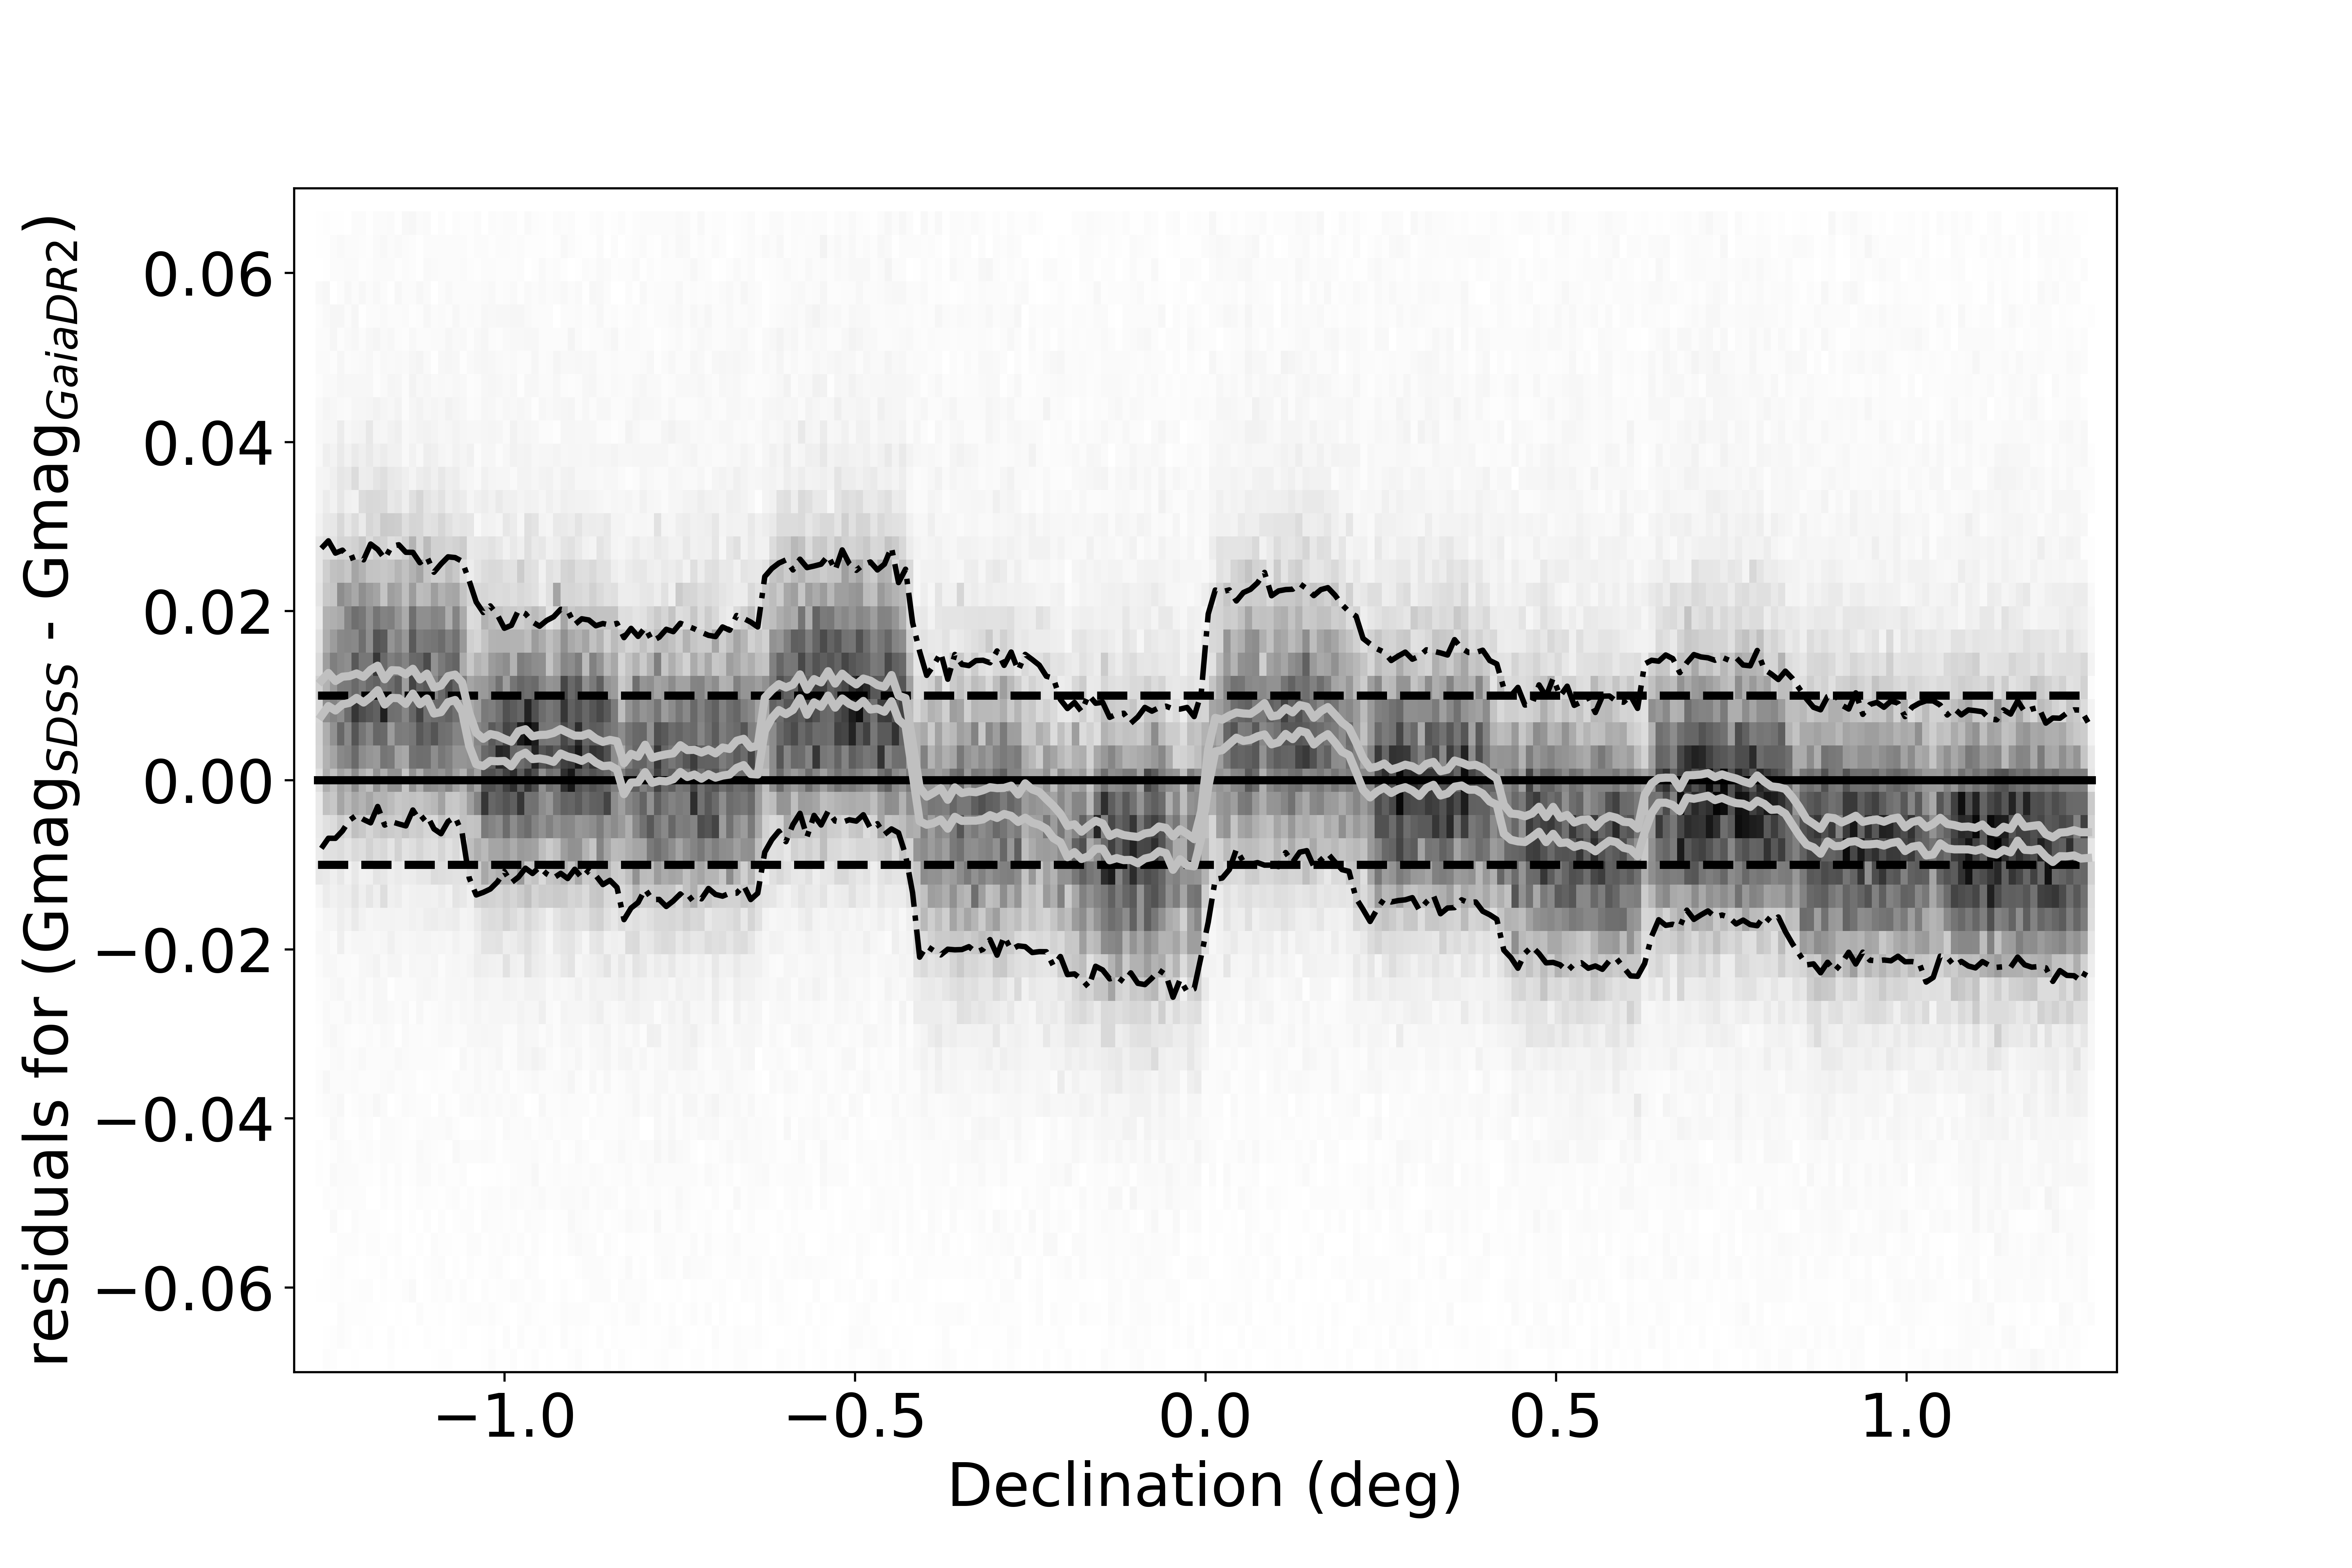
\includegraphics[width=9cm]{figures/GmagCorrection_Dec_Hess.png} 
\caption{Analogous to Figure~\ref{fig:graycorrRA}, except that here results are shown for
0.01 degree wide Declination bins. The 12 clearly visible regions correspond to
two SDSS scans (in R.A. direction) and six CCD columns in the SDSS camera. 
The standard deviation for the applied correction is 6.2 millimag, with a maximum
absolute value of $\sim0.01$ mag.}
\label{fig:graycorrDec}
\end{figure}


Except for a few degrees long region at the edge of Stripe 82 (R.A.$>$55 deg), the
SDSS photometric zeropoints are remarkably stable with respect to R.A.; the scatter
is only 3.5 millimag. On the other hand, there are clear deviations in Declination 
direction, which clearly map to the 12 scanning strips that fill Stripe 82. We note
that discrepancies never exceed 0.01 mag (with a scatter of 6.2 millimag), which was 
the claimed accuracy of the \pOc. Thanks to a large number of stars in the sample,
and well calibrated Gaia's photometric zeropoints across the sky, we can now 
constrain SDSS zeropoints with a precision of about 1 millimag per 0.01 degree
wide Declination bin. 

The residuals shown in Figures~\ref{fig:graycorrRA} and \ref{fig:graycorrDec} are
applied as ``gray'' zeropoint corrections to $ugriz$ magnitudes, as functions of 
R.A. and Declination, to all 991,472 stars in the catalog. This catalog version was
labeled v3.1, and it is publicly available\footnote{See http://faculty.washington.edu/ivezic/sdss/catalogs/stripe82.html}. 

In the next re-calibration step, we derive synthetic $u-r$, $g-r$, $r-i$ and $r-z$ colors
from Gaia's BP-RP color, using the same binning procedure as we used above for 
Gmag$-r$ vs. $g-i$ variation (see Figure~\ref{fig:GrVSgi}). An example of color residuals 
is shown in Figure~\ref{fig:riresid}.  The median residuals per R.A. and Declination bins 
are then used as zeropoint corrections for the $ugiz$ bands. We required that the median
offsets for all stars are vanishing and thus photometry in the new catalog is on the 
same AB scale as the old catalog (for related discussion, see Section~\ref{sec:AB}). 
The robust standard deviation for all zeropoint corrections is listed in Table~\ref{tab:GaiaRMS}. 

\begin{deluxetable}{l|c|c}[ht!]
\tablecaption{The robust standard deviation for binned SDSS-based vs. Gaia-based color residuals$^a$. \label{tab:GaiaRMS}}
\tablehead{
\colhead{Color } & \colhead{rms for R.A.} & \colhead{rms for Dec}
}
\startdata
 gray (Gmag) &    3.5         &    6.2   \\
    $u-r$        &   0.0$^b$  &   20.4   \\     
    $g-r$        &   4.0         &    4.2    \\
    $r-i$         &   4.1         &    3.2    \\ 
    $r-z$        &   7.4         &    2.9    \\ 
\enddata
\tablenotetext{a}{The standard deviation for applied Gaia-based zeropoint corrections. The robust standard deviation 
is estimated using interquartile range. The units are millimag.} 
\tablenotetext{b}{For the $u$ band, we could not confirm the R.A. behavior of Gaia-based zeropoint correction 
with the CFIS data and didn't apply it. The large $u$ band correction as a function of Declination was validated 
with the CFIS data (see Section~\ref{sec:CFIStest}).} 
\end{deluxetable}
 

\begin{figure}[th!]
    \centering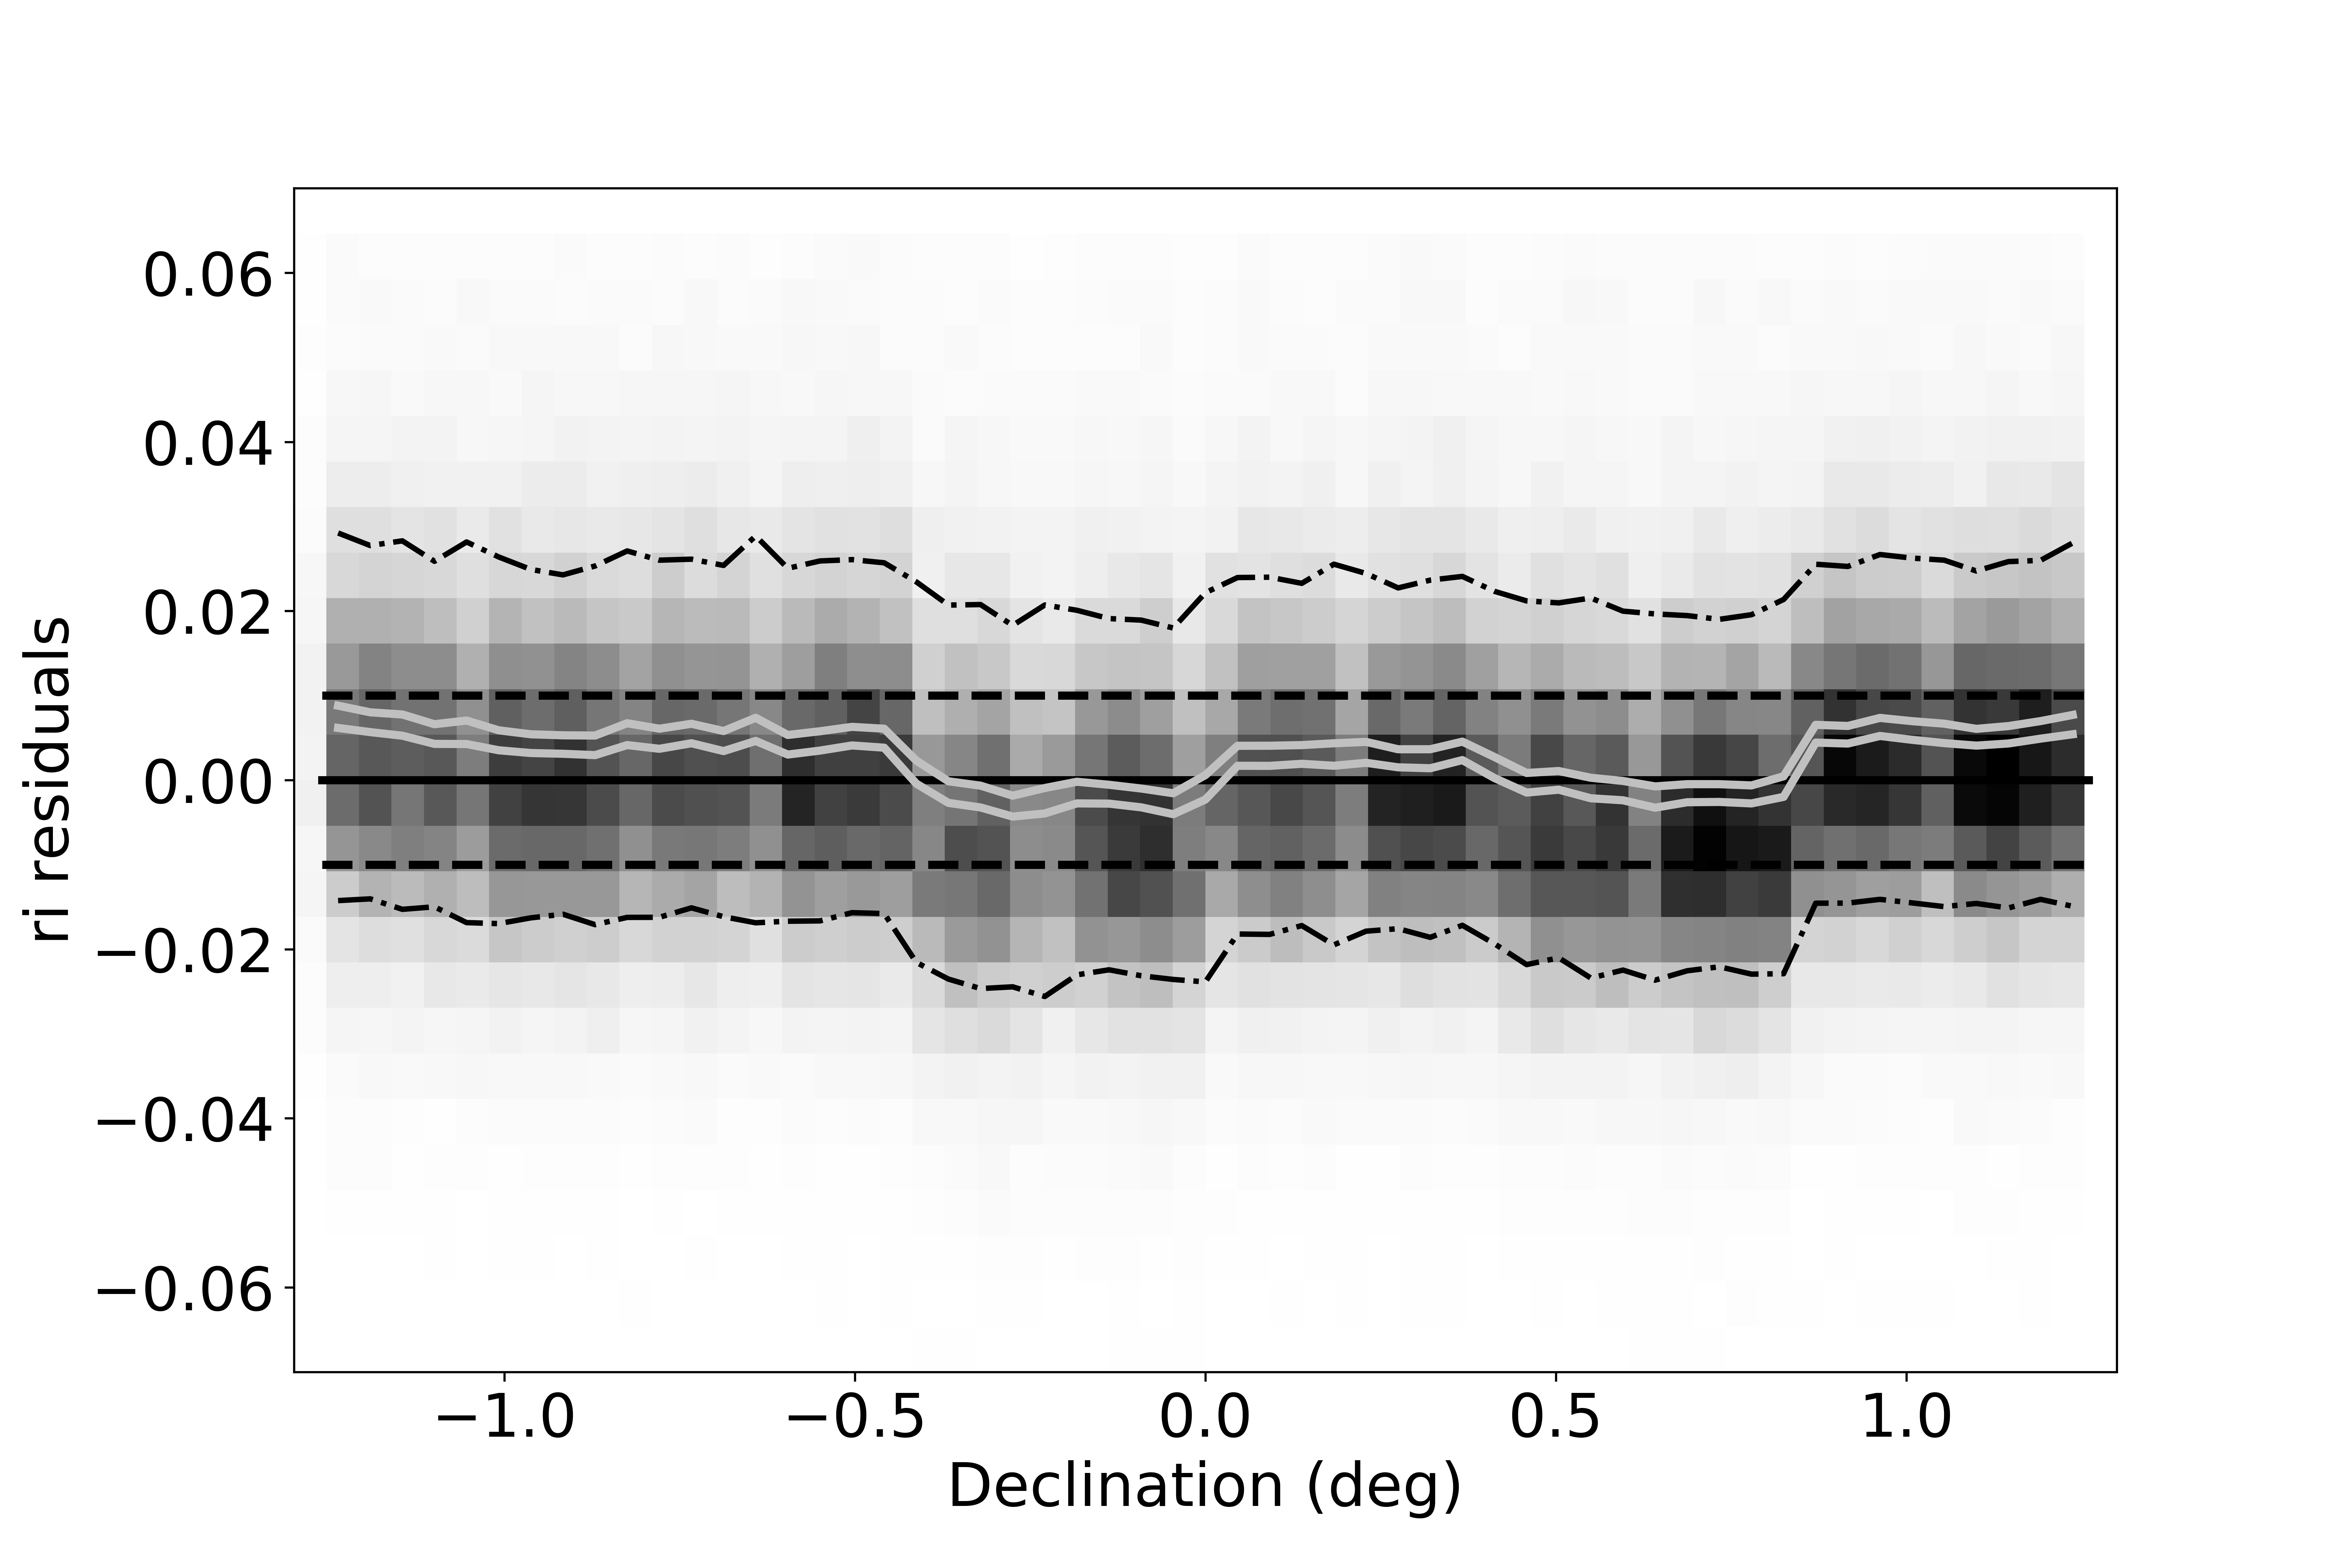
\includegraphics[width=9cm]{figures/colorResidGaiaColorsB_ri_Dec_Hess.png} 
\caption{Analogous to Figure~\ref{fig:graycorrDec}, except that here residuals 
correspond to differences between the SDSS $r-i$ color and a synthetic $r-i$ color
generated using Gaia's $BP-RP$ color. Note the signature of SDSS camera columns
at the level of a few millimags. The standard deviation for the binned medians is 
3.2 millimag (for other bands, please see Table~\ref{tab:GaiaRMS}.}
\label{fig:riresid}
\end{figure}


The largest corrections were derived for the $u$ band. Given that Gaia's BP-RP
color does not strongly constrain the $u$ band flux, we used the CFIS catalog 
(see Section~\ref{ssec:cfis}) as an independent verification test. We verified that
zeropoint errors in the SDSS catalog implied by Gaia's and CFIS data agree at the
level a few millimags in Declination direction, but found $\sim$0.01-0.02 mag
large inconsistencies for R.A. bins. For this reason, we only applied $u$ band 
correction in Declination direction. The plausible $u$ band zeropoint errors in 
the new catalog are further discussed in Section~\ref{sec:CFIStest}. This final 
catalog version was labeled v3.4, and it is also publicly available. 

 %%%%%%%%%%%%%%%%%%%%%%%%%%%%%%%%%%%%%%%%%


\subsubsection{Validation of recalibration  \label{sec:SSCvsGaia}} 
  
By construction, the new v3.4 catalog should not show appreciable zeropoint residuals when 
binned by R.A. and Declination. We have verified this expectation for all colors used in 
recalibration. For illustration, Figure~\ref{fig:grVSgaiaRADec} shows such a test for the $g-r$ 
color, with binned median scatter of the order 1 millimag. 

\begin{figure}[th!]
    \centering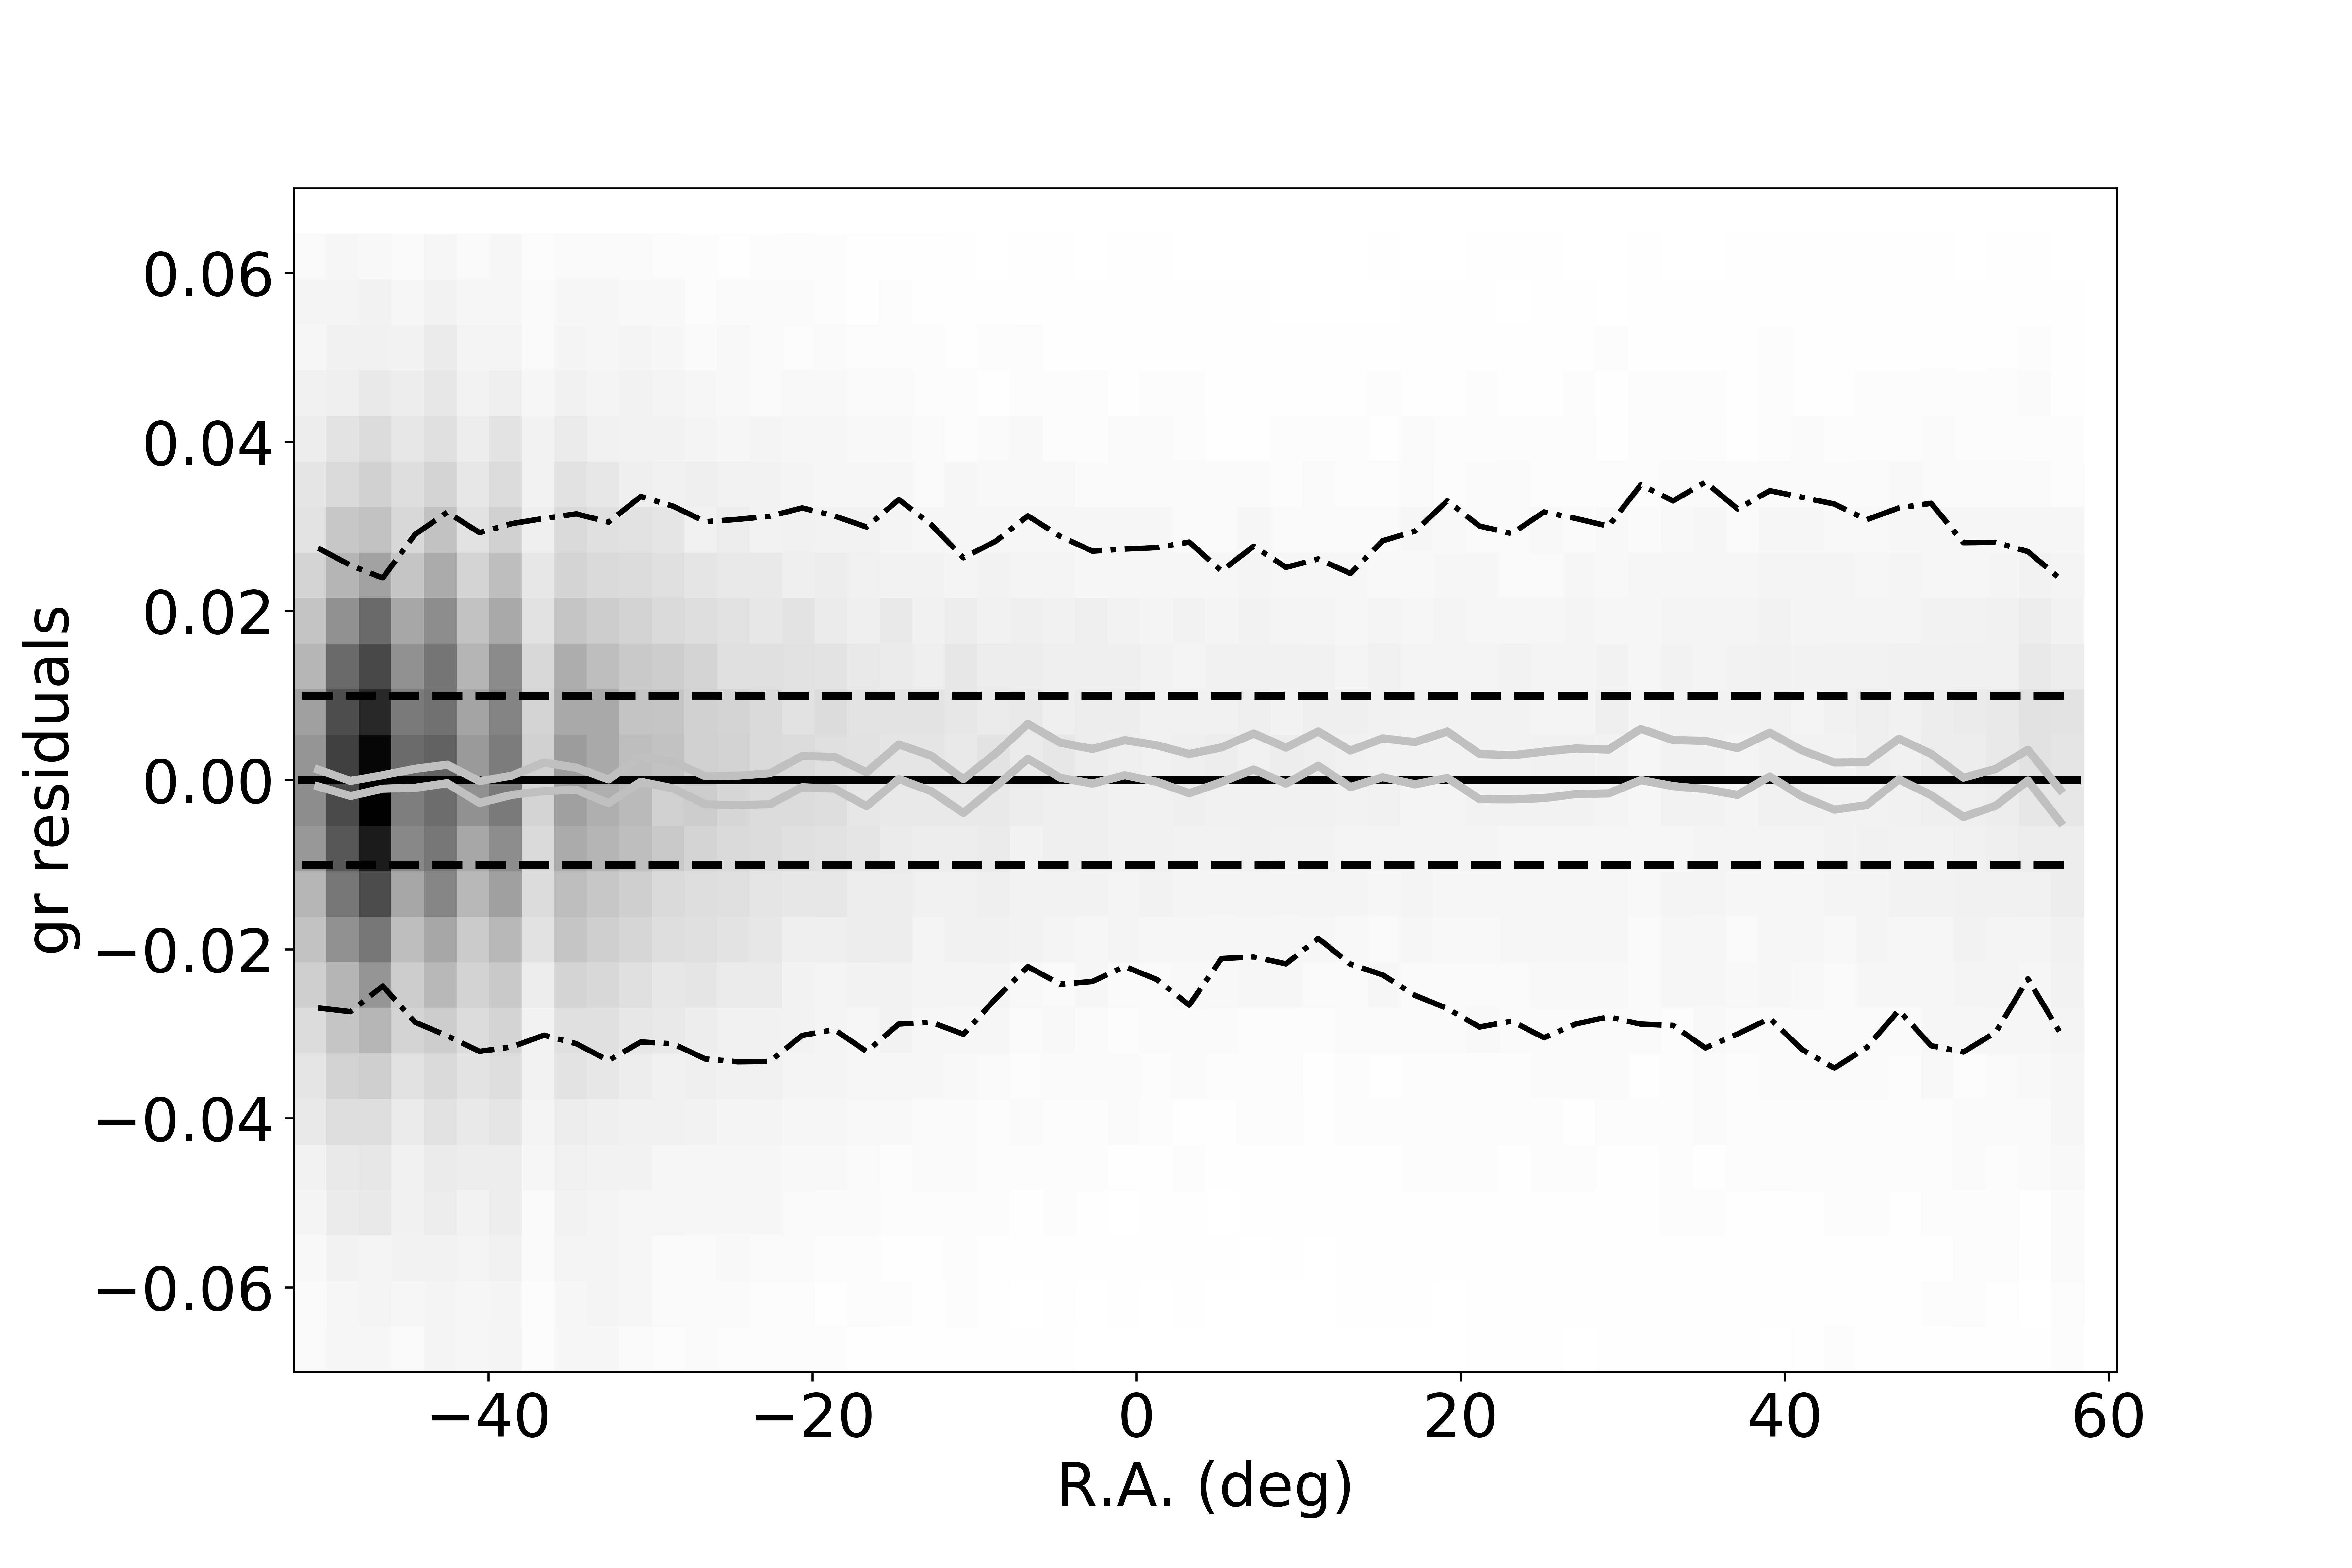
\includegraphics[width=7cm]{figures/colorResidGaiaColors_gr_RA_Hess.png} 
    \centering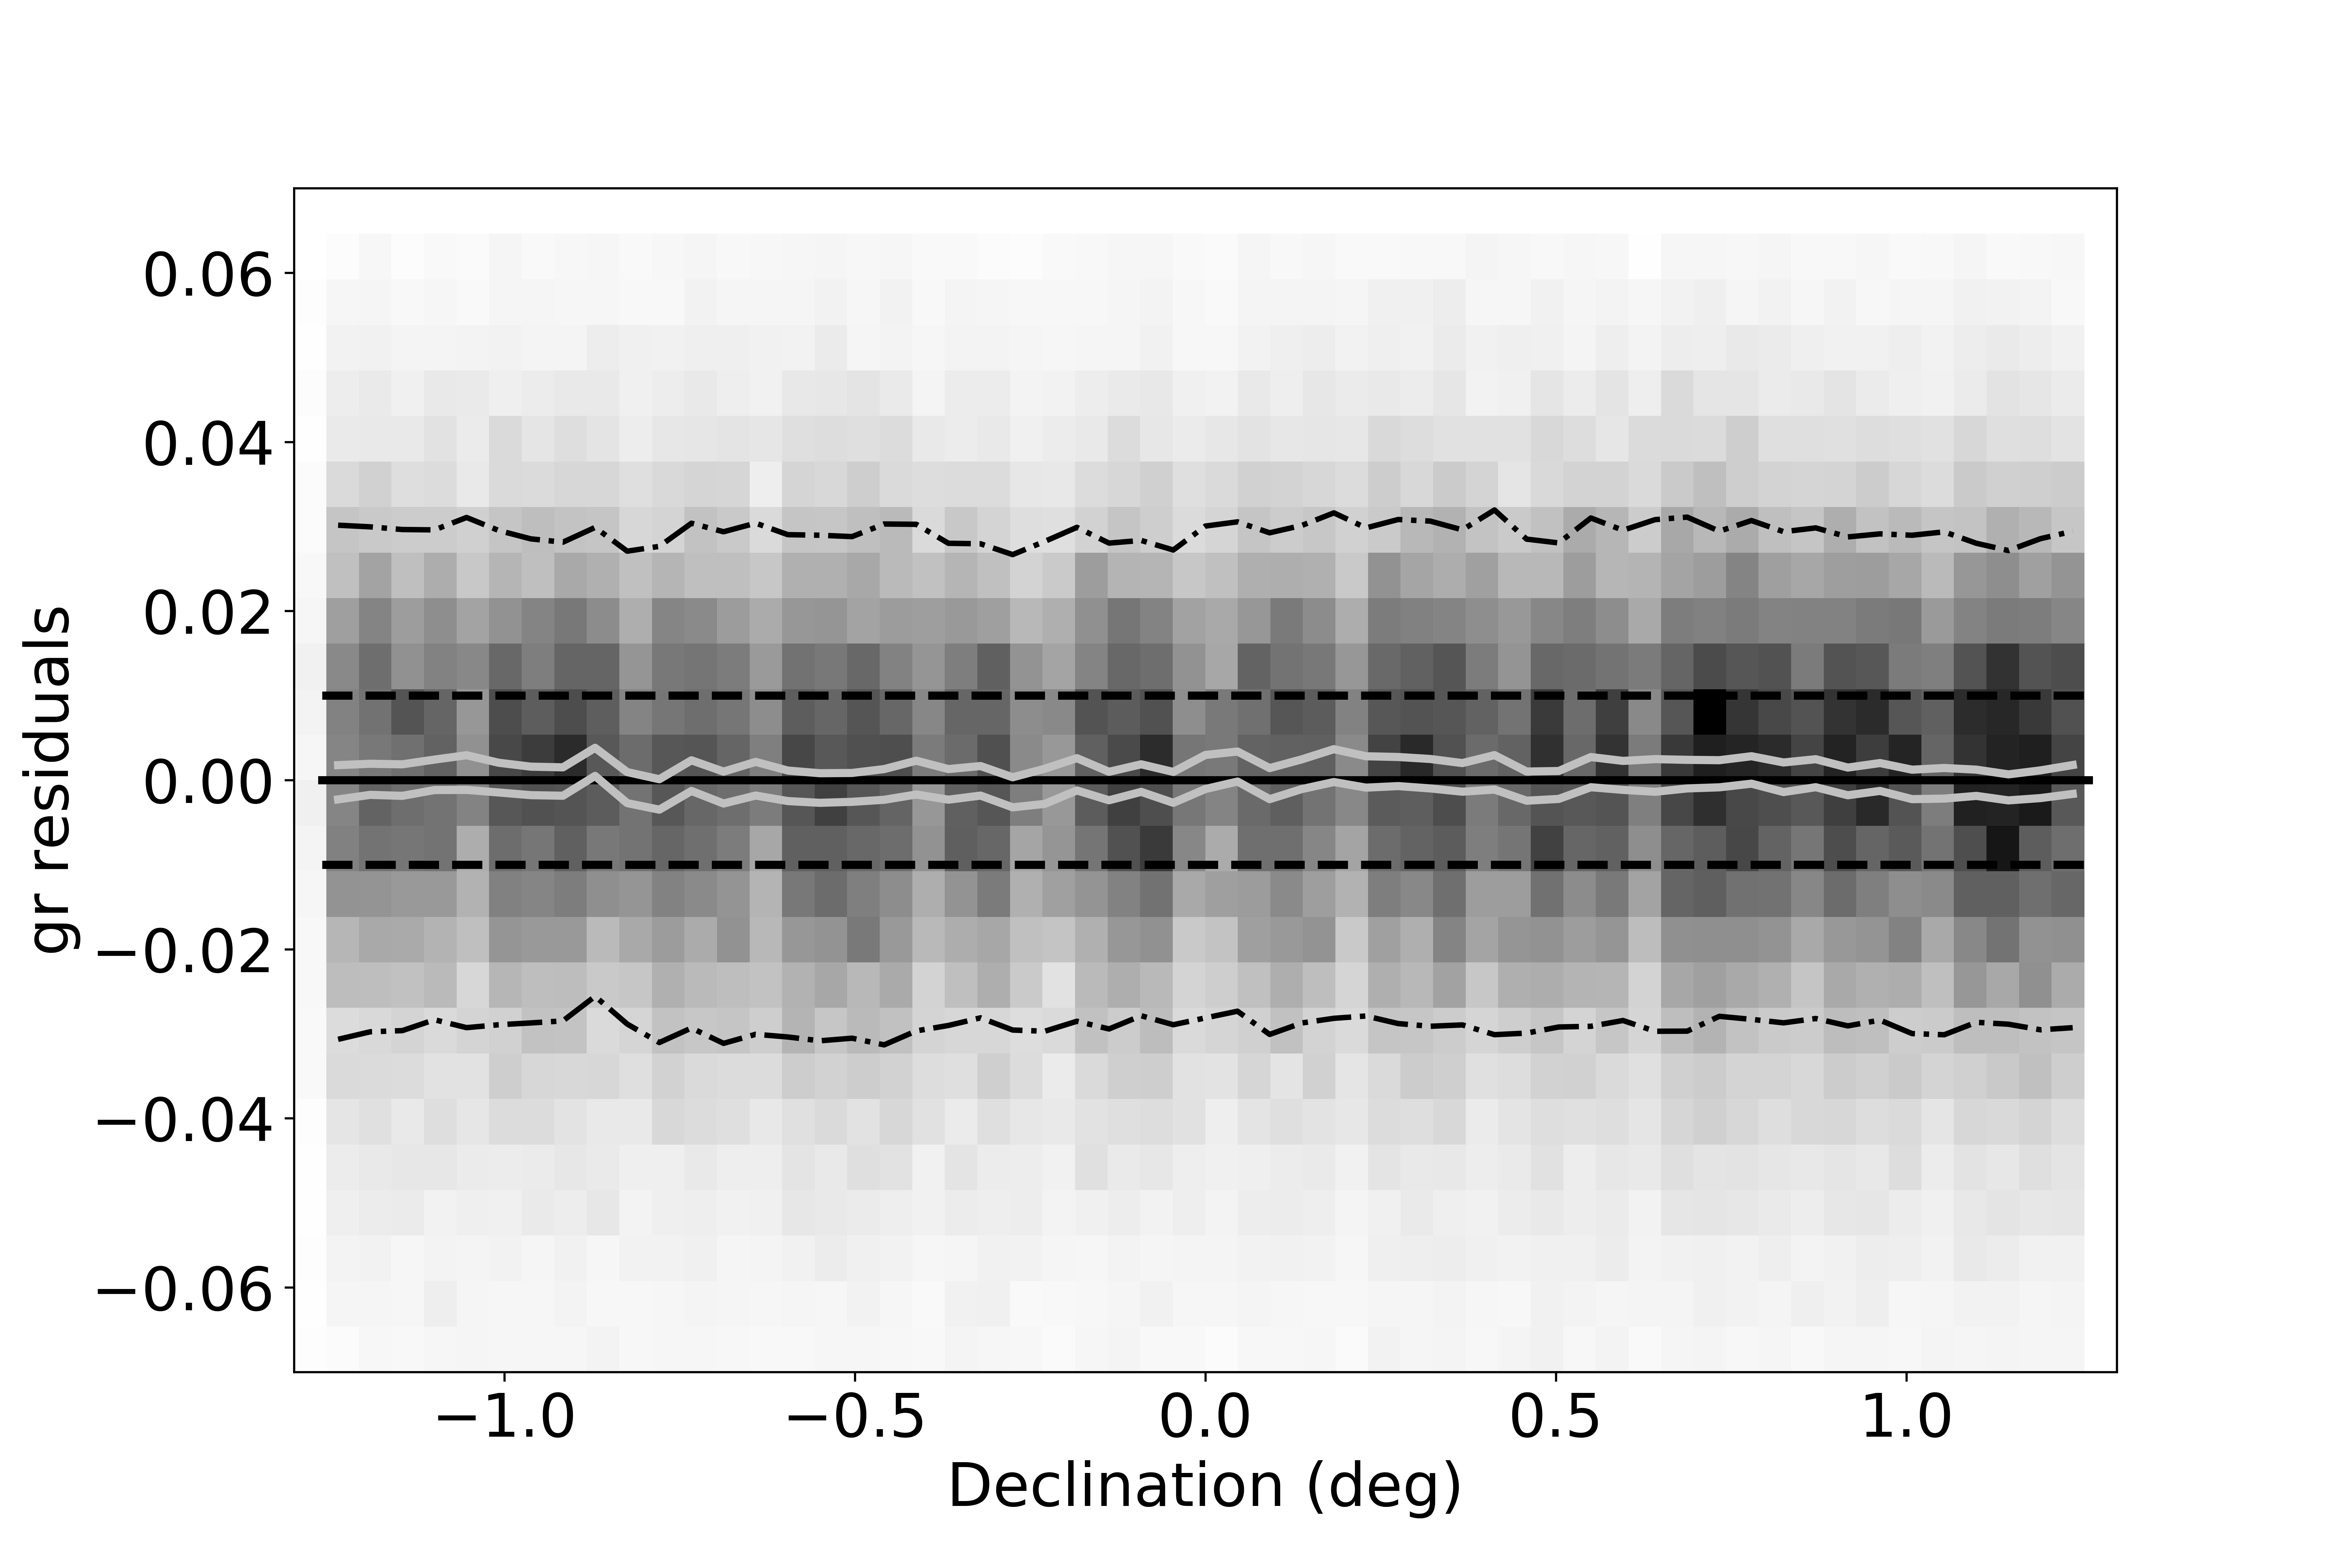
\includegraphics[width=7cm]{figures/colorResidGaiaColors_gr_Dec_Hess.png} 
\caption{Left: analogous to Figure~\ref{fig:graycorrRA}, except that here residuals between
the SDSS $g-r$ color from the v3.4 catalog and a synthetic $g-r$ color generated using 
Gaia's $BP-RP$ color are shown. The binned median scatter is 1.6 millimag. Right: the 
$g-r$ residuals are shown as a function of Declination. The binned median scatter is 
0.8 millimag.}
\label{fig:grVSgaiaRADec}
\end{figure}
 
 %%%%%%%%%%%%%%%%%%%%%%%%%%%%%%%%%%%%%%%%%

\subsection{Comparison of the SDSS v2.6 and v3.4 catalogs \label{sec:v26v34}} 
 
The v2.6 (``old'') SDSS Standard Star Catalog has been extensively used 
\citep[e.g.,][]{2008AJ....135..338F},
and here we briefly analyze differences between the v3.4 (``new'') and v2.6 magnitudes
to inform the future users about catalog consistency. 
In our analysis, we first compare v2.6 and v3.4 magnitudes of individual stars and 
bin the differences by R.A., Declination and magnitude. 

On average, both catalog versions are on the same magnitude scale (the median $ugriz$ 
magnitude differences for all stars are zero by construction). There are no systematic offsets 
when binned by magnitude, as illustrated in Figure~\ref{fig:v26v34drr}. The most obvious 
differences appear when magnitude differences are binned by Declination. An example is 
shown in Figure~\ref{fig:v26v34drDec}, where the periodicity of residuals corresponds to the 
field-of-view size for the SDSS Photometric Calibration Telescope \citep{2002AJ....123.2121S}. 
The standard deviation for median values per bin is 6.8 millimag, with extreme values about 
0.01 mag. It is likely that systematic errors in the calibration star network photometry 
were propagated through ``flat-field corrections'' discussed by \pO\ to the v2.6 catalog.
We note that these errors, now found thanks to Gaia catalogs, are well within the claimed
photemetric accuracy by both \pO\ and \cite{2002AJ....123.2121S}. The standard deviation 
for median values per bin for all bands and both coordinates is listed in Table~\ref{tab:oldnewRMS}. 


\begin{deluxetable}{l|c|c}[ht!]
\tablecaption{The robust standard deviation for magnitude differences between the v2.6 (old)
and v3.4 (new) catalogs. \label{tab:oldnewRMS}}
\tablehead{
\colhead{Band} & \colhead{rms for R.A.} & \colhead{rms for Dec}
}
\startdata
       $u$        &        2.3$^a$    &    25.5      \\
       $g$        &        4.5    &      9.4      \\  
       $r$         &        2.0    &      7.0      \\  
       $i$         &        5.3    &      6.5      \\ 
       $z$        &        8.9    &      8.4      \\ 
\enddata
\tablenotetext{a}{For the $u$ band, the scatter in R.A. direction is due to more observations
in v3.4 than in v2.6, rather than zeropoint correction.} 
\end{deluxetable}
   


\begin{figure}[th!]
    \centering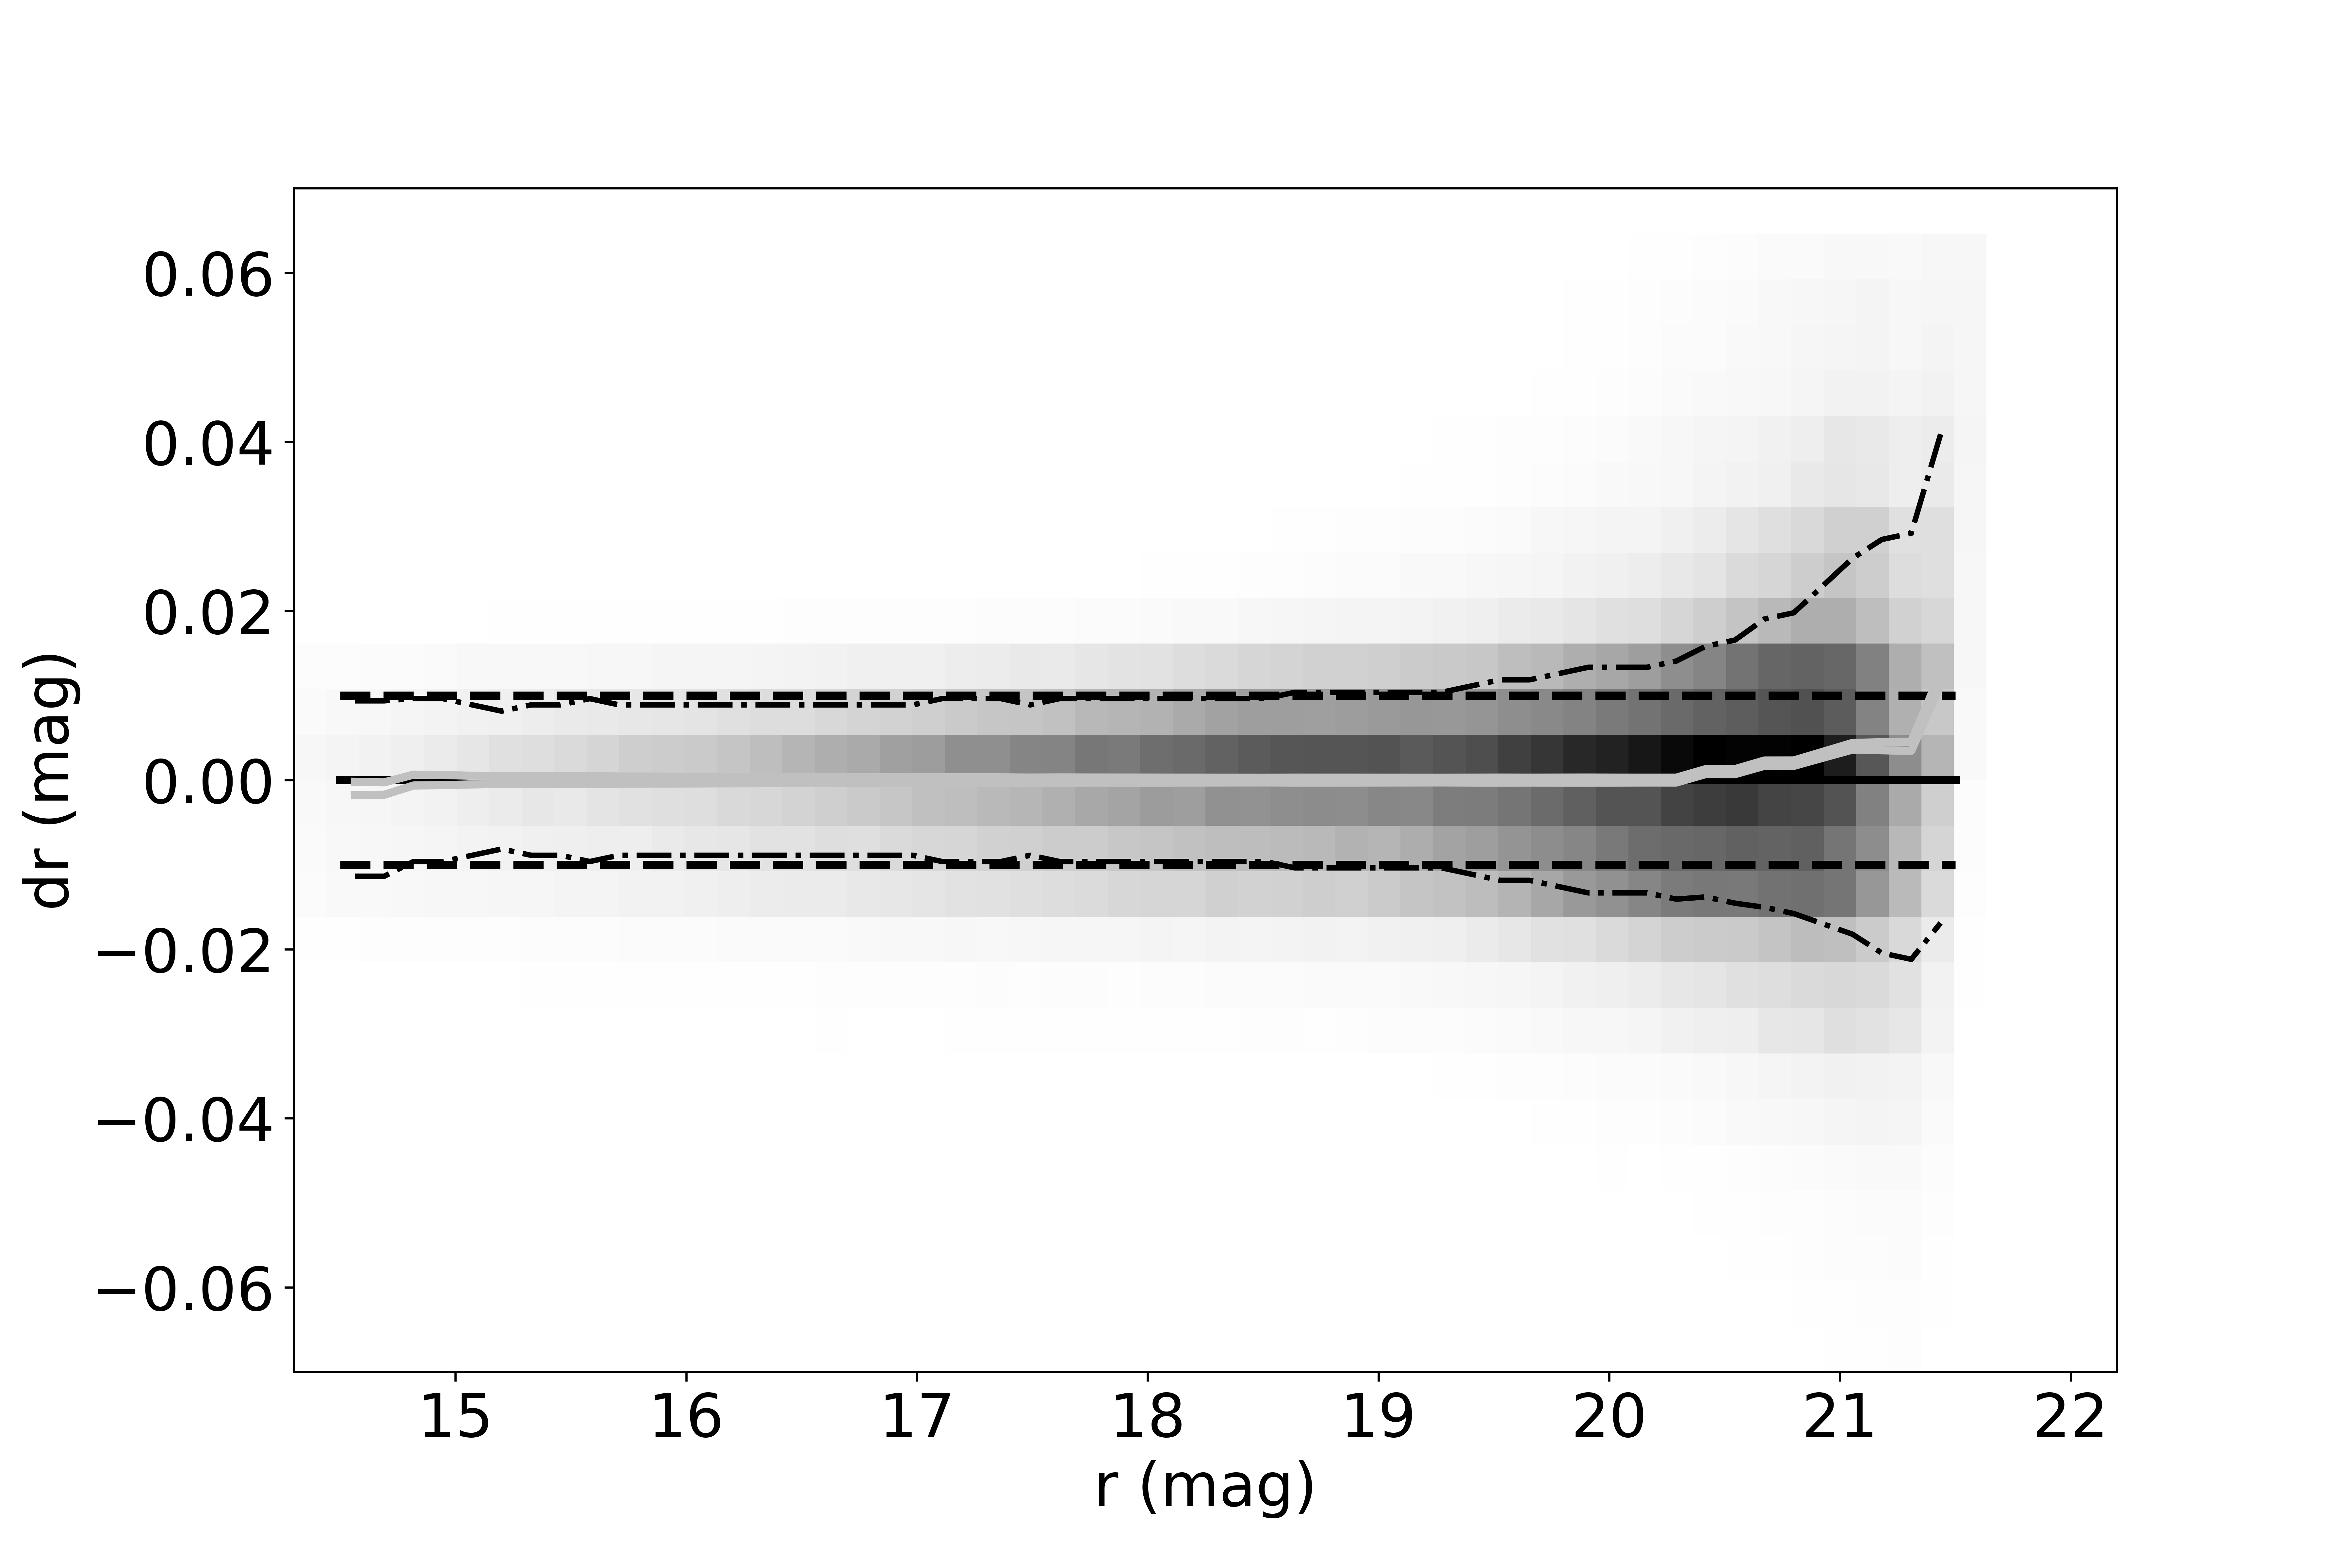
\includegraphics[width=9cm]{figures/testV26vsV33_r_dr_r_mag_Hess.png} 
\caption{Analogous to Figure~\ref{fig:v26v34drDec}, except that here the $r$ band
differences are shown as a function of the $r$ band magnitude. The scatted of median
values per bin is 1.9 millimag. The scatter of individual values is $\sim0.01$ mag
for $r<20$, and it is due to more data in the new catalog.} 
\label{fig:v26v34drr}
\end{figure}


\begin{figure}[th!]
    \centering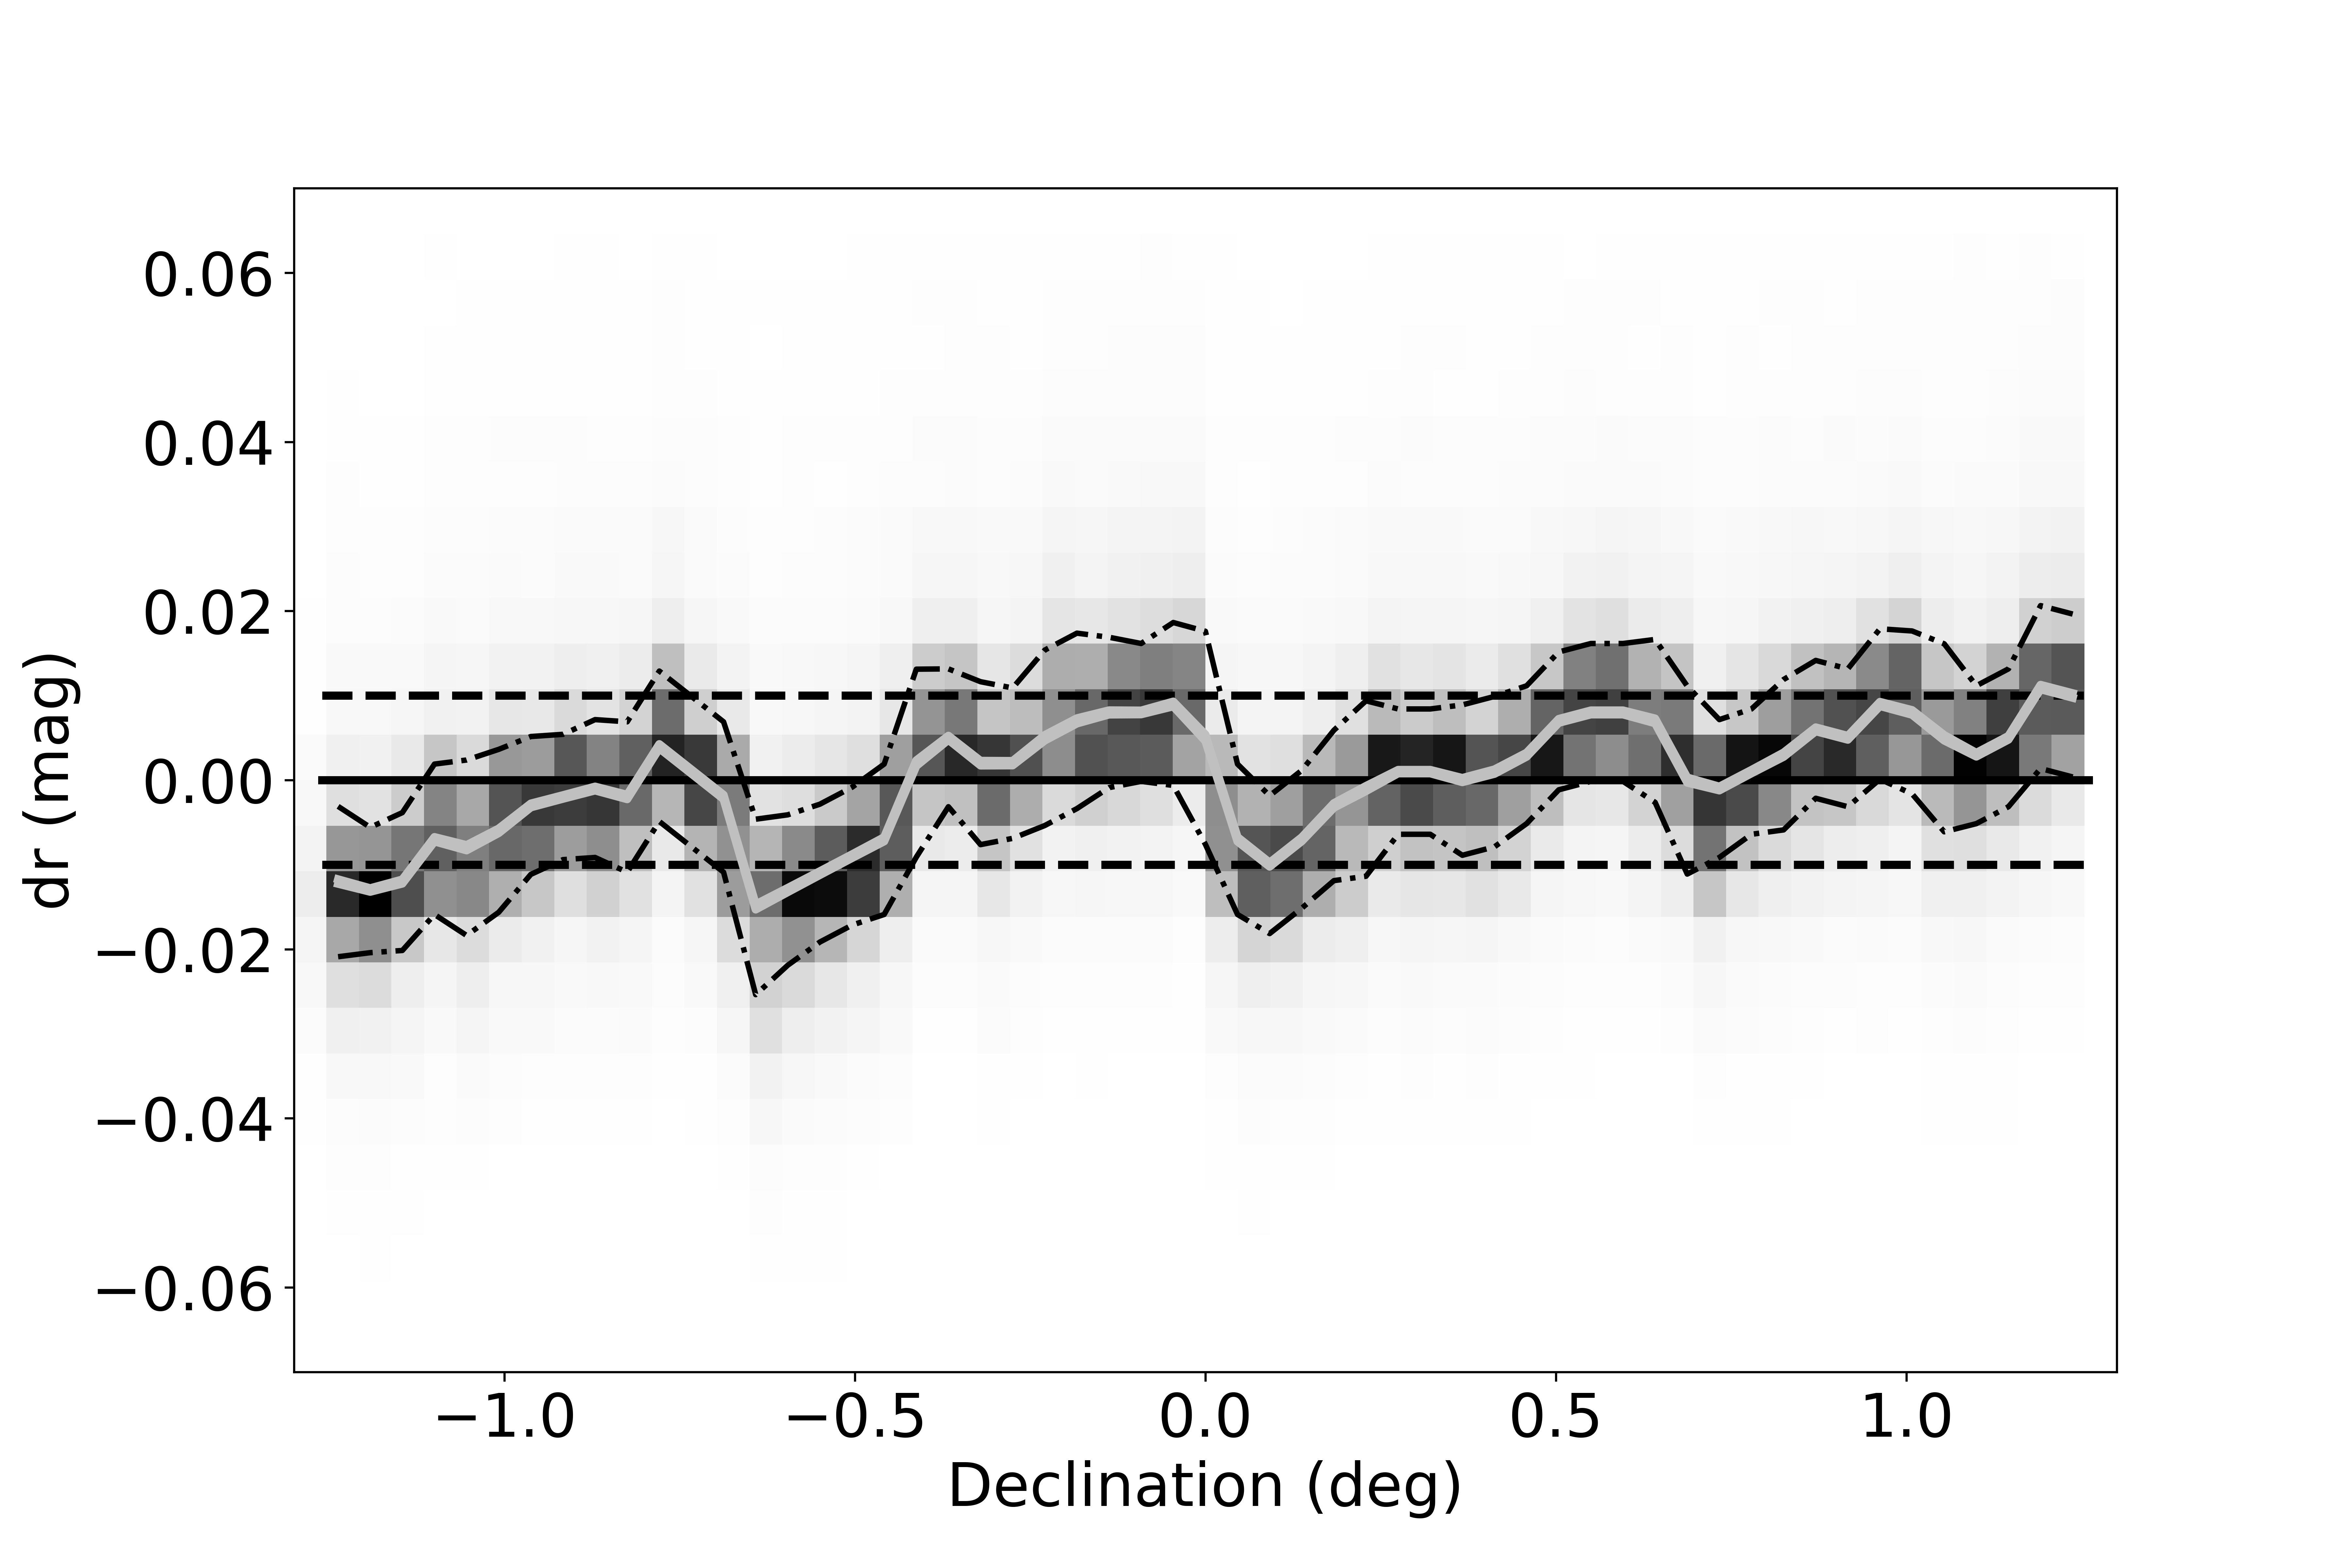
\includegraphics[width=9cm]{figures/testV26vsV33_r_dr_Dec_Hess.png} 
\caption{The differences between $r$ band magnitudes listed in the v2.6 and v3.4 
    SDSS Standard Star catalogs. The size of the four regions corresponds to the
field-of-view size of the SDSS Photometric Calibration Telescope. The standard 
deviation for median values per bin is 6.8 millimag, with extreme values about 0.01 mag. 
The scatter of binned medians in R.A. direction is much smaller -- 2.0 millimag. 
For statistics in other bands, please see Table~\ref{tab:oldnewRMS}.}
\label{fig:v26v34drDec}
\end{figure}
 


Given the quality of Gaia photometry, there should be no doubt that SDSS $ugriz$ photometry
reported in the new v.3.4 catalog is superior to the old v2.6 catalog. Nevertheless, we perform
additional tests, based on the position of the stellar locus in the $g-r$ vs. $u-g$, $r-i$ vs. $g-r$ 
and $i-z$ vs. $r-i$ color-color diagrams  \citep{2004AN....325..583I}. The tests are based
on the second principal color for the blue part of the stellar locus, whose median should 
not deviate from zero by construction. Figure~\ref{fig:comparew} compares the behavior
of the $w$ color for the old v2.6 and new v3.4 catalog and demonstrates that the $gri$
photometry is better calibrated in the latter. The behavior of the $s$ and $y$ colors for the 
new catalog is shown in Figure~\ref{fig:comparesy}. {\it Based on these tests, we find that 
the contribution of the zeropoint errors is $<5$ millimag to $gri$ photometry, and 
$<10$ millimag for the $u$ and $z$ bands.} 



\begin{figure}[th!]
    \centering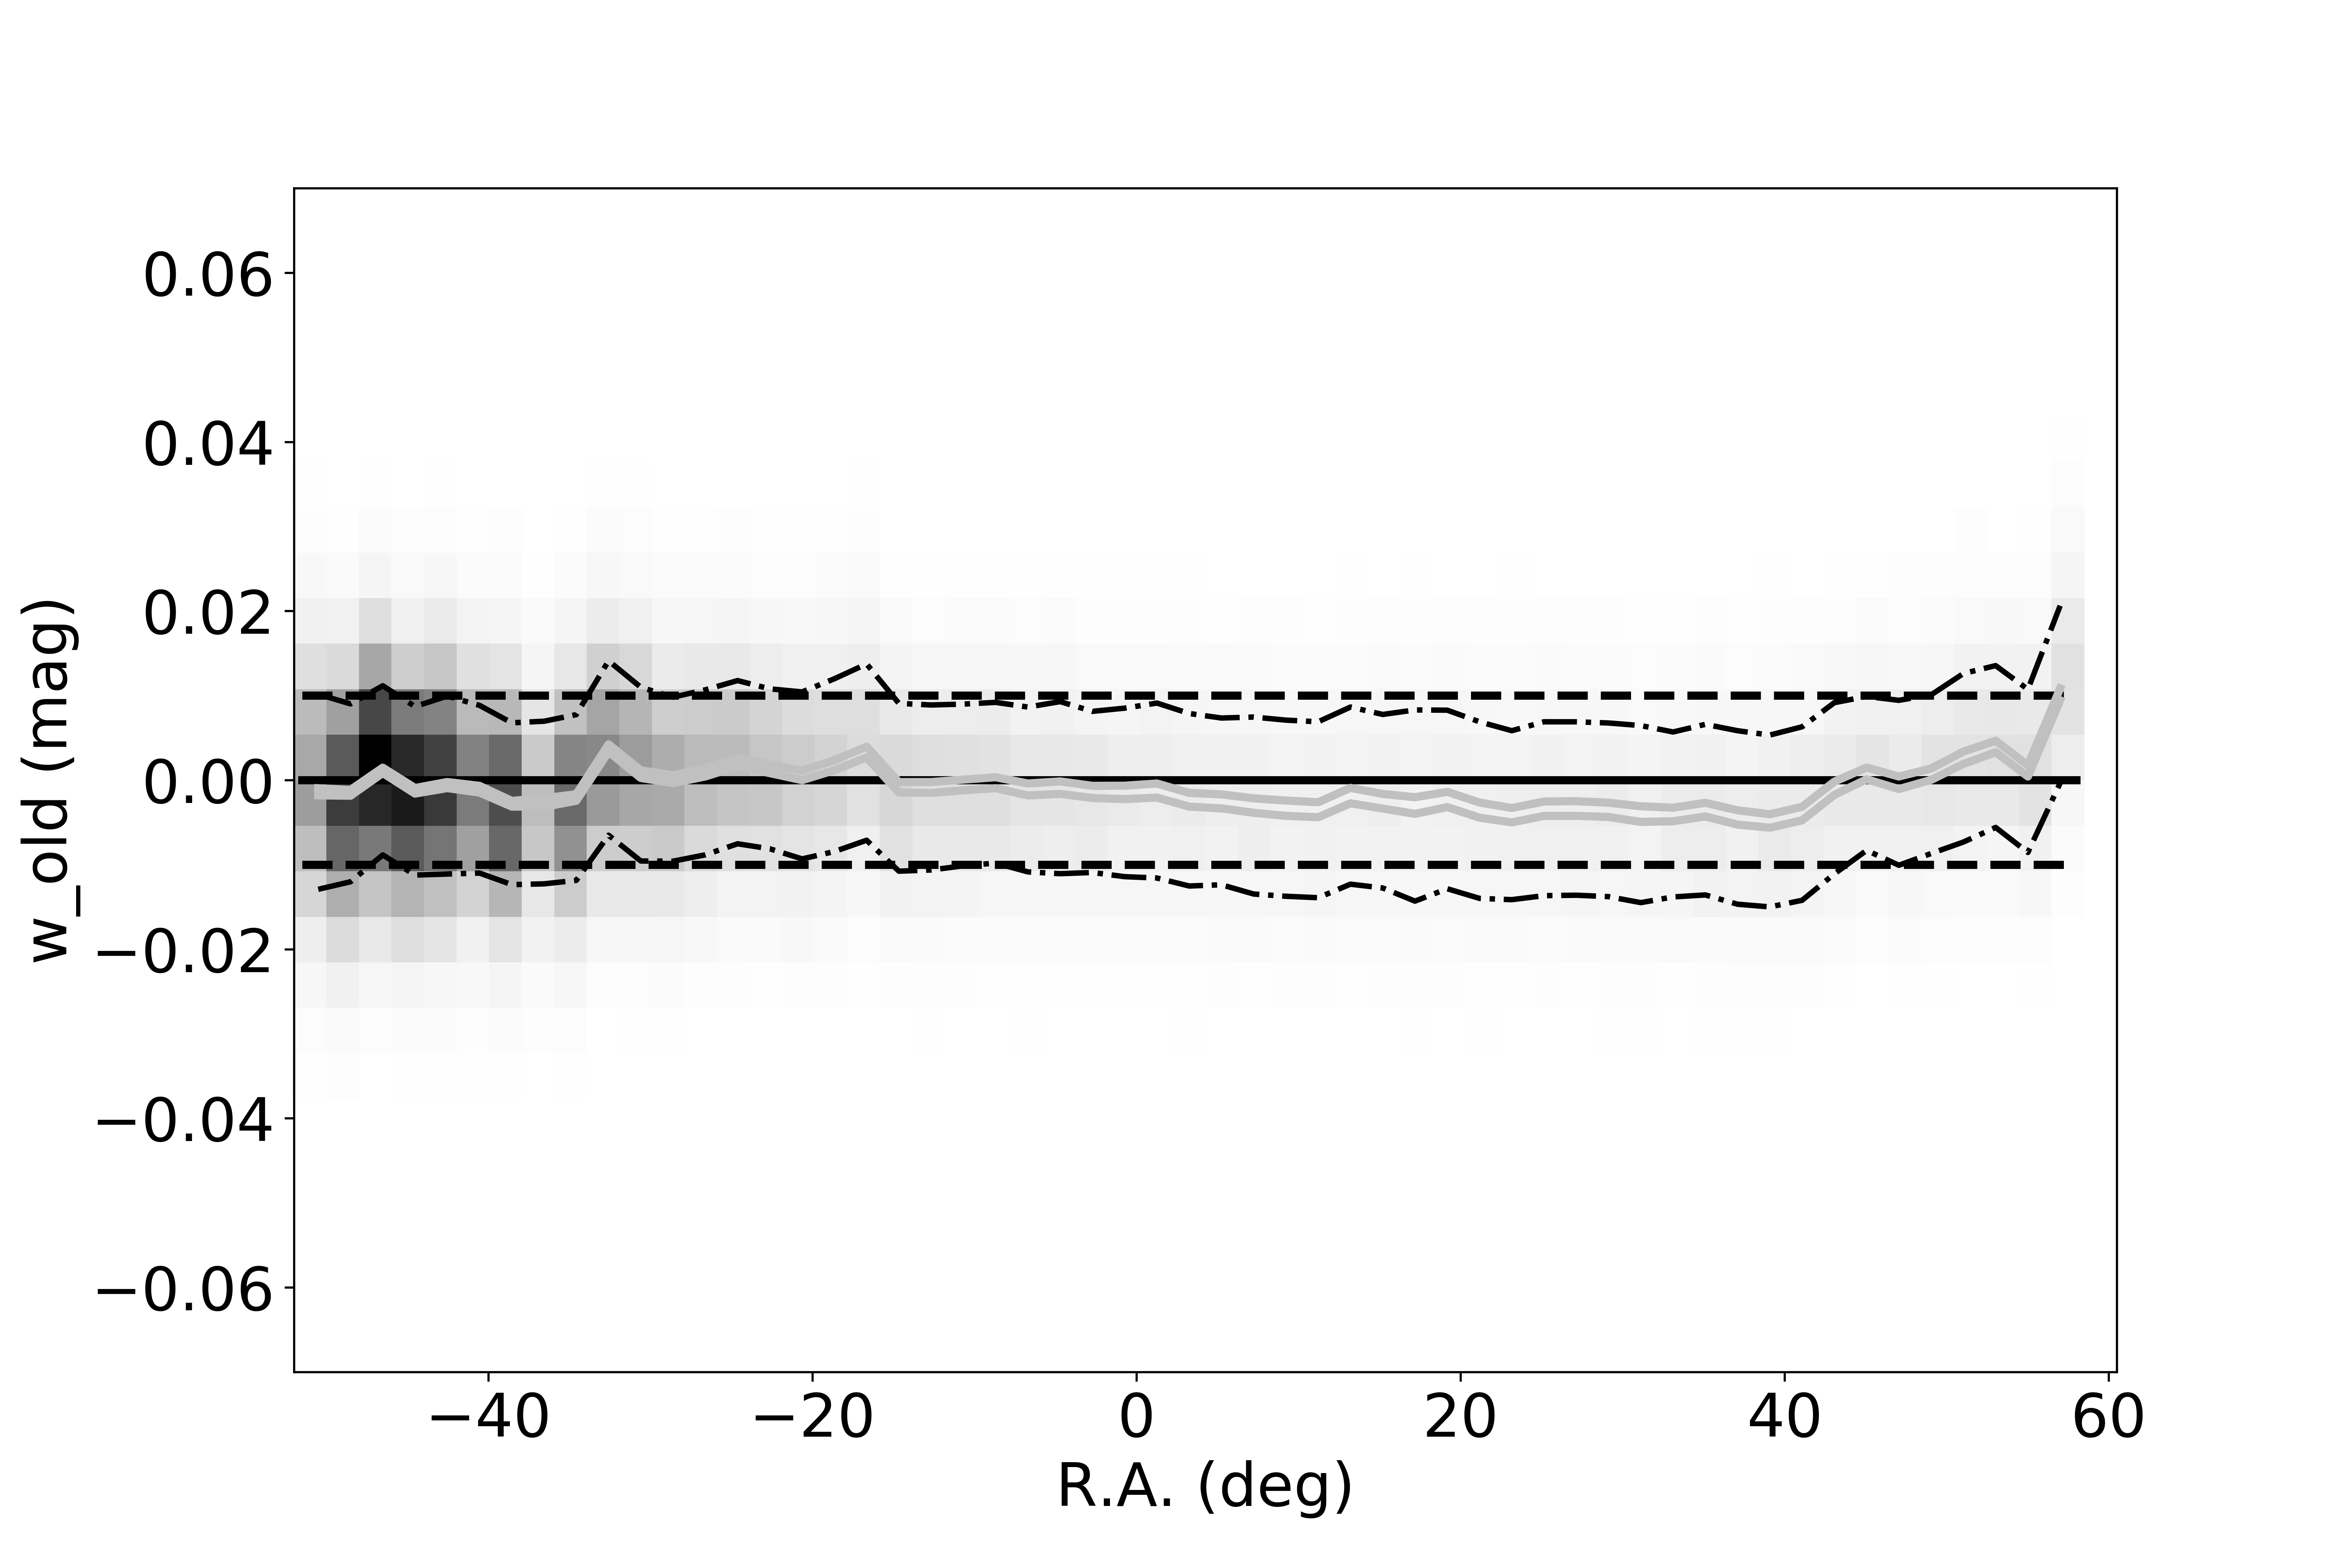
\includegraphics[width=7cm]{figures/testV26vsV33_r_w_old_RA_Hess.png}
    \centering\includegraphics[width=7cm]{figures/testV26vsV33_r_w_new_RA_Hess.png}
    \centering\includegraphics[width=7cm]{figures/testV26vsV33_r_w_old_Dec_Hess.png}
    \centering\includegraphics[width=7cm]{figures/testV26vsV33_r_w_new_Dec_Hess.png}
\caption{A comparison of the $w$ color, the second principal color in the SDSS
$r-i$ vs. $g-r$ color-color diagram, behavior for the v2.6 (left) and v3.4 (right)
catalogs. The standard deviation of the median $w$ values binned by R.A. and Dec
is 2.6 millimag and 1.1 millimag for v2.6 and 1.0 millimag and 0.3 millimag for v3.4,
respectively.}
\label{fig:comparew} 
\end{figure}
 

\begin{figure}[th!]
    \centering\includegraphics[width=7cm]{figures/testV26vsV33_snew_u_s_new_RA_Hess.png}
    \centering\includegraphics[width=7cm]{figures/testV26vsV33_snew_u_s_new_Dec_Hess.png} 
    \centering\includegraphics[width=7cm]{figures/testV26vsV33_ynew_z_y_new_RA_Hess.png} 
    \centering\includegraphics[width=7cm]{figures/testV26vsV33_ynew_z_y_new_Dec_Hess.png}  
\caption{The behavior of the $s$ color (top two panels), the second principal color in the SDSS
$g-r$ vs. $u-g$ color-color diagram, and the $y$ color (bottom two panels), the second 
principal color in the SDSS $i-z$ vs. $r-i$ color-color diagram, for the new v3.4 catalog.
The standard deviation of the median $s$ values binned by R.A. and Declination is 9.8 millimag 
and 1.3 millimag, respectively, and 1.8 millimag and 3.4 millimag for the $y$ color.}
\label{fig:comparesy} 
\end{figure}
  
%%%%%%%%%%%%%%%%%%%%%%%%%%%%%%%%%%%%%%%%%

\subsection{Comparison of the new v3.4 SDSS catalog with DES and Pan-STARRS catalogs \label{sec:DESPS1}} 
  
The quality of photometric zeropoint calibration for the new SDSS catalog can be conveniently
tested with the DES (see Section~\ref{ssec:des}) and Pan-STARRS (see Section~\ref{ssec:ps1}) catalogs. 
Both catalogs list $griz$ photometry of sufficient precision for esentially all stars
from Stripe 82. Their photometric calibration procedures are expected to result in different 
spatial patterns and thus a cross-comparison with the v3.4 catalog can reveal residual problems
with zeropoint calibration. They are also deeper than Gaia DR2 catalog and thus can provide
further clues about the Gmag discrepancy at Gaia's faint end illustrated in Figure~\ref{fig:gaiaJump}. 

Our comparison of the magnitude differences is illustrated in Figures~\ref{fig:DESPSRA} and \ref{fig:DESPSDec},
and the robust standard deviation for binned median magnitude differences is listed in Table~\ref{tab:DESPS1}. 
This multi-survey comparison indicates that the spatial variation of photometric zero points in the 
updated SDSS catalog is well below 0.01 mag (rms), with typical values of 3-7 millimag in the R.A. 
direction and 1-2 millimag in the Declination direction. As discernible in the two bottom panels
in Figure~\ref{fig:DESPSRA}, there are systematic residual errors in the $z$ band zeropoint as a 
function of  Declination at the level of a few millimag. Note also implied DES $z$ band zeropoint errors 
of up to 0.01-0.02 mag, as a function of R.A. (see the bottom left panel in Figure~\ref{fig:DESPSRA}). 

The variation of the magnitude differences
with magnitude (see Figure~\ref{fig:drVSr}) shows good agreement (to within $\sim$5 millimag) 
even at the faint end ($20<r<21$), where Gaia Gmag magnitudes appear too faint by about
0.02 mag, and thus demonstrates a likely problem with Gaia DR2 photometry. 
 
\begin{deluxetable}{l|c|c|c|c}[ht!]
\tablecaption{The robust standard deviation for binned median magnitude differences between
the new v3.4 SDSS catalog, and DES and Pan-STARRS1 (PS1) catalogs (millimag). \label{tab:DESPS1}}
\tablehead{
\colhead{Band} & \colhead{DES R.A.} & \colhead{DES Dec} & \colhead{PS1 R.A.} & \colhead{PS1 Dec} 
}
\startdata
       $g$        &        5.1    &      1.8   &        3.4    &      1.4        \\
       $r$         &        4.1    &      0.8   &        2.6    &      0.7         \\  
       $i$         &        7.3    &      1.6   &        3.2    &      1.0         \\ 
       $z$        &       13.6    &     3.6   &        6.8    &      2.3         \\ 
\enddata
\end{deluxetable}
   

\begin{figure}[th!]
    \centering\includegraphics[width=7cm]{figures/colorResidDES2bright_dr_RA_Hess.png}
    \centering\includegraphics[width=7cm]{figures/colorResidPSbright_dr_RA_Hess.png}
    \centering\includegraphics[width=7cm]{figures/colorResidDES2bright_di_RA_Hess.png}
    \centering\includegraphics[width=7cm]{figures/colorResidPSbright_di_RA_Hess.png}
    \centering\includegraphics[width=7cm]{figures/colorResidDES2bright_dz_RA_Hess.png}
    \centering\includegraphics[width=7cm]{figures/colorResidPSbright_dz_RA_Hess.png}
\caption{A comparison of the magnitude differences between the SDSS v3.4 catalog
and DES (left) and Pan-STARRS (right) catalogs, for the $riz$ bands.}
\label{fig:DESPSRA}
\end{figure}

\begin{figure}[th!]
    \centering\includegraphics[width=7cm]{figures/colorResidDES2bright_dr_Dec_Hess.png}
    \centering\includegraphics[width=7cm]{figures/colorResidPSbright_dr_Dec_Hess.png}
    \centering\includegraphics[width=7cm]{figures/colorResidDES2bright_di_Dec_Hess.png}
    \centering\includegraphics[width=7cm]{figures/colorResidPSbright_di_Dec_Hess.png}
    \centering\includegraphics[width=7cm]{figures/colorResidDES2bright_dz_Dec_Hess.png}
    \centering\includegraphics[width=7cm]{figures/colorResidPSbright_dz_Dec_Hess.png}
\caption{Analogous to Figure~\ref{fig:DESPSRA}, except that magnitude differences
are binned by Declination.}
\label{fig:DESPSDec}
\end{figure}

\begin{figure}[th!]
    \centering\includegraphics[width=7cm]{figures/colorResidDES2_dr_rmag_Hess.png}
    \centering\includegraphics[width=7cm]{figures/colorResidDES2_di_rmag_Hess.png} 
\caption{A comparison of the magnitude differences between the SDSS v3.4 catalog
and DES catalog, for the $r$ and $i$ bands. Note the good agreement even at the
faint end ($20<r<21$), where Gaia Gmag magnitudes appear too faint by about
0.02 mag (see Figure~\ref{fig:gaiaJump}).} 
\label{fig:drVSr}
\end{figure}

%%%%%%%%%%%%%%%%%%%%%%%%%%%%%%%%%%%%%%%%%


\subsection{Comparison of the new v3.4 SDSS catalog and $u$ band data from the CFIS catalog  \label{sec:CFIStest}} 

The comparison of the new SDSS catalog with the DES and Pan-STARRS catalogs in the previous
section did not include the $u$ band. To assess the quality of $u$ band zeropoint calibration, 
we use the CFIS catalog (see Section~\ref{ssec:cfis}). The CFIS $u$ band photometry was 
calibrated using a combination of the SDSS, Pan-STARRS and GALEX UV data. Given that
we recalibrated the new SDSS catalog using Gaia data, for this comparison it shouldn't 
matter that SDSS data were used in calibration of the CFIS catalog. Nevertheless, the
results of this section should be treated with caution. 

A star-by-star comparison for about 150,000 sufficiently bright ($r<20$) blue ($1.0 <u-g < 2.1$) 
stars is illustrated in Figure~\ref{fig:CFIS}. The binned median scatter for Declination direction is 
5.7 millimag with systematic differences of up to about 0.01 mag. The constraints in R.A. direction 
are more noisy, with residuals appearing about twice as large as in Declination direction. 
These residuals compare favorably to the results of analysis by \cite{2017ApJ...848..128I}, 
who showed that some SDSS runs in Data Release 13 have $u$-band zeropoint errors as large
as 0.05 mag. 

 
\begin{figure}[th!]
    \centering\includegraphics[width=9cm]{figures/colorResidCFISug_Dec_Hess.png} 
\caption{Analogous to Figure~\ref{fig:graycorrDec}, except that here residuals 
between the SDSS $u$ band magnitudes and $u$ band magnitudes from the CFIS
catalog (corrected for small color terms, $\sim0.05$ mag, as a function of the $u-g$ color),
for $\sim$150,000 matched stars with $1.0 <u-g < 2.1$ and $r<20$ are shown. 
The binned median scatter is 5.7 millimag. Note that the CFIS data are available
only for Declination $>$ -0.45 degree.}
\label{fig:CFIS}
\end{figure}

%%%%%%%%%%%%%%%%%%%%%%%%%%%%%%%%%%%%%%%%%
\subsection{Comparison of the new v3.4 SDSS catalog and transformed nUV data from the GALEX catalog  \label{sec:Galextest}} 

We also use the NUV magnitudes from GALEX (see Section~\ref{ssec:galex}) to provide an independent check on the SDSS u-band magnitudes, following the zeropoint corrections with Gaia photometry described in \S \ref{sec:GaiaCorr}. For this we derive 
GALEX to SDSS u transformation equations. Using GALEX NUV with SDSS (g,i) or with SDSS (r,i) yields the tightest GALEX to SDSS u transformation equation:
 
 \begin{equation}
 % \begin{multline}
 \begin{split}
  u_sdss = & NUV_{galex} + 0.939 \\
                  & - 1.008*(NUV_{galex} -- g_{sdss}) + 0.017*(NUV_{galex} -- g_{sdss})^2 \\
                  & -- 0.599*(g_{sdss} -- i_{sdss}) + 0.860*(g_{sdss} -- i_{sdss})^2
 \end{split}
%  \end{multline}
\end{equation}
 
Quality plots for this fit are shown in Figure \ref{fig:GalexQA} {\bf need to redo these plots in BW; select subplots to include}. The rms per star for this relation is 0.071 mag ? so still a bit noisy, but about as good as we think we can get for transforming GALEX to SDSS u (but see below regarding E(B-V)?).
 
 \begin{figure}[th!]
    \centering\includegraphics[width=14cm]{figures/Galex_QA.png}
\caption{{\bf  To be filled}} 
\label{fig:GalexQA}
\end{figure}
    
The quality plots for this fit can be found in the attached plot,
%%   sdss_galex_transform_u.20180614.norder2.niter3.uNUV.NUVg.gi_sdss.qa1.png
 
In the next plot,
%%  stripe82calibStars_v3.4_vs_GALEX_u-band_plot1.png ,
is plotted the 2D sky distribution of the matches, binned into 0.21-sq-deg healpixels, with each bin color coded to show the median difference between the SDSS $u_{mMed}$ mag and the GALEX-transformed $u_{mMed-est}$ in the healpixel.
 
The next plot,
%%  stripe82calibStars_v3.4_vs_GALEX_u-band_plot2.png ,
is the same as the previous plot, but now the healpixels are color coded by the median SFD98 E(B-V) in that healpixel.
Note that there is a slight correlation between these two plots.
 
In the final plot,
%%  stripe82calibStars_v3.4_vs_GALEX_u-band_plot3.png ,
the difference between the observed $u_{mMed}$ magtitude and the GALEX-transformed $u_{mMed-est}$ for each star is plotted against SFD98 E(B-V).    So it looks like the above GALEX à SDSS u-band transformation starts to break down for E(B-V) $>$ 0.15.  Maybe the next step would be including E(B-V) explicitly into the fit for the transformation equation.  Either that, or try a first attempt at the 2D figures using Zeljko?s jupyter notebooks.

%%%%%%%%%%%%%%%%%%%%%%%%%%%%%%%%%%%%%%%%%

\subsection{Offsets from AB magnitude scale \label{sec:AB}} 

We estimate offsets from AB magnitude scale using photometry for three DA white dwarfs observed by HST
(see Table~\ref{tab:HST}). XXX Doug expands this section, refers to G. Narayan et al. (2019) and other refs,
and other details explaining how synthetic ugriz photometry is generated for these three stars...

% From Doug's email: 
% As to the precision and accuracy of the synthetic mags, that is a little hard to quantify.  Narayan et al (2019) report 
% uncertainties for the synthetic magnitudes of the 2 DA’s from their sample at about 0.5% (5 milli-mags), but I don’t know if 
% that includes uncertainties in the reddening and in version of the SDSS filters used.  The HST CalSpec database (which 
% included GD50) is usually quoted as having an accuracy of about 1% (10 milli-mags) in the optical on average for any given 
% star in its database. 
% When I get observed DA WD spectra modeled by Pier-Emmanuel Tremblay (a former postdoc of Bergeron), he sends me not 
% only the best-fit model but also the +/-1sigma Teff, logg models as well.  When I calculate the synthetic mags for those, I
% usually get a spread of less than 1% in the resulting synthetic mags; so I think Gautham Narayan’s estimate of a statistical
% rms of 0.5% for his models is reasonable.  So maybe 0.5% (5 millimag) precision/statistical error, and c. 1% (10 milli-mags)
% accuracy/systematic error.

Table~\ref{tab:AB} presents numerical summary of the comparison between SDSS magnitudes 
and HST-based synthetic magnitudes for three white dwarfs. We used unweighted mean because 
formal uncertainties for SDSS photometry are subdominant to systematic errors in HST-based
synthetic magnitudes, estimated at about 0.01 mag. Uncertainty of the mean offsets was 
computed from the observed scatter of three values. In the $riz$ bands we detect significant
($>3\sigma$) deviations, ranging from 0.015 mag to 0.035 mag, while in the $u$ and $g$ bands 
we can only place upper limits (at $2\sigma$: 0.038 mag and 0.028 mag, respectively). 

\begin{deluxetable}{r|r|l|l|l|l|l}[ht!]
\tablecaption{Synthetic SDSS magnitudes for three WD dwarfs with HST photometry$^a$. \label{tab:HST}}
\tablehead{
  \colhead{R.A. } & \colhead{Dec.} & \colhead{u} & \colhead{g} & \colhead{r} & \colhead{i} & \colhead{z} 
}
\startdata
    352.4221875 &        0.185500 &      18.154 &       18.145 &    18.466 &     18.754 &     19.042 \\  
      15.8424625 &  $-$0.346592 &      18.627 &       19.057 &    19.558 &     19.923 &     20.258 \\
      57.2091083 &  $-$0.975636 &      13.409 &       13.784 &    14.295 &     14.655 &     99.999$^b$ \\
\enddata
\tablenotetext{a}{Give here reference to HST data, or some other comment?} 
\tablenotetext{b}{The CalSpec spectrum stopped at about 9000 \AA and thus did not cover all of SDSS $z$ band.} 
\end{deluxetable}


\begin{deluxetable}{l|r|r|r|r|r}[ht!]
\tablecaption{AB offsets implied by three WD dwarfs with HST photometry$^a$. \label{tab:AB}}
\tablehead{
      & \colhead{$\Delta u$}  & \colhead{$\Delta g$}  & \colhead{$\Delta r$}  & \colhead{$\Delta i$}  & \colhead{$\Delta z$}  
}
\startdata 
   {\rm mean}            &    $-$0.009    &        0.000     &      0.015    &       0.016    &      0.035     \\ 
  $\sigma_{\rm mean}$ &         0.019    &        0.014     &      0.004    &       0.004    &      0.011     \\
\enddata
\tablenotetext{a}{Offsets are defined as additive corrections to SDSS photometry to place it on AB scale (in mag). 
Listed values are unweighted mean and its uncertainty.}  
\end{deluxetable}
  % This contains a sec on Galex

%%%%%%%%%%%%%%%%%%%%%%%%%%%%%%%%%%%%%%%%%%%%%%%%%%
\section{Discussion and Conclusions} \label{sec:disc}

To enable further progress in cosmological and other high-precision photometric measurements, 
modern multi-band photometric sky surveys aim to deliver measurements accurate at the 1\% 
(0.01 mag) level. Over the last decade a number of such large-scale surveys approached, and
often exceeded this photometric accuracy threshold. For ground-based surveys, that are 
affected by variable atmospheric effects and hardware responses to changes in local environment
(e.g. temperature), significant improvements can be achieved by averaging multiple observations. 

In this paper, we have described the construction and tests of an updated version of the so-called
SDSS Stripe 82 Standard Star catalog \citep{Ivez07} that lists averaged SDSS photometry for about
a million non-variable stars. Additional post-2007 SDSS data include about 
2-3 times more measurements per star than in the original catalog, resulting in 1.4-1.7 times smaller 
random photometric errors (precision) than in the original catalog, and about three times as small 
as for individual SDSS runs.

Thanks to the availability of photometric data from recent wide-field surveys (Gaia, DES, Pan-STARRS
and CFIS), we were able to derive robust zeropoint corrections and establish that this new catalog
is superior to the original catalog. Using a combination of comparison to other catalogs and 
astrophysical constraints, we find that that the contribution of the zeropoint errors to photometric
uncertainties is $<5$ millimag for the $gri$ bands, and $<10$ millimag for the $u$ and $z$ bands. 

Various catalog cross-comparisons have revealed minor problems with all the analyzed catalogs.
For example, we detected DES $z$ band zeropoint errors of up to 0.01-0.02 mag, as a function 
of R.A., and demonstrated that Gaia Gmag magnitudes appear too faint by about 0.02 mag at
Gmag$\sim$20.
 
We constrained offsets from the absolute AB magnitude scale using three white dwarfs with the 
HST CalSpec absolute photometry data. In the $riz$ bands we measured significant ($>3\sigma$) 
deviations, ranging from 0.015 mag to 0.035 mag (see Table~\ref{tab:AB}), while in the $u$ and $g$ 
bands we only placed upper limits (at $2\sigma$: 0.038 mag and 0.028 mag, respectively). These
constraints on absolute AB magnitude scale could be improved by extend the number of such 
calibrators.

Thanks to its high stellar density, about 1 star per square arcmin, and demonstrated sub-percent 
internal photometric precision, this catalog is a good resource for both calibrating and testing 
other surveys. In particular, it will enable high-precision photometric testing of data collected 
during the commissioning phase of the Rubin Observatory Legacy Survey of Space and Time. 
  
%%%%%%%%%%%%%%%%%%%%%%%%%%%%%%%%%%%%%%%%%%%%%%%%%%%

\acknowledgments

We thank Stephen Gwyn for providing the CFIS catalog to us, and for discussions of the
$u$ band photometry. 

Funding for the SDSS and SDSS-II has been provided by the Alfred P. Sloan Foundation, the Participating
Institutions, the National Science Foundation, the US Department of Energy, the National Aeronautics and 
Space Administration, the Japanese Monbukagakusho, the Max Planck Society, and the Higher Education 
Funding Council for England. The SDSS Web site is http://www.sdss.org.
 
\vspace{5mm}
\facilities{SDSS, Pan-STARRS, DECam, CFHT}

\software{numpy \citep{numpy}, matplotlib \citep{Hunter:2007}, scipy \citep{scipy}, 
       astropy \citep{astropy-1, astropy-2}, astroML \citep{2012cidu.conf...47V}.}

%%%%%%%%%%%%%%%%%%%%%
%% BIBLIOGRAPHY
\bibliography{S82SSC}{}
\bibliographystyle{aasjournal}

%\appendix
%\section{Appendix information}
%
%Here is Appendix A.
 
\end{document}
